% Options for packages loaded elsewhere
% Options for packages loaded elsewhere
\PassOptionsToPackage{unicode}{hyperref}
\PassOptionsToPackage{hyphens}{url}
\PassOptionsToPackage{dvipsnames,svgnames,x11names}{xcolor}
%
\documentclass[
  letterpaper,
  DIV=11,
  numbers=noendperiod]{scrreprt}
\usepackage{xcolor}
\usepackage{amsmath,amssymb}
\setcounter{secnumdepth}{5}
\usepackage{iftex}
\ifPDFTeX
  \usepackage[T1]{fontenc}
  \usepackage[utf8]{inputenc}
  \usepackage{textcomp} % provide euro and other symbols
\else % if luatex or xetex
  \usepackage{unicode-math} % this also loads fontspec
  \defaultfontfeatures{Scale=MatchLowercase}
  \defaultfontfeatures[\rmfamily]{Ligatures=TeX,Scale=1}
\fi
\usepackage{lmodern}
\ifPDFTeX\else
  % xetex/luatex font selection
\fi
% Use upquote if available, for straight quotes in verbatim environments
\IfFileExists{upquote.sty}{\usepackage{upquote}}{}
\IfFileExists{microtype.sty}{% use microtype if available
  \usepackage[]{microtype}
  \UseMicrotypeSet[protrusion]{basicmath} % disable protrusion for tt fonts
}{}
\makeatletter
\@ifundefined{KOMAClassName}{% if non-KOMA class
  \IfFileExists{parskip.sty}{%
    \usepackage{parskip}
  }{% else
    \setlength{\parindent}{0pt}
    \setlength{\parskip}{6pt plus 2pt minus 1pt}}
}{% if KOMA class
  \KOMAoptions{parskip=half}}
\makeatother
% Make \paragraph and \subparagraph free-standing
\makeatletter
\ifx\paragraph\undefined\else
  \let\oldparagraph\paragraph
  \renewcommand{\paragraph}{
    \@ifstar
      \xxxParagraphStar
      \xxxParagraphNoStar
  }
  \newcommand{\xxxParagraphStar}[1]{\oldparagraph*{#1}\mbox{}}
  \newcommand{\xxxParagraphNoStar}[1]{\oldparagraph{#1}\mbox{}}
\fi
\ifx\subparagraph\undefined\else
  \let\oldsubparagraph\subparagraph
  \renewcommand{\subparagraph}{
    \@ifstar
      \xxxSubParagraphStar
      \xxxSubParagraphNoStar
  }
  \newcommand{\xxxSubParagraphStar}[1]{\oldsubparagraph*{#1}\mbox{}}
  \newcommand{\xxxSubParagraphNoStar}[1]{\oldsubparagraph{#1}\mbox{}}
\fi
\makeatother

\usepackage{color}
\usepackage{fancyvrb}
\newcommand{\VerbBar}{|}
\newcommand{\VERB}{\Verb[commandchars=\\\{\}]}
\DefineVerbatimEnvironment{Highlighting}{Verbatim}{commandchars=\\\{\}}
% Add ',fontsize=\small' for more characters per line
\usepackage{framed}
\definecolor{shadecolor}{RGB}{241,243,245}
\newenvironment{Shaded}{\begin{snugshade}}{\end{snugshade}}
\newcommand{\AlertTok}[1]{\textcolor[rgb]{0.68,0.00,0.00}{#1}}
\newcommand{\AnnotationTok}[1]{\textcolor[rgb]{0.37,0.37,0.37}{#1}}
\newcommand{\AttributeTok}[1]{\textcolor[rgb]{0.40,0.45,0.13}{#1}}
\newcommand{\BaseNTok}[1]{\textcolor[rgb]{0.68,0.00,0.00}{#1}}
\newcommand{\BuiltInTok}[1]{\textcolor[rgb]{0.00,0.23,0.31}{#1}}
\newcommand{\CharTok}[1]{\textcolor[rgb]{0.13,0.47,0.30}{#1}}
\newcommand{\CommentTok}[1]{\textcolor[rgb]{0.37,0.37,0.37}{#1}}
\newcommand{\CommentVarTok}[1]{\textcolor[rgb]{0.37,0.37,0.37}{\textit{#1}}}
\newcommand{\ConstantTok}[1]{\textcolor[rgb]{0.56,0.35,0.01}{#1}}
\newcommand{\ControlFlowTok}[1]{\textcolor[rgb]{0.00,0.23,0.31}{\textbf{#1}}}
\newcommand{\DataTypeTok}[1]{\textcolor[rgb]{0.68,0.00,0.00}{#1}}
\newcommand{\DecValTok}[1]{\textcolor[rgb]{0.68,0.00,0.00}{#1}}
\newcommand{\DocumentationTok}[1]{\textcolor[rgb]{0.37,0.37,0.37}{\textit{#1}}}
\newcommand{\ErrorTok}[1]{\textcolor[rgb]{0.68,0.00,0.00}{#1}}
\newcommand{\ExtensionTok}[1]{\textcolor[rgb]{0.00,0.23,0.31}{#1}}
\newcommand{\FloatTok}[1]{\textcolor[rgb]{0.68,0.00,0.00}{#1}}
\newcommand{\FunctionTok}[1]{\textcolor[rgb]{0.28,0.35,0.67}{#1}}
\newcommand{\ImportTok}[1]{\textcolor[rgb]{0.00,0.46,0.62}{#1}}
\newcommand{\InformationTok}[1]{\textcolor[rgb]{0.37,0.37,0.37}{#1}}
\newcommand{\KeywordTok}[1]{\textcolor[rgb]{0.00,0.23,0.31}{\textbf{#1}}}
\newcommand{\NormalTok}[1]{\textcolor[rgb]{0.00,0.23,0.31}{#1}}
\newcommand{\OperatorTok}[1]{\textcolor[rgb]{0.37,0.37,0.37}{#1}}
\newcommand{\OtherTok}[1]{\textcolor[rgb]{0.00,0.23,0.31}{#1}}
\newcommand{\PreprocessorTok}[1]{\textcolor[rgb]{0.68,0.00,0.00}{#1}}
\newcommand{\RegionMarkerTok}[1]{\textcolor[rgb]{0.00,0.23,0.31}{#1}}
\newcommand{\SpecialCharTok}[1]{\textcolor[rgb]{0.37,0.37,0.37}{#1}}
\newcommand{\SpecialStringTok}[1]{\textcolor[rgb]{0.13,0.47,0.30}{#1}}
\newcommand{\StringTok}[1]{\textcolor[rgb]{0.13,0.47,0.30}{#1}}
\newcommand{\VariableTok}[1]{\textcolor[rgb]{0.07,0.07,0.07}{#1}}
\newcommand{\VerbatimStringTok}[1]{\textcolor[rgb]{0.13,0.47,0.30}{#1}}
\newcommand{\WarningTok}[1]{\textcolor[rgb]{0.37,0.37,0.37}{\textit{#1}}}

\usepackage{longtable,booktabs,array}
\usepackage{calc} % for calculating minipage widths
% Correct order of tables after \paragraph or \subparagraph
\usepackage{etoolbox}
\makeatletter
\patchcmd\longtable{\par}{\if@noskipsec\mbox{}\fi\par}{}{}
\makeatother
% Allow footnotes in longtable head/foot
\IfFileExists{footnotehyper.sty}{\usepackage{footnotehyper}}{\usepackage{footnote}}
\makesavenoteenv{longtable}
\usepackage{graphicx}
\makeatletter
\newsavebox\pandoc@box
\newcommand*\pandocbounded[1]{% scales image to fit in text height/width
  \sbox\pandoc@box{#1}%
  \Gscale@div\@tempa{\textheight}{\dimexpr\ht\pandoc@box+\dp\pandoc@box\relax}%
  \Gscale@div\@tempb{\linewidth}{\wd\pandoc@box}%
  \ifdim\@tempb\p@<\@tempa\p@\let\@tempa\@tempb\fi% select the smaller of both
  \ifdim\@tempa\p@<\p@\scalebox{\@tempa}{\usebox\pandoc@box}%
  \else\usebox{\pandoc@box}%
  \fi%
}
% Set default figure placement to htbp
\def\fps@figure{htbp}
\makeatother





\setlength{\emergencystretch}{3em} % prevent overfull lines

\providecommand{\tightlist}{%
  \setlength{\itemsep}{0pt}\setlength{\parskip}{0pt}}



 


\KOMAoption{captions}{tableheading}
\makeatletter
\@ifpackageloaded{tcolorbox}{}{\usepackage[skins,breakable]{tcolorbox}}
\@ifpackageloaded{fontawesome5}{}{\usepackage{fontawesome5}}
\definecolor{quarto-callout-color}{HTML}{909090}
\definecolor{quarto-callout-note-color}{HTML}{0758E5}
\definecolor{quarto-callout-important-color}{HTML}{CC1914}
\definecolor{quarto-callout-warning-color}{HTML}{EB9113}
\definecolor{quarto-callout-tip-color}{HTML}{00A047}
\definecolor{quarto-callout-caution-color}{HTML}{FC5300}
\definecolor{quarto-callout-color-frame}{HTML}{acacac}
\definecolor{quarto-callout-note-color-frame}{HTML}{4582ec}
\definecolor{quarto-callout-important-color-frame}{HTML}{d9534f}
\definecolor{quarto-callout-warning-color-frame}{HTML}{f0ad4e}
\definecolor{quarto-callout-tip-color-frame}{HTML}{02b875}
\definecolor{quarto-callout-caution-color-frame}{HTML}{fd7e14}
\makeatother
\makeatletter
\@ifpackageloaded{bookmark}{}{\usepackage{bookmark}}
\makeatother
\makeatletter
\@ifpackageloaded{caption}{}{\usepackage{caption}}
\AtBeginDocument{%
\ifdefined\contentsname
  \renewcommand*\contentsname{Table of contents}
\else
  \newcommand\contentsname{Table of contents}
\fi
\ifdefined\listfigurename
  \renewcommand*\listfigurename{List of Figures}
\else
  \newcommand\listfigurename{List of Figures}
\fi
\ifdefined\listtablename
  \renewcommand*\listtablename{List of Tables}
\else
  \newcommand\listtablename{List of Tables}
\fi
\ifdefined\figurename
  \renewcommand*\figurename{Figure}
\else
  \newcommand\figurename{Figure}
\fi
\ifdefined\tablename
  \renewcommand*\tablename{Table}
\else
  \newcommand\tablename{Table}
\fi
}
\@ifpackageloaded{float}{}{\usepackage{float}}
\floatstyle{ruled}
\@ifundefined{c@chapter}{\newfloat{codelisting}{h}{lop}}{\newfloat{codelisting}{h}{lop}[chapter]}
\floatname{codelisting}{Listing}
\newcommand*\listoflistings{\listof{codelisting}{List of Listings}}
\makeatother
\makeatletter
\makeatother
\makeatletter
\@ifpackageloaded{caption}{}{\usepackage{caption}}
\@ifpackageloaded{subcaption}{}{\usepackage{subcaption}}
\makeatother
\usepackage{bookmark}
\IfFileExists{xurl.sty}{\usepackage{xurl}}{} % add URL line breaks if available
\urlstyle{same}
\hypersetup{
  pdftitle={Introduction to Data Science with R},
  pdfauthor={Jon McCurdy},
  colorlinks=true,
  linkcolor={blue},
  filecolor={Maroon},
  citecolor={Blue},
  urlcolor={Blue},
  pdfcreator={LaTeX via pandoc}}


\title{Introduction to Data Science with R}
\author{Jon McCurdy}
\date{2025-05-03}
\begin{document}
\maketitle

\renewcommand*\contentsname{Table of contents}
{
\hypersetup{linkcolor=}
\setcounter{tocdepth}{2}
\tableofcontents
}

\bookmarksetup{startatroot}

\chapter*{Preface}\label{preface}
\addcontentsline{toc}{chapter}{Preface}

\markboth{Preface}{Preface}

\begin{itemize}
\tightlist
\item
  Understand the basics of regression analysis.
\item
  Learn how to interpret p-values and confidence intervals.
\item
  Apply regression in R to a real dataset.
\end{itemize}

This is a Quarto book.

To learn more about Quarto books visit
\url{https://quarto.org/docs/books}.

\begin{Shaded}
\begin{Highlighting}[]
\DecValTok{1} \SpecialCharTok{+} \DecValTok{1}
\end{Highlighting}
\end{Shaded}

\begin{verbatim}
[1] 2
\end{verbatim}

\begin{Shaded}
\begin{Highlighting}[]
\DecValTok{3}\SpecialCharTok{+}\DecValTok{2}
\end{Highlighting}
\end{Shaded}

\begin{verbatim}
[1] 5
\end{verbatim}

\begin{Shaded}
\begin{Highlighting}[]
\NormalTok{linear\_model }\OtherTok{\textless{}{-}} \FunctionTok{lm}\NormalTok{(Sepal.Length }\SpecialCharTok{\textasciitilde{}}\NormalTok{ Sepal.Width, }\AttributeTok{data=}\NormalTok{iris)}
\FunctionTok{summary}\NormalTok{(linear\_model)}
\end{Highlighting}
\end{Shaded}

\begin{verbatim}

Call:
lm(formula = Sepal.Length ~ Sepal.Width, data = iris)

Residuals:
    Min      1Q  Median      3Q     Max 
-1.5561 -0.6333 -0.1120  0.5579  2.2226 

Coefficients:
            Estimate Std. Error t value Pr(>|t|)    
(Intercept)   6.5262     0.4789   13.63   <2e-16 ***
Sepal.Width  -0.2234     0.1551   -1.44    0.152    
---
Signif. codes:  0 '***' 0.001 '**' 0.01 '*' 0.05 '.' 0.1 ' ' 1

Residual standard error: 0.8251 on 148 degrees of freedom
Multiple R-squared:  0.01382,   Adjusted R-squared:  0.007159 
F-statistic: 2.074 on 1 and 148 DF,  p-value: 0.1519
\end{verbatim}

\section*{Watch this video}\label{watch-this-video}
\addcontentsline{toc}{section}{Watch this video}

\markright{Watch this video}

We can add a video fairly easily with the following code (modestbranding
reduces logo and rel=0 does not suggest other channels when paused)

(https://quarto.org/docs/authoring/videos.html)

\url{https://www.youtube.com/embed/iAF7APi_EgU?modestbranding=1&rel=0}

\section*{Callout Boxes}\label{callout-boxes}
\addcontentsline{toc}{section}{Callout Boxes}

\markright{Callout Boxes}

We can make callout boxes for note, warning, important, tip, and caution

(https://quarto.org/docs/authoring/callouts.html)

\begin{tcolorbox}[enhanced jigsaw, opacitybacktitle=0.6, bottomtitle=1mm, left=2mm, opacityback=0, colframe=quarto-callout-note-color-frame, toptitle=1mm, rightrule=.15mm, colback=white, titlerule=0mm, coltitle=black, toprule=.15mm, leftrule=.75mm, title=\textcolor{quarto-callout-note-color}{\faInfo}\hspace{0.5em}{Note}, arc=.35mm, bottomrule=.15mm, colbacktitle=quarto-callout-note-color!10!white, breakable]

Note that there are five types of callouts, including: \texttt{note},
\texttt{warning}, \texttt{important}, \texttt{tip}, and
\texttt{caution}.

\end{tcolorbox}

\begin{tcolorbox}[enhanced jigsaw, opacitybacktitle=0.6, bottomtitle=1mm, left=2mm, opacityback=0, colframe=quarto-callout-tip-color-frame, toptitle=1mm, rightrule=.15mm, colback=white, titlerule=0mm, coltitle=black, toprule=.15mm, leftrule=.75mm, title=\textcolor{quarto-callout-tip-color}{\faLightbulb}\hspace{0.5em}{Tip with Title}, arc=.35mm, bottomrule=.15mm, colbacktitle=quarto-callout-tip-color!10!white, breakable]

This is an example of a callout with a title.

\end{tcolorbox}

\begin{tcolorbox}[enhanced jigsaw, opacitybacktitle=0.6, bottomtitle=1mm, left=2mm, opacityback=0, colframe=quarto-callout-caution-color-frame, toptitle=1mm, rightrule=.15mm, colback=white, titlerule=0mm, coltitle=black, toprule=.15mm, leftrule=.75mm, title=\textcolor{quarto-callout-caution-color}{\faFire}\hspace{0.5em}{Expand To Learn About Collapse}, arc=.35mm, bottomrule=.15mm, colbacktitle=quarto-callout-caution-color!10!white, breakable]

This is an example of a `folded' caution callout that can be expanded by
the user. You can use \texttt{collapse="true"} to collapse it by default
or \texttt{collapse="false"} to make a collapsible callout that is
expanded by default.

\end{tcolorbox}

\begin{tcolorbox}[enhanced jigsaw, opacitybacktitle=0.6, bottomtitle=1mm, left=2mm, opacityback=0, colframe=quarto-callout-tip-color-frame, toptitle=1mm, rightrule=.15mm, colback=white, titlerule=0mm, coltitle=black, toprule=.15mm, leftrule=.75mm, title=\textcolor{quarto-callout-tip-color}{\faLightbulb}\hspace{0.5em}{Tip with Title}, arc=.35mm, bottomrule=.15mm, colbacktitle=quarto-callout-tip-color!10!white, breakable]

This is a callout with a title.

\end{tcolorbox}

\section*{Sample Questions for
Students}\label{sample-questions-for-students}
\addcontentsline{toc}{section}{Sample Questions for Students}

\markright{Sample Questions for Students}

\begin{tcolorbox}[enhanced jigsaw, opacitybacktitle=0.6, bottomtitle=1mm, left=2mm, opacityback=0, colframe=quarto-callout-tip-color-frame, toptitle=1mm, rightrule=.15mm, colback=white, titlerule=0mm, coltitle=black, toprule=.15mm, leftrule=.75mm, title=\textcolor{quarto-callout-tip-color}{\faLightbulb}\hspace{0.5em}{Try it Out}, arc=.35mm, bottomrule=.15mm, colbacktitle=quarto-callout-tip-color!10!white, breakable]

What is the output of \texttt{mean(c(1,\ 2,\ 3,\ 4,\ 5))} in R?

\begin{quote}
\textbf{Solution}

The output is \texttt{3}. This is because it calculates the arithmetic
mean:\\
(1 + 2 + 3 + 4 + 5) / 5 = 15 / 5 = 3.
\end{quote}

\end{tcolorbox}

\section*{Creating Problems for Students to
Try}\label{creating-problems-for-students-to-try}
\addcontentsline{toc}{section}{Creating Problems for Students to Try}

\markright{Creating Problems for Students to Try}

\begin{tcolorbox}[enhanced jigsaw, opacitybacktitle=0.6, bottomtitle=1mm, left=2mm, opacityback=0, colframe=quarto-callout-tip-color-frame, toptitle=1mm, rightrule=.15mm, colback=white, titlerule=0mm, coltitle=black, toprule=.15mm, leftrule=.75mm, title=\textcolor{quarto-callout-tip-color}{\faLightbulb}\hspace{0.5em}{Try it Out}, arc=.35mm, bottomrule=.15mm, colbacktitle=quarto-callout-tip-color!10!white, breakable]

What is the output of \texttt{mean(c(1,\ 2,\ 3,\ 4,\ 5))} in R?

Click to see the solution

The output is \texttt{3}. This is because it calculates the arithmetic
mean:\\
(1 + 2 + 3 + 4 + 5) / 5 = 15 / 5 = 3.

\end{tcolorbox}

\section*{Creating Quiz Questions for
Students}\label{creating-quiz-questions-for-students}
\addcontentsline{toc}{section}{Creating Quiz Questions for Students}

\markright{Creating Quiz Questions for Students}

(https://web.mat.upc.edu/joaquim.puig/posts/webexercises-quiz/)

\begin{itemize}
\item
  \textbf{Numeric questions} How much is 2+3? \_
\item
  \textbf{Multiple Choice} Which is the capital city of Barbados?
\item
  \begin{enumerate}
  \def\labelenumi{(\Alph{enumi})}
  \tightlist
  \item
    Bridgetown\\
  \end{enumerate}
\item
  \begin{enumerate}
  \def\labelenumi{(\Alph{enumi})}
  \setcounter{enumi}{1}
  \tightlist
  \item
    Georgetown\\
  \end{enumerate}
\item
  \begin{enumerate}
  \def\labelenumi{(\Alph{enumi})}
  \setcounter{enumi}{2}
  \tightlist
  \item
    Kingston\\
  \end{enumerate}
\item
  \begin{enumerate}
  \def\labelenumi{(\Alph{enumi})}
  \setcounter{enumi}{3}
  \tightlist
  \item
    Bridgerton
  \end{enumerate}
\item
  \textbf{True or False} Quarto is very cool TRUE / FALSE.
\item
  \textbf{Fill in the Blank} What is the letter after D? \_.
\item
  Type a vowel: \_
\item
  Which function will help me find standard deviation for the code:
  \_\_(c(1,4,7,8,4))
\end{itemize}

Testing 123

\bookmarksetup{startatroot}

\chapter{What is Data?}\label{what-is-data}

As we begin our journey to becoming Data Scientists, it is important to
get a firm grasp of what data actually is. There are many ways to define
data. If you were to look at the origin of the word, you would see that
it is the plural of the Latin word ``datum'', which means piece of
information. You might propose other definitions, such as; Information
collected about something, or Facts and Statistics used to calculate
something. All of these are acceptable interpretations of data, and we
will probably switch between them throughout the semester. But, it is
important to acknowledge that data (the individual pieces of
information) by itself is essentially meaningless, it is through
interpretation that it gains meaning. And that is what we will learn
throughout this semester; how to interpret pieces of information to tell
a story.

\begin{itemize}
\tightlist
\item
  Understand the basics of what data looks like.
\item
  Learn how to interpret p-values and confidence intervals.
\item
  Apply regression in R to a real dataset.
\end{itemize}

\section{Data-fication}\label{data-fication}

Technology has become an integral part of our daily life. Almost
everything we do tracks and collects data on us. This includes checking
our social media in the morning, purchasing food with our credit card,
and even ``scanning'' our ID to enter buildings. Every company we
interact with collects data on us whether we like it or not, including
the Government. It should be mentioned that not all of this is bad. The
school collects information about what classes you have passed, credit
card companies collect information to determine how reliable you are in
paying your bills, and hospitals collect medical history about you to
improve your level of care.

Before reading on, you should stop and think about what information
about you is out there. Can you think of specific companies/groups which
have a lot of data bout you? Do you think it is a good or bad thing that
information about you is collected?

Because of the large amount of data that is floating around in the
``wild'', scientists say that we are currently in the ``Age of
Information/Data''. Another term, coined in a 2013 article titled ``The
Rise of Big Data'', describes the process of ``taking all aspects of
life and turning them into data {[}\(\dots\){]} Once we datafy things,
we can transform their purpose and turn the information into new forms
of value.'' This results in a ``digital footprint''; as we leave a trail
of data about ourselves wherever we go. This digit footprint starts when
we are born and follows us throughout our lives. Companies are able to
change/tweak products based on the data they collect about our
preferences (think how social media evolved based on the apps we used),
but these products can also change how we behave (think social media
addiction).

\section{Communicating with Data}\label{communicating-with-data}

So all of this data is available, but why should we care exactly? Well,
all of this data allows us to do some pretty cool things. In the
previous section, we mentioned how credit card companies can determine
if we are dependable. They do this by taking our past payment history
and other information about us, such as age, gender, and income level,
and then building a model to decide if we will end up paying off the
loan or defaulting on it. Other scenarios might be to predict the
outcomes of NFL games, analyze weather patterns to better understand
hurricane trajectory, or even recommend movies on Netflix/products on
Amazon. All of these things are done with data, and when we build these
models we are doing Data Science. There are many definitions out there
for Data Science, but one of the ones I like is the following:
\textbf{Data Science unlocks hidden stories within vast amounts of data,
paving the way for innovations that transform industries and improve
lives.}

Since Data Science involves the process of unlocking and telling
stories, it is important for us to ask ourselves what exactly makes a
good story. In middle school and high school, I am sure we were taught
that every story should have a beginning (the Introduction), a middle
(the ``Plot''), and an ending (the Conclusion). As Data Scientists, we
will need to communicate our results in a similar way (as a data story)
in order for people to understand our findings. So, we should also start
to think about how we convey a data story so other people can understand
it. If we are predicting the miles per gallon a car will have, then we
will present our story differently to kindergartners than we would to
automotive experts. So, it is important to write our story with our
audience in mind. To help the presentation, we will want to incorporate
visualizations to engage the audience and support our plot.

\section{Classifying Data}\label{classifying-data}

There are a number of ways to classify the data that we will encounter
throughout this course. The first big division will be deciding whether
the data is \textbf{Quantitative} or \textbf{Qualitative}. Quantitative
data are anything that is a count or a measure (think quantities) while
Qualitative data are things that cannot be expressed using numbers
(think categories). Depending on what type of data we have will
determine how we analyze and visualize it.

Quantitative data can be broken up into two more categories. We will say
the data is \textbf{Continuous} if it can take on infinitely many values
in a given interval. What this essentially means is that if it makes
sense to add additional decimal places then it is probably continuous
data. Examples of this include temperature (it makes sense for something
to be 74.3\(^\circ\) F or even 74.3138\(^\circ\) F if our measurement
device is precise enough), weight, and time. We need to be careful, as
continuous data does not mean that it is continuously changing, it means
that it can take any value in an interval.

The other type of quantitative data will be \textbf{Discrete} data. If
our data can only take on certain values in a given interval then it
will be Discrete data. This includes the number of people at a party (it
has to be a whole number as we can't have 13.47 people\ldots), a
person's shoe size, and the amount of money they have in their wallet.
Notice that some of these may have decimal places, like shoe size, but
still be considered discrete data since it does not make sense to have
an additional decimal place. One mistake students often make is saying
that there is a finite number of possibilities for discrete data. This
is false, there can be an infinite number of values (theoretically there
be \(0, 1, 2, 3, \cdots\) all the way to infinity number of people in a
room, but it has to be a whole number) as long as the data can only take
on certain values in the interval.

Qualitative (categorical) data can also be broken up into two groups.
These groups depend on whether the data can be ordered or not.
\textbf{Nominal} data has no implied ordering. Examples of this might be
gender, color, or fruits as it does not make sense to say that one
ordering is correct (it doesn't make sense to say male comes before
female or vice versa). \textbf{Ordinal} data can be ordered. This might
include grade classification (Freshman, Sophomore, Junior, Senior),
letter grades, and drink sizes (small, medium, and large). All of these
make sense to put in a specific order.

Throughout the course, before we start analyzing data it is important to
stop and think about what type of data we have. You will need to
differentiate whether it us Qualitative or Quantitative. If it is
Quantitative then is it Continuous or Discrete. If it is Qualitative
then is it Nominal or Ordinal. For instance, we might say that it is
Quantitative Continuous or Qualitative Nominal. We will never mix the
classifications, for instance, we will never have Qualitative Discrete
or Quantitative Ordinal Continuous, as this does not make sense. There
are many additional ways we could classify our data, but we will just
stick with these basic classifications for now.

\begin{center}
\pandocbounded{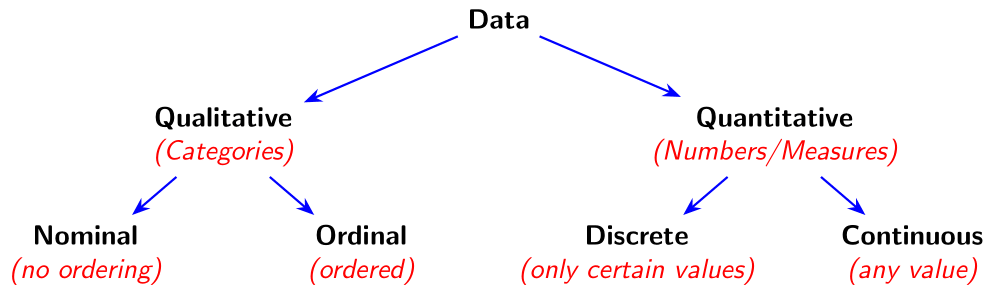
\includegraphics[keepaspectratio]{images/L1-Data-Decision-Tree.png}}
\end{center}

\begin{itemize}
\tightlist
\item
  Understand the basics of what data looks like.
\item
  Learn how to interpret p-values and confidence intervals.
\item
  Apply regression in R to a real dataset.
\end{itemize}

\bookmarksetup{startatroot}

\chapter{Data Detectives}\label{data-detectives}

One of the goals of this class is learning how to describe data and use
it to convey information about the variable of interest. To do this, we
will need to discuss some basic statistical formulas that we will use
throughout the semester. We will need to learn ``how to do'' the math in
this section, but we should also put an emphasis on the meaning of each
term and what it is telling us. Later on in this course, we will be able
to calculate all of these formulas using computer software, but we will
still need to know what the results are telling us.

\section{Describing the Center}\label{describing-the-center}

It may seem odd, but there are multiple ways to describe the center of a
dataset. Sometimes we might want the center to describe the mathematical
mean (the average on a test was 83.5), other times we might want it to
describe the middle value (half of the students got above an 86 on the
test), and other times we might want to describe it as the value
occurring the most often (the most common grade on the test was an 89).
All of these are acceptable ways to discuss the center of a dataset, but
they still tell us very different things.

The first method we will discuss is probably something we are all
familiar with, and that is the \textbf{mean}. The mean is the average
value of the data set and is calculated by summing up all of the values
and dividing by the number of observations. Next, we have the
\textbf{median}, which is the middle value in the data set where half of
the values are below it and half of the values are above it. To
calculate the median we will order the observations from smallest to
largest and then choose the middle observation. If there is an even
number of observations then a middle value will not be present and you
will need to take the mean of the middle two values to calculate the
median. Finally, we have the \textbf{mode}. This is the value that
occurs most often and is found by choosing the one that has the highest
frequency. There may be no mode, one mode, or multiple modes depending
on the dataset.

Below is an example of how we can calculate the center of the dataset
using the three terms above. The data describes the average game
attendance for the 11 basketball teams in the Metro Atlantic Athletic
Conference for the 2022-2023 competition year.

\begin{longtable}[]{@{}ll@{}}
\toprule\noalign{}
College & Average Basketball Attendance \\
\midrule\noalign{}
\endhead
\bottomrule\noalign{}
\endlastfoot
Canisius & 847 \\
Fairfield & 2,135 \\
Iona & 1,822 \\
Manhattan & 769 \\
Marist & 2,025 \\
Merrimack & 1,462 \\
Mount St.~Mary's & 1,888 \\
Niagara & 855 \\
Quinnipiac & 1,510 \\
Rider & 1,540 \\
Sacred Heart & 1,209 \\
Saint Peter's & 539 \\
Siena & 5,044 \\
\end{longtable}

XXXXXXXXXXXXXXXXXX INSERT PICTURE SHOWING MATH XXXXXXXXXXXXXXXXXX

We can notice that both the mean (1855.8) and the median (1289) tell us
very different stories about what the average attendance was at the
basketball games. One reason for this is because the mean is impacted by
extreme values, which we will call \textbf{outliers}. These are values
that are much smaller or larger than the rest of the dataset. For our
dataset, it appears that Siena is an outlier since their attendance is
much larger than the rest of the conference. If we were to temporarily
remove this value from the dataset the mean would drop to roughly 1400
while the median would only change slightly to 1163. Through this, we
can see that the mean is heavily influenced by outliers while the median
is relatively immune to them (the median changed a good amount in our
dataset since we have relatively few observations, if we had 100
different schools then we would not expect the median to be affected by
outliers).

\section{Describing the Spread}\label{describing-the-spread}

Another way to describe a dataset is to talk about the spread of the
data. Much like the center, this too can be done in several different
ways. The first way we can do this is by calculating the \textbf{range
difference} (often called the range). This takes the \textbf{maximum}
value (6415) and the \textbf{minimum} value (573) and subtracts them
from each other. This will give us a range difference (\textbf{max -
min}) of 5842, indicating the data is spread out over 5842 values.

An alternative way to discuss the spread of data is by calculating the
\textbf{standard deviation}. This is a measure that tells us how far
apart on average the values are from the mean. This calculation requires
a few steps, with the first being to calculate the mean of the data.
Second, you will need to calculate how far each value deviates from the
mean (that is the value - mean). Third you will need to square all of
the deviations, with the fourth step being adding up all of these
squared deviations. Finally, you will divide by the number of
observations minus 1 and then take the square root. While this sounds
complicated, it can be done by making a table. An example of this can be
seen below:

XXXXXXXXXXXXXXXXXX INSERT PICTURE SHOWING MATH XXXXXXXXXXXXXXXXXX

Looking at the example above, we can see that the data values are on
average 1638.5 away from the mean. Similar to the mean, the standard
deviation is also affected by outliers. If we were to temporarily remove
the outlier (Siena) then the standard deviation would drop to roughly
665. It is important to understand what the standard deviation is
telling us and the general method for calculating it, as the topic will
come up throughout this semester and your Data Science journey.

One of the many reasons why the standard deviation is important is
because it allows us to compare datasets that might have different
units. For instance, if we have a dataset describing heights and a
dataset describing weights then just talking about the range difference
or the standard deviation will not give us insight if one dataset is
more spread out than the other. What might be beneficial is discussing
the \textbf{standard deviation range difference}, as this is a
statistical term to calculate how many standard deviations the maximum
value differs from the minimum value. In our basketball attendance
example, the standard deviation range difference will be
\(\displaystyle \frac{5842}{1638.51}=3.57\). This tells us the data
falls over a range of 3.57 standard deviations.

\section{Calculating z-Score}\label{calculating-z-score}

Another useful technique to compare values is to determine how many
standard deviations away from the mean values are. This might help us
see if certain values are ``extremes''. To do this we will find the
\textbf{standard score} (also called the \textbf{z-score}) which is
calculated as:

\[\text{z-score}=\frac{\text{Observed} - \text{ Mean}}{\text{Standard Deviation}}\]

For our example, Mount St.~Mary's University has a z-score of \(0.04\)
while a school that has an average attendance of 900 spectators has a
z-score of \(-0.58\). Stating how far an observation is away from the
mean in terms of standard deviations helps give it more meaning.

\section{Visualizing the Data}\label{visualizing-the-data}

Visualizing data is also an important part of data science. We will
discuss many visualization techniques later in the semester, but we do
want to discuss a few big ones now. The first will be the
\textbf{histogram}, which will help us visualize quantitative data. With
this visualization, the height of the bar corresponds to how many
observations have values within the interval. We should note that the
bars are all touching each other since it is quantitative data. While
this visualization will help convey information about the data, it does
lose some of its detail due to the length of each category. In our
visualization below, colleges that have an average attendance of 1001
and 1999 are lumped into the same category when one is almost double the
other.

An additional technique that we will make use of throughout the semester
is the \textbf{density} plot, which can be thought of as a smoothing
curve for the histogram. It is more detailed than the histogram since it
can highlight certain spots where more or less data lie and it
alleviates some of the issues mentioned with histograms above. Below is
a visualization of both of these included. The
\texttt{red"\ line\ indicates\ the\ mean\ and\ the}blue'' line indicates
the median.

XXXXXXXXXXXXXXXXXX INSERT CODE FOR VISUALIZATIONS XXXXXXXXXXXXXXXXXX

We can also use visualizations to try and determine if relationships
exist between multiple variables. To do this we can use a
\textbf{scatter-plot}, which will plot one variable on the \(x\)-axis
and another variable on the \(y\)-axis. The points are plotted as
ordered pairs. In future classes we will investigate how to describe the
relationship of two variables using mathematics as well as learning how
to calculate the line of best fit. Our example has been tweaked a little
to include the student enrollment for each college in the conference. We
will plot these points to see if a relationship exists between game
attendance and student enrollment. We should stress though that just
because a relationship exists does not mean that one variable causes the
other variable to change. To quote the popular cliche:
\textbf{Correlation does not equal Causation!}

Based on our plot, it appears that as student enrollment increases
basketball attendance decreases. This does not make sense, as we would
probably expect schools with more students to have more fans at the
games. This may indicate that we are missing some other confounding
variable that is causing some confusion in our results (like population
of the surrounding area or even cost of attendance?).

XXXXXXXXXXXXXXXXXX INSERT CODE FOR VISUALIZATIONS XXXXXXXXXXXXXXXXXX

\section{Describing Qualitative Data}\label{describing-qualitative-data}

Everything we have discussed so far deals with quantitative data. We
cannot describe qualitative (categorical) data the same way though, as
it will not make sense to calculate and mean or the standard deviation
of groups. What we can do though is describe it using counts. The
example we have been using throughout this lecture is once again tweaked
to include a new column, the state where the University is located, and
whether or not the school is Catholic (C) or non-Catholic (NC).

XXXXXXXXXXXXXXXXXX INSERT CODE FOR VISUALIZATIONS XXXXXXXXXXXXXXXXXX

It is a relatively straightforward procedure, but we can do a
\textbf{count} by category and see that 8 schools are Catholic and 3
schools that are not Catholic. We could do something similar with their
locations and note that 6 schools are in New York, 2 are in Connecticut,
2 are in New Jersey, and 1 is in Maryland. To visualize categorical data
we can use a \textbf{barplot}. This is similar to the histogram but the
bars will not touch each other. Below is a visualization for both
counts:

XXXXXXXXXXXXXXXXXX INSERT CODE FOR VISUALIZATIONS XXXXXXXXXXXXXXXXXX

We can do a ``more exciting'' analysis with categorical data by
calculating quantitative descriptions within their categorical groups.
For instance, we could calculate the mean attendance for Catholic
schools (2069.88) and compare it to the mean attendance for non-Catholic
schools (1285). We could also do something similar for the school's
location:

XXXXXXXXXXXXXXXXXX INSERT CODE FOR VISUALIZATIONS XXXXXXXXXXXXXXXXXX

\bookmarksetup{startatroot}

\chapter{R Basics}\label{r-basics}

As Data Scientists, we will not have to calculate everything by hand,
but rather we will rely on a statistical programming language called R.
This is an open-source language (meaning anyone can contribute to it)
designed to clean, analyze, and present data. Before you begin coding in
R you should note that syntax rules do apply and it is an interpreted
language (meaning you can run it line by line). One of the benefits of R
(and why we are learning it) is that it is a popular, powerful, and
flexible language used by Data Scientists throughout the industry.

\section{The R Language}\label{the-r-language}

The language is maintained by the Comprehensive R Archive Network (CRAN)
and can be downloaded from their website
(\url{https://cran.r-project.org}). Since R is an open-source language,
community members can write their own programs and submit them to CRAN
for the whole community to use. Because of this, R is constantly
evolving and you can almost always find a library or a package that will
do the analysis you need it to do. If you have not already downloaded R
to your device then I would recommend doing so now so that you can
follow along with the rest of this lecture. A picture of the R console
can be seen below:

\begin{center}
\pandocbounded{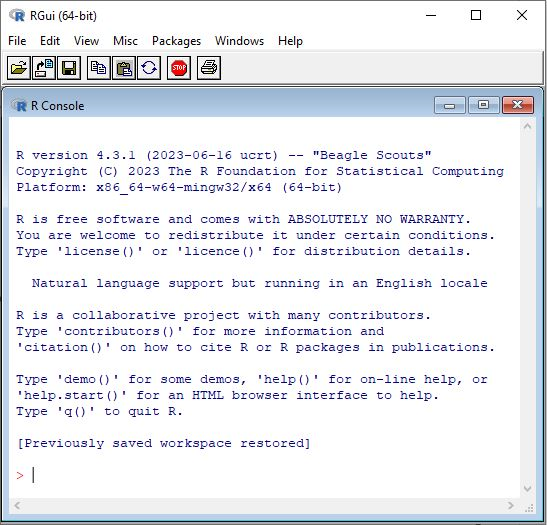
\includegraphics[keepaspectratio]{images/L3-R-console.png}}
\end{center}

\begin{watch}{}{}
    \href{https://youtu.be/TP9KX50x6a0}{Downloading and Installing R}
\end{watch}

Just because we can run all types of analysis on a dataset does not mean
that we should though, as you will not use all of the ingredients in
your pantry when you make dinner just because they are available to you.
You need to understand \textbf{what you are doing} when you run code or
analyze datasets. You should know what your dataset contains and the
different data types that you have. You should know the quality of your
data and if there are any underlying problems with the dataset, and you
should know if any relationships might exist within the dataset.

Knowing all of these things will not only help us in writing code to
analyze the data, but it will make our lives easier and save us time. A
famous phrase (possibly coined by Army specialist William Mellin) tells
us ``Garbage in\ldots{} Garbage out''. He expanded on this phrase with
the following explanation: ``If the problem has been sloppily programmed
the answer will be just as incorrect. If the programmer made mistakes
the machine will make mistakes. It can't correct them because it can't
do one thing: It can't think for itself.''

\section{Starting to Code}\label{starting-to-code}

The R Console will be where we will ``submit'' our code to be run line
by line. Any code you wish to run should be placed after the
\textgreater{} symbol. Let's open up R and type in \emph{Hello R} and
see what happens. We should get an error telling us that there is an
unexpected symbol present. This is because R does not understand what
the word \emph{Hello} means. If we want to type in
characters/words/strings then we need to do so inside of quotation marks
(either ``double'' quotes or `single' quotes). Below is an example of
what your results may look like. Note that for the rest of this course,
I will use the green box to represent the R console to display the
code/output.

\begin{Shaded}
\begin{Highlighting}[]
\NormalTok{Hello R}
\end{Highlighting}
\end{Shaded}

{Error: unexpected symbol in "Hello R"}

\begin{Shaded}
\begin{Highlighting}[]
\StringTok{"Hello R"}
\end{Highlighting}
\end{Shaded}

\begin{verbatim}
[1] "Hello R"
\end{verbatim}

\begin{Shaded}
\begin{Highlighting}[]
\StringTok{\textquotesingle{}Hello R\textquotesingle{}}
\end{Highlighting}
\end{Shaded}

\begin{verbatim}
[1] "Hello R"
\end{verbatim}

Before we continue running code in R, it is important to go over some
quick housekeeping notes. To begin, you will place your code after the
\textgreater. If you see a + on the left-hand side, it means that R is
expecting something more to end the previous line (maybe you are missing
a quotation mark or parenthesis). Anything you put after \# will be
considered a comment and nothing on the line after \# will run. It is
also important to realize that R is case sensitive so Mydata and mydata
are different. If you ever would like to access any previous commands
then you have them re-appear using the up and down arrows on your
keyboard. Finally, if you are ever unsure about the exact command syntax
then R will help you finish typing the commands (tab completion).

\begin{Shaded}
\begin{Highlighting}[]
\SpecialCharTok{\textgreater{}} \StringTok{"I am Dr. McCurdy}
\StringTok{+ and I forgot a quotation mark"}
\end{Highlighting}
\end{Shaded}

\begin{verbatim}
[1] "I am Dr. McCurdy\nand I forgot a quotation mark"
\end{verbatim}

\begin{Shaded}
\begin{Highlighting}[]
\CommentTok{\# Words after the pound sign will not run since it is a comment}
\DecValTok{2} \SpecialCharTok{+} \DecValTok{3} \CommentTok{\# Adding 2 numbers together}
\end{Highlighting}
\end{Shaded}

\begin{verbatim}
[1] 5
\end{verbatim}

\begin{watch}{}{}
    \href{https://youtu.be/Wf7Qwbr9Nko}{Starting to Code with R}
\end{watch}

\section{Understanding Error
Messages}\label{understanding-error-messages}

It is also probably time to discuss some of the things that can go wrong
when inputting code. The first that might occur (and the most obvious)
is a \textbf{syntax error}. This means that you have submitted invalid
code (maybe a forgotten comma, an ``open'' bracket, or misspelled a
function name/variable) and R returns an error message. It is important
to \textbf{read the error message}! About 95\% of the time it will be
easy to identify your mistake and fix it. We will see some common syntax
errors later on in the course as we get to new material.

Another error that you might make is a \textbf{semantic error}. This
occurs when your code is technically correct but it does not do what you
expected it to do. For instance, if you are trying to find the mean of a
dataset with 10 items and you divide by 11 instead, then R will run it
just fine, but you didn't calculate the mean. These semantic errors are
hard to find and figure out, but it does help to run your code
\textbf{line by line} to identify where the unexpected result occurs.
\textbf{When in doubt explain your code to a rubber duck!} (this means
that looking at your code line by line and trying to explain it usually
helps you identify the mistake)

\section{Using R as a Calculator}\label{using-r-as-a-calculator}

To get started with R, we should think of it as a calculator. Any
mathematical operations we wish to do we can. Below are a few examples
of the commands we can use:

\begin{Shaded}
\begin{Highlighting}[]
\CommentTok{\# Addition and Subtraction: use + and {-}}
\DecValTok{7} \SpecialCharTok{+} \DecValTok{3} \SpecialCharTok{{-}} \DecValTok{19} \SpecialCharTok{+} \DecValTok{8}
\end{Highlighting}
\end{Shaded}

\begin{verbatim}
[1] -1
\end{verbatim}

\begin{Shaded}
\begin{Highlighting}[]
\CommentTok{\# Multiplication and Division: use * and /}
\DecValTok{3} \SpecialCharTok{*} \DecValTok{8} \SpecialCharTok{/} \DecValTok{7}
\end{Highlighting}
\end{Shaded}

\begin{verbatim}
[1] 3.428571
\end{verbatim}

\begin{Shaded}
\begin{Highlighting}[]
\CommentTok{\# Exponentiation: use \^{}}
\DecValTok{4} \SpecialCharTok{\^{}} \DecValTok{5}
\end{Highlighting}
\end{Shaded}

\begin{verbatim}
[1] 1024
\end{verbatim}

\begin{Shaded}
\begin{Highlighting}[]
\CommentTok{\# Parenthesis for grouping calculated expressions: use ()}
\NormalTok{(}\DecValTok{3} \SpecialCharTok{+} \DecValTok{5}\NormalTok{)}\SpecialCharTok{/}\DecValTok{3}
\end{Highlighting}
\end{Shaded}

\begin{verbatim}
[1] 2.666667
\end{verbatim}

\begin{Shaded}
\begin{Highlighting}[]
\CommentTok{\# Integer Division (floor): use \%/\%}
\DecValTok{18} \SpecialCharTok{\%/\%} \DecValTok{7}
\end{Highlighting}
\end{Shaded}

\begin{verbatim}
[1] 2
\end{verbatim}

\begin{Shaded}
\begin{Highlighting}[]
\CommentTok{\# Modulus (remainder): use \%\%}
\DecValTok{18} \SpecialCharTok{\%\%} \DecValTok{7}
\end{Highlighting}
\end{Shaded}

\begin{verbatim}
[1] 4
\end{verbatim}

\begin{Shaded}
\begin{Highlighting}[]
\CommentTok{\# Example showing how the floor and remainder function work:}
\DecValTok{18}\SpecialCharTok{/}\DecValTok{7}
\end{Highlighting}
\end{Shaded}

\begin{verbatim}
[1] 2.571429
\end{verbatim}

\begin{Shaded}
\begin{Highlighting}[]
\DecValTok{18} \SpecialCharTok{\%/\%} \DecValTok{7} \SpecialCharTok{+} \DecValTok{18}\SpecialCharTok{\%\%}\DecValTok{7} \SpecialCharTok{/} \DecValTok{7}
\end{Highlighting}
\end{Shaded}

\begin{verbatim}
[1] 2.571429
\end{verbatim}

R follows the standard Order of Operations, with the order going
P-E-\%-MD-AS. This means that R will always carry out items in the
\textbf{Parenthesis} before going on to things outside of the
parenthesis. Next, R will look for \textbf{Exponentiation}, with the
operations being carried out from right to left. This means that
\(2 \wedge 2 \wedge 3\) is not \(4 \wedge 3\) but rather \(2\wedge8\).
Any special function indicated with a \% will be next. Then
\textbf{Multiplication} and \textbf{Division} are evaluated left to
right (which is typical) with \textbf{Addition} and \textbf{Subtraction}
being evaluated last (also left to right). It may take some getting used
to, so I always recommend putting more parenthesis than is required so
that you can have peace of mind that the calculation is what you
intended it to be.

As a practice, I encourage you to try evaluating the following
mathematical expressions. When doing so make sure that you use
parenthesis to group operations together. It is better to use too many
parentheses while we are learning the language instead of trying to
write a minimal solution.

For values that contain a certain number of significant figures (usually
more than 7), R will represent the results in scientific notation. This
is represented with an \(e\), which stands for \(\times 10^n\). For
instance, \(3.21\times 10^{-7}\) is represented in R as \(3.21e-7\).

\begin{Shaded}
\begin{Highlighting}[]
\DecValTok{102938303820387203828373}
\end{Highlighting}
\end{Shaded}

\begin{verbatim}
[1] 1.029383e+23
\end{verbatim}

\begin{Shaded}
\begin{Highlighting}[]
\NormalTok{.}\DecValTok{00000002828}
\end{Highlighting}
\end{Shaded}

\begin{verbatim}
[1] 2.828e-08
\end{verbatim}

\begin{Shaded}
\begin{Highlighting}[]
\FloatTok{2.31e{-}2}
\end{Highlighting}
\end{Shaded}

\begin{verbatim}
[1] 0.0231
\end{verbatim}

\begin{Shaded}
\begin{Highlighting}[]
\FloatTok{3.9282e12}
\end{Highlighting}
\end{Shaded}

\begin{verbatim}
[1] 3.9282e+12
\end{verbatim}

\section{Variables}\label{variables}

In addition to using R as a calculator, we can also save values as
\textbf{variables}. Variables will allow us to provide a reference (a
name) so that we can reuse the value later. To create a variable we will
use the \(<\)- operator (also called the assignment operator) with the
value we want to save ``pointing'' at the variable name. Like everything
else in R, variables are case-sensitive so we should make them short and
meaningful so that they are easy to type in over and over. We will be
able to name them anything we want, as the names can contain letters,
numbers, periods, or even underscores.

\begin{Shaded}
\begin{Highlighting}[]
\NormalTok{value1 }\OtherTok{\textless{}{-}} \DecValTok{3}
\NormalTok{value2 }\OtherTok{\textless{}{-}} \DecValTok{5}
\NormalTok{value1}
\end{Highlighting}
\end{Shaded}

\begin{verbatim}
[1] 3
\end{verbatim}

\begin{Shaded}
\begin{Highlighting}[]
\NormalTok{value1 }\SpecialCharTok{+}\NormalTok{ value2}
\end{Highlighting}
\end{Shaded}

\begin{verbatim}
[1] 8
\end{verbatim}

\begin{Shaded}
\begin{Highlighting}[]
\NormalTok{value3 }\CommentTok{\# will have a syntax error since value3 does not exist}
\end{Highlighting}
\end{Shaded}

{Error: object \textquotesingle value3\textquotesingle{} not found}

\begin{Shaded}
\begin{Highlighting}[]
\NormalTok{value3 }\OtherTok{\textless{}{-}}\NormalTok{ value1}\SpecialCharTok{*}\NormalTok{value2}
\NormalTok{value3}
\end{Highlighting}
\end{Shaded}

\begin{verbatim}
[1] 15
\end{verbatim}

These variables will allow us to save results for later use. If we
anticipate having to type in a calculation multiple times then we might
as well create a variable (type once; use often). It should be mentioned
that some variable names are ``off-limit'', such as the name of R
functions and commands. We will discuss that later in more detail
though.

\begin{Shaded}
\begin{Highlighting}[]
\NormalTok{x }\OtherTok{\textless{}{-}} \DecValTok{1}\SpecialCharTok{*}\DecValTok{2} \SpecialCharTok{+} \DecValTok{3}\SpecialCharTok{*}\DecValTok{4} \SpecialCharTok{+} \DecValTok{5}\SpecialCharTok{*}\DecValTok{6} \SpecialCharTok{+} \DecValTok{7}\SpecialCharTok{*}\DecValTok{8}
\NormalTok{y }\OtherTok{\textless{}{-}} \DecValTok{9}\SpecialCharTok{\^{}}\DecValTok{3} \SpecialCharTok{+} \DecValTok{8}\SpecialCharTok{\^{}}\DecValTok{3}
\NormalTok{z }\OtherTok{\textless{}{-}}\NormalTok{ (}\DecValTok{5} \SpecialCharTok{+} \DecValTok{3}\SpecialCharTok{\^{}}\DecValTok{2}\NormalTok{) }\SpecialCharTok{\^{}}\DecValTok{2}

\NormalTok{x }\SpecialCharTok{*}\NormalTok{ y}
\end{Highlighting}
\end{Shaded}

\begin{verbatim}
[1] 124100
\end{verbatim}

\begin{Shaded}
\begin{Highlighting}[]
\NormalTok{y }\SpecialCharTok{/}\NormalTok{ z}
\end{Highlighting}
\end{Shaded}

\begin{verbatim}
[1] 6.331633
\end{verbatim}

\section{The R Environment}\label{the-r-environment}

We interact with R through environments. Think of it as filing cabinets.
If we define a variable called x in one drawer (let's call it Drawer 1),
then when we open up Drawer 2 we will not be able to find x. This is
because it is not in Drawer 2, it is in Drawer 1. This is known as a
workspace, and most of the time we will be defining variables in the
global environment, so we will not have to worry about different
drawers. But, any variable that we initialize in R will remain in R as
long as our session is still active. We can see what variables and
objects currently exist in our environment with the \emph{ls()}
function.

\begin{Shaded}
\begin{Highlighting}[]
\FunctionTok{ls}\NormalTok{()}
\end{Highlighting}
\end{Shaded}

\begin{verbatim}
[1] "value1" "value2" "value3" "x"      "y"      "z"     
\end{verbatim}

\begin{Shaded}
\begin{Highlighting}[]
\FunctionTok{ls}\NormalTok{(}\AttributeTok{pattern=}\StringTok{"\^{}val"}\NormalTok{) }\CommentTok{\# can search for certain patterns}
\end{Highlighting}
\end{Shaded}

\begin{verbatim}
[1] "value1" "value2" "value3"
\end{verbatim}

If we ever need to remove a specific object in R from our workspace then
we can do this with the \emph{rm()} function. We should be careful with
this though, as we cannot reverse the removal of a variable. If we need
to clear our whole workspace then we can remove all objects with
\emph{rm(list=ls())}.

\begin{Shaded}
\begin{Highlighting}[]
\NormalTok{x}
\end{Highlighting}
\end{Shaded}

\begin{verbatim}
[1] 100
\end{verbatim}

\begin{Shaded}
\begin{Highlighting}[]
\FunctionTok{rm}\NormalTok{(x)}
\end{Highlighting}
\end{Shaded}

\begin{Shaded}
\begin{Highlighting}[]
\NormalTok{x}
\end{Highlighting}
\end{Shaded}

{Error: object \textquotesingle x\textquotesingle{} not found}

If you need to close R then you can either close it by using the command
\emph{q()} or by just exiting the window. When you close R it will ask
you if you want to ``Save workspace image?''. What this is asking is if
you would like to save all of your current objects in R (all of the
variables and functions you have made) and have them available to you in
your future R sessions. If you select yes then it will be saved under
your current directory under the file .RData. Most things we will be
doing in this class will not need to be saved in this manner as it will
be easy to recreate everything quickly if we do need something again.

\bookmarksetup{startatroot}

\chapter{Vectors and Factors in R}\label{vectors-and-factors-in-r}

\section{Data Types in R}\label{data-types-in-r}

So far we have seen how we can create variables in R. It is important to
note that all objects in R have a type (the big three are
\textbf{Doubles}, \textbf{Characters}, and \textbf{Logical}). A benefit
to R is that we do not have to declare each variable and type, as it can
figure all of that information out without us needing to do anything.
Doubles consist of our numbers, which can be integers or decimal values.
This is not the same as \emph{floating point} values in other languages
though. We can coerce the value to be an integer by placing an ``L''
after it (but there is no real benefit right now for integers over
doubles so don't worry about it). Characters will be anything in quotes,
whether it is a single letter, a word, a paragraph, a symbol, or a
number. R will treat all characters the same. The last type we should
discuss is the Logical type, which consists of TRUE and FALSE (yes it
has to be in all caps) or the shortened T and F. If we are ever unsure
of the type we are dealing with, we can use the \emph{typeof()} function
and R will tell us.

\begin{Shaded}
\begin{Highlighting}[]
\FunctionTok{typeof}\NormalTok{(}\FloatTok{17.2}\NormalTok{)}
\end{Highlighting}
\end{Shaded}

\begin{verbatim}
[1] "double"
\end{verbatim}

\begin{Shaded}
\begin{Highlighting}[]
\FunctionTok{typeof}\NormalTok{(}\DecValTok{17}\NormalTok{L)}
\end{Highlighting}
\end{Shaded}

\begin{verbatim}
[1] "integer"
\end{verbatim}

\begin{Shaded}
\begin{Highlighting}[]
\FunctionTok{typeof}\NormalTok{(}\DecValTok{17}\NormalTok{)}
\end{Highlighting}
\end{Shaded}

\begin{verbatim}
[1] "double"
\end{verbatim}

\begin{Shaded}
\begin{Highlighting}[]
\FunctionTok{typeof}\NormalTok{(}\StringTok{"17"}\NormalTok{)}
\end{Highlighting}
\end{Shaded}

\begin{verbatim}
[1] "character"
\end{verbatim}

\begin{Shaded}
\begin{Highlighting}[]
\FunctionTok{typeof}\NormalTok{(}\ConstantTok{TRUE}\NormalTok{)}
\end{Highlighting}
\end{Shaded}

\begin{verbatim}
[1] "logical"
\end{verbatim}

It is critical to know what type our value is as it will determine what
functions we can use, how we compose expressions, and how we will
interpret the results. For instance, we cannot do ``math'' on characters
but we can do ``math'' with doubles and logicals (though it might not
always make sense to do this).

\begin{Shaded}
\begin{Highlighting}[]
\StringTok{"a"} \SpecialCharTok{+} \StringTok{"b"}
\end{Highlighting}
\end{Shaded}

{Error in "a" + "b" : non-numeric argument to binary operator}

\begin{Shaded}
\begin{Highlighting}[]
\DecValTok{3} \SpecialCharTok{+} \ConstantTok{TRUE} \CommentTok{\# TRUE is equal to 1 and FALSE is equal to 0}
\end{Highlighting}
\end{Shaded}

\begin{verbatim}
[1] 4
\end{verbatim}

\begin{Shaded}
\begin{Highlighting}[]
\StringTok{"abc"} \SpecialCharTok{+} \DecValTok{2}
\end{Highlighting}
\end{Shaded}

{Error in "abc" + 2 : non-numeric argument to binary operator}

One thing that makes R different then some other languages is that R is
``vectorized'' (meaning everything is a vector). This characteristic
will allow us to quickly work with entire sets of data and avoids the
need for iterations or loops (but the \emph{for} and \emph{while} loop
still exist). So remember, \textbf{Everything is a Vector!!!}

\begin{watch}{}{}
    \href{https://youtu.be/6m-hh-NG0X0}{Data Types in R}
\end{watch}

\section{Vectors}\label{vectors}

To create a vector containing multiple elements we will use the combine
function \(c()\). This will allow us to combine multiple single-element
vectors into a multi-element vector. An example of this process can be
seen below:

\begin{Shaded}
\begin{Highlighting}[]
\NormalTok{x }\OtherTok{\textless{}{-}} \FunctionTok{c}\NormalTok{(}\DecValTok{1}\NormalTok{,}\DecValTok{2}\NormalTok{,}\DecValTok{3}\NormalTok{,}\DecValTok{4}\NormalTok{)}
\NormalTok{x}
\end{Highlighting}
\end{Shaded}

\begin{verbatim}
[1] 1 2 3 4
\end{verbatim}

\begin{Shaded}
\begin{Highlighting}[]
\NormalTok{y }\OtherTok{\textless{}{-}} \FunctionTok{c}\NormalTok{(}\StringTok{"Hello"}\NormalTok{, }\StringTok{"my name is"}\NormalTok{, }\StringTok{"Dr. McCurdy"}\NormalTok{)}
\NormalTok{y}
\end{Highlighting}
\end{Shaded}

\begin{verbatim}
[1] "Hello"       "my name is"  "Dr. McCurdy"
\end{verbatim}

If we create a vector with multiple types of data in it then it reverts
to the ``lowest'' one present (character \(<\) double \(<\) logical).
So, if at least one character is present then all of the elements are
turned into characters, and if no characters are present but a double is
then all elements turn into doubles. We can see the type a vector is
using the \emph{class()} function.

\begin{Shaded}
\begin{Highlighting}[]
\NormalTok{x }\OtherTok{\textless{}{-}} \FunctionTok{c}\NormalTok{(}\DecValTok{1}\NormalTok{,}\DecValTok{2}\NormalTok{,}\StringTok{"3"}\NormalTok{,}\DecValTok{4}\NormalTok{,}\DecValTok{5}\NormalTok{) }\CommentTok{\# One character is present}
\FunctionTok{class}\NormalTok{(x)}
\end{Highlighting}
\end{Shaded}

\begin{verbatim}
[1] "character"
\end{verbatim}

\begin{Shaded}
\begin{Highlighting}[]
\NormalTok{x}
\end{Highlighting}
\end{Shaded}

\begin{verbatim}
[1] "1" "2" "3" "4" "5"
\end{verbatim}

\begin{Shaded}
\begin{Highlighting}[]
\NormalTok{y }\OtherTok{\textless{}{-}} \FunctionTok{c}\NormalTok{(}\DecValTok{1}\NormalTok{, }\DecValTok{2}\NormalTok{, }\ConstantTok{TRUE}\NormalTok{, }\DecValTok{4}\NormalTok{, }\DecValTok{5}\NormalTok{) }\CommentTok{\# TRUE is turned into a 1}
\FunctionTok{class}\NormalTok{(y)}
\end{Highlighting}
\end{Shaded}

\begin{verbatim}
[1] "numeric"
\end{verbatim}

\begin{Shaded}
\begin{Highlighting}[]
\NormalTok{y}
\end{Highlighting}
\end{Shaded}

\begin{verbatim}
[1] 1 2 1 4 5
\end{verbatim}

If we need to explicitly coerce a vector to be a certain type we can
(for the most part). It is the nature of vectors to apply functions on
every element, so using a function like \emph{as.numeric()} or
\emph{as.character()} will try and force all elements to become a
certain type.

\begin{Shaded}
\begin{Highlighting}[]
\NormalTok{x }\OtherTok{\textless{}{-}} \FunctionTok{as.numeric}\NormalTok{(}\FunctionTok{c}\NormalTok{(}\DecValTok{1}\NormalTok{,}\DecValTok{2}\NormalTok{,}\StringTok{"3"}\NormalTok{,}\DecValTok{4}\NormalTok{,}\DecValTok{5}\NormalTok{)) }\CommentTok{\# 3 is coerced into a number}
\FunctionTok{class}\NormalTok{(x)}
\end{Highlighting}
\end{Shaded}

\begin{verbatim}
[1] "numeric"
\end{verbatim}

\begin{Shaded}
\begin{Highlighting}[]
\NormalTok{x}
\end{Highlighting}
\end{Shaded}

\begin{verbatim}
[1] 1 2 3 4 5
\end{verbatim}

\begin{Shaded}
\begin{Highlighting}[]
\NormalTok{y }\OtherTok{\textless{}{-}} \FunctionTok{as.character}\NormalTok{(}\FunctionTok{c}\NormalTok{(}\DecValTok{1}\NormalTok{,}\DecValTok{2}\NormalTok{,}\DecValTok{3}\NormalTok{,}\DecValTok{4}\NormalTok{,}\DecValTok{5}\NormalTok{)) }\CommentTok{\# All items are coerced into characters}
\FunctionTok{class}\NormalTok{(y)}
\end{Highlighting}
\end{Shaded}

\begin{verbatim}
[1] "character"
\end{verbatim}

\begin{Shaded}
\begin{Highlighting}[]
\NormalTok{y}
\end{Highlighting}
\end{Shaded}

\begin{verbatim}
[1] "1" "2" "3" "4" "5"
\end{verbatim}

\begin{watch}{}{}
    \href{https://youtu.be/vhNnJbHhPzE}{Creating Vectors in R}
\end{watch}

Whenever we are dealing with vectors it is important to resist the urge
to fight the vector's nature. That is, don't try and overthink it or
make it more difficult for yourself, R was meant to handle vectors.
\textbf{All arithmetic operators can be used on vectors}. It will apply
the operation between comparable elements and will ``recycle'' the
shorter vector if needed.

\begin{Shaded}
\begin{Highlighting}[]
\NormalTok{x }\OtherTok{\textless{}{-}} \FunctionTok{c}\NormalTok{(}\DecValTok{1}\NormalTok{,}\DecValTok{2}\NormalTok{,}\DecValTok{3}\NormalTok{,}\DecValTok{4}\NormalTok{,}\DecValTok{5}\NormalTok{)}
\NormalTok{x}
\end{Highlighting}
\end{Shaded}

\begin{verbatim}
[1] 1 2 3 4 5
\end{verbatim}

\begin{Shaded}
\begin{Highlighting}[]
\NormalTok{x }\SpecialCharTok{+} \DecValTok{13}
\end{Highlighting}
\end{Shaded}

\begin{verbatim}
[1] 14 15 16 17 18
\end{verbatim}

\begin{Shaded}
\begin{Highlighting}[]
\NormalTok{x }\SpecialCharTok{*} \SpecialCharTok{{-}}\DecValTok{2}
\end{Highlighting}
\end{Shaded}

\begin{verbatim}
[1]  -2  -4  -6  -8 -10
\end{verbatim}

\begin{Shaded}
\begin{Highlighting}[]
\NormalTok{x }\OtherTok{\textless{}{-}} \FunctionTok{c}\NormalTok{(}\DecValTok{1}\NormalTok{,}\DecValTok{2}\NormalTok{,}\DecValTok{3}\NormalTok{)}
\NormalTok{y }\OtherTok{\textless{}{-}} \FunctionTok{c}\NormalTok{(}\DecValTok{5}\NormalTok{,}\DecValTok{6}\NormalTok{,}\DecValTok{7}\NormalTok{)}

\NormalTok{x }\SpecialCharTok{+}\NormalTok{ y}
\end{Highlighting}
\end{Shaded}

\begin{verbatim}
[1]  6  8 10
\end{verbatim}

\begin{Shaded}
\begin{Highlighting}[]
\NormalTok{x}\SpecialCharTok{\^{}}\NormalTok{y}
\end{Highlighting}
\end{Shaded}

\begin{verbatim}
[1]    1   64 2187
\end{verbatim}

\begin{Shaded}
\begin{Highlighting}[]
\NormalTok{x }\OtherTok{\textless{}{-}} \FunctionTok{c}\NormalTok{(}\DecValTok{1}\NormalTok{,}\DecValTok{2}\NormalTok{,}\DecValTok{3}\NormalTok{,}\DecValTok{4}\NormalTok{,}\DecValTok{5}\NormalTok{)}
\NormalTok{y }\OtherTok{\textless{}{-}} \FunctionTok{c}\NormalTok{(}\DecValTok{1}\NormalTok{,}\DecValTok{10}\NormalTok{,}\DecValTok{100}\NormalTok{)}
\NormalTok{x }\SpecialCharTok{+}\NormalTok{ y}
\end{Highlighting}
\end{Shaded}

\begin{verbatim}
Warning in x + y: longer object length is not a multiple of shorter object
length
\end{verbatim}

\begin{verbatim}
[1]   2  12 103   5  15
\end{verbatim}

We can also make vectors that are not numeric. These can be both
character strings or logical values.

\begin{Shaded}
\begin{Highlighting}[]
\NormalTok{x }\OtherTok{\textless{}{-}} \FunctionTok{c}\NormalTok{(}\StringTok{"this"}\NormalTok{, }\StringTok{"is"}\NormalTok{, }\StringTok{"a"}\NormalTok{, }\StringTok{"character vector!"}\NormalTok{)}
\NormalTok{x}
\end{Highlighting}
\end{Shaded}

\begin{verbatim}
[1] "this"              "is"                "a"                
[4] "character vector!"
\end{verbatim}

\begin{Shaded}
\begin{Highlighting}[]
\NormalTok{y }\OtherTok{\textless{}{-}} \StringTok{"this is also a character vector!"}
\NormalTok{y}
\end{Highlighting}
\end{Shaded}

\begin{verbatim}
[1] "this is also a character vector!"
\end{verbatim}

\begin{Shaded}
\begin{Highlighting}[]
\NormalTok{z }\OtherTok{\textless{}{-}} \FunctionTok{c}\NormalTok{(T, T, F, F, T, F, T)}
\NormalTok{z}
\end{Highlighting}
\end{Shaded}

\begin{verbatim}
[1]  TRUE  TRUE FALSE FALSE  TRUE FALSE  TRUE
\end{verbatim}

\begin{watch}{}{}
    \href{https://youtu.be/L58Xl50txa0}{Doing Math with Vectors}
\end{watch}

\section{Logical Operators}\label{logical-operators}

One of the most important things we do in this class (and we will
repeatedly do it throughout the semester) is using logical operators on
vectors. If we compare 2 vectors using logical operators, the result
will be a logical vector. There are a few big ones that we will need to
know, and they are pretty well known. For instance, \(<\) means less
than, \(>\) means greater than, \(<=\) means less than or equal, \(>=\)
means greater than or equal, \(==\) means equal (notice it is two equal
signs), and \(!=\) means not equal.

\begin{Shaded}
\begin{Highlighting}[]
\NormalTok{x }\OtherTok{\textless{}{-}} \FunctionTok{c}\NormalTok{(}\DecValTok{0}\NormalTok{, }\DecValTok{4}\NormalTok{, }\DecValTok{2}\NormalTok{, }\DecValTok{5}\NormalTok{, }\DecValTok{3}\NormalTok{, }\DecValTok{6}\NormalTok{)}
\NormalTok{x}
\end{Highlighting}
\end{Shaded}

\begin{verbatim}
[1] 0 4 2 5 3 6
\end{verbatim}

\begin{Shaded}
\begin{Highlighting}[]
\NormalTok{x }\SpecialCharTok{==} \DecValTok{3} \CommentTok{\# Checks each element to see if it is equal to 3}
\end{Highlighting}
\end{Shaded}

\begin{verbatim}
[1] FALSE FALSE FALSE FALSE  TRUE FALSE
\end{verbatim}

\begin{Shaded}
\begin{Highlighting}[]
\NormalTok{x }\SpecialCharTok{\textgreater{}} \DecValTok{4} \CommentTok{\# Checks each element to see if it is greater than 4}
\end{Highlighting}
\end{Shaded}

\begin{verbatim}
[1] FALSE FALSE FALSE  TRUE FALSE  TRUE
\end{verbatim}

\begin{watch}{}{}
    \href{https://youtu.be/IKVtf3-yO3k}{Logical Operators in R}
\end{watch}

\section{Built-in statistical
functions}\label{built-in-statistical-functions}

Within R, there are also built-in functions that will make our lives
easier. All of the functions in this section will require us to pass a
vector into it and it will output a vector of the same size or of size 1
or 2. The names for these functions resemble the function name that we
would say out loud.

\begin{Shaded}
\begin{Highlighting}[]
\FunctionTok{sqrt}\NormalTok{(}\DecValTok{182}\NormalTok{)}
\end{Highlighting}
\end{Shaded}

\begin{verbatim}
[1] 13.49074
\end{verbatim}

\begin{Shaded}
\begin{Highlighting}[]
\NormalTok{x }\OtherTok{\textless{}{-}} \FunctionTok{c}\NormalTok{(}\DecValTok{2}\NormalTok{,}\DecValTok{49}\NormalTok{,}\DecValTok{381}\NormalTok{)}
\FunctionTok{sqrt}\NormalTok{(x)}
\end{Highlighting}
\end{Shaded}

\begin{verbatim}
[1]  1.414214  7.000000 19.519221
\end{verbatim}

\begin{Shaded}
\begin{Highlighting}[]
\FunctionTok{log}\NormalTok{(x)}
\end{Highlighting}
\end{Shaded}

\begin{verbatim}
[1] 0.6931472 3.8918203 5.9427994
\end{verbatim}

There are also functions in R that will do all of the calculations we
did in the earlier lectures. Unfortunately, there is no function to
calculate the mode of a dataset. When working with these functions, it
is important to make sure we pass a vector into the functions. This is a
common error students make when they start off.

\begin{Shaded}
\begin{Highlighting}[]
\NormalTok{x }\OtherTok{\textless{}{-}} \FunctionTok{c}\NormalTok{(}\DecValTok{12}\NormalTok{, }\DecValTok{10}\NormalTok{, }\DecValTok{18}\NormalTok{, }\DecValTok{11}\NormalTok{, }\DecValTok{11}\NormalTok{, }\DecValTok{15}\NormalTok{, }\DecValTok{21}\NormalTok{)}

\FunctionTok{sum}\NormalTok{(x)}
\end{Highlighting}
\end{Shaded}

\begin{verbatim}
[1] 98
\end{verbatim}

\begin{Shaded}
\begin{Highlighting}[]
\FunctionTok{mean}\NormalTok{(x)}
\end{Highlighting}
\end{Shaded}

\begin{verbatim}
[1] 14
\end{verbatim}

\begin{Shaded}
\begin{Highlighting}[]
\FunctionTok{median}\NormalTok{(x)}
\end{Highlighting}
\end{Shaded}

\begin{verbatim}
[1] 12
\end{verbatim}

\begin{Shaded}
\begin{Highlighting}[]
\FunctionTok{sd}\NormalTok{(x)}
\end{Highlighting}
\end{Shaded}

\begin{verbatim}
[1] 4.163332
\end{verbatim}

We can determine how long a vector is using the \textit{length()}
function. We could then use this function along with the sum function to
calculate the mean of the dataset:

\begin{Shaded}
\begin{Highlighting}[]
\FunctionTok{length}\NormalTok{(}\DecValTok{4}\NormalTok{)}
\end{Highlighting}
\end{Shaded}

\begin{verbatim}
[1] 1
\end{verbatim}

\begin{Shaded}
\begin{Highlighting}[]
\FunctionTok{length}\NormalTok{(}\FunctionTok{c}\NormalTok{(}\DecValTok{4}\NormalTok{,}\DecValTok{8}\NormalTok{,}\DecValTok{2}\NormalTok{))}
\end{Highlighting}
\end{Shaded}

\begin{verbatim}
[1] 3
\end{verbatim}

\begin{Shaded}
\begin{Highlighting}[]
\FunctionTok{length}\NormalTok{(x)}
\end{Highlighting}
\end{Shaded}

\begin{verbatim}
[1] 7
\end{verbatim}

\begin{Shaded}
\begin{Highlighting}[]
\FunctionTok{sum}\NormalTok{(x)}\SpecialCharTok{/}\FunctionTok{length}\NormalTok{(x) }\CommentTok{\# Notice this is the mean we found above}
\end{Highlighting}
\end{Shaded}

\begin{verbatim}
[1] 14
\end{verbatim}

In addition to this, we can calculate the minimum, maximum, and range
difference of a vector. We say range difference since the \emph{range()}
function provides both the minimum and maximum value, while the
\emph{diff()} function gives us the difference between the two values:

\begin{Shaded}
\begin{Highlighting}[]
\NormalTok{x}
\end{Highlighting}
\end{Shaded}

\begin{verbatim}
[1] 12 10 18 11 11 15 21
\end{verbatim}

\begin{Shaded}
\begin{Highlighting}[]
\FunctionTok{sort}\NormalTok{(x)}
\end{Highlighting}
\end{Shaded}

\begin{verbatim}
[1] 10 11 11 12 15 18 21
\end{verbatim}

\begin{Shaded}
\begin{Highlighting}[]
\FunctionTok{min}\NormalTok{(x)}
\end{Highlighting}
\end{Shaded}

\begin{verbatim}
[1] 10
\end{verbatim}

\begin{Shaded}
\begin{Highlighting}[]
\FunctionTok{max}\NormalTok{(x)}
\end{Highlighting}
\end{Shaded}

\begin{verbatim}
[1] 21
\end{verbatim}

\begin{Shaded}
\begin{Highlighting}[]
\FunctionTok{range}\NormalTok{(x)}
\end{Highlighting}
\end{Shaded}

\begin{verbatim}
[1] 10 21
\end{verbatim}

\begin{Shaded}
\begin{Highlighting}[]
\FunctionTok{diff}\NormalTok{(}\FunctionTok{range}\NormalTok{(x))}
\end{Highlighting}
\end{Shaded}

\begin{verbatim}
[1] 11
\end{verbatim}

\begin{watch}{}{}
    \href{https://youtu.be/pwgSeoNjwPo}{Built-in Functions in R}
\end{watch}

\section{Indexing in R}\label{indexing-in-r}

The last big thing we want to mention about vectors is how the elements
are indexed. R starts indexing at 1 (this means the first element is
index 1, the second element is index 2, and so on) which is different
then other languages which start counting at 0. To access specific
values we can place the indices in brackets. I will often refer to these
as our ``Index-Selection'' brackets. We must pass a vector into our
index-selection brackets using the combine function \emph{c()} if we
have multiple elements that we want to display.

\begin{Shaded}
\begin{Highlighting}[]
\NormalTok{x}
\end{Highlighting}
\end{Shaded}

\begin{verbatim}
[1] 12 10 18 11 11 15 21
\end{verbatim}

\begin{Shaded}
\begin{Highlighting}[]
\NormalTok{x[}\DecValTok{2}\NormalTok{]}
\end{Highlighting}
\end{Shaded}

\begin{verbatim}
[1] 10
\end{verbatim}

\begin{Shaded}
\begin{Highlighting}[]
\NormalTok{x[}\FunctionTok{length}\NormalTok{(x)]}
\end{Highlighting}
\end{Shaded}

\begin{verbatim}
[1] 21
\end{verbatim}

\begin{Shaded}
\begin{Highlighting}[]
\NormalTok{x[}\FunctionTok{c}\NormalTok{(}\DecValTok{1}\NormalTok{,}\DecValTok{3}\NormalTok{,}\DecValTok{6}\NormalTok{)]}
\end{Highlighting}
\end{Shaded}

\begin{verbatim}
[1] 12 18 15
\end{verbatim}

\begin{watch}{}{}
    \href{https://youtu.be/isTXaMdsyfI}{Indexing in R}
\end{watch}

\section{Creating Factors in R}\label{creating-factors-in-r}

So far we have seen a couple of different types of data in R, including
numeric, logical, and character types. Another type that we will use
quite a bit are \textbf{factors}. Factors will allow us to represent
categorical data that fit in only a finite number of distinct
categories. These factors could either be words (like Small, Medium, or
Large) or numbers (like a house having 1, 2, or 3 bedrooms). R does some
things behind the scenes to make it efficient to store this qualitative
data, but the only thing we really need to know is that if we have
categorical data then we should probably save it as a factor using the
\emph{factor()} function.

Let's create a vector containing a random sample of ``Males'' and
``Females'' using the \emph{sample()} function. First, we should realize
that this is categorical data, so we will want to convert it to a
factor. We can then use the \emph{factor()} function to convert it to
categories. Notice how the levels are in alphabetical order.

\begin{Shaded}
\begin{Highlighting}[]
\NormalTok{x }\OtherTok{\textless{}{-}} \FunctionTok{sample}\NormalTok{(}\FunctionTok{c}\NormalTok{(}\StringTok{"Male"}\NormalTok{, }\StringTok{"Female"}\NormalTok{), }\DecValTok{7}\NormalTok{, }\AttributeTok{replace=}\ConstantTok{TRUE}\NormalTok{)}
\NormalTok{x}
\end{Highlighting}
\end{Shaded}

\begin{verbatim}
[1] "Male"   "Male"   "Female" "Male"   "Male"   "Male"   "Female"
\end{verbatim}

\begin{Shaded}
\begin{Highlighting}[]
\NormalTok{fx }\OtherTok{\textless{}{-}} \FunctionTok{factor}\NormalTok{(x)}
\NormalTok{fx}
\end{Highlighting}
\end{Shaded}

\begin{verbatim}
[1] Male   Male   Female Male   Male   Male   Female
Levels: Female Male
\end{verbatim}

We can also notice how the vector class and the element type are also
altered. We don't have to understand the ``behind-the-scenes''
happenings of why the element type is now an integer. But we should
emphasize though that the new vector is no longer a character vector,
rather it is a factor since it is categorical data.

\begin{Shaded}
\begin{Highlighting}[]
\FunctionTok{class}\NormalTok{(x)}
\end{Highlighting}
\end{Shaded}

\begin{verbatim}
[1] "character"
\end{verbatim}

\begin{Shaded}
\begin{Highlighting}[]
\FunctionTok{class}\NormalTok{(fx)}
\end{Highlighting}
\end{Shaded}

\begin{verbatim}
[1] "factor"
\end{verbatim}

\begin{Shaded}
\begin{Highlighting}[]
\FunctionTok{typeof}\NormalTok{(x)}
\end{Highlighting}
\end{Shaded}

\begin{verbatim}
[1] "character"
\end{verbatim}

\begin{Shaded}
\begin{Highlighting}[]
\FunctionTok{typeof}\NormalTok{(fx)}
\end{Highlighting}
\end{Shaded}

\begin{verbatim}
[1] "integer"
\end{verbatim}

\begin{watch}{}{}
    \href{https://youtu.be/UoPKvEKD9K4}{Creating Factors in R}
\end{watch}

\section{Dealing with Ordinal Data}\label{dealing-with-ordinal-data}

If we remember from our previous lectures, categorical data can fall
into two types: Nominal and Ordinal. Right now our \emph{factor()}
function is returning the values in a nominal form (meaning the factors
have no specific ordering) and thus we cannot compare values.

\begin{Shaded}
\begin{Highlighting}[]
\NormalTok{fx[}\DecValTok{1}\NormalTok{] }\SpecialCharTok{\textgreater{}}\NormalTok{ fx[}\DecValTok{2}\NormalTok{]}
\end{Highlighting}
\end{Shaded}

{Warning in Ops.factor(fx{[}1{]}, fx{[}2{]}) :
\textquotesingle\textgreater\textquotesingle{} not meaningful for
factors}

\begin{verbatim}
[1] NA
\end{verbatim}

If we want to create ordinal data in R then all we have to do is specify
the `ordered' argument to be TRUE. An example of this can be seen below,
but note that the levels are in alphabetical order by default.

\begin{Shaded}
\begin{Highlighting}[]
\NormalTok{y }\OtherTok{\textless{}{-}} \FunctionTok{sample}\NormalTok{(}\FunctionTok{c}\NormalTok{(}\StringTok{"Small"}\NormalTok{, }\StringTok{"Medium"}\NormalTok{, }\StringTok{"Large"}\NormalTok{), }\DecValTok{7}\NormalTok{, }\AttributeTok{replace=}\ConstantTok{TRUE}\NormalTok{)}
\NormalTok{y}
\end{Highlighting}
\end{Shaded}

\begin{verbatim}
[1] "Medium" "Small"  "Large"  "Medium" "Large"  "Large"  "Medium"
\end{verbatim}

\begin{Shaded}
\begin{Highlighting}[]
\NormalTok{fy }\OtherTok{\textless{}{-}} \FunctionTok{factor}\NormalTok{(y, }\AttributeTok{ordered=}\ConstantTok{TRUE}\NormalTok{)}
\NormalTok{fy}
\end{Highlighting}
\end{Shaded}

\begin{verbatim}
[1] Medium Small  Large  Medium Large  Large  Medium
Levels: Large < Medium < Small
\end{verbatim}

This is obviously not what we want. When we go to a restaurant and order
a side of fries, we expect the Large to be bigger than the Medium which
is bigger than the Small. To have the levels end up in the correct
order, we will want to use the `levels' argument and pass it a vector of
the correct ordering. When you do this, the spelling has to be the same
(even the capitalization) for R to recognize it. Now that we have an
ordered factor, we can compare values using logical operators.

\begin{Shaded}
\begin{Highlighting}[]
\NormalTok{fy }\OtherTok{\textless{}{-}} \FunctionTok{factor}\NormalTok{(y, }\AttributeTok{ordered=}\ConstantTok{TRUE}\NormalTok{, }\AttributeTok{levels=}\FunctionTok{c}\NormalTok{(}\StringTok{"Small"}\NormalTok{, }\StringTok{"Medium"}\NormalTok{, }\StringTok{"Large"}\NormalTok{))}
\NormalTok{fy}
\end{Highlighting}
\end{Shaded}

\begin{verbatim}
[1] Medium Small  Large  Medium Large  Large  Medium
Levels: Small < Medium < Large
\end{verbatim}

\begin{Shaded}
\begin{Highlighting}[]
\FunctionTok{class}\NormalTok{(fy)}
\end{Highlighting}
\end{Shaded}

\begin{verbatim}
[1] "ordered" "factor" 
\end{verbatim}

\begin{Shaded}
\begin{Highlighting}[]
\NormalTok{fy[}\DecValTok{1}\NormalTok{] }\SpecialCharTok{\textgreater{}}\NormalTok{ fy[}\DecValTok{2}\NormalTok{]}
\end{Highlighting}
\end{Shaded}

\begin{verbatim}
[1] TRUE
\end{verbatim}

Additionally, we can always see the possible categories an element can
have in the factor by using the \emph{levels()} function. Finally, if we
wish to change the levels then we can do so by assigning a new character
vector to the current levels of factor. Be careful with this, as we do
not want to pass in the order of the vector elements, rather we want to
pass in the order of the levels.

\begin{Shaded}
\begin{Highlighting}[]
\NormalTok{fy}
\end{Highlighting}
\end{Shaded}

\begin{verbatim}
[1] Medium Small  Large  Medium Large  Large  Medium
Levels: Small < Medium < Large
\end{verbatim}

\begin{Shaded}
\begin{Highlighting}[]
\FunctionTok{levels}\NormalTok{(fy)}
\end{Highlighting}
\end{Shaded}

\begin{verbatim}
[1] "Small"  "Medium" "Large" 
\end{verbatim}

\begin{Shaded}
\begin{Highlighting}[]
\FunctionTok{levels}\NormalTok{(fy) }\OtherTok{\textless{}{-}} \FunctionTok{c}\NormalTok{(}\StringTok{"mini"}\NormalTok{, }\StringTok{"regular"}\NormalTok{, }\StringTok{"huge"}\NormalTok{)}
\NormalTok{fy}
\end{Highlighting}
\end{Shaded}

\begin{verbatim}
[1] regular mini    huge    regular huge    huge    regular
Levels: mini < regular < huge
\end{verbatim}

\begin{watch}{}{}
    \href{https://youtu.be/_PfBPa3GQWM}{Dealing with Ordinal Data}
\end{watch}

\section{RStudio}\label{rstudio}

So far, we have been using the R Console (RGui) to run code. While this
is sufficient to run all of our R code, we are going to introduce a
program called RStudio. This is the most commonly used IDE (Integrated
Development Environment) for R which will allow us to be more organized
and better for trouble-shooting our code. It is maintained by Posit and
can be downloaded
\href{https://posit.co/download/rstudio-desktop/}{here}. Since you
already have R installed, you will only need to download the RStudio
Desktop. Once this is done it should look something like this:

\begin{center}
\pandocbounded{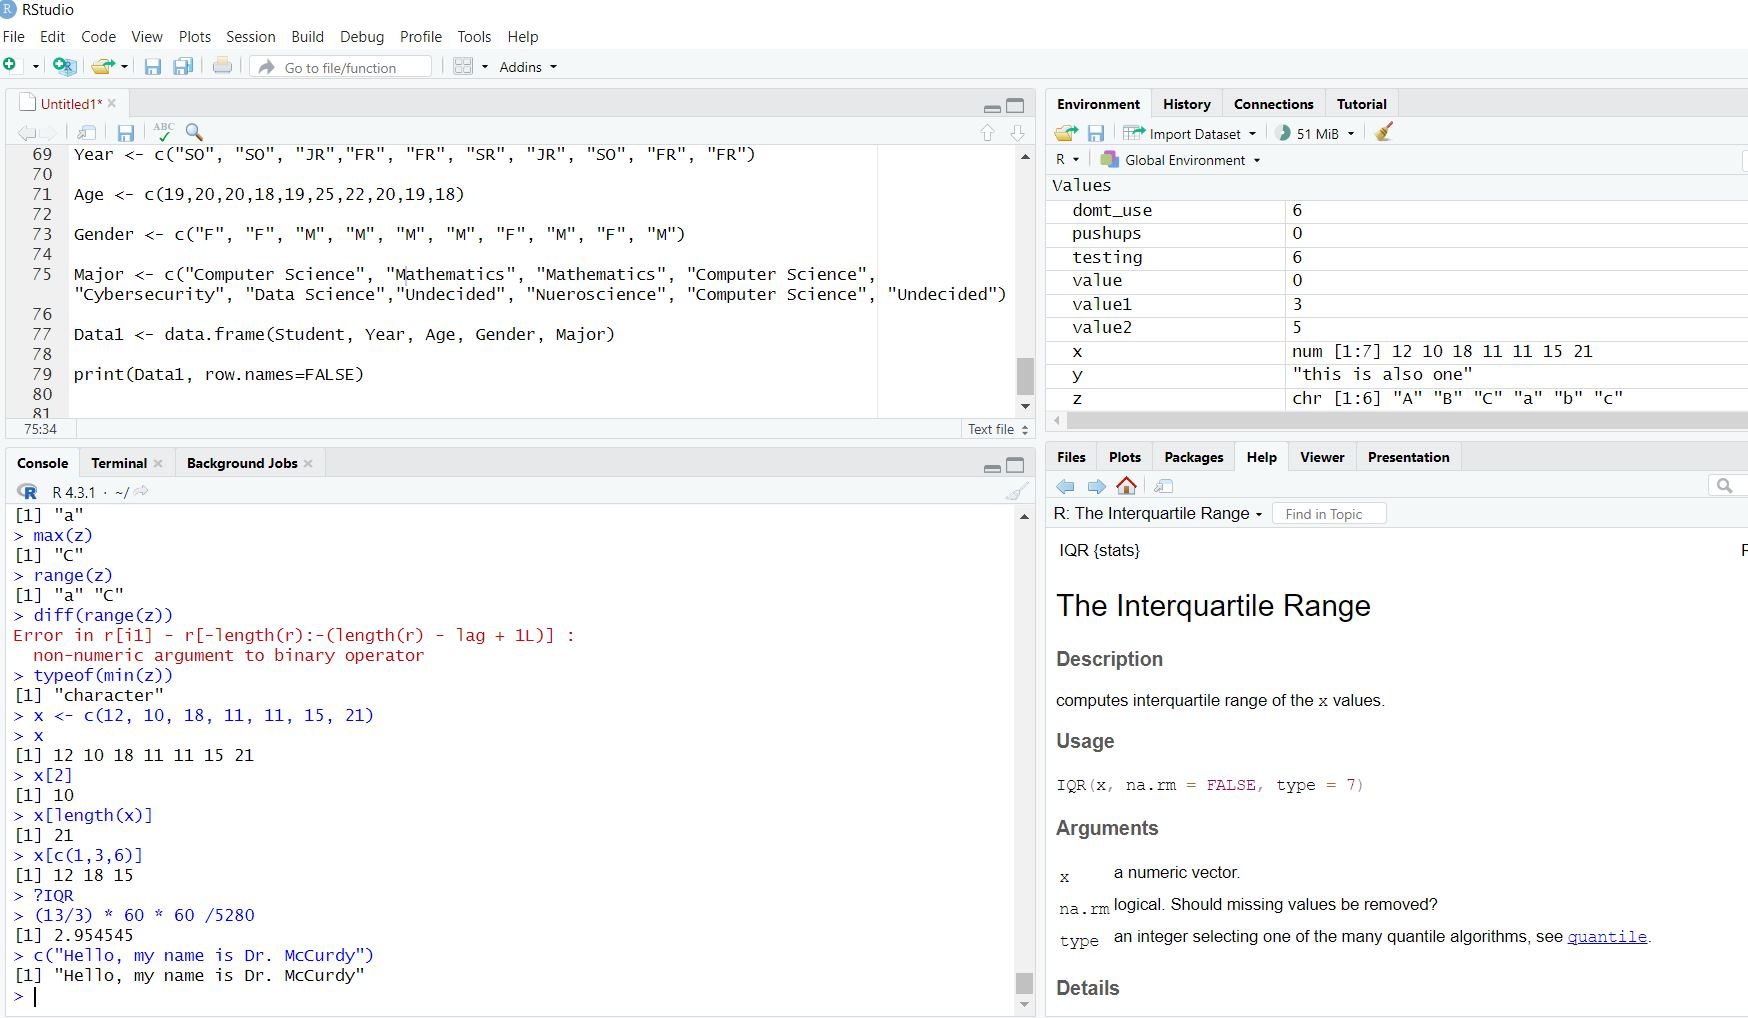
\includegraphics[keepaspectratio]{images/L4-RStudio-Download.png}}
\end{center}

We will run our code in the bottom left panel with the option to save
our code in the top left panel using a script or text file (more to come
on this in future lectures). In the top right panel we will be able to
see the variables saved in our R environment along with a history of our
code. In the bottom right panel we will be able to view plots, read
documentation, and browse files on our computer.

\bookmarksetup{startatroot}

\chapter{More R}\label{more-r}

So far we have seen the basics of R, including ways to use R as a
calculator as well as how to create variables and vectors. As a quick
reminder, we can create a vector containing multiple elements by using
our \emph{c()} function (which stands for combine). After creating a
vector we could then save it to a variable name by having the value
point towards the name of our variable. To do this, we will use the
assignment operator which looks like this: \(<\)--. An example of this
can be seen below:

\begin{Shaded}
\begin{Highlighting}[]
\NormalTok{x }\OtherTok{\textless{}{-}} \FunctionTok{c}\NormalTok{(}\DecValTok{1}\NormalTok{,}\DecValTok{2}\NormalTok{,}\DecValTok{3}\NormalTok{,}\DecValTok{4}\NormalTok{,}\DecValTok{5}\NormalTok{) }\CommentTok{\# Combining multiple elements into a single vector }
\NormalTok{x}
\end{Highlighting}
\end{Shaded}

\begin{verbatim}
[1] 1 2 3 4 5
\end{verbatim}

\begin{Shaded}
\begin{Highlighting}[]
\FunctionTok{c}\NormalTok{(}\StringTok{"Hello"}\NormalTok{, }\StringTok{"world!"}\NormalTok{) }\OtherTok{{-}\textgreater{}}\NormalTok{ y }\CommentTok{\# This also works but is not recommended}
\NormalTok{y}
\end{Highlighting}
\end{Shaded}

\begin{verbatim}
[1] "Hello"  "world!"
\end{verbatim}

\section{Creating a Sequence of
Numbers}\label{creating-a-sequence-of-numbers}

There are additional ways we could make a vector as well. If we wanted
all of our numbers in a sequence then we could use the \emph{seq()}
function to do this. With this function, we can specify what our
starting value is and what we want the sequence to do. The function also
allows us to pass an argument into it which specifies what value we
should increment the sequence by. If we do not specify what we should
increment by then it will automatically default to 1. We can also count
down if we would like. Finally, it should be mentioned that most
functions do not require us to write the argument name as long as we
pass them in the correct order (but we should probably keep doing it).

\begin{Shaded}
\begin{Highlighting}[]
\FunctionTok{seq}\NormalTok{(}\AttributeTok{from=}\DecValTok{1}\NormalTok{, }\AttributeTok{to=}\DecValTok{10}\NormalTok{)}
\end{Highlighting}
\end{Shaded}

\begin{verbatim}
 [1]  1  2  3  4  5  6  7  8  9 10
\end{verbatim}

\begin{Shaded}
\begin{Highlighting}[]
\FunctionTok{seq}\NormalTok{(}\AttributeTok{from=}\DecValTok{1}\NormalTok{, }\AttributeTok{to=}\DecValTok{10}\NormalTok{, }\AttributeTok{by=}\DecValTok{2}\NormalTok{)}
\end{Highlighting}
\end{Shaded}

\begin{verbatim}
[1] 1 3 5 7 9
\end{verbatim}

\begin{Shaded}
\begin{Highlighting}[]
\FunctionTok{seq}\NormalTok{(}\DecValTok{7}\NormalTok{, }\DecValTok{1}\NormalTok{)}
\end{Highlighting}
\end{Shaded}

\begin{verbatim}
[1] 7 6 5 4 3 2 1
\end{verbatim}

\begin{Shaded}
\begin{Highlighting}[]
\FunctionTok{seq}\NormalTok{(}\AttributeTok{from=}\DecValTok{30}\NormalTok{, }\AttributeTok{to=}\DecValTok{1}\NormalTok{, }\AttributeTok{by=}\SpecialCharTok{{-}}\DecValTok{4}\NormalTok{)}
\end{Highlighting}
\end{Shaded}

\begin{verbatim}
[1] 30 26 22 18 14 10  6  2
\end{verbatim}

\begin{Shaded}
\begin{Highlighting}[]
\FunctionTok{seq}\NormalTok{(}\SpecialCharTok{{-}}\DecValTok{1}\NormalTok{,}\DecValTok{2}\NormalTok{,}\AttributeTok{by=}\FloatTok{0.3}\NormalTok{)}
\end{Highlighting}
\end{Shaded}

\begin{verbatim}
 [1] -1.0 -0.7 -0.4 -0.1  0.2  0.5  0.8  1.1  1.4  1.7  2.0
\end{verbatim}

If we do not need to increment the sequence by a certain value then we
could do something similar with a colon. This will create a sequence by
just adding 1 to a value until it reaches the end number. An example of
this can be seen below:

\begin{Shaded}
\begin{Highlighting}[]
\DecValTok{1}\SpecialCharTok{:}\DecValTok{10}
\end{Highlighting}
\end{Shaded}

\begin{verbatim}
 [1]  1  2  3  4  5  6  7  8  9 10
\end{verbatim}

\begin{Shaded}
\begin{Highlighting}[]
\DecValTok{7}\SpecialCharTok{:{-}}\DecValTok{2}
\end{Highlighting}
\end{Shaded}

\begin{verbatim}
 [1]  7  6  5  4  3  2  1  0 -1 -2
\end{verbatim}

\begin{Shaded}
\begin{Highlighting}[]
\FloatTok{0.25}\SpecialCharTok{:}\FloatTok{7.75} \CommentTok{\# Notice how it does not go past the ending value}
\end{Highlighting}
\end{Shaded}

\begin{verbatim}
[1] 0.25 1.25 2.25 3.25 4.25 5.25 6.25 7.25
\end{verbatim}

\begin{watch}{}{}
    \href{https://youtu.be/c4qJ3Y5hJ0s}{Creating a Sequence of Numbers}
\end{watch}

\section{Replicating Values}\label{replicating-values}

We can replicate values (of any type) using the \emph{rep()} function.
This will allow us to pass a vector into the function and have it be
replicated a certain number of times (and the number of times could also
be a vector!). If we pass a vector in for the number of times then it
will match it element by element and replicate it the specified number
of times before going on to the next element.

\begin{Shaded}
\begin{Highlighting}[]
\FunctionTok{rep}\NormalTok{(}\DecValTok{2}\NormalTok{, }\AttributeTok{times=}\DecValTok{6}\NormalTok{)}
\end{Highlighting}
\end{Shaded}

\begin{verbatim}
[1] 2 2 2 2 2 2
\end{verbatim}

\begin{Shaded}
\begin{Highlighting}[]
\FunctionTok{rep}\NormalTok{(}\StringTok{"abc"}\NormalTok{, }\AttributeTok{times=}\DecValTok{3}\NormalTok{)}
\end{Highlighting}
\end{Shaded}

\begin{verbatim}
[1] "abc" "abc" "abc"
\end{verbatim}

\begin{Shaded}
\begin{Highlighting}[]
\FunctionTok{rep}\NormalTok{(}\DecValTok{1}\SpecialCharTok{:}\DecValTok{4}\NormalTok{, }\AttributeTok{times=}\DecValTok{4}\SpecialCharTok{:}\DecValTok{1}\NormalTok{) }\CommentTok{\# 1st element 4 times, 2nd element 3 times, etc.}
\end{Highlighting}
\end{Shaded}

\begin{verbatim}
 [1] 1 1 1 1 2 2 2 3 3 4
\end{verbatim}

\begin{Shaded}
\begin{Highlighting}[]
\FunctionTok{rep}\NormalTok{(}\FunctionTok{c}\NormalTok{(}\DecValTok{7}\NormalTok{,}\DecValTok{2}\NormalTok{,}\DecValTok{1}\NormalTok{), }\AttributeTok{times=}\FunctionTok{c}\NormalTok{(}\DecValTok{1}\NormalTok{,}\DecValTok{4}\NormalTok{,}\DecValTok{8}\NormalTok{))}
\end{Highlighting}
\end{Shaded}

\begin{verbatim}
 [1] 7 2 2 2 2 1 1 1 1 1 1 1 1
\end{verbatim}

The function allows for other arguments as well, such as the length of
the outputted sequence and if all of the elements should be replicated a
certain amount of times. The `each' argument will replicate each element
a certain number of times while the `length.out' argument will keep
repeating a sequence until it is of a certain length.

\begin{Shaded}
\begin{Highlighting}[]
\FunctionTok{rep}\NormalTok{(}\FunctionTok{c}\NormalTok{(}\DecValTok{7}\NormalTok{,}\DecValTok{2}\NormalTok{,}\DecValTok{1}\NormalTok{), }\AttributeTok{times=}\DecValTok{2}\NormalTok{)}
\end{Highlighting}
\end{Shaded}

\begin{verbatim}
[1] 7 2 1 7 2 1
\end{verbatim}

\begin{Shaded}
\begin{Highlighting}[]
\FunctionTok{rep}\NormalTok{(}\FunctionTok{c}\NormalTok{(}\DecValTok{7}\NormalTok{,}\DecValTok{2}\NormalTok{,}\DecValTok{1}\NormalTok{), }\AttributeTok{each=}\DecValTok{2}\NormalTok{)}
\end{Highlighting}
\end{Shaded}

\begin{verbatim}
[1] 7 7 2 2 1 1
\end{verbatim}

\begin{Shaded}
\begin{Highlighting}[]
\FunctionTok{rep}\NormalTok{(}\FunctionTok{c}\NormalTok{(}\DecValTok{7}\NormalTok{,}\DecValTok{2}\NormalTok{,}\DecValTok{1}\NormalTok{), }\AttributeTok{length.out =} \DecValTok{8}\NormalTok{)}
\end{Highlighting}
\end{Shaded}

\begin{verbatim}
[1] 7 2 1 7 2 1 7 2
\end{verbatim}

\begin{Shaded}
\begin{Highlighting}[]
\FunctionTok{rep}\NormalTok{(}\FunctionTok{c}\NormalTok{(}\DecValTok{7}\NormalTok{,}\DecValTok{2}\NormalTok{,}\DecValTok{1}\NormalTok{), }\AttributeTok{each=}\DecValTok{3}\NormalTok{, }\AttributeTok{length.out=}\DecValTok{10}\NormalTok{)}
\end{Highlighting}
\end{Shaded}

\begin{verbatim}
 [1] 7 7 7 2 2 2 1 1 1 7
\end{verbatim}

\begin{watch}{}{}
    \href{https://youtu.be/OGBhjbDChgQ}{Replicating Values}
\end{watch}

\section{Creating a Vector of
Letters}\label{creating-a-vector-of-letters}

As a quick reminder (since it is very important), R starts indexing at
1. This means that the first element in a vector is in the `1' index.
Other languages, like Python, start counting at 0 but we will start
counting at 1 in R. In R there is a vector called `letters' that
contains all of the lower-case letters. If we want to find out what the
4th letter is then we can use our ``index-selection'' brackets. We can
also pass a vector into the index selection brackets as well, which
includes sequences and replicated vectors (as long as they are numeric).
There is also a vector in R called `LETTERS' which acts the same way but
contains all capitalized letters.

\begin{Shaded}
\begin{Highlighting}[]
\NormalTok{x }\OtherTok{\textless{}{-}}\NormalTok{ letters }\CommentTok{\# Saving the vector to \textquotesingle{}x\textquotesingle{} for simplicity}
\NormalTok{x}
\end{Highlighting}
\end{Shaded}

\begin{verbatim}
 [1] "a" "b" "c" "d" "e" "f" "g" "h" "i" "j" "k" "l" "m" "n" "o" "p" "q" "r" "s"
[20] "t" "u" "v" "w" "x" "y" "z"
\end{verbatim}

\begin{Shaded}
\begin{Highlighting}[]
\NormalTok{x[}\FunctionTok{c}\NormalTok{(}\DecValTok{13}\NormalTok{, }\DecValTok{15}\NormalTok{, }\DecValTok{21}\NormalTok{, }\DecValTok{14}\NormalTok{, }\DecValTok{20}\NormalTok{)]}
\end{Highlighting}
\end{Shaded}

\begin{verbatim}
[1] "m" "o" "u" "n" "t"
\end{verbatim}

\begin{Shaded}
\begin{Highlighting}[]
\NormalTok{x[}\DecValTok{17}\SpecialCharTok{:}\DecValTok{22}\NormalTok{]}
\end{Highlighting}
\end{Shaded}

\begin{verbatim}
[1] "q" "r" "s" "t" "u" "v"
\end{verbatim}

\begin{Shaded}
\begin{Highlighting}[]
\NormalTok{LETTERS[}\FunctionTok{c}\NormalTok{(}\DecValTok{8}\NormalTok{, }\DecValTok{5}\NormalTok{, }\DecValTok{12}\NormalTok{, }\DecValTok{12}\NormalTok{, }\DecValTok{15}\NormalTok{)]}
\end{Highlighting}
\end{Shaded}

\begin{verbatim}
[1] "H" "E" "L" "L" "O"
\end{verbatim}

If we ever wish to have all of the values displayed \textbf{except for}
certain ones then we can put a negative in front of the value/vector and
it will display everything except those values. This is helpful when it
is easier to exclude certain indices instead of having to specify all of
the desired indices.

\begin{Shaded}
\begin{Highlighting}[]
\NormalTok{x[}\FunctionTok{seq}\NormalTok{(}\DecValTok{1}\NormalTok{,}\DecValTok{26}\NormalTok{,}\AttributeTok{by=}\DecValTok{2}\NormalTok{)] }\CommentTok{\# Every other letter}
\end{Highlighting}
\end{Shaded}

\begin{verbatim}
 [1] "a" "c" "e" "g" "i" "k" "m" "o" "q" "s" "u" "w" "y"
\end{verbatim}

\begin{Shaded}
\begin{Highlighting}[]
\NormalTok{x[}\SpecialCharTok{{-}}\FunctionTok{seq}\NormalTok{(}\DecValTok{1}\NormalTok{,}\DecValTok{26}\NormalTok{,}\AttributeTok{by=}\DecValTok{2}\NormalTok{)] }\CommentTok{\# Everything but these indices}
\end{Highlighting}
\end{Shaded}

\begin{verbatim}
 [1] "b" "d" "f" "h" "j" "l" "n" "p" "r" "t" "v" "x" "z"
\end{verbatim}

\begin{Shaded}
\begin{Highlighting}[]
\NormalTok{y }\OtherTok{\textless{}{-}} \DecValTok{1}\SpecialCharTok{:}\DecValTok{10}
\NormalTok{y}
\end{Highlighting}
\end{Shaded}

\begin{verbatim}
 [1]  1  2  3  4  5  6  7  8  9 10
\end{verbatim}

\begin{Shaded}
\begin{Highlighting}[]
\NormalTok{y[}\FunctionTok{c}\NormalTok{(}\DecValTok{1}\NormalTok{,}\DecValTok{5}\NormalTok{,}\DecValTok{8}\NormalTok{)]}
\end{Highlighting}
\end{Shaded}

\begin{verbatim}
[1] 1 5 8
\end{verbatim}

\begin{Shaded}
\begin{Highlighting}[]
\NormalTok{y[}\SpecialCharTok{{-}}\FunctionTok{c}\NormalTok{(}\DecValTok{1}\NormalTok{,}\DecValTok{5}\NormalTok{,}\DecValTok{8}\NormalTok{)]}
\end{Highlighting}
\end{Shaded}

\begin{verbatim}
[1]  2  3  4  6  7  9 10
\end{verbatim}

\begin{watch}{}{}
    \href{https://youtu.be/H-q_LZVM0_0}{Using the Letters Vector}
\end{watch}

\section{Named Vectors}\label{named-vectors}

Since we have been discussing vectors and their elements, we should go
ahead and mention that we can name the individual elements as well (this
might make it easier for us to refer back to a specific element as we
might not remember which index it is). There are a few different ways we
can do this, the first is by naming them when we create the vector
itself. To do this we will just put the name of the element to the left
of the element with an equals sign in between. It may look something
like this:

\begin{Shaded}
\begin{Highlighting}[]
\NormalTok{x }\OtherTok{\textless{}{-}} \FunctionTok{c}\NormalTok{(}\AttributeTok{M=}\StringTok{"Monday"}\NormalTok{, }\AttributeTok{W=}\StringTok{"Wednesday"}\NormalTok{, }\AttributeTok{F=}\StringTok{"Friday"}\NormalTok{)}
\NormalTok{x}
\end{Highlighting}
\end{Shaded}

\begin{verbatim}
          M           W           F 
   "Monday" "Wednesday"    "Friday" 
\end{verbatim}

\begin{Shaded}
\begin{Highlighting}[]
\FunctionTok{names}\NormalTok{(x)}
\end{Highlighting}
\end{Shaded}

\begin{verbatim}
[1] "M" "W" "F"
\end{verbatim}

Another way that might be beneficial is to name them after the vector
has been created using the \emph{names()} function. We will reference
the names function with the vector inside and we will assign a character
vector to it. This will update the names of the vector elements as
whatever we passed into it. An example of this can also be seen below:

\begin{Shaded}
\begin{Highlighting}[]
\NormalTok{x }\OtherTok{\textless{}{-}} \FunctionTok{c}\NormalTok{(}\StringTok{"Monday"}\NormalTok{, }\StringTok{"Wednesday"}\NormalTok{, }\StringTok{"Friday"}\NormalTok{)}
\FunctionTok{names}\NormalTok{(x)}
\end{Highlighting}
\end{Shaded}

\begin{verbatim}
NULL
\end{verbatim}

\begin{Shaded}
\begin{Highlighting}[]
\FunctionTok{names}\NormalTok{(x) }\OtherTok{\textless{}{-}} \FunctionTok{c}\NormalTok{(}\StringTok{"M"}\NormalTok{, }\StringTok{"W"}\NormalTok{, }\StringTok{"F"}\NormalTok{)}
\NormalTok{x}
\end{Highlighting}
\end{Shaded}

\begin{verbatim}
          M           W           F 
   "Monday" "Wednesday"    "Friday" 
\end{verbatim}

\begin{Shaded}
\begin{Highlighting}[]
\FunctionTok{names}\NormalTok{(x)}
\end{Highlighting}
\end{Shaded}

\begin{verbatim}
[1] "M" "W" "F"
\end{verbatim}

Because the elements are named, we can pass the names into our
index-selection brackets and R will output the element associated with
that particular name. We will also still be able to access them with the
index value as well.

\begin{Shaded}
\begin{Highlighting}[]
\NormalTok{x[}\StringTok{"M"}\NormalTok{]}
\end{Highlighting}
\end{Shaded}

\begin{verbatim}
       M 
"Monday" 
\end{verbatim}

\begin{Shaded}
\begin{Highlighting}[]
\NormalTok{x[}\FunctionTok{c}\NormalTok{(}\StringTok{"M"}\NormalTok{, }\StringTok{"F"}\NormalTok{)]}
\end{Highlighting}
\end{Shaded}

\begin{verbatim}
       M        F 
"Monday" "Friday" 
\end{verbatim}

\begin{Shaded}
\begin{Highlighting}[]
\NormalTok{x[}\FunctionTok{c}\NormalTok{(}\DecValTok{1}\NormalTok{,}\DecValTok{3}\NormalTok{)]}
\end{Highlighting}
\end{Shaded}

\begin{verbatim}
       M        F 
"Monday" "Friday" 
\end{verbatim}

\begin{watch}{}{}
    \href{https://youtu.be/uYHuPb60zSA}{Named Vectors}
\end{watch}

\section{Index Selection using GREP}\label{index-selection-using-grep}

One very powerful tool in R that allows us to search a string for a
specific pattern is the \emph{grep()} function. This stands for
Global/Regular Expression/Print and is important to us as it will allow
us to identify all of the elements containing a specific pattern. To see
this function in action we will utilize the ``euro'' vector which is a
named vector available to us in R.

\begin{Shaded}
\begin{Highlighting}[]
\NormalTok{euro}
\end{Highlighting}
\end{Shaded}

\begin{verbatim}
        ATS         BEF         DEM         ESP         FIM         FRF 
  13.760300   40.339900    1.955830  166.386000    5.945730    6.559570 
        IEP         ITL         LUF         NLG         PTE 
   0.787564 1936.270000   40.339900    2.203710  200.482000 
\end{verbatim}

Before we jump into using the function though, we will want to discuss
some of the syntax that the \emph{grep()} uses. The first is that it
expects us to pass a pattern into it using quotation marks. If we type a
\(\wedge\) at the beginning of the pattern then it will search for
strings \textbf{starting with} the pattern. If we type a \$ at the end
of the pattern then it will search for strings \textbf{ending with} the
pattern. A single period will stand for any character, and brackets
characters in brackets will mean ``any of these characters''. After we
specify the pattern we will need to also specify where we are looking
for the pattern, and in our case, it will be the names of the euro
vector. The output for this function will be the indices of the elements
which contain the specified pattern.

\begin{Shaded}
\begin{Highlighting}[]
\FunctionTok{names}\NormalTok{(euro)}
\end{Highlighting}
\end{Shaded}

\begin{verbatim}
 [1] "ATS" "BEF" "DEM" "ESP" "FIM" "FRF" "IEP" "ITL" "LUF" "NLG" "PTE"
\end{verbatim}

\begin{Shaded}
\begin{Highlighting}[]
\FunctionTok{grep}\NormalTok{(}\StringTok{"E"}\NormalTok{, }\FunctionTok{names}\NormalTok{(euro)) }\CommentTok{\# Indices of elements containing an E anywhere}
\end{Highlighting}
\end{Shaded}

\begin{verbatim}
[1]  2  3  4  7 11
\end{verbatim}

\begin{Shaded}
\begin{Highlighting}[]
\NormalTok{euro[}\FunctionTok{grep}\NormalTok{(}\StringTok{"E"}\NormalTok{, }\FunctionTok{names}\NormalTok{(euro))] }\CommentTok{\# Names containing an E anywhere}
\end{Highlighting}
\end{Shaded}

\begin{verbatim}
       BEF        DEM        ESP        IEP        PTE 
 40.339900   1.955830 166.386000   0.787564 200.482000 
\end{verbatim}

\begin{Shaded}
\begin{Highlighting}[]
\FunctionTok{grep}\NormalTok{(}\StringTok{"\^{}I"}\NormalTok{, }\FunctionTok{names}\NormalTok{(euro)) }\CommentTok{\# Indices of elements starting with I}
\end{Highlighting}
\end{Shaded}

\begin{verbatim}
[1] 7 8
\end{verbatim}

\begin{Shaded}
\begin{Highlighting}[]
\NormalTok{euro[}\FunctionTok{grep}\NormalTok{(}\StringTok{"\^{}I"}\NormalTok{, }\FunctionTok{names}\NormalTok{(euro))] }\CommentTok{\# Names starting with I}
\end{Highlighting}
\end{Shaded}

\begin{verbatim}
        IEP         ITL 
   0.787564 1936.270000 
\end{verbatim}

\begin{Shaded}
\begin{Highlighting}[]
\FunctionTok{grep}\NormalTok{(}\StringTok{"F$"}\NormalTok{, }\FunctionTok{names}\NormalTok{(euro)) }\CommentTok{\# Indices of elements ending with F}
\end{Highlighting}
\end{Shaded}

\begin{verbatim}
[1] 2 6 9
\end{verbatim}

\begin{Shaded}
\begin{Highlighting}[]
\NormalTok{euro[}\FunctionTok{grep}\NormalTok{(}\StringTok{"F$"}\NormalTok{, }\FunctionTok{names}\NormalTok{(euro))] }\CommentTok{\# Names ending with F}
\end{Highlighting}
\end{Shaded}

\begin{verbatim}
     BEF      FRF      LUF 
40.33990  6.55957 40.33990 
\end{verbatim}

\begin{Shaded}
\begin{Highlighting}[]
\FunctionTok{grep}\NormalTok{(}\StringTok{".E."}\NormalTok{, }\FunctionTok{names}\NormalTok{(euro)) }\CommentTok{\# Indices of elements containing \_E\_}
\end{Highlighting}
\end{Shaded}

\begin{verbatim}
[1] 2 3 7
\end{verbatim}

\begin{Shaded}
\begin{Highlighting}[]
\NormalTok{euro[}\FunctionTok{grep}\NormalTok{(}\StringTok{".E."}\NormalTok{, }\FunctionTok{names}\NormalTok{(euro))] }\CommentTok{\# Names containing with \_E\_}
\end{Highlighting}
\end{Shaded}

\begin{verbatim}
      BEF       DEM       IEP 
40.339900  1.955830  0.787564 
\end{verbatim}

\begin{Shaded}
\begin{Highlighting}[]
\FunctionTok{grep}\NormalTok{(}\StringTok{".[EI]."}\NormalTok{, }\FunctionTok{names}\NormalTok{(euro)) }\CommentTok{\# Indices of elements containing \_E\_ or \_I\_}
\end{Highlighting}
\end{Shaded}

\begin{verbatim}
[1] 2 3 5 7
\end{verbatim}

\begin{Shaded}
\begin{Highlighting}[]
\NormalTok{euro[}\FunctionTok{grep}\NormalTok{(}\StringTok{".[EI]."}\NormalTok{, }\FunctionTok{names}\NormalTok{(euro))] }\CommentTok{\# Names containing \_E\_ or \_I\_}
\end{Highlighting}
\end{Shaded}

\begin{verbatim}
      BEF       DEM       FIM       IEP 
40.339900  1.955830  5.945730  0.787564 
\end{verbatim}

While this function may seem a little complicated at first, it is a very
powerful tool that will allow us to filter out observations that meet
certain criteria. One example might be searching a vector for all
observations with the last name ``Smith'' or for people whose first name
starts with the letters ``Ca''.

\begin{watch}{}{}
    \href{https://youtu.be/BDRppgPi8-E}{Index Selection using GREP}
\end{watch}

\section{Logical Vectors and Index
Selection}\label{logical-vectors-and-index-selection}

We briefly saw it in the previous lecture, but it is important for us to
practice accessing vector elements using logical vectors. If any logical
operator (\(<,<=, >, >=, ==, !=\)) is used to compare vectors, the
resulting output will be a logical vector. This will always be the case!
It is good practice to think about what the outputted results will be
before we even run the code instead of just ``hoping for the best''.

We can access the vector elements using logical vectors in two ways;
explicitly and implicitly. Doing it explicitly would mean we save the
logical vector to a new variable and then use the new variable in our
index-selection brackets while doing it implicitly would mean we place
the logical comparison into the index-selection brackets directly. I
prefer the implicit method as we do not have to re-run the code if the
original vector changes. Both examples can be seen below:

\begin{Shaded}
\begin{Highlighting}[]
\NormalTok{x }\OtherTok{\textless{}{-}} \FunctionTok{c}\NormalTok{(}\DecValTok{4}\NormalTok{,}\DecValTok{8}\NormalTok{,}\DecValTok{2}\NormalTok{,}\DecValTok{6}\NormalTok{,}\DecValTok{7}\NormalTok{,}\DecValTok{6}\NormalTok{,}\DecValTok{3}\NormalTok{,}\DecValTok{8}\NormalTok{,}\DecValTok{6}\NormalTok{)}
\NormalTok{y }\OtherTok{\textless{}{-}}\NormalTok{ x }\SpecialCharTok{\textgreater{}} \DecValTok{6}

\NormalTok{y}
\end{Highlighting}
\end{Shaded}

\begin{verbatim}
[1] FALSE  TRUE FALSE FALSE  TRUE FALSE FALSE  TRUE FALSE
\end{verbatim}

\begin{Shaded}
\begin{Highlighting}[]
\NormalTok{x[y] }\CommentTok{\# Explicit creation}
\end{Highlighting}
\end{Shaded}

\begin{verbatim}
[1] 8 7 8
\end{verbatim}

\begin{Shaded}
\begin{Highlighting}[]
\NormalTok{x[x}\SpecialCharTok{\textgreater{}}\DecValTok{6}\NormalTok{] }\CommentTok{\# Implicit creation}
\end{Highlighting}
\end{Shaded}

\begin{verbatim}
[1] 8 7 8
\end{verbatim}

\begin{Shaded}
\begin{Highlighting}[]
\NormalTok{x}
\end{Highlighting}
\end{Shaded}

\begin{verbatim}
[1] 4 8 2 6 7 6 3 8 6
\end{verbatim}

\begin{Shaded}
\begin{Highlighting}[]
\NormalTok{x }\SpecialCharTok{\textgreater{}=} \DecValTok{7}
\end{Highlighting}
\end{Shaded}

\begin{verbatim}
[1] FALSE  TRUE FALSE FALSE  TRUE FALSE FALSE  TRUE FALSE
\end{verbatim}

\begin{Shaded}
\begin{Highlighting}[]
\FunctionTok{length}\NormalTok{(x }\SpecialCharTok{\textgreater{}=} \DecValTok{7}\NormalTok{) }\CommentTok{\# Length of the vector is 11 elements}
\end{Highlighting}
\end{Shaded}

\begin{verbatim}
[1] 9
\end{verbatim}

\begin{Shaded}
\begin{Highlighting}[]
\FunctionTok{sum}\NormalTok{(x }\SpecialCharTok{\textgreater{}=} \DecValTok{7}\NormalTok{) }\CommentTok{\# Adding the logical vector: TRUE = 1, FALSE = 0}
\end{Highlighting}
\end{Shaded}

\begin{verbatim}
[1] 3
\end{verbatim}

\begin{Shaded}
\begin{Highlighting}[]
\NormalTok{x[x }\SpecialCharTok{\textgreater{}=} \DecValTok{7}\NormalTok{] }\CommentTok{\# Displaying just the values whose index is TRUE}
\end{Highlighting}
\end{Shaded}

\begin{verbatim}
[1] 8 7 8
\end{verbatim}

We can expand our capabilities with logical operators and introduce a
few new operators which will allow us to evaluate multiple conditions at
the same time. These include \& (which represents \textbf{and}),
\(\vert\) (which represents \textbf{or} and is the pipe symbol above the
enter key), and ! (which represents \textbf{not}). The \textbf{and} will
require both conditions to be true for the output to be true, the
\textbf{or} only requires one condition to be true for the output to be
true, and the \textbf{not} ``flips'' the final output to be the
opposite.

\begin{Shaded}
\begin{Highlighting}[]
\NormalTok{x }\OtherTok{\textless{}{-}} \DecValTok{1}\SpecialCharTok{:}\DecValTok{11}
\NormalTok{x}
\end{Highlighting}
\end{Shaded}

\begin{verbatim}
 [1]  1  2  3  4  5  6  7  8  9 10 11
\end{verbatim}

\begin{Shaded}
\begin{Highlighting}[]
\NormalTok{(x }\SpecialCharTok{\textgreater{}}\DecValTok{5}\NormalTok{) }\SpecialCharTok{\&}\NormalTok{ (x }\SpecialCharTok{\textless{}} \DecValTok{10}\NormalTok{) }\CommentTok{\# Is the element greater than 5 and less than 10}
\end{Highlighting}
\end{Shaded}

\begin{verbatim}
 [1] FALSE FALSE FALSE FALSE FALSE  TRUE  TRUE  TRUE  TRUE FALSE FALSE
\end{verbatim}

\begin{Shaded}
\begin{Highlighting}[]
\NormalTok{x[(x }\SpecialCharTok{\textgreater{}}\DecValTok{5}\NormalTok{) }\SpecialCharTok{\&}\NormalTok{ (x }\SpecialCharTok{\textless{}} \DecValTok{10}\NormalTok{)] }\CommentTok{\# Displaying the elements that are TRUE}
\end{Highlighting}
\end{Shaded}

\begin{verbatim}
[1] 6 7 8 9
\end{verbatim}

\begin{Shaded}
\begin{Highlighting}[]
\NormalTok{(x }\SpecialCharTok{\textless{}} \DecValTok{5}\NormalTok{) }\SpecialCharTok{|}\NormalTok{ (x }\SpecialCharTok{\textgreater{}} \DecValTok{9}\NormalTok{) }\CommentTok{\# Is the elements less than 5 or greater than 9}
\end{Highlighting}
\end{Shaded}

\begin{verbatim}
 [1]  TRUE  TRUE  TRUE  TRUE FALSE FALSE FALSE FALSE FALSE  TRUE  TRUE
\end{verbatim}

\begin{Shaded}
\begin{Highlighting}[]
\NormalTok{x[(x }\SpecialCharTok{\textless{}} \DecValTok{5}\NormalTok{) }\SpecialCharTok{|}\NormalTok{ (x }\SpecialCharTok{\textgreater{}} \DecValTok{9}\NormalTok{)] }\CommentTok{\# Displaying the elements that are TRUE}
\end{Highlighting}
\end{Shaded}

\begin{verbatim}
[1]  1  2  3  4 10 11
\end{verbatim}

\begin{Shaded}
\begin{Highlighting}[]
\SpecialCharTok{!}\NormalTok{(x }\SpecialCharTok{\textgreater{}} \DecValTok{6}\NormalTok{) }\CommentTok{\# Is the element not greater than 6}
\end{Highlighting}
\end{Shaded}

\begin{verbatim}
 [1]  TRUE  TRUE  TRUE  TRUE  TRUE  TRUE FALSE FALSE FALSE FALSE FALSE
\end{verbatim}

\begin{Shaded}
\begin{Highlighting}[]
\NormalTok{x[}\SpecialCharTok{!}\NormalTok{(x }\SpecialCharTok{\textgreater{}} \DecValTok{6}\NormalTok{)] }\CommentTok{\# Displaying the elements that are TRUE}
\end{Highlighting}
\end{Shaded}

\begin{verbatim}
[1] 1 2 3 4 5 6
\end{verbatim}

It is important to play around with the logical operators to get
comfortable with filtering out elements that meet certain criteria. If
you have multiple conditions you may need to use parenthesis to have it
do what you wish, as it does the \textbf{and} operation before the
\textbf{or} operation.

\begin{Shaded}
\begin{Highlighting}[]
\NormalTok{x[(x }\SpecialCharTok{\textgreater{}} \DecValTok{5} \SpecialCharTok{|}\NormalTok{ x }\SpecialCharTok{\textless{}} \DecValTok{3}\NormalTok{) }\SpecialCharTok{\&}\NormalTok{ x }\SpecialCharTok{\textless{}} \DecValTok{4}\NormalTok{] }
\end{Highlighting}
\end{Shaded}

\begin{verbatim}
[1] 1 2
\end{verbatim}

\begin{Shaded}
\begin{Highlighting}[]
\NormalTok{x[x }\SpecialCharTok{\textgreater{}} \DecValTok{5} \SpecialCharTok{|}\NormalTok{ x }\SpecialCharTok{\textless{}} \DecValTok{3} \SpecialCharTok{\&}\NormalTok{ x }\SpecialCharTok{\textless{}} \DecValTok{4}\NormalTok{]}
\end{Highlighting}
\end{Shaded}

\begin{verbatim}
[1]  1  2  6  7  8  9 10 11
\end{verbatim}

\begin{watch}{}{}
    \href{https://youtu.be/QIrSEcEYRVk}{Logical Vectors and Index Selection}
\end{watch}

\section{Sample Function}\label{sample-function}

There are a few special functions in R that we should discuss that will
be used throughout the course. The first is the \emph{sample()} function
which will allow us to randomly sample values from a vector that we pass
into it. We will be able to choose how many values we want to be
outputted and whether we want to allow the repetition of the values
(this will need to be true if we want to output more values than we
passed in). The exact values that are returned are not predictable as
they rely on a random number generator behind the scenes. If we wish to
get the same values over and over again then we need to use the
\emph{set.seed()} function to achieve this goal. An example of using the
\emph{sample()} function can be seen below:

\begin{Shaded}
\begin{Highlighting}[]
\FunctionTok{sample}\NormalTok{(}\DecValTok{1}\SpecialCharTok{:}\DecValTok{10}\NormalTok{, }\DecValTok{5}\NormalTok{, }\AttributeTok{replace=}\ConstantTok{TRUE}\NormalTok{)}
\end{Highlighting}
\end{Shaded}

\begin{verbatim}
[1]  7  7  1  4 10
\end{verbatim}

\begin{Shaded}
\begin{Highlighting}[]
\FunctionTok{sample}\NormalTok{(}\DecValTok{1}\SpecialCharTok{:}\DecValTok{10}\NormalTok{, }\DecValTok{5}\NormalTok{, }\AttributeTok{replace=}\ConstantTok{TRUE}\NormalTok{)}
\end{Highlighting}
\end{Shaded}

\begin{verbatim}
[1] 9 9 7 4 1
\end{verbatim}

\begin{Shaded}
\begin{Highlighting}[]
\FunctionTok{sample}\NormalTok{(}\DecValTok{1}\SpecialCharTok{:}\DecValTok{10}\NormalTok{, }\DecValTok{5}\NormalTok{, }\AttributeTok{replace=}\ConstantTok{TRUE}\NormalTok{)}
\end{Highlighting}
\end{Shaded}

\begin{verbatim}
[1] 2 9 3 9 4
\end{verbatim}

\begin{Shaded}
\begin{Highlighting}[]
\FunctionTok{sample}\NormalTok{(}\DecValTok{1}\SpecialCharTok{:}\DecValTok{10}\NormalTok{, }\DecValTok{15}\NormalTok{, }\AttributeTok{replace=}\ConstantTok{FALSE}\NormalTok{)}
\end{Highlighting}
\end{Shaded}

{Error in sample.int(length(x), size, replace, prob) : cannot take a
sample larger than the population when \textquotesingle replace =
FALSE\textquotesingle{}}

\begin{Shaded}
\begin{Highlighting}[]
\FunctionTok{sample}\NormalTok{(}\DecValTok{1}\SpecialCharTok{:}\DecValTok{10}\NormalTok{, }\DecValTok{15}\NormalTok{, }\AttributeTok{replace=}\ConstantTok{TRUE}\NormalTok{)}
\end{Highlighting}
\end{Shaded}

\begin{verbatim}
 [1]  8  9  6  4  7  2  8 10  5  5  1  1 10  7  6
\end{verbatim}

\begin{Shaded}
\begin{Highlighting}[]
\FunctionTok{set.seed}\NormalTok{(}\DecValTok{123}\NormalTok{)}
\FunctionTok{sample}\NormalTok{(}\FunctionTok{c}\NormalTok{(}\StringTok{"A"}\NormalTok{, }\StringTok{"B"}\NormalTok{, }\StringTok{"C"}\NormalTok{), }\DecValTok{10}\NormalTok{, }\AttributeTok{replace=}\ConstantTok{TRUE}\NormalTok{)}
\end{Highlighting}
\end{Shaded}

\begin{verbatim}
 [1] "C" "C" "C" "B" "C" "B" "B" "B" "C" "A"
\end{verbatim}

\begin{Shaded}
\begin{Highlighting}[]
\FunctionTok{sample}\NormalTok{(}\FunctionTok{c}\NormalTok{(}\StringTok{"A"}\NormalTok{, }\StringTok{"B"}\NormalTok{, }\StringTok{"C"}\NormalTok{), }\DecValTok{10}\NormalTok{, }\AttributeTok{replace=}\ConstantTok{TRUE}\NormalTok{)}
\end{Highlighting}
\end{Shaded}

\begin{verbatim}
 [1] "B" "B" "A" "B" "C" "A" "C" "C" "A" "A"
\end{verbatim}

\begin{Shaded}
\begin{Highlighting}[]
\FunctionTok{set.seed}\NormalTok{(}\DecValTok{123}\NormalTok{) }\CommentTok{\# This will result in the same thing as above}
\FunctionTok{sample}\NormalTok{(}\FunctionTok{c}\NormalTok{(}\StringTok{"A"}\NormalTok{, }\StringTok{"B"}\NormalTok{, }\StringTok{"C"}\NormalTok{), }\DecValTok{10}\NormalTok{, }\AttributeTok{replace=}\ConstantTok{TRUE}\NormalTok{)}
\end{Highlighting}
\end{Shaded}

\begin{verbatim}
 [1] "C" "C" "C" "B" "C" "B" "B" "B" "C" "A"
\end{verbatim}

\begin{watch}{}{}
    \href{https://youtu.be/8JwzbwIki-g}{Using the Sample Function}
\end{watch}

\section{Special Functions in R}\label{special-functions-in-r}

Another special function that may come in handy is the \emph{which()}
function. What this will do is tell us the index values of the elements
which meet certain criteria. Note in the sample below that it is telling
us the 1st, 6th, 7th, and 10th elements in the vector are greater than
40 (it is not telling us the values greater than 40, just the indices of
the elements):

\begin{Shaded}
\begin{Highlighting}[]
\NormalTok{x }\OtherTok{\textless{}{-}} \FunctionTok{sample}\NormalTok{(}\DecValTok{1}\SpecialCharTok{:}\DecValTok{50}\NormalTok{, }\DecValTok{20}\NormalTok{, }\AttributeTok{replace=}\ConstantTok{TRUE}\NormalTok{)}
\NormalTok{x}
\end{Highlighting}
\end{Shaded}

\begin{verbatim}
 [1] 14 25 26 27  5 27 28  9 29 35  8 26  7 42  9 19 36 14 17 43
\end{verbatim}

\begin{Shaded}
\begin{Highlighting}[]
\FunctionTok{which}\NormalTok{(x }\SpecialCharTok{\textgreater{}} \DecValTok{40}\NormalTok{)}
\end{Highlighting}
\end{Shaded}

\begin{verbatim}
[1] 14 20
\end{verbatim}

Other functions which may be of use to us are the \emph{duplicated()}
function and the \emph{unique()} function. The first function,
\emph{duplicated()}, will return a logical vector with TRUE after the
first occurrence of duplicated values. So, the second time (and
additional times) a number appears it will output TRUE. The
\emph{unique()} function will return just the unique values of the
vector, meaning it will remove all of the duplicated values.

\begin{Shaded}
\begin{Highlighting}[]
\NormalTok{x}
\end{Highlighting}
\end{Shaded}

\begin{verbatim}
 [1] 14 25 26 27  5 27 28  9 29 35  8 26  7 42  9 19 36 14 17 43
\end{verbatim}

\begin{Shaded}
\begin{Highlighting}[]
\FunctionTok{duplicated}\NormalTok{(x)}
\end{Highlighting}
\end{Shaded}

\begin{verbatim}
 [1] FALSE FALSE FALSE FALSE FALSE  TRUE FALSE FALSE FALSE FALSE FALSE  TRUE
[13] FALSE FALSE  TRUE FALSE FALSE  TRUE FALSE FALSE
\end{verbatim}

\begin{Shaded}
\begin{Highlighting}[]
\FunctionTok{unique}\NormalTok{(x)}
\end{Highlighting}
\end{Shaded}

\begin{verbatim}
 [1] 14 25 26 27  5 28  9 29 35  8  7 42 19 36 17 43
\end{verbatim}

Two other functions that will result in a single logical output are the
\emph{any()} and the \emph{all()} function. These will do what their
names sound like, that is they will see if any values in the vector meet
certain criteria and if all values in the vector meet certain criteria.

\begin{Shaded}
\begin{Highlighting}[]
\NormalTok{x}
\end{Highlighting}
\end{Shaded}

\begin{verbatim}
 [1] 14 25 26 27  5 27 28  9 29 35  8 26  7 42  9 19 36 14 17 43
\end{verbatim}

\begin{Shaded}
\begin{Highlighting}[]
\FunctionTok{any}\NormalTok{(x }\SpecialCharTok{\textgreater{}} \DecValTok{45}\NormalTok{)}
\end{Highlighting}
\end{Shaded}

\begin{verbatim}
[1] FALSE
\end{verbatim}

\begin{Shaded}
\begin{Highlighting}[]
\FunctionTok{any}\NormalTok{(x }\SpecialCharTok{\textless{}} \DecValTok{10}\NormalTok{)}
\end{Highlighting}
\end{Shaded}

\begin{verbatim}
[1] TRUE
\end{verbatim}

\begin{Shaded}
\begin{Highlighting}[]
\FunctionTok{all}\NormalTok{(x }\SpecialCharTok{\textless{}=} \DecValTok{45}\NormalTok{)}
\end{Highlighting}
\end{Shaded}

\begin{verbatim}
[1] TRUE
\end{verbatim}

\begin{Shaded}
\begin{Highlighting}[]
\FunctionTok{all}\NormalTok{(x }\SpecialCharTok{\textless{}} \DecValTok{10}\NormalTok{)}
\end{Highlighting}
\end{Shaded}

\begin{verbatim}
[1] FALSE
\end{verbatim}

\begin{watch}{}{}
    \href{https://youtu.be/46XJpsU2A6k}{Special Functions in R}
\end{watch}

\section{Getting Help}\label{getting-help}

While I have thrown a lot of information at you in this lecture, know
that R provides help and resources for all functions. So, if we are ever
confused about a specific function or do not know what parameters we can
pass into the function, then we can always use a question mark to search
for the documentation. That is if we are curious about the \emph{mean()}
function then we can type ?mean.

Using two question marks will search the database for the phrase if we
are unsure what the function is called. For instance, we could type ??
``Standard Deviation'' if we are unsure of the name of the function. Do
not worry if you cannot remember everything, as you use it more and more
it will become second nature. Even I have to regularly look at the R
Documentation to see examples and to see what the options are for each
function.

\begin{watch}{}{}
    \href{https://youtu.be/SE8j5P77XUo}{Getting Help in R}
\end{watch}

\bookmarksetup{startatroot}

\chapter{RMarkdown}\label{rmarkdown}

Switching gears, we are at the point of our Data Science journey where
we want to focus on our communication skills so that we can inform
others of our findings. To do this we will introduce the idea of
\textbf{reproducibility} and a new feature called RMarkdown. Other
people need to run our code and reproduce our findings. Because,
generating results, no matter how noteworthy, are meaningless if they
cannot be independently validated.

Within R there are a few different ways for us to stay organized. One
way is to use \textbf{scripts} in R which will allow us to save our code
as a .R file and then run the whole file with one command. Another way
is to use \textbf{text documents} to save your code as a .txt file, but
we cannot run this with a single command. You need to find out what
works for you! I normally create my code in the console and then I copy
and paste it into a text file when I want to save it. Others open a
script and can run it line by line in there, you will just have to play
around and create your style. But, when you do code make sure you create
it and run it line by line. Very rarely would we want to create multiple
lines of code and then run it and ``hope'' for the best by running it
all at once.

\begin{watch}{}{}
    \href{https://youtu.be/wwTJtW4s7yU}{Using Scripts and Text Files}
\end{watch}

\section{Reproducibility using
RMarkdown}\label{reproducibility-using-rmarkdown}

Another system that students tend to like (and one we will be using) is
RMarkdown. This is a file type in R that will allow us to place our code
and comments/explanations side-by-side. We will then be able to ``knit''
(compile) the file together and it will output a Word document with the
output displayed. We will go over this in class together, but to get
started you will go to ``File -\(>\) New File -\(>\) RMarkdown''. You
may need to install some packages on the first run (just accept them).
It will then ask you to pick a Title for the document and an output
format (just choose Word or HTML but not PDF).

RMarkdown relies on YAML (Yet Another Markup Language) so this may be
similar to other Markup languages you may have used in other classes. We
will just focus on the basics for now, but know that there is a lot of
customization and implementations we could do. The Heading will
determine the title, output format, and author/date (we will not need to
alter anything in here). One aspect that we will be adding/altering is
the R ``Chunks''. These are between the ``\,` symbols and can be created
by hitting the green''C'' on the top right of the document. These are
where we will place the R code (only the code, not the output!) that we
want to run. Outside of the R chunks, we will place out explanations of
the code/results so others can understand it. When we are done we will
``Knit'' it (top middle button) to make it into a Word or HTML document.

``Knitting'' the document will then compile the file. It will run your R
code (or other languages if you specify it) and display the output
directly following your code. This results in an organized and
professional looking document without having to copy and paste our
code/results.

\begin{watch}{}{}
    \href{https://youtu.be/Sm6aMty-xiE}{Using RMarkdown}
\end{watch}

\bookmarksetup{startatroot}

\chapter{Dataframes in R}\label{dataframes-in-r}

Within R, we can form structured data with multiple columns. These are
called \textbf{Dataframes} and are comparable to the way a spreadsheet
may look. Within each dataframe, multiple columns can be present, with
each column being a vector. Additionally, the column types may vary, as
we can have a numeric vector, a logical vector, and a character vector
all in the same dataframe. It is important to talk about dataframes as
this is the predominant data structure in R. Almost all of the datasets
that we encounter will be formatted as a dataframe.

\section{Creating Dataframes}\label{creating-dataframes}

Within a dataframe, the rows will represent an \textbf{observation}.
Additionally, each vector (column) will have the same length as all of
the others, resulting in a ``rectangular'' looking dataframe. We can
make one ourselves by specifying the vectors in the \emph{data.frame()}
function. An example of this can be seen below:

\begin{Shaded}
\begin{Highlighting}[]
\NormalTok{x }\OtherTok{\textless{}{-}} \DecValTok{12}\SpecialCharTok{:}\DecValTok{16}
\NormalTok{y }\OtherTok{\textless{}{-}} \DecValTok{80}\SpecialCharTok{:}\DecValTok{84}
\NormalTok{df }\OtherTok{\textless{}{-}} \FunctionTok{data.frame}\NormalTok{(x,y)}
\NormalTok{df}
\end{Highlighting}
\end{Shaded}

\begin{verbatim}
   x  y
1 12 80
2 13 81
3 14 82
4 15 83
5 16 84
\end{verbatim}

Another example can be seen below. In creating this dataframe we will
utilize our \emph{sample()} function to randomly generate a vector of
length 10. When you run the same code you might have different values
generated since it does so randomly. To display it I will use the
\emph{head()} function will display just the first few observations:

\begin{Shaded}
\begin{Highlighting}[]
\NormalTok{names }\OtherTok{\textless{}{-}} \FunctionTok{sample}\NormalTok{(}\FunctionTok{c}\NormalTok{(}\StringTok{"John"}\NormalTok{, }\StringTok{"Paul"}\NormalTok{, }\StringTok{"George"}\NormalTok{, }\StringTok{"Ringo"}\NormalTok{), }\DecValTok{10}\NormalTok{, }\AttributeTok{replace=}\ConstantTok{TRUE}\NormalTok{)}
\NormalTok{ages }\OtherTok{\textless{}{-}} \FunctionTok{sample}\NormalTok{(}\DecValTok{18}\SpecialCharTok{:}\DecValTok{25}\NormalTok{, }\DecValTok{10}\NormalTok{, }\AttributeTok{replace=}\ConstantTok{TRUE}\NormalTok{)}
\NormalTok{major }\OtherTok{\textless{}{-}} \FunctionTok{sample}\NormalTok{(}\FunctionTok{c}\NormalTok{(}\StringTok{"Undeclared"}\NormalTok{, }\StringTok{"Math"}\NormalTok{, }\StringTok{"Cyber"}\NormalTok{, }\StringTok{"Data"}\NormalTok{, }\StringTok{"Comp{-}Sci"}\NormalTok{), }\DecValTok{10}\NormalTok{, }\AttributeTok{replace=}\ConstantTok{TRUE}\NormalTok{)}
\NormalTok{commuter }\OtherTok{\textless{}{-}} \FunctionTok{sample}\NormalTok{(}\FunctionTok{c}\NormalTok{(}\ConstantTok{TRUE}\NormalTok{, }\ConstantTok{FALSE}\NormalTok{), }\DecValTok{10}\NormalTok{, }\AttributeTok{replace=}\ConstantTok{TRUE}\NormalTok{)}
\NormalTok{df }\OtherTok{\textless{}{-}} \FunctionTok{data.frame}\NormalTok{(names, ages, major, commuter)}
\FunctionTok{head}\NormalTok{(df, }\DecValTok{5}\NormalTok{) }\CommentTok{\# Retrieves the first 5 rows (6 by default)}
\end{Highlighting}
\end{Shaded}

\begin{verbatim}
   names ages    major commuter
1   John   20    Cyber     TRUE
2 George   24     Data    FALSE
3   Paul   19 Comp-Sci     TRUE
4  Ringo   24 Comp-Sci     TRUE
5  Ringo   20     Math    FALSE
\end{verbatim}

\begin{watch}{}{}
    \href{https://youtu.be/KjMZt7-YDVQ}{Creating Dataframes in R}
\end{watch}

\section{The Structure of Dataframes}\label{the-structure-of-dataframes}

One nice thing about dataframes is that the individual columns will
retain the same class type that the vector has. We can see the structure
of the dataframe by passing the dataframe into the \emph{str()}
function.

\begin{Shaded}
\begin{Highlighting}[]
\FunctionTok{str}\NormalTok{(df)}
\end{Highlighting}
\end{Shaded}

\begin{verbatim}
'data.frame':   10 obs. of  4 variables:
 $ names   : chr  "John" "George" "Paul" "Ringo" ...
 $ ages    : int  20 24 19 24 20 21 19 23 21 19
 $ major   : chr  "Cyber" "Data" "Comp-Sci" "Comp-Sci" ...
 $ commuter: logi  TRUE FALSE TRUE TRUE FALSE FALSE ...
\end{verbatim}

We can also bind vectors together using the \emph{cbind()} function, but
we should be weary about this as the vector types will be altered to the
``lowest'' type if they are different. The function name \emph{cbind()}
stands for column bind, which will attach a new column on the end of
another vector/dataframe. An example of this can be seen below where all
of the columns are turned into characters

\begin{Shaded}
\begin{Highlighting}[]
\NormalTok{df2 }\OtherTok{\textless{}{-}} \FunctionTok{data.frame}\NormalTok{(}\FunctionTok{cbind}\NormalTok{(names, ages, major, commuter))}
\FunctionTok{head}\NormalTok{(df2,}\DecValTok{5}\NormalTok{)}
\end{Highlighting}
\end{Shaded}

\begin{verbatim}
   names ages    major commuter
1   John   20    Cyber     TRUE
2 George   24     Data    FALSE
3   Paul   19 Comp-Sci     TRUE
4  Ringo   24 Comp-Sci     TRUE
5  Ringo   20     Math    FALSE
\end{verbatim}

\begin{Shaded}
\begin{Highlighting}[]
\FunctionTok{str}\NormalTok{(df2)}
\end{Highlighting}
\end{Shaded}

\begin{verbatim}
'data.frame':   10 obs. of  4 variables:
 $ names   : chr  "John" "George" "Paul" "Ringo" ...
 $ ages    : chr  "20" "24" "19" "24" ...
 $ major   : chr  "Cyber" "Data" "Comp-Sci" "Comp-Sci" ...
 $ commuter: chr  "TRUE" "FALSE" "TRUE" "TRUE" ...
\end{verbatim}

We can also attach a new row on the end of a dataframe using the
\emph{rbind()} function. Once again though, we should be wary about this
as we can potentially alter the column types.

\begin{Shaded}
\begin{Highlighting}[]
\NormalTok{data\_to\_be\_added }\OtherTok{\textless{}{-}} \FunctionTok{c}\NormalTok{(}\StringTok{"Pete"}\NormalTok{, }\DecValTok{24}\NormalTok{, }\StringTok{"Percussion"}\NormalTok{, }\ConstantTok{FALSE}\NormalTok{)}
\NormalTok{df\_added }\OtherTok{\textless{}{-}} \FunctionTok{rbind}\NormalTok{(df, data\_to\_be\_added)}
\FunctionTok{tail}\NormalTok{(df\_added, }\DecValTok{5}\NormalTok{) }\CommentTok{\# Retrieves the last 5 observations of the dataframe}
\end{Highlighting}
\end{Shaded}

\begin{verbatim}
    names ages      major commuter
7   Ringo   19 Undeclared     TRUE
8   Ringo   23       Math    FALSE
9  George   21      Cyber     TRUE
10 George   19      Cyber    FALSE
11   Pete   24 Percussion    FALSE
\end{verbatim}

\begin{watch}{}{}
    \href{https://youtu.be/0BlLEFou1kM}{The Structure of Dataframes}
\end{watch}

\section{Dataframe Properties}\label{dataframe-properties}

We can learn about the dataframe's properties using a few different
functions. One function called \emph{dim()} will tell us about the
number of rows and columns in the dataset (the dimension). Meanwhile,
\emph{nrow()} will tell us the number of rows, and \emph{ncol()} will
tell us the number of columns in the dataframe.

\begin{Shaded}
\begin{Highlighting}[]
\FunctionTok{dim}\NormalTok{(df)}
\end{Highlighting}
\end{Shaded}

\begin{verbatim}
[1] 10  4
\end{verbatim}

\begin{Shaded}
\begin{Highlighting}[]
\FunctionTok{nrow}\NormalTok{(df)}
\end{Highlighting}
\end{Shaded}

\begin{verbatim}
[1] 10
\end{verbatim}

\begin{Shaded}
\begin{Highlighting}[]
\FunctionTok{ncol}\NormalTok{(df)}
\end{Highlighting}
\end{Shaded}

\begin{verbatim}
[1] 4
\end{verbatim}

\begin{watch}{}{}
    \href{https://youtu.be/fYxmRUeK4qw}{Dataframe Properties}
\end{watch}

\section{Column names for Dataframes}\label{column-names-for-dataframes}

Sometimes it is helpful to name the columns of a dataframe if we do not
like the current names of the vector. We can do this when we create the
dataframe like in the example below:

\begin{Shaded}
\begin{Highlighting}[]
\NormalTok{x }\OtherTok{\textless{}{-}} \DecValTok{0}\SpecialCharTok{:}\DecValTok{9}
\NormalTok{y }\OtherTok{\textless{}{-}} \DecValTok{10}\SpecialCharTok{:}\DecValTok{19}
\NormalTok{z }\OtherTok{\textless{}{-}} \DecValTok{20}\SpecialCharTok{:}\DecValTok{29}

\NormalTok{df3 }\OtherTok{\textless{}{-}} \FunctionTok{data.frame}\NormalTok{(}\StringTok{"singles"}\OtherTok{=}\NormalTok{x, }\StringTok{"tens"}\OtherTok{=}\NormalTok{y, }\StringTok{"twenties"}\OtherTok{=}\NormalTok{z)}
\FunctionTok{head}\NormalTok{(df3)}
\end{Highlighting}
\end{Shaded}

\begin{verbatim}
  singles tens twenties
1       0   10       20
2       1   11       21
3       2   12       22
4       3   13       23
5       4   14       24
6       5   15       25
\end{verbatim}

If we do not name them during the creation of the dataframe or we have a
dataframe already in R and we want to rename the column names then we
can do this using the \emph{colnames()} function.

\begin{Shaded}
\begin{Highlighting}[]
\NormalTok{df3 }\OtherTok{\textless{}{-}} \FunctionTok{data.frame}\NormalTok{(x,y,z)}
\FunctionTok{colnames}\NormalTok{(df3)}
\end{Highlighting}
\end{Shaded}

\begin{verbatim}
[1] "x" "y" "z"
\end{verbatim}

\begin{Shaded}
\begin{Highlighting}[]
\FunctionTok{colnames}\NormalTok{(df3) }\OtherTok{\textless{}{-}} \FunctionTok{c}\NormalTok{(}\StringTok{"singles"}\NormalTok{, }\StringTok{"tens"}\NormalTok{, }\StringTok{"twenties"}\NormalTok{)}
\FunctionTok{head}\NormalTok{(df3,}\DecValTok{4}\NormalTok{)}
\end{Highlighting}
\end{Shaded}

\begin{verbatim}
  singles tens twenties
1       0   10       20
2       1   11       21
3       2   12       22
4       3   13       23
\end{verbatim}

\begin{watch}{}{}
    \href{https://youtu.be/jzJfkWANAMU}{Column Names for Dataframes}
\end{watch}

\section{Dataframe Index Selection}\label{dataframe-index-selection}

Accessing dataframe elements will be similar to accessing vector
elements except now we are dealing with a 2-dimensional object in R.
Thus, we will need to specify both dimensions (row and column). You will
hear me say over and over again in class: ``Dataframes index by Row
comma Column''. Within our index selection brackets, we will need to
have the comma present. If we put nothing before the comma it will
indicate all rows, while nothing after the comma will indicate all
columns.

If we would wish to display the element in the second row and first
column we would make sure we call our dataframe and then in the index
selection brackets we would say `{[}2,1{]}'. If we wanted to display the
3rd observation (3rd row) then we could just say `{[}3,{]}' in our
index-selection brackets. To display all of the elements in the 2nd
column we would say `{[},2{]}' in our index-selection brackets. An
example of this can be seen below:

\begin{Shaded}
\begin{Highlighting}[]
\FunctionTok{head}\NormalTok{(df, }\DecValTok{4}\NormalTok{)}
\end{Highlighting}
\end{Shaded}

\begin{verbatim}
   names ages    major commuter
1   John   20    Cyber     TRUE
2 George   24     Data    FALSE
3   Paul   19 Comp-Sci     TRUE
4  Ringo   24 Comp-Sci     TRUE
\end{verbatim}

\begin{Shaded}
\begin{Highlighting}[]
\NormalTok{df[}\DecValTok{2}\NormalTok{,}\DecValTok{1}\NormalTok{] }\CommentTok{\# Element in the 2nd row and 1st column}
\end{Highlighting}
\end{Shaded}

\begin{verbatim}
[1] "George"
\end{verbatim}

\begin{Shaded}
\begin{Highlighting}[]
\NormalTok{df[}\DecValTok{3}\NormalTok{,] }\CommentTok{\# Elements in the 3rd row}
\end{Highlighting}
\end{Shaded}

\begin{verbatim}
  names ages    major commuter
3  Paul   19 Comp-Sci     TRUE
\end{verbatim}

\begin{Shaded}
\begin{Highlighting}[]
\NormalTok{df[,}\DecValTok{2}\NormalTok{] }\CommentTok{\# Elements in the 2nd column}
\end{Highlighting}
\end{Shaded}

\begin{verbatim}
 [1] 20 24 19 24 20 21 19 23 21 19
\end{verbatim}

We can also retrieve elements in a column by using a dollar sign (\$)
and then typing the column name. This resulting output will be a vector,
not a dataframe, and will contain all of the values in that column.

\begin{Shaded}
\begin{Highlighting}[]
\NormalTok{df}\SpecialCharTok{$}\NormalTok{names}
\end{Highlighting}
\end{Shaded}

\begin{verbatim}
 [1] "John"   "George" "Paul"   "Ringo"  "Ringo"  "George" "Ringo"  "Ringo" 
 [9] "George" "George"
\end{verbatim}

\begin{Shaded}
\begin{Highlighting}[]
\NormalTok{df}\SpecialCharTok{$}\NormalTok{ages}
\end{Highlighting}
\end{Shaded}

\begin{verbatim}
 [1] 20 24 19 24 20 21 19 23 21 19
\end{verbatim}

\begin{Shaded}
\begin{Highlighting}[]
\NormalTok{df}\SpecialCharTok{$}\NormalTok{major}
\end{Highlighting}
\end{Shaded}

\begin{verbatim}
 [1] "Cyber"      "Data"       "Comp-Sci"   "Comp-Sci"   "Math"      
 [6] "Undeclared" "Undeclared" "Math"       "Cyber"      "Cyber"     
\end{verbatim}

\begin{Shaded}
\begin{Highlighting}[]
\NormalTok{df}\SpecialCharTok{$}\NormalTok{commuter}
\end{Highlighting}
\end{Shaded}

\begin{verbatim}
 [1]  TRUE FALSE  TRUE  TRUE FALSE FALSE  TRUE FALSE  TRUE FALSE
\end{verbatim}

\begin{watch}{}{}
    \href{https://youtu.be/Sgaa-F_HEYo}{Dataframe Index Selection}
\end{watch}

We can retrieve multiple rows and/or columns by passing a vector into
our index-selection brackets. It should also be noted that we can select
vector elements on a vector result. Additionally, we can pass a logical
vector into the index-selection brackets to display values that meet
certain criteria. Examples of these can be seen below:

\begin{Shaded}
\begin{Highlighting}[]
\NormalTok{df[}\DecValTok{3}\SpecialCharTok{:}\DecValTok{5}\NormalTok{, }\FunctionTok{c}\NormalTok{(}\DecValTok{1}\NormalTok{,}\DecValTok{3}\NormalTok{)] }\CommentTok{\# Rows 3 through 5 and columns 1 and 3 }
\end{Highlighting}
\end{Shaded}

\begin{verbatim}
  names    major
3  Paul Comp-Sci
4 Ringo Comp-Sci
5 Ringo     Math
\end{verbatim}

\begin{Shaded}
\begin{Highlighting}[]
\NormalTok{df}\SpecialCharTok{$}\NormalTok{ages}
\end{Highlighting}
\end{Shaded}

\begin{verbatim}
 [1] 20 24 19 24 20 21 19 23 21 19
\end{verbatim}

\begin{Shaded}
\begin{Highlighting}[]
\NormalTok{df}\SpecialCharTok{$}\NormalTok{ages[}\DecValTok{2}\SpecialCharTok{:}\DecValTok{4}\NormalTok{]}
\end{Highlighting}
\end{Shaded}

\begin{verbatim}
[1] 24 19 24
\end{verbatim}

\begin{Shaded}
\begin{Highlighting}[]
\NormalTok{df}\SpecialCharTok{$}\NormalTok{ages }\SpecialCharTok{\textless{}=} \DecValTok{21}
\end{Highlighting}
\end{Shaded}

\begin{verbatim}
 [1]  TRUE FALSE  TRUE FALSE  TRUE  TRUE  TRUE FALSE  TRUE  TRUE
\end{verbatim}

\begin{Shaded}
\begin{Highlighting}[]
\NormalTok{df[df}\SpecialCharTok{$}\NormalTok{ages }\SpecialCharTok{\textless{}=} \DecValTok{21}\NormalTok{, ] }\CommentTok{\# Displays just the TRUE rows}
\end{Highlighting}
\end{Shaded}

\begin{verbatim}
    names ages      major commuter
1    John   20      Cyber     TRUE
3    Paul   19   Comp-Sci     TRUE
5   Ringo   20       Math    FALSE
6  George   21 Undeclared    FALSE
7   Ringo   19 Undeclared     TRUE
9  George   21      Cyber     TRUE
10 George   19      Cyber    FALSE
\end{verbatim}

\begin{watch}{}{}
    \href{https://youtu.be/hksRGX-YT6w}{Dataframe Index Selection using Logical Vectors}
\end{watch}

\section{Editing a Dataframe}\label{editing-a-dataframe}

Finally, we can remove a single row or column from our dataframe, but we
want to be very careful of doing this as we might not be able to reverse
the action. To remove a row or column we can simply overwrite our
dataframe by stating our dataframe and then in our index-selection
brackets indicate which row/column you want to remove with a negative
sign. Both methods can be seen below:

\begin{Shaded}
\begin{Highlighting}[]
\NormalTok{df4 }\OtherTok{\textless{}{-}}\NormalTok{ df[}\SpecialCharTok{{-}}\DecValTok{2}\NormalTok{,] }\CommentTok{\# Everything but the second row}
\FunctionTok{head}\NormalTok{(df4,}\DecValTok{3}\NormalTok{)}
\end{Highlighting}
\end{Shaded}

\begin{verbatim}
  names ages    major commuter
1  John   20    Cyber     TRUE
3  Paul   19 Comp-Sci     TRUE
4 Ringo   24 Comp-Sci     TRUE
\end{verbatim}

\begin{Shaded}
\begin{Highlighting}[]
\NormalTok{df4 }\OtherTok{\textless{}{-}}\NormalTok{ df[,}\SpecialCharTok{{-}}\DecValTok{3}\NormalTok{] }\CommentTok{\# Everything but the third column}
\FunctionTok{head}\NormalTok{(df4,}\DecValTok{3}\NormalTok{)}
\end{Highlighting}
\end{Shaded}

\begin{verbatim}
   names ages commuter
1   John   20     TRUE
2 George   24    FALSE
3   Paul   19     TRUE
\end{verbatim}

\begin{watch}{}{}
    \href{https://youtu.be/us5M1ekgwUE}{Editing a Dataframe}
\end{watch}

\bookmarksetup{startatroot}

\chapter{Exploratory Data Analysis}\label{exploratory-data-analysis}

The Data Science Life-cycle consists of procuring the data, tidying the
data to make it workable, and then repeatedly transforming, visualizing,
and modeling the data until our results are finalized to how we would
like them. After we are happy with the results, we then have to
communicate the information to our respective audience. For this class,
we will focus on transforming the data, visualizing the data, and
communicating the data. Future classes will emphasize ``tidying'' large
datasets and building models to better describe data.

\section{The Basics of EDA}\label{the-basics-of-eda}

Whenever we start working with a new dataset for the first time, we will
want to carry out Exploratory Data Analysis (EDA) to understand what we
are looking at. Some questions we may ask ourselves are: What does the
data represent, What does the data look like, and Are there any problems
(missing or unusual) with the data values? These questions will help us
complete the first goal of EDA. We should note that these goals were
designed/created by Professor Portier and they will not be found online
or in other literature. The first goal, which will help us understand
what our data is, can be seen below:

\begin{itemize}
\tightlist
\item
  \textbf{Goal One: Getting to know the Data}

  \begin{itemize}
  \tightlist
  \item
    Step One: What is the data?
  \item
    Step Two: Logical vs Physical
  \item
    Step Three: Data Conditions
  \item
    Step Four: Data Preparation
  \item
    Step Five: Initial Summary
  \item
    Step Six: Data Visualization
  \end{itemize}
\end{itemize}

\section{Step 1: What is the Data?\}}\label{step-1-what-is-the-data}

We can attempt to answer Step One: What is the Data, by looking at the
logical structure (metadata) of the data. Normally datasets come with
documentation that tells us how the data was captured, what the
attributes are that are being measured, and the data types and units
present in the dataset. This will be helpful to look at as a first
glance of the dataset to understand what we are working with. There are
a few datasets that we will regularly use in R, one is the ``datasets''
library (built into R) and the other in the ``openintro'' library. To
access a library for the first time we need to install the package using
the \emph{install.packages()} function. We will only need to do this
once. After we have the package installed, we will need to use the
\emph{library()} function every time we start a new session (or
RMarkdown file) to access the functions/datasets inside the package. To
learn more about the packages we can use the \emph{help()} function.

\begin{Shaded}
\begin{Highlighting}[]
\FunctionTok{help}\NormalTok{(}\AttributeTok{package =} \StringTok{"datasets"}\NormalTok{) }\CommentTok{\# Datasets built{-}in to R}
\FunctionTok{install.packages}\NormalTok{(}\StringTok{"openintro"}\NormalTok{) }\CommentTok{\# Installing a package{-} only do once}
\FunctionTok{library}\NormalTok{(openintro) }\CommentTok{\# Loading library into environment{-} do every session}
\FunctionTok{help}\NormalTok{(}\AttributeTok{package =} \StringTok{"openintro"}\NormalTok{) }\CommentTok{\# Datasets in openintro library}
\end{Highlighting}
\end{Shaded}

\begin{verbatim}
Warning: package 'openintro' was built under R version 4.3.3
\end{verbatim}

\begin{verbatim}
Loading required package: airports
\end{verbatim}

\begin{verbatim}
Loading required package: cherryblossom
\end{verbatim}

\begin{verbatim}
Loading required package: usdata
\end{verbatim}

\begin{verbatim}
Warning: package 'usdata' was built under R version 4.3.3
\end{verbatim}

\begin{watch}{}{}
    \href{https://youtu.be/6UPqEI9-uFE}{Installing Packages and Loading Libraries}
\end{watch}

\section{Step 2: Logical
vs.~Physical}\label{step-2-logical-vs.-physical}

In Step Two: Logical vs Physical, we will want to make sure the
documentation and the actual data match up. We will want to check that
the number of variables and observations is the same in both places. To
do this we can use the \emph{help()} function to read the documentation
and the \emph{str()} function to look at the actual structure of the
dataframe. Comparing both is an important step, especially when we start
working with large ``real-world'' datasets. If the documentation and the
data do not match up then we should be wary about working with the
dataset as it might be missing vital information.

\begin{Shaded}
\begin{Highlighting}[]
\FunctionTok{help}\NormalTok{(mtcars) }\CommentTok{\# Reading the documentation}
\FunctionTok{str}\NormalTok{(mtcars) }\CommentTok{\# Looking at the dataset structure}
\end{Highlighting}
\end{Shaded}

\begin{verbatim}
'data.frame':   32 obs. of  11 variables:
 $ mpg : num  21 21 22.8 21.4 18.7 18.1 14.3 24.4 22.8 19.2 ...
 $ cyl : num  6 6 4 6 8 6 8 4 4 6 ...
 $ disp: num  160 160 108 258 360 ...
 $ hp  : num  110 110 93 110 175 105 245 62 95 123 ...
 $ drat: num  3.9 3.9 3.85 3.08 3.15 2.76 3.21 3.69 3.92 3.92 ...
 $ wt  : num  2.62 2.88 2.32 3.21 3.44 ...
 $ qsec: num  16.5 17 18.6 19.4 17 ...
 $ vs  : num  0 0 1 1 0 1 0 1 1 1 ...
 $ am  : num  1 1 1 0 0 0 0 0 0 0 ...
 $ gear: num  4 4 4 3 3 3 3 4 4 4 ...
 $ carb: num  4 4 1 1 2 1 4 2 2 4 ...
\end{verbatim}

\begin{watch}{}{}
    \href{https://youtu.be/e70L-Zy__0I}{Looking at the Logical vs. Physical}
\end{watch}

\section{Special Values in R\}}\label{special-values-in-r}

After we have confirmed that the documentation and the data align with
each other, we will want to investigate if there is anything unusual
with the data. For instance, are there any missing or special values? A
few special values that we might encounter are missing data (indicated
as **NA\emph{), non-numeric data (indicated as }NaN* which stands for
Not a Number), and extreme values that are beyond the computer's limits
(indicated as \(\pm\) \emph{Inf}). Below we can see a few missing values
when we look at the structure of the ``airquality'' dataset, as well as
other ways in which we might encounter special values. Notice how in R
the value \(-42/0\) is \(-\infty\) but in math we would consider it
Undefined.

\begin{Shaded}
\begin{Highlighting}[]
\FunctionTok{str}\NormalTok{(airquality)}
\end{Highlighting}
\end{Shaded}

\begin{verbatim}
'data.frame':   153 obs. of  6 variables:
 $ Ozone  : int  41 36 12 18 NA 28 23 19 8 NA ...
 $ Solar.R: int  190 118 149 313 NA NA 299 99 19 194 ...
 $ Wind   : num  7.4 8 12.6 11.5 14.3 14.9 8.6 13.8 20.1 8.6 ...
 $ Temp   : int  67 72 74 62 56 66 65 59 61 69 ...
 $ Month  : int  5 5 5 5 5 5 5 5 5 5 ...
 $ Day    : int  1 2 3 4 5 6 7 8 9 10 ...
\end{verbatim}

\begin{Shaded}
\begin{Highlighting}[]
\FunctionTok{c}\NormalTok{(}\DecValTok{2}\SpecialCharTok{\^{}}\DecValTok{8392}\NormalTok{, }\SpecialCharTok{{-}}\DecValTok{42}\SpecialCharTok{/}\DecValTok{0}\NormalTok{, }\DecValTok{0}\SpecialCharTok{/}\DecValTok{0}\NormalTok{)}
\end{Highlighting}
\end{Shaded}

\begin{verbatim}
[1]  Inf -Inf  NaN
\end{verbatim}

\begin{watch}{}{}
    \href{https://youtu.be/nkYpKiHXc0o}{Special Values we may see in R}
\end{watch}

\section{Step 3: Data Conditions}\label{step-3-data-conditions}

For large datasets, we will not want to scan the whole dataset to see if
missing values are present though. Thankfully, we can determine if a
dataset or specific column has missing values present by using the
\emph{is.na()} function. This will return a logical vector of TRUE and
FALSE depending on if the individual elements are \emph{NA}. We can then
sum up the logical vector to determine how many missing values are
present.

\begin{Shaded}
\begin{Highlighting}[]
\FunctionTok{sum}\NormalTok{(}\FunctionTok{is.na}\NormalTok{(airquality}\SpecialCharTok{$}\NormalTok{Ozone))}
\end{Highlighting}
\end{Shaded}

\begin{verbatim}
[1] 37
\end{verbatim}

\begin{Shaded}
\begin{Highlighting}[]
\FunctionTok{sum}\NormalTok{(}\FunctionTok{is.na}\NormalTok{(airquality}\SpecialCharTok{$}\NormalTok{Solar.R))}
\end{Highlighting}
\end{Shaded}

\begin{verbatim}
[1] 7
\end{verbatim}

\begin{Shaded}
\begin{Highlighting}[]
\FunctionTok{sum}\NormalTok{(}\FunctionTok{is.na}\NormalTok{(airquality}\SpecialCharTok{$}\NormalTok{Wind))}
\end{Highlighting}
\end{Shaded}

\begin{verbatim}
[1] 0
\end{verbatim}

If we want to investigate where the missing values occur we could use
the \emph{which()} function to identify the elements that are missing.

\begin{Shaded}
\begin{Highlighting}[]
\FunctionTok{head}\NormalTok{(airquality}\SpecialCharTok{$}\NormalTok{Ozone, }\DecValTok{10}\NormalTok{)}
\end{Highlighting}
\end{Shaded}

\begin{verbatim}
 [1] 41 36 12 18 NA 28 23 19  8 NA
\end{verbatim}

\begin{Shaded}
\begin{Highlighting}[]
\FunctionTok{is.na}\NormalTok{(}\FunctionTok{head}\NormalTok{(airquality}\SpecialCharTok{$}\NormalTok{Ozone, }\DecValTok{10}\NormalTok{))}
\end{Highlighting}
\end{Shaded}

\begin{verbatim}
 [1] FALSE FALSE FALSE FALSE  TRUE FALSE FALSE FALSE FALSE  TRUE
\end{verbatim}

\begin{Shaded}
\begin{Highlighting}[]
\FunctionTok{which}\NormalTok{(}\FunctionTok{is.na}\NormalTok{(}\FunctionTok{head}\NormalTok{(airquality}\SpecialCharTok{$}\NormalTok{Ozone, }\DecValTok{10}\NormalTok{)))}
\end{Highlighting}
\end{Shaded}

\begin{verbatim}
[1]  5 10
\end{verbatim}

\begin{watch}{}{}
    \href{https://youtu.be/Gj_-ZS9wH6c}{Identifying Missing Values}
\end{watch}

It may also be a good idea to print out the unique values to see if
there are any missing or unusual values. To do this, we can use the
\emph{unique()} function as well as the \emph{sort()} function. One
other thing we might look for the an outlier value. For instance, 999
might indicate a missing value if all other values are around 20.
Another thing we will note is that some functions will not work properly
if missing values exist. If this is the case then we might need to
specify the argument \emph{na.rm}=TRUE to remove the missing values
before running the function.

\begin{Shaded}
\begin{Highlighting}[]
\FunctionTok{sort}\NormalTok{(}\FunctionTok{unique}\NormalTok{(airquality}\SpecialCharTok{$}\NormalTok{Ozone), }\AttributeTok{na.last=}\ConstantTok{TRUE}\NormalTok{)}
\end{Highlighting}
\end{Shaded}

\begin{verbatim}
 [1]   1   4   6   7   8   9  10  11  12  13  14  16  18  19  20  21  22  23  24
[20]  27  28  29  30  31  32  34  35  36  37  39  40  41  44  45  46  47  48  49
[39]  50  52  59  61  63  64  65  66  71  73  76  77  78  79  80  82  84  85  89
[58]  91  96  97 108 110 115 118 122 135 168  NA
\end{verbatim}

\begin{Shaded}
\begin{Highlighting}[]
\FunctionTok{range}\NormalTok{(airquality}\SpecialCharTok{$}\NormalTok{Ozone)}
\end{Highlighting}
\end{Shaded}

\begin{verbatim}
[1] NA NA
\end{verbatim}

\begin{Shaded}
\begin{Highlighting}[]
\FunctionTok{range}\NormalTok{(airquality}\SpecialCharTok{$}\NormalTok{Ozone, }\AttributeTok{na.rm=}\ConstantTok{TRUE}\NormalTok{)}
\end{Highlighting}
\end{Shaded}

\begin{verbatim}
[1]   1 168
\end{verbatim}

\begin{Shaded}
\begin{Highlighting}[]
\FunctionTok{mean}\NormalTok{(airquality}\SpecialCharTok{$}\NormalTok{Ozone)}
\end{Highlighting}
\end{Shaded}

\begin{verbatim}
[1] NA
\end{verbatim}

\begin{Shaded}
\begin{Highlighting}[]
\FunctionTok{mean}\NormalTok{(airquality}\SpecialCharTok{$}\NormalTok{Ozone, }\AttributeTok{na.rm=}\ConstantTok{TRUE}\NormalTok{)}
\end{Highlighting}
\end{Shaded}

\begin{verbatim}
[1] 42.12931
\end{verbatim}

We can see how many complete observations we have using the
\emph{complete.cases()} function. This will return TRUE if all of the
observations in a row are present and FALSE if a missing value is
detected. This will be beneficial so we can see if all of the missing
values are in a few observations or if they are spread throughout the
dataset. In addition to this, we could calculate the number of complete
rows as well as how many observations have missing values by using the
\emph{sum()} function. If we are interested in the proportion of
observations that are complete then we can use the \emph{mean()}
function. This will calculate the mean of the TRUEs (1) and FALSEs (0)
and return the proportion of TRUEs that we have.

\begin{Shaded}
\begin{Highlighting}[]
\FunctionTok{head}\NormalTok{(airquality)}
\end{Highlighting}
\end{Shaded}

\begin{verbatim}
  Ozone Solar.R Wind Temp Month Day
1    41     190  7.4   67     5   1
2    36     118  8.0   72     5   2
3    12     149 12.6   74     5   3
4    18     313 11.5   62     5   4
5    NA      NA 14.3   56     5   5
6    28      NA 14.9   66     5   6
\end{verbatim}

\begin{Shaded}
\begin{Highlighting}[]
\FunctionTok{head}\NormalTok{(}\FunctionTok{complete.cases}\NormalTok{(airquality))}
\end{Highlighting}
\end{Shaded}

\begin{verbatim}
[1]  TRUE  TRUE  TRUE  TRUE FALSE FALSE
\end{verbatim}

\begin{Shaded}
\begin{Highlighting}[]
\FunctionTok{sum}\NormalTok{(}\FunctionTok{complete.cases}\NormalTok{(airquality))}
\end{Highlighting}
\end{Shaded}

\begin{verbatim}
[1] 111
\end{verbatim}

\begin{Shaded}
\begin{Highlighting}[]
\FunctionTok{nrow}\NormalTok{(airquality) }\SpecialCharTok{{-}} \FunctionTok{sum}\NormalTok{(}\FunctionTok{complete.cases}\NormalTok{(airquality))}
\end{Highlighting}
\end{Shaded}

\begin{verbatim}
[1] 42
\end{verbatim}

\begin{Shaded}
\begin{Highlighting}[]
\FunctionTok{sum}\NormalTok{(}\SpecialCharTok{!}\FunctionTok{complete.cases}\NormalTok{(airquality))}
\end{Highlighting}
\end{Shaded}

\begin{verbatim}
[1] 42
\end{verbatim}

\begin{Shaded}
\begin{Highlighting}[]
\FunctionTok{mean}\NormalTok{(}\FunctionTok{complete.cases}\NormalTok{(airquality))}
\end{Highlighting}
\end{Shaded}

\begin{verbatim}
[1] 0.7254902
\end{verbatim}

\begin{Shaded}
\begin{Highlighting}[]
\FunctionTok{sum}\NormalTok{(}\FunctionTok{complete.cases}\NormalTok{(airquality)) }\SpecialCharTok{/} \FunctionTok{nrow}\NormalTok{(airquality)}
\end{Highlighting}
\end{Shaded}

\begin{verbatim}
[1] 0.7254902
\end{verbatim}

Finally, the last thing we may want to do in this step is to display all
of the complete cases so that no missing values are present. To do this,
we can pass the logical vector into our index-selection brackets. In the
example below, notice how the 5th and 6th observation containing
\emph{NA} are no longer present:

\begin{Shaded}
\begin{Highlighting}[]
\FunctionTok{head}\NormalTok{(airquality[}\FunctionTok{complete.cases}\NormalTok{(airquality),])}
\end{Highlighting}
\end{Shaded}

\begin{verbatim}
  Ozone Solar.R Wind Temp Month Day
1    41     190  7.4   67     5   1
2    36     118  8.0   72     5   2
3    12     149 12.6   74     5   3
4    18     313 11.5   62     5   4
7    23     299  8.6   65     5   7
8    19      99 13.8   59     5   8
\end{verbatim}

\begin{watch}{}{}
    \href{https://youtu.be/Qqs3RrHd4xQ}{Identifying Missing Observations}
\end{watch}

\section{Step 4: Data Preparation}\label{step-4-data-preparation}

In Step Four: Data Preparation, we will begin to alter the dataset to
better represent certain columns. For instance, does one of our columns
need to be changed from quantitative to categorical? We might also be
interested in adding new columns based on the data or just generally
cleaning it up to help us gain information from the dataset. One thing
we might do is replace implicit missing value if, after talking to an
expert they inform us the value is not correct or missing. For instance,
if we talked to an expert and they said that the Ozone should not be 168
but should be a missing value instead then we can make that change.

\begin{Shaded}
\begin{Highlighting}[]
\NormalTok{airquality}\SpecialCharTok{$}\NormalTok{Ozone[airquality}\SpecialCharTok{$}\NormalTok{Ozone }\SpecialCharTok{==} \DecValTok{168}\NormalTok{] }\OtherTok{\textless{}{-}} \ConstantTok{NA}
\FunctionTok{sort}\NormalTok{(}\FunctionTok{unique}\NormalTok{(airquality}\SpecialCharTok{$}\NormalTok{Ozone), }\AttributeTok{na.last =} \ConstantTok{TRUE}\NormalTok{)}
\end{Highlighting}
\end{Shaded}

\begin{verbatim}
 [1]   1   4   6   7   8   9  10  11  12  13  14  16  18  19  20  21  22  23  24
[20]  27  28  29  30  31  32  34  35  36  37  39  40  41  44  45  46  47  48  49
[39]  50  52  59  61  63  64  65  66  71  73  76  77  78  79  80  82  84  85  89
[58]  91  96  97 108 110 115 118 122 135  NA
\end{verbatim}

We will very rarely make changes to missing values in this course.
Instead, we will most likely just filter them out from our calculations
using the argument \emph{na.rm=}TRUE. In Data 210 we will learn
different options of how to replace them.

If we want to convert a variable to a different type then we can using
the different data type's function in R. Most of these will be of the
form \emph{as.type()} where ``type'' is replaced by the data type we are
aiming for. So, if we want to convert a vector to numeric then we would
use \emph{as.numeric()}. If we wanted a character or logical vector
instead we would say \emph{as.character()} or \emph{as.logical()}. For
converting vector to a factor we could use \emph{factor()}.

To see an example of this we will look at the ``beaver2'' dataset,
specifically at the ``activ'' variable. Looking at the documentation it
seems ``activ'' is an indicator variable (either 0 or 1) which may be
better suited to be a factor instead of an integer. So, we will go
through the process of converting the vector into a factor. When we do
this though, we do not want to change the column in R, rather we will
create a new column to store the changed value. This way if we make a
mistake the original data will still be present. So, to
re-iterate\ldots{} \textbf{don't overwrite your column!!!} If we do
happen to over-write a dataset in R then we can get the original dataset
back by using the command \emph{data(``name of dataset'')} and it will
reload the original into your environment.

\begin{Shaded}
\begin{Highlighting}[]
\FunctionTok{str}\NormalTok{(beaver2)}
\end{Highlighting}
\end{Shaded}

\begin{verbatim}
'data.frame':   100 obs. of  4 variables:
 $ day  : num  307 307 307 307 307 307 307 307 307 307 ...
 $ time : num  930 940 950 1000 1010 1020 1030 1040 1050 1100 ...
 $ temp : num  36.6 36.7 36.9 37.1 37.2 ...
 $ activ: num  0 0 0 0 0 0 0 0 0 0 ...
\end{verbatim}

\begin{Shaded}
\begin{Highlighting}[]
\FunctionTok{unique}\NormalTok{(beaver2}\SpecialCharTok{$}\NormalTok{activ)}
\end{Highlighting}
\end{Shaded}

\begin{verbatim}
[1] 0 1
\end{verbatim}

\begin{Shaded}
\begin{Highlighting}[]
\NormalTok{beaver2}\SpecialCharTok{$}\NormalTok{activ\_f }\OtherTok{\textless{}{-}} \FunctionTok{factor}\NormalTok{(beaver2}\SpecialCharTok{$}\NormalTok{activ)}
\FunctionTok{levels}\NormalTok{(beaver2}\SpecialCharTok{$}\NormalTok{activ\_f) }\OtherTok{\textless{}{-}} \FunctionTok{c}\NormalTok{(}\StringTok{"No"}\NormalTok{, }\StringTok{"Yes"}\NormalTok{)}
\FunctionTok{str}\NormalTok{(beaver2)}
\end{Highlighting}
\end{Shaded}

\begin{verbatim}
'data.frame':   100 obs. of  5 variables:
 $ day    : num  307 307 307 307 307 307 307 307 307 307 ...
 $ time   : num  930 940 950 1000 1010 1020 1030 1040 1050 1100 ...
 $ temp   : num  36.6 36.7 36.9 37.1 37.2 ...
 $ activ  : num  0 0 0 0 0 0 0 0 0 0 ...
 $ activ_f: Factor w/ 2 levels "No","Yes": 1 1 1 1 1 1 1 1 1 1 ...
\end{verbatim}

\begin{watch}{}{}
    \href{https://youtu.be/fAcw4RpMgzU}{Altering a Variable}
\end{watch}

Sometimes it is helpful to convert a quantitative variable into a
categorical variable by placing the data into different categories. To
do this, we will ``cut'' the data into ranges and assign each value a
category. An example of this can be seen below using the \emph{cut()}
function.

\begin{Shaded}
\begin{Highlighting}[]
\FunctionTok{range}\NormalTok{(airquality}\SpecialCharTok{$}\NormalTok{Ozone, }\AttributeTok{na.rm=}\ConstantTok{TRUE}\NormalTok{)}
\end{Highlighting}
\end{Shaded}

\begin{verbatim}
[1]   1 135
\end{verbatim}

\begin{Shaded}
\begin{Highlighting}[]
\FunctionTok{cut}\NormalTok{(airquality}\SpecialCharTok{$}\NormalTok{Ozone, }\AttributeTok{breaks=}\FunctionTok{seq}\NormalTok{(}\DecValTok{0}\NormalTok{,}\DecValTok{150}\NormalTok{,}\AttributeTok{by=}\DecValTok{25}\NormalTok{))}
\end{Highlighting}
\end{Shaded}

\begin{verbatim}
  [1] (25,50]   (25,50]   (0,25]    (0,25]    <NA>      (25,50]   (0,25]   
  [8] (0,25]    (0,25]    <NA>      (0,25]    (0,25]    (0,25]    (0,25]   
 [15] (0,25]    (0,25]    (25,50]   (0,25]    (25,50]   (0,25]    (0,25]   
 [22] (0,25]    (0,25]    (25,50]   <NA>      <NA>      <NA>      (0,25]   
 [29] (25,50]   (100,125] (25,50]   <NA>      <NA>      <NA>      <NA>     
 [36] <NA>      <NA>      (25,50]   <NA>      (50,75]   (25,50]   <NA>     
 [43] <NA>      (0,25]    <NA>      <NA>      (0,25]    (25,50]   (0,25]   
 [50] (0,25]    (0,25]    <NA>      <NA>      <NA>      <NA>      <NA>     
 [57] <NA>      <NA>      <NA>      <NA>      <NA>      (125,150] (25,50]  
 [64] (25,50]   <NA>      (50,75]   (25,50]   (75,100]  (75,100]  (75,100] 
 [71] (75,100]  <NA>      (0,25]    (25,50]   <NA>      (0,25]    (25,50]  
 [78] (25,50]   (50,75]   (75,100]  (50,75]   (0,25]    <NA>      <NA>     
 [85] (75,100]  (100,125] (0,25]    (50,75]   (75,100]  (25,50]   (50,75]  
 [92] (50,75]   (25,50]   (0,25]    (0,25]    (75,100]  (25,50]   (50,75]  
 [99] (100,125] (75,100]  (100,125] <NA>      <NA>      (25,50]   (25,50]  
[106] (50,75]   <NA>      (0,25]    (50,75]   (0,25]    (25,50]   (25,50]  
[113] (0,25]    (0,25]    <NA>      (25,50]   <NA>      (50,75]   <NA>     
[120] (75,100]  (100,125] (75,100]  (75,100]  (75,100]  (75,100]  (50,75]  
[127] (75,100]  (25,50]   (25,50]   (0,25]    (0,25]    (0,25]    (0,25]   
[134] (25,50]   (0,25]    (25,50]   (0,25]    (0,25]    (25,50]   (0,25]   
[141] (0,25]    (0,25]    (0,25]    (0,25]    (0,25]    (25,50]   (0,25]   
[148] (0,25]    (25,50]   <NA>      (0,25]    (0,25]    (0,25]   
Levels: (0,25] (25,50] (50,75] (75,100] (100,125] (125,150]
\end{verbatim}

\begin{Shaded}
\begin{Highlighting}[]
\NormalTok{airquality}\SpecialCharTok{$}\NormalTok{Ozone\_cat }\OtherTok{\textless{}{-}} \FunctionTok{cut}\NormalTok{(airquality}\SpecialCharTok{$}\NormalTok{Ozone, }\AttributeTok{breaks=}\FunctionTok{seq}\NormalTok{(}\DecValTok{0}\NormalTok{,}\DecValTok{150}\NormalTok{,}\AttributeTok{by=}\DecValTok{25}\NormalTok{))}
\FunctionTok{summary}\NormalTok{(airquality[,}\FunctionTok{c}\NormalTok{(}\DecValTok{1}\NormalTok{,}\DecValTok{7}\NormalTok{)])}
\end{Highlighting}
\end{Shaded}

\begin{verbatim}
     Ozone            Ozone_cat 
 Min.   :  1.00   (0,25]   :50  
 1st Qu.: 18.00   (25,50]  :32  
 Median : 31.00   (50,75]  :12  
 Mean   : 41.03   (75,100] :15  
 3rd Qu.: 62.00   (100,125]: 5  
 Max.   :135.00   (125,150]: 1  
 NA's   :38       NA's     :38  
\end{verbatim}

\begin{watch}{}{}
    \href{https://youtu.be/3qMzvNiGmd4}{Using the \textit{cut()} Function to create a new variable}
\end{watch}

\section{Step 5: Initial Summary}\label{step-5-initial-summary}

Step Five: Initial Summary is all about displaying a summary of the
dataset to get some insight into how the data is spread out and where
the center of each variable is. We will want to look at the results and
ask ourselves what information we can gain from it. To procure a summary
of a dataset, simply use the \emph{summary()} function. The output will
be a 5-number summary (with the mean included) along with how many
missing values are in each variable.

\begin{Shaded}
\begin{Highlighting}[]
\FunctionTok{summary}\NormalTok{(airquality)}
\end{Highlighting}
\end{Shaded}

\begin{verbatim}
     Ozone           Solar.R           Wind             Temp      
 Min.   :  1.00   Min.   :  7.0   Min.   : 1.700   Min.   :56.00  
 1st Qu.: 18.00   1st Qu.:115.8   1st Qu.: 7.400   1st Qu.:72.00  
 Median : 31.00   Median :205.0   Median : 9.700   Median :79.00  
 Mean   : 41.03   Mean   :185.9   Mean   : 9.958   Mean   :77.88  
 3rd Qu.: 62.00   3rd Qu.:258.8   3rd Qu.:11.500   3rd Qu.:85.00  
 Max.   :135.00   Max.   :334.0   Max.   :20.700   Max.   :97.00  
 NA's   :38       NA's   :7                                       
     Month            Day           Ozone_cat 
 Min.   :5.000   Min.   : 1.0   (0,25]   :50  
 1st Qu.:6.000   1st Qu.: 8.0   (25,50]  :32  
 Median :7.000   Median :16.0   (50,75]  :12  
 Mean   :6.993   Mean   :15.8   (75,100] :15  
 3rd Qu.:8.000   3rd Qu.:23.0   (100,125]: 5  
 Max.   :9.000   Max.   :31.0   (125,150]: 1  
                                NA's     :38  
\end{verbatim}

\begin{watch}{}{}
    \href{https://youtu.be/lDZzsabI2xw}{Using the \textit{summary()} Function}
\end{watch}

\section{Step 6: Data Visualization}\label{step-6-data-visualization}

And finally, the last step we want to do is Step Six: Data
Visualizations. In this step, we want to visualize the quantitative data
with a histogram using the \emph{hist()} function and visualize the
categorical data with barplots using the \emph{barplot()} function. For
categorical data, we will need to use the \emph{table()} function to
summarize the data first. And as we move throughout the course, we will
introduce different visualization techniques which will help us
understand the data.

\begin{Shaded}
\begin{Highlighting}[]
\FunctionTok{hist}\NormalTok{(airquality}\SpecialCharTok{$}\NormalTok{Ozone, }\AttributeTok{freq =} \ConstantTok{FALSE}\NormalTok{)}
\FunctionTok{lines}\NormalTok{(}\FunctionTok{density}\NormalTok{(airquality}\SpecialCharTok{$}\NormalTok{Ozone, }\AttributeTok{na.rm=}\ConstantTok{TRUE}\NormalTok{))}
\end{Highlighting}
\end{Shaded}

\pandocbounded{\includegraphics[keepaspectratio]{Lecture-8-Exploratory-Data-Analysis_files/figure-pdf/unnamed-chunk-15-1.pdf}}

\begin{Shaded}
\begin{Highlighting}[]
\FunctionTok{table}\NormalTok{(airquality}\SpecialCharTok{$}\NormalTok{Ozone\_cat)}
\end{Highlighting}
\end{Shaded}

\begin{verbatim}

   (0,25]   (25,50]   (50,75]  (75,100] (100,125] (125,150] 
       50        32        12        15         5         1 
\end{verbatim}

\begin{Shaded}
\begin{Highlighting}[]
\FunctionTok{barplot}\NormalTok{(}\FunctionTok{table}\NormalTok{(airquality}\SpecialCharTok{$}\NormalTok{Ozone\_cat))}
\end{Highlighting}
\end{Shaded}

\pandocbounded{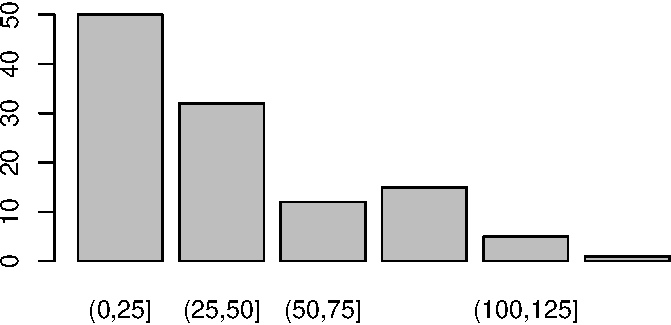
\includegraphics[keepaspectratio]{Lecture-8-Exploratory-Data-Analysis_files/figure-pdf/unnamed-chunk-16-1.pdf}}

\begin{watch}{}{}
    \href{https://youtu.be/SqOE-rSd-_U}{Creating Basic Visualizations}
\end{watch}

Exploratory Data Analysis, and in particular these 6 steps, is something
we should carry out every time we start working with new datasets. We do
not want to jump into analyzing a dataset without knowing what it looks
like or if changes need to be made. After a while, these steps will
become second nature to us and we will be able to carry them out
relatively quickly.

\bookmarksetup{startatroot}

\chapter{Loading Data in R \& EDA}\label{loading-data-in-r-eda}

\section{Loading Data into R}\label{loading-data-into-r}

Sometimes we are interested in using data that isn't in R. If this is
the case, we will have to load the data into R ourselves using a CSV
file. To follow along with this lecture writeup, you should download the
dataset called ``Data\_200\_df.csv'' on Canvas under the Modules. Now to
load data into R there are several different ways we can do it. One way
is using the \emph{read.csv()} function where we pass the file path into
the function.

\begin{Shaded}
\begin{Highlighting}[]
\CommentTok{\# My file is saved on my Desktop, yours might be saved under Downloads}
\NormalTok{Data\_200\_df }\OtherTok{\textless{}{-}} \FunctionTok{read.csv}\NormalTok{(}\StringTok{"Desktop/Data\_200\_df.csv"}\NormalTok{)}
\end{Highlighting}
\end{Shaded}

An easier method to load data into R (so we don't have to memorize the
function!) is to go to ``File -\(>\) Import Dataset -\(>\) From Text
(base)'' and then select the file we want to import. Using this method
also makes it easier for us to customize our request like identifying if
we have row/column headers or if all of the strings should be factors.

\begin{watch}{}{}
    \href{https://youtu.be/603gU61EWQ4}{Loading Data into R}
\end{watch}

\section{Converting character vectors to
factors}\label{converting-character-vectors-to-factors}

Now that we have the data loaded into our R environment, we can start to
do some Exploratory Data Analysis (EDA) on it. The first thing we will
want to do is look at the structure of the dataset to see what we are
dealing with. This can be done using the \emph{str()} function. In our
case here, we do not have any documentation to compare our data or to
learn about the dataset.

\begin{Shaded}
\begin{Highlighting}[]
\FunctionTok{str}\NormalTok{(Data\_200\_df)}
\end{Highlighting}
\end{Shaded}

\begin{verbatim}
'data.frame':   50 obs. of  6 variables:
 $ names : chr  "Theresa" "Clyde" "Katrina" "Ricky" ...
 $ ages  : int  21 20 19 19 19 23 18 21 24 23 ...
 $ state : chr  "NY" "NC" "NY" "NY" ...
 $ year  : chr  "Freshman" "Freshman" "Sophmore" "Sophmore" ...
 $ majors: chr  "Psych" "Comp-Sci" "Math" "Psych" ...
 $ sport : int  0 1 1 0 1 1 0 0 0 0 ...
\end{verbatim}

Looking at this, it would probably make sense to turn a couple of these
columns into factors instead of having them be character/integer
vectors. This can be done using the \emph{factor()} function and then
altering the levels if need be (since sport is given as 0 or 1 we may
want to alter the level name to No and Yes). We should only convert a
vector to a factor column if there are finite number of categories and
there are multiple occurrences of each category. So, we will not need to
convert the ``names'' column since they are all unique and there are
virtually infinite number of possibilities.

\begin{Shaded}
\begin{Highlighting}[]
\NormalTok{Data\_200\_df}\SpecialCharTok{$}\NormalTok{state\_f }\OtherTok{\textless{}{-}} \FunctionTok{factor}\NormalTok{(Data\_200\_df}\SpecialCharTok{$}\NormalTok{state)}
\NormalTok{Data\_200\_df}\SpecialCharTok{$}\NormalTok{year\_f }\OtherTok{\textless{}{-}} \FunctionTok{factor}\NormalTok{(Data\_200\_df}\SpecialCharTok{$}\NormalTok{year)}
\NormalTok{Data\_200\_df}\SpecialCharTok{$}\NormalTok{majors\_f }\OtherTok{\textless{}{-}} \FunctionTok{factor}\NormalTok{(Data\_200\_df}\SpecialCharTok{$}\NormalTok{majors)}

\NormalTok{Data\_200\_df}\SpecialCharTok{$}\NormalTok{sport\_f }\OtherTok{\textless{}{-}} \FunctionTok{as.factor}\NormalTok{(Data\_200\_df}\SpecialCharTok{$}\NormalTok{sport)}
\FunctionTok{levels}\NormalTok{(Data\_200\_df}\SpecialCharTok{$}\NormalTok{sport\_f) }\OtherTok{\textless{}{-}} \FunctionTok{c}\NormalTok{(}\StringTok{"No"}\NormalTok{, }\StringTok{"Yes"}\NormalTok{)}
\end{Highlighting}
\end{Shaded}

\begin{watch}{}{}
    \href{https://youtu.be/4oSEQDN8C1c}{Converting Vectors into Factors}
\end{watch}

\section{Utilizing the Table
function}\label{utilizing-the-table-function}

To better understand the dataset, it is helpful to calculate some
descriptive statistics and create some visualizations as well. To
calculate descriptive statistics for a categorical variable we can use
the \emph{table()} function. This will tell us how many times each
category occurs.

\begin{Shaded}
\begin{Highlighting}[]
\FunctionTok{table}\NormalTok{(Data\_200\_df}\SpecialCharTok{$}\NormalTok{year)}
\end{Highlighting}
\end{Shaded}

\begin{verbatim}

Freshman   Junior   Senior Sophmore 
      15       12       10       13 
\end{verbatim}

\begin{Shaded}
\begin{Highlighting}[]
\FunctionTok{barplot}\NormalTok{(}\FunctionTok{table}\NormalTok{(Data\_200\_df}\SpecialCharTok{$}\NormalTok{year))}
\end{Highlighting}
\end{Shaded}

\pandocbounded{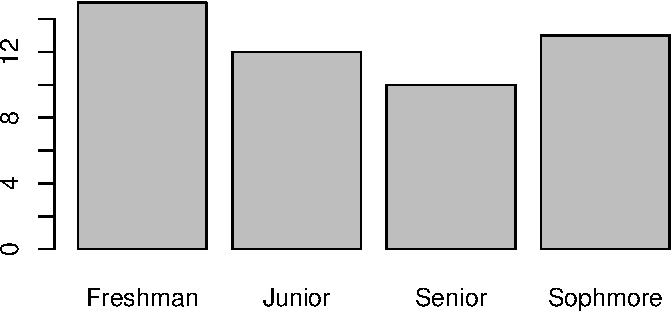
\includegraphics[keepaspectratio]{Lecture-9-More-EDA-and-Loading-in-Data_files/figure-pdf/unnamed-chunk-5-1.pdf}}

\begin{Shaded}
\begin{Highlighting}[]
\FunctionTok{table}\NormalTok{(Data\_200\_df}\SpecialCharTok{$}\NormalTok{majors)}
\end{Highlighting}
\end{Shaded}

\begin{verbatim}

    Chem Comp-Sci     Data  History     Math    Psych 
      12        9       10        2       10        7 
\end{verbatim}

\begin{Shaded}
\begin{Highlighting}[]
\FunctionTok{barplot}\NormalTok{(}\FunctionTok{table}\NormalTok{(Data\_200\_df}\SpecialCharTok{$}\NormalTok{majors))}
\end{Highlighting}
\end{Shaded}

\pandocbounded{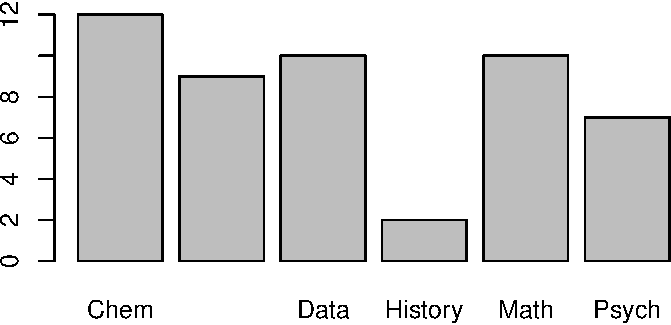
\includegraphics[keepaspectratio]{Lecture-9-More-EDA-and-Loading-in-Data_files/figure-pdf/unnamed-chunk-6-1.pdf}}

So, this shows us the number of students who are Juniors, and the number
of students who are Data majors, but can we determine how many Junior
Data majors we have? One way we could do this is by using a logical
vector:

\begin{Shaded}
\begin{Highlighting}[]
\FunctionTok{sum}\NormalTok{(Data\_200\_df}\SpecialCharTok{$}\NormalTok{year}\SpecialCharTok{==}\StringTok{"Junior"} \SpecialCharTok{\&}\NormalTok{ Data\_200\_df}\SpecialCharTok{$}\NormalTok{majors}\SpecialCharTok{==}\StringTok{"Data"}\NormalTok{)}
\end{Highlighting}
\end{Shaded}

\begin{verbatim}
[1] 2
\end{verbatim}

If we are interested in other combinations we certainly could carry out
the process again and again for all 24 combinations. Another way that
will count the number of students who fall into each category is to use
the \emph{table()} function but pass two categorical variables into it.
It will count the number of occurrences for each combination of
groupings.

\begin{Shaded}
\begin{Highlighting}[]
\FunctionTok{table}\NormalTok{(Data\_200\_df}\SpecialCharTok{$}\NormalTok{majors, Data\_200\_df}\SpecialCharTok{$}\NormalTok{year)}
\end{Highlighting}
\end{Shaded}

\begin{verbatim}
          
           Freshman Junior Senior Sophmore
  Chem            4      3      2        3
  Comp-Sci        4      3      1        1
  Data            1      2      2        5
  History         1      1      0        0
  Math            3      1      4        2
  Psych           2      2      1        2
\end{verbatim}

\begin{watch}{}{}
    \href{https://youtu.be/Oq4GZnTAHNk}{Using the \textit{table()} Function with multiple variables}
\end{watch}

\section{Utilizing the Aggregate
function}\label{utilizing-the-aggregate-function}

Another type of descriptive statistic that we can calculate is the mean
on one of the variables (age in our case). While this is helpful, it
might also be interesting to see the mean age by major, and to do this
we can use a logical vector within our index-selection brackets.

\begin{Shaded}
\begin{Highlighting}[]
\FunctionTok{mean}\NormalTok{(Data\_200\_df}\SpecialCharTok{$}\NormalTok{ages)}
\end{Highlighting}
\end{Shaded}

\begin{verbatim}
[1] 20.7
\end{verbatim}

\begin{Shaded}
\begin{Highlighting}[]
\FunctionTok{mean}\NormalTok{(Data\_200\_df}\SpecialCharTok{$}\NormalTok{ages[Data\_200\_df}\SpecialCharTok{$}\NormalTok{majors}\SpecialCharTok{==}\StringTok{"Psych"}\NormalTok{])}
\end{Highlighting}
\end{Shaded}

\begin{verbatim}
[1] 20.42857
\end{verbatim}

\begin{Shaded}
\begin{Highlighting}[]
\FunctionTok{mean}\NormalTok{(Data\_200\_df}\SpecialCharTok{$}\NormalTok{ages[Data\_200\_df}\SpecialCharTok{$}\NormalTok{majors}\SpecialCharTok{==}\StringTok{"Chem"}\NormalTok{])}
\end{Highlighting}
\end{Shaded}

\begin{verbatim}
[1] 20.91667
\end{verbatim}

\begin{Shaded}
\begin{Highlighting}[]
\FunctionTok{mean}\NormalTok{(Data\_200\_df}\SpecialCharTok{$}\NormalTok{ages[Data\_200\_df}\SpecialCharTok{$}\NormalTok{majors}\SpecialCharTok{==}\StringTok{"History"}\NormalTok{])}
\end{Highlighting}
\end{Shaded}

\begin{verbatim}
[1] 18
\end{verbatim}

Running a line of code for every major is tedious and cumbersome. To do
it more efficiently we could use the \emph{aggregate()} function. In
this function, we will pass in the variable we want to calculate, then
specify what we want to group \emph{by} (which needs to be in the
\emph{list()} function and be a categorical variable), and finally
specifying the function we want to run. The general setup for this
function will be:

\begin{verbatim}
aggregate(Quantitative_Variable, by = list(Categorical_Grouping_Variable), math_function)
\end{verbatim}

An example of this function can be seen below:

\begin{Shaded}
\begin{Highlighting}[]
\FunctionTok{aggregate}\NormalTok{(Data\_200\_df}\SpecialCharTok{$}\NormalTok{ages, }\AttributeTok{by=}\FunctionTok{list}\NormalTok{(Data\_200\_df}\SpecialCharTok{$}\NormalTok{majors), mean)}
\end{Highlighting}
\end{Shaded}

\begin{verbatim}
   Group.1        x
1     Chem 20.91667
2 Comp-Sci 21.44444
3     Data 19.90000
4  History 18.00000
5     Math 21.30000
6    Psych 20.42857
\end{verbatim}

\begin{watch}{}{}
    \href{https://youtu.be/k5Wgr1VVUhw}{Using the \textit{aggregate()} Function}
\end{watch}

The way we can read the output from above is that the average age of
Chemistry majors is 20.92, the average age of Computer Science majors is
21.44, and so on. We can divide our population up into more groups if we
want. For instance, maybe we want to find the average age of people
based on their major and whether they play a sport. To do this we will
pass in two variables in the \emph{by} argument.

\begin{Shaded}
\begin{Highlighting}[]
\FunctionTok{aggregate}\NormalTok{(Data\_200\_df}\SpecialCharTok{$}\NormalTok{ages, }
          \AttributeTok{by=}\FunctionTok{list}\NormalTok{(}\AttributeTok{majors =}\NormalTok{ Data\_200\_df}\SpecialCharTok{$}\NormalTok{majors, }
                  \AttributeTok{sports =}\NormalTok{ Data\_200\_df}\SpecialCharTok{$}\NormalTok{sport), }
\NormalTok{          mean)}
\end{Highlighting}
\end{Shaded}

\begin{verbatim}
     majors sports        x
1      Chem      0 20.60000
2  Comp-Sci      0 21.80000
3      Data      0 20.60000
4      Math      0 21.20000
5     Psych      0 21.00000
6      Chem      1 21.14286
7  Comp-Sci      1 21.00000
8      Data      1 19.20000
9   History      1 18.00000
10     Math      1 21.40000
11    Psych      1 19.00000
\end{verbatim}

For this output, we would interpret it similarly. We would say the
average age of Chemistry majors who do not play a sport is 20.60, and
the average age of Chemistry majors who play a sport is 21.14. We can
then do it for all possible combinations of majors and whether they play
a sport or not. We can also carry this out using different functions
like sd, length, median, and so on.

\begin{Shaded}
\begin{Highlighting}[]
\FunctionTok{aggregate}\NormalTok{(Data\_200\_df}\SpecialCharTok{$}\NormalTok{age, }\AttributeTok{by=}\FunctionTok{list}\NormalTok{(}\AttributeTok{state=}\NormalTok{ Data\_200\_df}\SpecialCharTok{$}\NormalTok{state), sd)}
\end{Highlighting}
\end{Shaded}

\begin{verbatim}
  state        x
1    MD 2.345208
2    NC 1.378405
3    NY 2.101805
4    PA 2.645751
5    VA 1.612452
6    WV 2.438123
\end{verbatim}

\begin{watch}{}{}
    \href{https://youtu.be/OsadIjZEIR0}{Using the \textit{aggregate()} Function with Multiple Groupings}
\end{watch}

Within this section, we have learned two powerful functions which help
us summarize categorical and quantitative data. We should think about
what data we have present though before we run the code. If we try to
run the table function on data that is not categorical (with relatively
few categories) or if we try to use the aggregate function and group by
quantitative data then the output will not be readable due to the number
of possibilities. Therefore, it is important to think about what type of
data we are passing into each function and whether the output is
particularly useful.

\bookmarksetup{startatroot}

\chapter{Probability Distributions}\label{probability-distributions}

When it comes to data, it normally follows some pattern. The trouble is
trying to identify what the pattern is. There are a few ways we could do
this; one way is to try and guess the pattern using specific examples or
we could observe large amounts of data to try and find a pattern. The
first method will require us to learn about different probability
distributions and their properties while the second method will require
simulating datasets and looking at the results.

\section{Overview of Probability}\label{overview-of-probability}

To understand probability distributions, we should probably have a brief
review of the topic. Probability is the measure of the likelihood that
an event will occur. This likelihood is expressed as a number between 0
and 1, where 0 will indicate impossibility and 1 indicate certainty. The
value will always be between 0 and 1 with the sum of probabilities being
equal to 1. Some short-hand which you might seen is \emph{P(A)}, which
indicates the ``probability of event A occurring''.

\begin{watch}{}{}
    \href{https://youtu.be/BxHJLWyJWZo}{Probability Overview}
\end{watch}

\section{Discrete Probability}\label{discrete-probability}

\subsection{Bernoulli Distribution}\label{bernoulli-distribution}

If we think about flipping a coin, we might ask what the probability of
landing on heads or tails is. We know that there is an equal chance (as
long as the coin is fair) of landing on either side, so we will say
\(P(H)=0.5\) and \(P(T)=0.5\). But, if we flip the coin two times we
will not always get heads and tails 50\% of the time (that is 1 head and
1 tail). To see this phenomenon we can carry out a simulation in R.

\begin{Shaded}
\begin{Highlighting}[]
\FunctionTok{sample}\NormalTok{(}\FunctionTok{c}\NormalTok{(}\StringTok{"Head"}\NormalTok{, }\StringTok{"Tail"}\NormalTok{), }\DecValTok{2}\NormalTok{, }\AttributeTok{replace=}\ConstantTok{TRUE}\NormalTok{)}
\end{Highlighting}
\end{Shaded}

\begin{verbatim}
[1] "Tail" "Tail"
\end{verbatim}

\begin{Shaded}
\begin{Highlighting}[]
\FunctionTok{sample}\NormalTok{(}\FunctionTok{c}\NormalTok{(}\StringTok{"Head"}\NormalTok{, }\StringTok{"Tail"}\NormalTok{), }\DecValTok{2}\NormalTok{, }\AttributeTok{replace=}\ConstantTok{TRUE}\NormalTok{)}
\end{Highlighting}
\end{Shaded}

\begin{verbatim}
[1] "Head" "Tail"
\end{verbatim}

\begin{Shaded}
\begin{Highlighting}[]
\FunctionTok{sample}\NormalTok{(}\FunctionTok{c}\NormalTok{(}\StringTok{"Head"}\NormalTok{, }\StringTok{"Tail"}\NormalTok{), }\DecValTok{2}\NormalTok{, }\AttributeTok{replace=}\ConstantTok{TRUE}\NormalTok{)}
\end{Highlighting}
\end{Shaded}

\begin{verbatim}
[1] "Tail" "Head"
\end{verbatim}

We can take this a step further by flipping 10 coins. We would expect to
see roughly 5 Heads and 5 Tails, but we would not expect to always see 5
heads and 5 tails. As we can see from the simulation below, we sometimes
get only 3 or 4 Heads and the rest Tails. The more observations we have
(that is the more coin flips we do) the closer we should be to the
expected proportion (50-50). A simulation below produced heads in 30\%
of the coin flips, but if we flip 10,000 coins we would find it highly
unusual to witness heads only 30\% of the time, as we expect the
proportion of heads to be much closer to 50\%.

\begin{Shaded}
\begin{Highlighting}[]
\FunctionTok{sample}\NormalTok{(}\FunctionTok{c}\NormalTok{(}\StringTok{"H"}\NormalTok{, }\StringTok{"T"}\NormalTok{), }\DecValTok{10}\NormalTok{, }\AttributeTok{replace=}\ConstantTok{TRUE}\NormalTok{)}
\end{Highlighting}
\end{Shaded}

\begin{verbatim}
 [1] "H" "H" "H" "T" "T" "H" "T" "H" "H" "T"
\end{verbatim}

\begin{Shaded}
\begin{Highlighting}[]
\FunctionTok{sample}\NormalTok{(}\FunctionTok{c}\NormalTok{(}\StringTok{"H"}\NormalTok{, }\StringTok{"T"}\NormalTok{), }\DecValTok{10}\NormalTok{, }\AttributeTok{replace=}\ConstantTok{TRUE}\NormalTok{)}
\end{Highlighting}
\end{Shaded}

\begin{verbatim}
 [1] "H" "H" "H" "T" "H" "T" "H" "H" "H" "H"
\end{verbatim}

\begin{Shaded}
\begin{Highlighting}[]
\FunctionTok{sample}\NormalTok{(}\FunctionTok{c}\NormalTok{(}\StringTok{"H"}\NormalTok{, }\StringTok{"T"}\NormalTok{), }\DecValTok{10}\NormalTok{, }\AttributeTok{replace=}\ConstantTok{TRUE}\NormalTok{)}
\end{Highlighting}
\end{Shaded}

\begin{verbatim}
 [1] "H" "T" "H" "T" "T" "T" "T" "H" "H" "H"
\end{verbatim}

\begin{Shaded}
\begin{Highlighting}[]
\NormalTok{flip }\OtherTok{\textless{}{-}} \FunctionTok{sample}\NormalTok{(}\FunctionTok{c}\NormalTok{(}\StringTok{"H"}\NormalTok{, }\StringTok{"T"}\NormalTok{), }\DecValTok{10000}\NormalTok{, }\AttributeTok{replace=}\ConstantTok{TRUE}\NormalTok{)}
\FunctionTok{table}\NormalTok{(flip)}
\end{Highlighting}
\end{Shaded}

\begin{verbatim}
flip
   H    T 
4998 5002 
\end{verbatim}

\begin{Shaded}
\begin{Highlighting}[]
\FunctionTok{barplot}\NormalTok{(}\FunctionTok{table}\NormalTok{(flip))}
\end{Highlighting}
\end{Shaded}

\pandocbounded{\includegraphics[keepaspectratio]{Lecture-10-Probability-Distributions_files/figure-pdf/unnamed-chunk-4-1.pdf}}

What would happen though if the coin wasn't fair and gave us
\(P(H)=0.75\)? Then we would expect to get Heads roughly 75\% of the
time and Tails roughly 25\% of the time. To do this simulation in R, we
could alter the probabilities of each value in the vector using the
\emph{prob} argument.

\begin{Shaded}
\begin{Highlighting}[]
\NormalTok{unfair }\OtherTok{\textless{}{-}} \FunctionTok{sample}\NormalTok{(}\FunctionTok{c}\NormalTok{(}\StringTok{"H"}\NormalTok{, }\StringTok{"T"}\NormalTok{), }\DecValTok{10000}\NormalTok{, }\AttributeTok{prob=}\FunctionTok{c}\NormalTok{(.}\DecValTok{75}\NormalTok{,.}\DecValTok{25}\NormalTok{), }\AttributeTok{replace=}\ConstantTok{TRUE}\NormalTok{)}
\FunctionTok{table}\NormalTok{(unfair)}
\end{Highlighting}
\end{Shaded}

\begin{verbatim}
unfair
   H    T 
7401 2599 
\end{verbatim}

\begin{Shaded}
\begin{Highlighting}[]
\FunctionTok{barplot}\NormalTok{(}\FunctionTok{table}\NormalTok{(unfair))}
\end{Highlighting}
\end{Shaded}

\pandocbounded{\includegraphics[keepaspectratio]{Lecture-10-Probability-Distributions_files/figure-pdf/unnamed-chunk-5-1.pdf}}

The examples we have seen will lead us to the idea of the
\textbf{Bernoulli Distribution}. For this probability distribution, the
results are either Success (1) or Failure (0). The probability of
success is usually denoted by \(p\) with the probability of failure
being \(q=1-p\). The probability distribution function can be written
as: \[ P(X=k) = p^k (1-p)^{1-k}\]

where \(k=1\) means success and \(k=0\) means failure. Other things to
note about this distribution are that the mean will be \(\mu=p\) (note:
\(\mu\) represents the population mean and is pronounced ``mew'') and
the standard deviation will be \(\sigma= \sqrt{p(1-p)}\). (note:
\(\sigma\) represents the population standard deviation is the
pronounced ``sigma'').

\subsection{Utilizing the Matrix and Apply
function}\label{utilizing-the-matrix-and-apply-function}

The Bernoulli distribution will only concern itself with a single
outcome, but what if we are instead interested in flipping a coin 10
times and counting the number of heads that occur? We have already seen
that we would expect roughly 5 heads, but it will not always be exact.
To model this problem, we could do some simulations in R again. For this
problem, I will instead use 1 (to represent Heads) and 0 (to represent
Tails) as well as using the \emph{matrix()} function and \emph{apply()}
function.

The \emph{matrix()} function will allow us to fill in a matrix with
values from our sample. We will indicate the number of rows we want in
the matrix and it will figure out how many columns are needed to
accommodate all of the data we give it. We should be aware though that
it will start repeating the data if we do not pass it enough data to
complete the rectangular matrix. In the example below, we can see how it
will fill in the matrix if we pass it 10 values and indicate we only
want 3 rows:

\begin{Shaded}
\begin{Highlighting}[]
\FunctionTok{matrix}\NormalTok{(}\DecValTok{1}\SpecialCharTok{:}\DecValTok{10}\NormalTok{, }\AttributeTok{nrow=}\DecValTok{3}\NormalTok{)}
\end{Highlighting}
\end{Shaded}

\begin{verbatim}
Warning in matrix(1:10, nrow = 3): data length [10] is not a sub-multiple or
multiple of the number of rows [3]
\end{verbatim}

\begin{verbatim}
     [,1] [,2] [,3] [,4]
[1,]    1    4    7   10
[2,]    2    5    8    1
[3,]    3    6    9    2
\end{verbatim}

The \emph{apply()} function will allow us to apply a function on a
matrix in R. To use this function, we will need to pass it a matrix and
indicate if we want to do the function across the rows (MARGIN=1) or the
columns (MARGIN=2). Finally, we do have to pass it a function to carry
out (like mean, sum, sd, etc.).

\begin{Shaded}
\begin{Highlighting}[]
\NormalTok{x\_mat }\OtherTok{\textless{}{-}} \FunctionTok{matrix}\NormalTok{(}\DecValTok{1}\SpecialCharTok{:}\DecValTok{10}\NormalTok{, }\AttributeTok{nrow=}\DecValTok{3}\NormalTok{)}
\end{Highlighting}
\end{Shaded}

\begin{verbatim}
Warning in matrix(1:10, nrow = 3): data length [10] is not a sub-multiple or
multiple of the number of rows [3]
\end{verbatim}

\begin{Shaded}
\begin{Highlighting}[]
\FunctionTok{apply}\NormalTok{(x\_mat, }\AttributeTok{MARGIN=}\DecValTok{1}\NormalTok{, sum) }\CommentTok{\# Calculating the sum for each row}
\end{Highlighting}
\end{Shaded}

\begin{verbatim}
[1] 22 16 20
\end{verbatim}

\begin{Shaded}
\begin{Highlighting}[]
\FunctionTok{apply}\NormalTok{(x\_mat, }\AttributeTok{MARGIN=}\DecValTok{2}\NormalTok{, sum) }\CommentTok{\# Calculating the sum for each column}
\end{Highlighting}
\end{Shaded}

\begin{verbatim}
[1]  6 15 24 13
\end{verbatim}

I encourage you to play around with the \emph{matrix()} and
\emph{apply()} functions to get a sense of how they work since we will
be using them to do simulations in R quite a bit.

\begin{watch}{}{}
    \href{https://youtu.be/pc5_0-_KRuo}{Using the \textit{matrix()} and \textit{apply()} Functions}
\end{watch}

\subsection{Binomial Distribution}\label{binomial-distribution}

In the simulation below, we are flipping 10 coins (columns), writing
down the results, and repeating this process a total of 12 times (rows).
We then count the number of heads that occur in each row. Visualizing it
as a table allows us to see the number of times each result occurred. We
can see that we occasionally got 7 Heads, but the majority of the time
we had close to 5 Heads.

\begin{Shaded}
\begin{Highlighting}[]
\NormalTok{flips }\OtherTok{\textless{}{-}} \FunctionTok{matrix}\NormalTok{(}\FunctionTok{sample}\NormalTok{(}\FunctionTok{c}\NormalTok{(}\DecValTok{1}\NormalTok{, }\DecValTok{0}\NormalTok{), }\DecValTok{10}\SpecialCharTok{*}\DecValTok{12}\NormalTok{, }\AttributeTok{replace=}\ConstantTok{TRUE}\NormalTok{), }\AttributeTok{nrow=}\DecValTok{12}\NormalTok{)}
\NormalTok{flips}
\end{Highlighting}
\end{Shaded}

\begin{verbatim}
      [,1] [,2] [,3] [,4] [,5] [,6] [,7] [,8] [,9] [,10]
 [1,]    0    1    1    1    1    0    1    1    0     0
 [2,]    1    1    0    1    1    1    0    1    0     1
 [3,]    1    1    1    1    1    1    0    1    0     0
 [4,]    1    1    0    1    0    1    1    1    0     0
 [5,]    1    1    1    1    0    1    0    0    0     0
 [6,]    1    1    1    0    0    1    1    1    0     0
 [7,]    0    1    0    1    1    0    0    1    0     1
 [8,]    1    0    1    0    0    0    0    1    0     1
 [9,]    0    1    1    1    1    1    1    0    0     0
[10,]    1    0    0    1    1    1    0    0    1     0
[11,]    0    1    1    0    0    1    0    0    1     0
[12,]    1    0    1    0    0    1    1    0    0     0
\end{verbatim}

\begin{Shaded}
\begin{Highlighting}[]
\NormalTok{nheads }\OtherTok{\textless{}{-}} \FunctionTok{apply}\NormalTok{(flips, }\AttributeTok{MARGIN=}\DecValTok{1}\NormalTok{, }\AttributeTok{FUN=}\NormalTok{sum)}
\NormalTok{nheads}
\end{Highlighting}
\end{Shaded}

\begin{verbatim}
 [1] 6 7 7 6 5 6 5 4 6 5 4 4
\end{verbatim}

\begin{Shaded}
\begin{Highlighting}[]
\FunctionTok{table}\NormalTok{(nheads) }\CommentTok{\# Results of flipping 10 coins 12 times}
\end{Highlighting}
\end{Shaded}

\begin{verbatim}
nheads
4 5 6 7 
3 3 4 2 
\end{verbatim}

\begin{Shaded}
\begin{Highlighting}[]
\FunctionTok{barplot}\NormalTok{(}\FunctionTok{table}\NormalTok{(}\FunctionTok{factor}\NormalTok{(nheads, }\AttributeTok{levels=}\DecValTok{0}\SpecialCharTok{:}\DecValTok{10}\NormalTok{)))}
\end{Highlighting}
\end{Shaded}

\pandocbounded{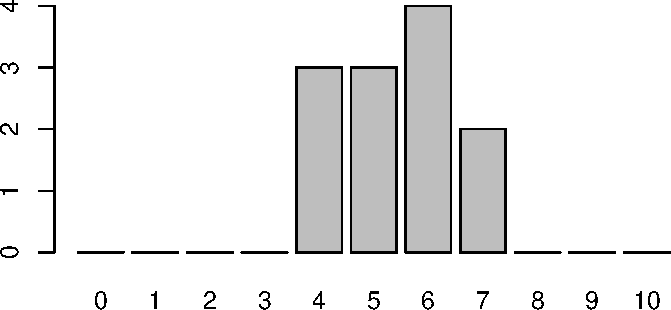
\includegraphics[keepaspectratio]{Lecture-10-Probability-Distributions_files/figure-pdf/unnamed-chunk-8-1.pdf}}

Instead of just doing it 12 times, what if we did it 100 times or even
10,000 times? How might our counts and barplot look?

\begin{Shaded}
\begin{Highlighting}[]
\NormalTok{number\_of\_times }\OtherTok{\textless{}{-}} \DecValTok{100}
\NormalTok{flips }\OtherTok{\textless{}{-}} \FunctionTok{matrix}\NormalTok{(}\FunctionTok{sample}\NormalTok{(}\FunctionTok{c}\NormalTok{(}\DecValTok{1}\NormalTok{, }\DecValTok{0}\NormalTok{), }\DecValTok{10}\SpecialCharTok{*}\NormalTok{number\_of\_times, }\AttributeTok{replace=}\ConstantTok{TRUE}\NormalTok{), }\AttributeTok{nrow=}\NormalTok{number\_of\_times)}
\NormalTok{nheads }\OtherTok{\textless{}{-}} \FunctionTok{apply}\NormalTok{(flips, }\AttributeTok{MARGIN=}\DecValTok{1}\NormalTok{, }\AttributeTok{FUN=}\NormalTok{sum)}
\FunctionTok{table}\NormalTok{(nheads) }\CommentTok{\# Results of flipping 10 coins 100 times}
\end{Highlighting}
\end{Shaded}

\begin{verbatim}
nheads
 1  2  3  4  5  6  7  8  9 
 1  8 12 16 28 19 10  4  2 
\end{verbatim}

\begin{Shaded}
\begin{Highlighting}[]
\FunctionTok{barplot}\NormalTok{(}\FunctionTok{table}\NormalTok{(}\FunctionTok{factor}\NormalTok{(nheads, }\AttributeTok{levels=}\DecValTok{0}\SpecialCharTok{:}\DecValTok{10}\NormalTok{)))}
\end{Highlighting}
\end{Shaded}

\pandocbounded{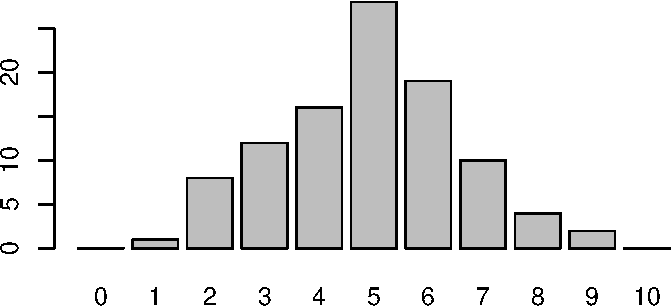
\includegraphics[keepaspectratio]{Lecture-10-Probability-Distributions_files/figure-pdf/unnamed-chunk-9-1.pdf}}

\begin{Shaded}
\begin{Highlighting}[]
\NormalTok{number\_of\_times }\OtherTok{\textless{}{-}} \DecValTok{10000}
\NormalTok{flips }\OtherTok{\textless{}{-}} \FunctionTok{matrix}\NormalTok{(}\FunctionTok{sample}\NormalTok{(}\FunctionTok{c}\NormalTok{(}\DecValTok{1}\NormalTok{, }\DecValTok{0}\NormalTok{), }\DecValTok{10}\SpecialCharTok{*}\NormalTok{number\_of\_times, }\AttributeTok{replace=}\ConstantTok{TRUE}\NormalTok{), }\AttributeTok{nrow=}\NormalTok{number\_of\_times)}
\NormalTok{nheads }\OtherTok{\textless{}{-}} \FunctionTok{apply}\NormalTok{(flips, }\AttributeTok{MARGIN=}\DecValTok{1}\NormalTok{, }\AttributeTok{FUN=}\NormalTok{sum)}
\FunctionTok{table}\NormalTok{(nheads) }\CommentTok{\# Results of flipping 10 coins 100 times}
\end{Highlighting}
\end{Shaded}

\begin{verbatim}
nheads
   0    1    2    3    4    5    6    7    8    9   10 
  15   90  404 1186 2068 2458 2036 1184  440  106   13 
\end{verbatim}

\begin{Shaded}
\begin{Highlighting}[]
\FunctionTok{barplot}\NormalTok{(}\FunctionTok{table}\NormalTok{(}\FunctionTok{factor}\NormalTok{(nheads, }\AttributeTok{levels=}\DecValTok{0}\SpecialCharTok{:}\DecValTok{10}\NormalTok{)))}
\end{Highlighting}
\end{Shaded}

\pandocbounded{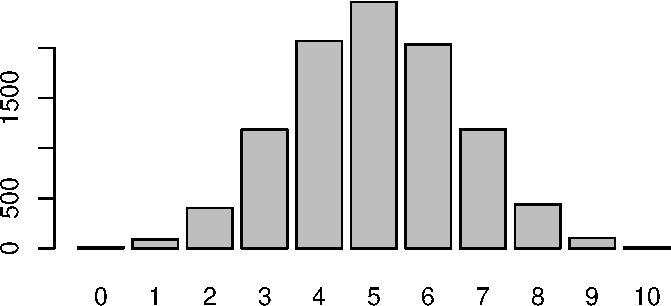
\includegraphics[keepaspectratio]{Lecture-10-Probability-Distributions_files/figure-pdf/unnamed-chunk-10-1.pdf}}

In the simulations, the individual flips are represented by the
Bernoulli distribution (success or failure). The sequence of flipping to
coin 10 times is known as a Bernoulli trial. The \textbf{Binomial
Distribution} represents the number of successes in \(n\) Bernoulli
trials. Notice that when \(n=1\) we have a Bernoulli Distribution. The
probability distribution function can be written as:

\[ \text{P(X=k)}={n\choose k}p^k(1-p)^{n-k}=\frac{n!}{(n-k)!k!}p^kq^{n-k}\]

where \(n\) is the number of trials, \(k\) is the number of successes,
and \(p\) is the probability of success. Other things to note about this
distribution are that the mean will be \(\mu=np\) and the standard
deviation will be \(\sigma=\sqrt{np(1-p)}\).

\begin{watch}{}{}
    \href{https://youtu.be/RObY6UvS6fs}{Simulating a Binomial Distribution}
\end{watch}

\subsection{Theoretical vs Empirical
Probability}\label{theoretical-vs-empirical-probability}

Now that we know a few different probability distribution functions, we
should probably discuss the 2 main ways we can calculate probabilities.
The first way is to calculate it \textbf{theoretically} if we know the
underlying distribution. To do this, we would need to evaluate the
probability distribution function at the desired value. If we do not,
then we can calculate it \textbf{empirically} if we have a large number
of observations available to us. To do this, we will simply see the
proportion of values that meet the desired criteria.

Take the following example: If we were to flip a coin 10 times, what is
the probability that we would end up with exactly 4 heads? This is a
Binomial Distribution with \(n=10\) and \(p=0.5\), which is can be
written as Bin(10,0.5), so:

\[ \text{P(X=4)}={10\choose 4}0.5^4(1-0.5)^{10-4}\approx 0.2050781 \]

\begin{Shaded}
\begin{Highlighting}[]
\FunctionTok{choose}\NormalTok{(}\DecValTok{10}\NormalTok{,}\DecValTok{4}\NormalTok{)}\SpecialCharTok{*}\FloatTok{0.5}\SpecialCharTok{\^{}}\DecValTok{4}\SpecialCharTok{*}\NormalTok{(}\DecValTok{1}\FloatTok{{-}0.5}\NormalTok{)}\SpecialCharTok{\^{}}\NormalTok{(}\DecValTok{10{-}4}\NormalTok{)}
\end{Highlighting}
\end{Shaded}

\begin{verbatim}
[1] 0.2050781
\end{verbatim}

\begin{Shaded}
\begin{Highlighting}[]
\FunctionTok{factorial}\NormalTok{(}\DecValTok{10}\NormalTok{)}\SpecialCharTok{/}\NormalTok{(}\FunctionTok{factorial}\NormalTok{(}\DecValTok{6}\NormalTok{)}\SpecialCharTok{*}\FunctionTok{factorial}\NormalTok{(}\DecValTok{4}\NormalTok{))}\SpecialCharTok{*}\FloatTok{0.5}\SpecialCharTok{\^{}}\DecValTok{4}\SpecialCharTok{*}\FloatTok{0.5}\SpecialCharTok{\^{}}\DecValTok{6}
\end{Highlighting}
\end{Shaded}

\begin{verbatim}
[1] 0.2050781
\end{verbatim}

This is called the Theoretical Probability since we know what the
distribution is for our question. If we did not know what the
probability distribution was then we can always simulate it similarly to
what we did above. For this, we simulated 10,000 10-flip trials and
counted the number of heads in each trial:

\begin{Shaded}
\begin{Highlighting}[]
\FunctionTok{table}\NormalTok{(nheads)}
\end{Highlighting}
\end{Shaded}

\begin{verbatim}
nheads
   0    1    2    3    4    5    6    7    8    9   10 
  15   90  404 1186 2068 2458 2036 1184  440  106   13 
\end{verbatim}

\begin{Shaded}
\begin{Highlighting}[]
\DecValTok{2068}\SpecialCharTok{/}\DecValTok{10000}
\end{Highlighting}
\end{Shaded}

\begin{verbatim}
[1] 0.2068
\end{verbatim}

This is called the Empirical Probability since we have a large number of
observations. We can see that the proportion of 4 heads is roughly
0.2068 when we ran it 10,000 times. Notice this is very close to our
theoretical probability! We can do something similar if our coin is not
fair. For instance, if we flip 10 coins 10,000 times when the
probability of heads was 0.75 then we might get results that look like
this:

\begin{Shaded}
\begin{Highlighting}[]
\NormalTok{n }\OtherTok{\textless{}{-}} \DecValTok{10000} \CommentTok{\# number of times flipping the 10 coins}
\NormalTok{flips }\OtherTok{\textless{}{-}} \FunctionTok{matrix}\NormalTok{(}\FunctionTok{sample}\NormalTok{(}\FunctionTok{c}\NormalTok{(}\DecValTok{1}\NormalTok{, }\DecValTok{0}\NormalTok{), }\DecValTok{10}\SpecialCharTok{*}\NormalTok{n, }\AttributeTok{replace=}\ConstantTok{TRUE}\NormalTok{, }\AttributeTok{prob=}\FunctionTok{c}\NormalTok{(}\FloatTok{0.75}\NormalTok{, }\FloatTok{0.25}\NormalTok{)), }\AttributeTok{nrow=}\NormalTok{n)}
\NormalTok{nheads }\OtherTok{\textless{}{-}} \FunctionTok{apply}\NormalTok{(flips, }\AttributeTok{MARGIN=}\DecValTok{1}\NormalTok{, }\AttributeTok{FUN=}\NormalTok{sum)}
\FunctionTok{table}\NormalTok{(nheads)}
\end{Highlighting}
\end{Shaded}

\begin{verbatim}
nheads
   2    3    4    5    6    7    8    9   10 
   1   24  182  549 1445 2476 2846 1919  558 
\end{verbatim}

We can then calculate the probability of getting exactly 4 heads both
theoretically and empirically. We will notice that the empirical
probability gives us a good estimation as long as we carry out a large
number of simulations.

\begin{Shaded}
\begin{Highlighting}[]
\FunctionTok{choose}\NormalTok{(}\DecValTok{10}\NormalTok{,}\DecValTok{4}\NormalTok{)}\SpecialCharTok{*}\FloatTok{0.75}\SpecialCharTok{\^{}}\DecValTok{4}\SpecialCharTok{*}\NormalTok{(}\DecValTok{1}\FloatTok{{-}0.75}\NormalTok{)}\SpecialCharTok{\^{}}\DecValTok{6}
\end{Highlighting}
\end{Shaded}

\begin{verbatim}
[1] 0.016222
\end{verbatim}

\begin{Shaded}
\begin{Highlighting}[]
\DecValTok{182}\SpecialCharTok{/}\DecValTok{10000}
\end{Highlighting}
\end{Shaded}

\begin{verbatim}
[1] 0.0182
\end{verbatim}

\begin{watch}{}{}
    \href{https://youtu.be/SDBW7QNa6HA}{Calculating the Theoretical and Empirical Probability}
\end{watch}

\subsection{Uniform Discrete
Distribution}\label{uniform-discrete-distribution}

Instead of flipping a coin, what if we instead rolled a standard die? We
might ask ourselves: what the probability is of getting a 1? What about
a 2 or a 3? It is fairly easy to calculate these probabilities
theoretically since there are 6 sides on a die with each being equally
likely. This gives us a probability of \(\frac{1}{6}\) for each event.
We can also run a simulation to determine the probability:

\begin{Shaded}
\begin{Highlighting}[]
\FunctionTok{sample}\NormalTok{(}\DecValTok{1}\SpecialCharTok{:}\DecValTok{6}\NormalTok{, }\DecValTok{10}\NormalTok{, }\AttributeTok{replace=}\ConstantTok{TRUE}\NormalTok{)}
\end{Highlighting}
\end{Shaded}

\begin{verbatim}
 [1] 3 3 6 4 6 4 3 1 4 6
\end{verbatim}

\begin{Shaded}
\begin{Highlighting}[]
\FunctionTok{sample}\NormalTok{(}\DecValTok{1}\SpecialCharTok{:}\DecValTok{6}\NormalTok{, }\DecValTok{10}\NormalTok{, }\AttributeTok{replace=}\ConstantTok{TRUE}\NormalTok{)}
\end{Highlighting}
\end{Shaded}

\begin{verbatim}
 [1] 5 3 1 4 5 1 3 5 5 6
\end{verbatim}

We can then count the number of times each event occurs and visualize it
with a barplot.

\begin{Shaded}
\begin{Highlighting}[]
\NormalTok{x }\OtherTok{\textless{}{-}} \FunctionTok{sample}\NormalTok{(}\DecValTok{1}\SpecialCharTok{:}\DecValTok{6}\NormalTok{, }\DecValTok{10}\NormalTok{, }\AttributeTok{replace=}\ConstantTok{TRUE}\NormalTok{)}
\NormalTok{x }\OtherTok{\textless{}{-}} \FunctionTok{factor}\NormalTok{(x, }\AttributeTok{levels=}\DecValTok{1}\SpecialCharTok{:}\DecValTok{6}\NormalTok{)}
\FunctionTok{table}\NormalTok{(x)}
\end{Highlighting}
\end{Shaded}

\begin{verbatim}
x
1 2 3 4 5 6 
2 5 1 1 0 1 
\end{verbatim}

\begin{Shaded}
\begin{Highlighting}[]
\FunctionTok{barplot}\NormalTok{(}\FunctionTok{table}\NormalTok{(x))}
\end{Highlighting}
\end{Shaded}

\pandocbounded{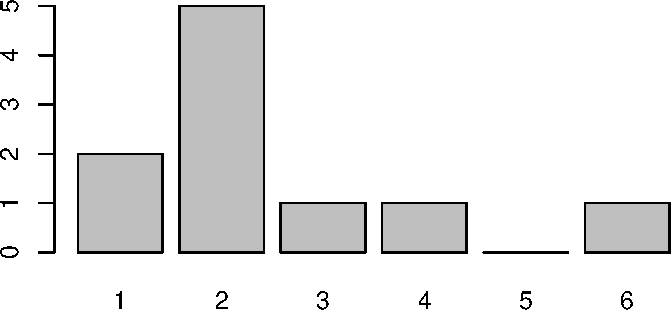
\includegraphics[keepaspectratio]{Lecture-10-Probability-Distributions_files/figure-pdf/unnamed-chunk-16-1.pdf}}

Notice how in the visualization above each outcome is not equally
represented. This is because when our sample size is small it will not
necessarily look like what we expect, but as the sample size increases
it looks closer and closer to the theoretical probability. To see this
we can visualize rolling 50 dice or even 10,000 dice:

\begin{Shaded}
\begin{Highlighting}[]
\NormalTok{x }\OtherTok{\textless{}{-}} \FunctionTok{sample}\NormalTok{(}\DecValTok{1}\SpecialCharTok{:}\DecValTok{6}\NormalTok{, }\DecValTok{50}\NormalTok{, }\AttributeTok{replace=}\ConstantTok{TRUE}\NormalTok{)}
\FunctionTok{table}\NormalTok{(x)}
\end{Highlighting}
\end{Shaded}

\begin{verbatim}
x
 1  2  3  4  5  6 
 7 15 10  6  4  8 
\end{verbatim}

\begin{Shaded}
\begin{Highlighting}[]
\FunctionTok{barplot}\NormalTok{(}\FunctionTok{table}\NormalTok{(x))}
\end{Highlighting}
\end{Shaded}

\pandocbounded{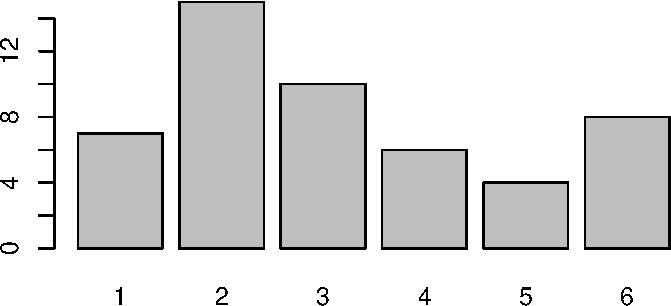
\includegraphics[keepaspectratio]{Lecture-10-Probability-Distributions_files/figure-pdf/unnamed-chunk-17-1.pdf}}

\begin{Shaded}
\begin{Highlighting}[]
\NormalTok{x }\OtherTok{\textless{}{-}} \FunctionTok{sample}\NormalTok{(}\DecValTok{1}\SpecialCharTok{:}\DecValTok{6}\NormalTok{, }\DecValTok{10000}\NormalTok{, }\AttributeTok{replace=}\ConstantTok{TRUE}\NormalTok{)}
\FunctionTok{table}\NormalTok{(x)}
\end{Highlighting}
\end{Shaded}

\begin{verbatim}
x
   1    2    3    4    5    6 
1628 1668 1685 1656 1629 1734 
\end{verbatim}

\begin{Shaded}
\begin{Highlighting}[]
\FunctionTok{barplot}\NormalTok{(}\FunctionTok{table}\NormalTok{(x))}
\end{Highlighting}
\end{Shaded}

\pandocbounded{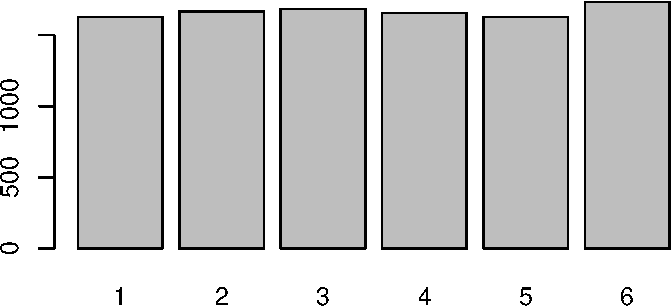
\includegraphics[keepaspectratio]{Lecture-10-Probability-Distributions_files/figure-pdf/unnamed-chunk-18-1.pdf}}

If all outcomes have an equal chance of occurring then the probability
is identical (uniform) for all possible outcomes. It can be modeled
using a \textbf{Uniform Discrete Distribution}. The probability
distribution can be described as:

\[ P(X=k)=\frac{1}{n}\]

where \(n\) is the number of possible outcomes. For this distribution,
the mean will be \(\mu=\frac{a+b}{2}\) (where \(a\) and \(b\) are the
``end-points'') and the standard deviation will be
\(\sigma=\sqrt{\frac{n^2-1}{12}}\). We will only really have to deal
with these if our outcomes are quantitative and sequential (or at least
evenly separated).

\begin{watch}{}{}
    \href{https://youtu.be/WWIZw8LfBI8}{Simulating a Uniform Discrete Distribution}
\end{watch}

\subsection{Poisson Distribution}\label{poisson-distribution}

The last discrete probability distribution we want to discuss is the
\textbf{Poisson Distribution}. This distribution will give us the
probability of a given number of events occurring in a fixed time
interval. This will only apply if the events occur at a constant rate
\(\lambda\) (pronounced ``lambda'') and the events are independent of
each other (meaning one occurrence does not affect another occurrence).
The probability distribution can be described as:
\[ \text{P(X=k)}=\frac{\lambda^ke^{-\lambda}}{k!}\]

with \(e\) being the mathematical constant \(2.71828\dots\). Some
properties of this distribution are that the mean is \(\mu=\lambda\) and
the standard deviation is \(\sigma = \sqrt{\lambda}\).

To create simulations for this distribution in R, we will use the
\emph{rpois()} function which generate random values from the Poisson
distribution. Similar functions exist for other distributions as well
(such as \emph{rbinom()} for random values from a binomial
distribution). Additional functions will allow us to calculate
theoretical probabilities in R using \(p\) instead of \(r\) at the front
of the function. We will discuss these in more detail during future
lectures.

Let's consider the following example: A considerable amount of
18-Wheelers drive down Emmitsburg's Main Street each day. If they come
through at a rate of 2 per 15 minutes, what would we expect to see the
distribution look like? What happens if the rate changes to 5 per 15
minutes?

\begin{Shaded}
\begin{Highlighting}[]
\NormalTok{x }\OtherTok{\textless{}{-}} \FunctionTok{rpois}\NormalTok{(}\DecValTok{10000}\NormalTok{,}\AttributeTok{lambda=}\DecValTok{2}\NormalTok{) }\CommentTok{\# Random values assuming 2 per 15{-}minutes}
\FunctionTok{table}\NormalTok{(x)}
\end{Highlighting}
\end{Shaded}

\begin{verbatim}
x
   0    1    2    3    4    5    6    7    8    9 
1336 2743 2676 1778  948  364  120   24    8    3 
\end{verbatim}

\begin{Shaded}
\begin{Highlighting}[]
\FunctionTok{barplot}\NormalTok{(}\FunctionTok{table}\NormalTok{(x))}
\end{Highlighting}
\end{Shaded}

\pandocbounded{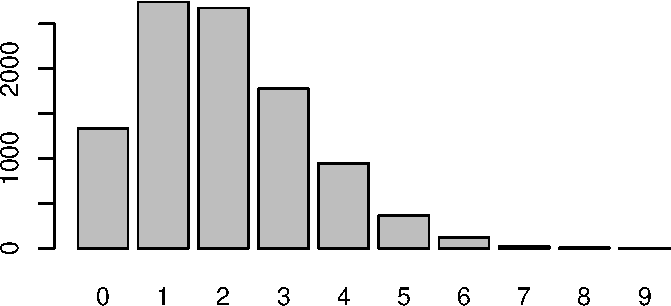
\includegraphics[keepaspectratio]{Lecture-10-Probability-Distributions_files/figure-pdf/unnamed-chunk-19-1.pdf}}

\begin{Shaded}
\begin{Highlighting}[]
\NormalTok{x }\OtherTok{\textless{}{-}} \FunctionTok{rpois}\NormalTok{(}\DecValTok{10000}\NormalTok{,}\AttributeTok{lambda=}\DecValTok{5}\NormalTok{) }\CommentTok{\# Random values assuming 5 per 15{-}minutes}
\FunctionTok{table}\NormalTok{(x)}
\end{Highlighting}
\end{Shaded}

\begin{verbatim}
x
   0    1    2    3    4    5    6    7    8    9   10   11   12   13   14   15 
  64  356  864 1417 1745 1764 1457 1033  632  366  153   94   35   14    4    1 
  16 
   1 
\end{verbatim}

\begin{Shaded}
\begin{Highlighting}[]
\FunctionTok{barplot}\NormalTok{(}\FunctionTok{table}\NormalTok{(x))}
\end{Highlighting}
\end{Shaded}

\pandocbounded{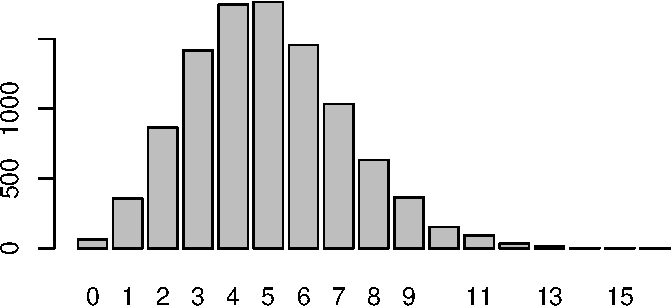
\includegraphics[keepaspectratio]{Lecture-10-Probability-Distributions_files/figure-pdf/unnamed-chunk-20-1.pdf}}

Altering the lambda will affect the distribution's shape. Below shows a
few different lambdas along with how the distribution will look

\begin{center}
\pandocbounded{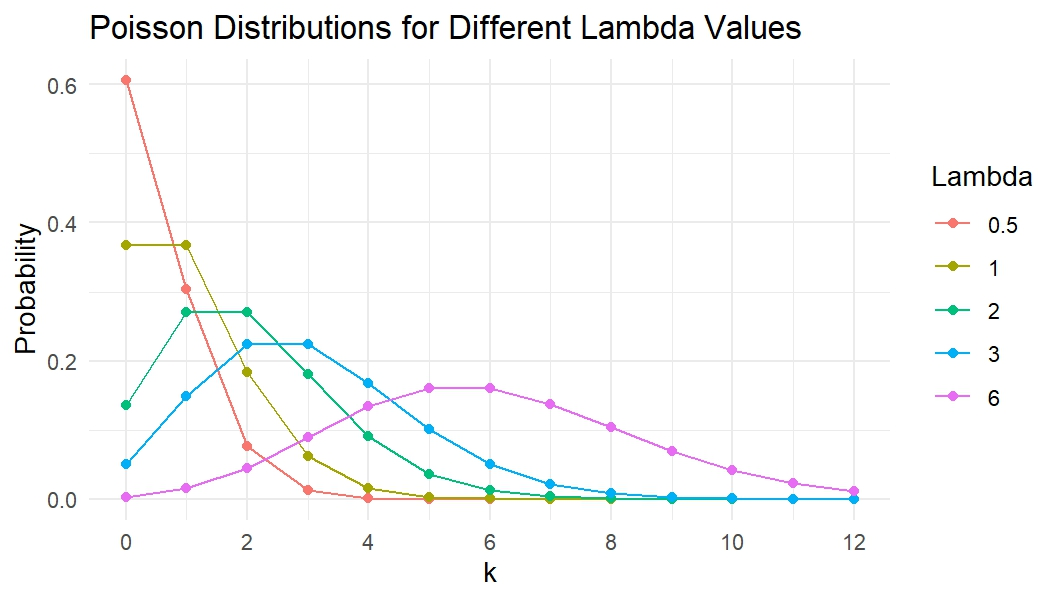
\includegraphics[keepaspectratio]{images/L10-Poisson-distribution-graph.png}}
\end{center}

Going back to the example, we can calculate the probability the 4 trucks
drive through town if the rate is 5 per 15 minutes. This can be done
both theoretically (the top example) and empirically (the bottom
example):

\begin{Shaded}
\begin{Highlighting}[]
\NormalTok{(}\DecValTok{5}\SpecialCharTok{\^{}}\DecValTok{4} \SpecialCharTok{*} \FunctionTok{exp}\NormalTok{(}\SpecialCharTok{{-}}\DecValTok{5}\NormalTok{))}\SpecialCharTok{/}\FunctionTok{factorial}\NormalTok{(}\DecValTok{4}\NormalTok{)}
\end{Highlighting}
\end{Shaded}

\begin{verbatim}
[1] 0.1754674
\end{verbatim}

\begin{Shaded}
\begin{Highlighting}[]
\DecValTok{1745}\SpecialCharTok{/}\DecValTok{10000}
\end{Highlighting}
\end{Shaded}

\begin{verbatim}
[1] 0.1745
\end{verbatim}

We could also find the Probability of seeing less than or equal to 4
18-Wheelers:

\begin{Shaded}
\begin{Highlighting}[]
\FunctionTok{sum}\NormalTok{(x}\SpecialCharTok{\textless{}=}\DecValTok{4}\NormalTok{)}\SpecialCharTok{/}\DecValTok{10000}
\end{Highlighting}
\end{Shaded}

\begin{verbatim}
[1] 0.4446
\end{verbatim}

\begin{watch}{}{}
    \href{https://youtu.be/RsaVDiUv5C0}{Simulating a Poisson Distribution}
\end{watch}

\section{Population, Sample, \& the Law of Large
Numbers}\label{population-sample-the-law-of-large-numbers}

Since we are coming to the end of the lecture on discrete probability
distributions, we should probably cover a few definitions that will pop
up throughout the rest of the course. The first is the difference
between a population and a sample. A \textbf{population} is the entire
collection of possible values for a measured observation, while a
\textbf{sample} is just the subset of the population that we collect.
For instance, if you are interested in the number of siblings all
college students have then your population would be all college students
while your sample is just the students you get data on.

The next definition we should discuss is a random variable. A
\textbf{random variable} is the value of an observation determined by a
chance event. For instance, rolling a die or flipping a coin would be a
random variable. A \textbf{Frequency Distribution} is the frequency of a
random variable occurring at all observed values. This will help us
calculate empirical probabilities and is an approximation for the
population distribution.

Lastly, we have seen throughout this lecture that as we increase the
sample size, the visualization looks closer and closer to what we would
expect. This is due to the \textbf{Law of Large Numbers}, which states
that as our sample gets larger and larger, the relative frequencies will
converge to the probability from the population distribution.

\section{Continuous Probability}\label{continuous-probability}

Last in this chapter we discussed some Discrete Distributions and were
able to calculate the probability that a single event occurred. We can
do a similar idea with continuous data except that instead of
calculating \(P(X=a)\), we will be calculating the probability of
falling within a range of values such as \(P(X<a)\) or
\(P(a\leq X \leq b)\). This should hopefully make sense as continuous
data can take on any value in a given interval, so the probability that
our backpack weighs exactly 6.4939 pounds is 0 since this is only 1
value with an infinite amount of possibilities if the scale can be
infinitely precise. For the students who have taken calculus before, we
(should) know that the integral at a single point, that is
\(\int_a^a f(x)\ dx\), is 0.

\subsection{Uniform Continuous
Distribution}\label{uniform-continuous-distribution}

The first distribution we will discuss is the \textbf{Uniform Continuous
Distribution}. Similar to the Uniform Discrete Distribution, all
possibilities within the interval \([a,b]\) have the same chance of
being selected. The visualization of this distribution is essentially
``flat'' across the specified interval. The Uniform Continuous
distribution can be described by the probability distribution
\(f(x)=\frac{1}{b-a}\) when \(a\leq x \leq b\) and \(f(x)=0\) otherwise.
The mean will be \(\mu=\frac{b+a}{2}\) and the standard deviation will
be \(\sigma = \sqrt{\frac{(b-a)^2}{12}}\)\textbackslash{}

Uniform Distributions occur when all of the ranges of outputs are
equally likely. People's heights typically are not uniformly distributed
(as most people are around 68 inches tall, with a few really short
people and a few tall people). But, if we look at the decimal values of
the height (for a person 68.283 inches tall if we just use the .283
portion) then that would be uniformly distributed. This idea of a
continuous Uniform distribution is also seen in Random Number
Generators, which are vital in simulations and computer applications!

The code to simulate a uniform continuous distribution in R is fairly
straightforward. We will use the \emph{runif()} function which requires
us to specify the number of random uniform numbers. We can also specify
the minimum and maximum values for the digits. If we do not specify this
then it will return values between 0 and 1. To view discrete data we
used a barplot, but if we want to view the continuous data then we
should utilize a histogram using the \emph{hist()} function.

\begin{Shaded}
\begin{Highlighting}[]
\FunctionTok{runif}\NormalTok{(}\DecValTok{5}\NormalTok{)}
\end{Highlighting}
\end{Shaded}

\begin{verbatim}
[1] 0.3039341 0.3271780 0.9936374 0.7228282 0.8854631
\end{verbatim}

\begin{Shaded}
\begin{Highlighting}[]
\FunctionTok{runif}\NormalTok{(}\DecValTok{5}\NormalTok{, }\AttributeTok{min=}\DecValTok{13}\NormalTok{, }\AttributeTok{max=}\DecValTok{15}\NormalTok{)}
\end{Highlighting}
\end{Shaded}

\begin{verbatim}
[1] 13.20895 14.21335 13.97186 13.69464 14.81628
\end{verbatim}

\begin{Shaded}
\begin{Highlighting}[]
\NormalTok{uniform\_data }\OtherTok{\textless{}{-}} \FunctionTok{runif}\NormalTok{(}\DecValTok{100}\NormalTok{, }\AttributeTok{min=}\DecValTok{0}\NormalTok{, }\AttributeTok{max=}\DecValTok{1}\NormalTok{)}
\FunctionTok{hist}\NormalTok{(uniform\_data, }\AttributeTok{col=}\StringTok{"lightblue"}\NormalTok{, }\AttributeTok{main=}\StringTok{"Uniform Distribution"}\NormalTok{, }
     \AttributeTok{breaks=}\DecValTok{20}\NormalTok{, }\AttributeTok{freq =} \ConstantTok{FALSE}\NormalTok{)}
\end{Highlighting}
\end{Shaded}

\pandocbounded{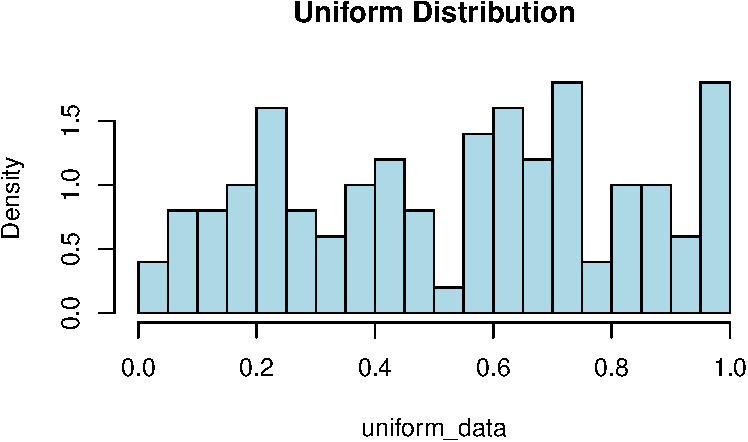
\includegraphics[keepaspectratio]{Lecture-10-Probability-Distributions_files/figure-pdf/unnamed-chunk-23-1.pdf}}

Now we might not have gotten a very Uniform looking visualization with
the code above, and that is because our sample of size 100 is relatively
small. The Law of Large Numbers tells us that as our sample grows larger
and larger, our distribution will get closer and closer to the expected
population distribution. So now try running the same code but change the
sample size from 100 to 100,000 and see how it looks more uniform.

\begin{Shaded}
\begin{Highlighting}[]
\NormalTok{uniform\_data }\OtherTok{\textless{}{-}} \FunctionTok{runif}\NormalTok{(}\DecValTok{100000}\NormalTok{, }\AttributeTok{min=}\DecValTok{0}\NormalTok{, }\AttributeTok{max=}\DecValTok{1}\NormalTok{)}
\FunctionTok{hist}\NormalTok{(uniform\_data, }\AttributeTok{col=}\StringTok{"lightblue"}\NormalTok{, }\AttributeTok{main=}\StringTok{"Uniform Distribution"}\NormalTok{, }
     \AttributeTok{breaks=}\DecValTok{20}\NormalTok{, }\AttributeTok{freq =} \ConstantTok{FALSE}\NormalTok{)}
\end{Highlighting}
\end{Shaded}

\pandocbounded{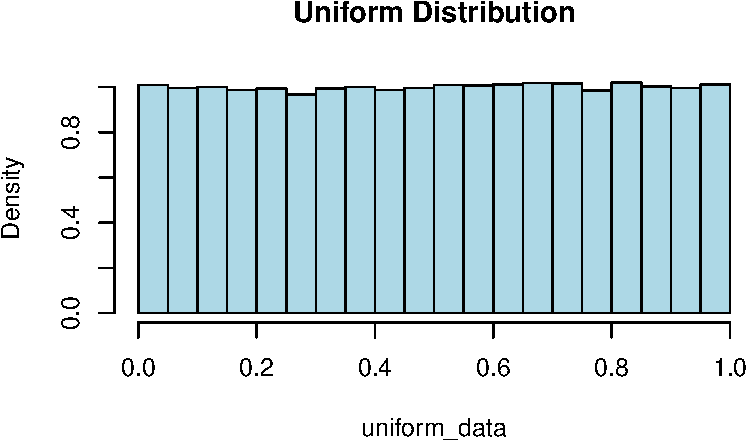
\includegraphics[keepaspectratio]{Lecture-10-Probability-Distributions_files/figure-pdf/unnamed-chunk-24-1.pdf}}

\begin{watch}{}{}
    \href{https://youtu.be/xgtVcr1Zj6g}{Simulating a Uniform Continuous Distribution}
\end{watch}

\subsection{Gamma Distribution}\label{gamma-distribution}

The \textbf{Gamma Distribution} is another continuous distribution that
has important aspects in the world of Data Science. This distribution
has values that are always positive and right-skewed (meaning we have an
outlier on the right side, making the ``tail'' longer). This
distribution is particularly useful in describing the time until the
\(n^{\text{th}}\) Poisson event. We will not worry about ``math'' of the
function, but we will note that the curve is defined by shape \(k\) and
scale \(\theta\). The mean will end up being \(\mu=k\theta\) and the
standard deviation will be \(\sigma=\sqrt{k\theta^2}\)

We should note that this distribution can be used for any data which we
anticipate will be skewed, and does not have to deal with just the time
until the \(n^{\text{th}}\) Poisson event. To simulate random values for
a gamma distribution we will use the \emph{rgamma()} function where we
can specify the number of values we want along with the shape, and
either the scale or rate (sometimes we might also mention rate which is
1/scale). The visualization below shows what the distribution may look
like. A density line has been drawn over the top of the histogram to
help visualize the distribution.

\begin{Shaded}
\begin{Highlighting}[]
\NormalTok{gamma\_data }\OtherTok{\textless{}{-}} \FunctionTok{rgamma}\NormalTok{(}\DecValTok{50}\NormalTok{, }\AttributeTok{shape=}\FloatTok{2.5}\NormalTok{, }\AttributeTok{scale=}\DecValTok{20000}\NormalTok{)}
\FunctionTok{hist}\NormalTok{(gamma\_data, }\AttributeTok{col=}\StringTok{"lightblue"}\NormalTok{, }\AttributeTok{main=}\StringTok{"Salary of Population"}\NormalTok{, }
     \AttributeTok{freq=}\ConstantTok{FALSE}\NormalTok{)}
\FunctionTok{lines}\NormalTok{(}\FunctionTok{density}\NormalTok{(gamma\_data), }\AttributeTok{col=}\StringTok{"red"}\NormalTok{, }\AttributeTok{lwd=}\DecValTok{2}\NormalTok{)}
\end{Highlighting}
\end{Shaded}

\pandocbounded{\includegraphics[keepaspectratio]{Lecture-10-Probability-Distributions_files/figure-pdf/unnamed-chunk-25-1.pdf}}

Every time you run the code above you may get vastly different-looking
graphs, which is due to the small sample size of our data. The Law of
Large Numbers (wow\ldots second time it has been mentioned, it must be
important\ldots) tells us that we need a large sample for it to look
like a ``smooth'' distribution. If we have a relatively small sample
then we cannot guarantee it will look ``nice''. The visualization below
shows how the shape and scale affect the look of the distribution:

\pandocbounded{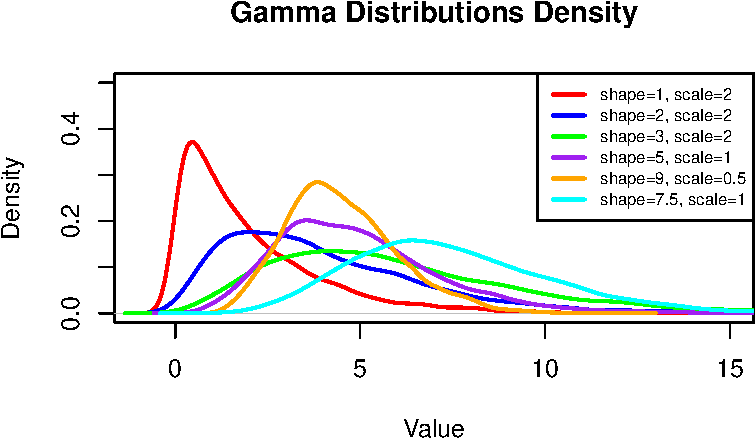
\includegraphics[keepaspectratio]{Lecture-10-Probability-Distributions_files/figure-pdf/unnamed-chunk-26-1.pdf}}

\begin{watch}{}{}
    \href{https://youtu.be/yjm4U70TXh8}{Simulating a Gamma Distribution}
\end{watch}

\subsection{Exponential Distribution}\label{exponential-distribution}

The \textbf{Exponential Distribution} is going to be similar to the
Gamma Distribution with one slight caveat, it is the time between
Poisson events and not the time until the \(n^{\text{th}}\) event. This
is often referred to as a memory-less distribution as we start over each
time we see an observation and count the time til the next one. So, the
Exponential Distribution is a special case of the Gamma distribution
when the shape is 1 and the scale is \(\frac{1}{\lambda}\). The mean and
standard deviation for this distribution will be
\(\mu=\sigma=\frac{1}{\lambda}\).

This is useful when we are interested in determining the arrival time
between events. If we go back to our example of 18-wheelers driving down
Main Street at a rate of 4 per 15 minutes, we can determine the time
between the 18-wheelers coming through the city.

\begin{Shaded}
\begin{Highlighting}[]
\NormalTok{exp\_data }\OtherTok{\textless{}{-}} \FunctionTok{rexp}\NormalTok{(}\DecValTok{50}\NormalTok{, }\AttributeTok{rate=}\DecValTok{4}\NormalTok{)}
\FunctionTok{hist}\NormalTok{(exp\_data, }\AttributeTok{col=}\StringTok{"lightblue"}\NormalTok{, }\AttributeTok{main=}\StringTok{"Exponential Distribution"}\NormalTok{, }
     \AttributeTok{xlab=}\StringTok{"Time Between 18{-}Wheelers"}\NormalTok{, }\AttributeTok{breaks=}\DecValTok{20}\NormalTok{, }\AttributeTok{freq=}\ConstantTok{FALSE}\NormalTok{)}
\FunctionTok{lines}\NormalTok{(}\FunctionTok{density}\NormalTok{(exp\_data), }\AttributeTok{col=}\StringTok{"red"}\NormalTok{)}
\end{Highlighting}
\end{Shaded}

\pandocbounded{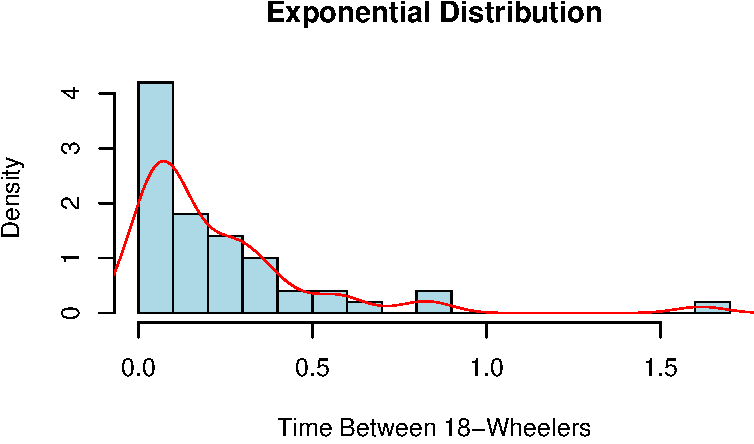
\includegraphics[keepaspectratio]{Lecture-10-Probability-Distributions_files/figure-pdf/unnamed-chunk-27-1.pdf}}

Once again, this probably does not look very nice or smooth as we have
relatively few pieces of data visualized. I encourage you to try the
code above again but this time change the number of observations in the
sample from 50 to 5,000 and see how different it looks. We could also
rewrite the rate to alter the units. Currently, it is 4 per 15 minutes,
but we could also have it as \(4\times4=16\) for 16 every hour or even
\(4/15\) for the amount per minute. This would change the units on the
x-axis to whatever units the rate is in.

\begin{Shaded}
\begin{Highlighting}[]
\NormalTok{exp\_data }\OtherTok{\textless{}{-}} \FunctionTok{rexp}\NormalTok{(}\DecValTok{1000}\NormalTok{, }\AttributeTok{rate=}\DecValTok{4}\SpecialCharTok{/}\DecValTok{15}\NormalTok{)}
\FunctionTok{hist}\NormalTok{(exp\_data, }\AttributeTok{col=}\StringTok{"lightblue"}\NormalTok{, }\AttributeTok{main=}\StringTok{"Exponential Distribution"}\NormalTok{, }
     \AttributeTok{xlab=}\StringTok{"Time Between 18{-}Wheelers"}\NormalTok{, }\AttributeTok{breaks=}\DecValTok{20}\NormalTok{, }\AttributeTok{freq=}\ConstantTok{FALSE}\NormalTok{)}
\FunctionTok{lines}\NormalTok{(}\FunctionTok{density}\NormalTok{(exp\_data), }\AttributeTok{col=}\StringTok{"red"}\NormalTok{)}
\end{Highlighting}
\end{Shaded}

\pandocbounded{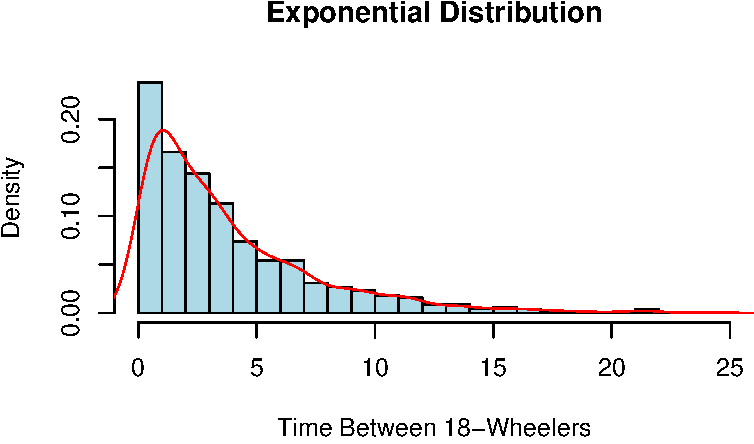
\includegraphics[keepaspectratio]{Lecture-10-Probability-Distributions_files/figure-pdf/unnamed-chunk-28-1.pdf}}

\begin{watch}{}{}
    \href{https://youtu.be/ovC6V7MzD6U}{Simulating an Exponential Distribution}
\end{watch}

\subsection{Normal Distribution}\label{normal-distribution}

We will see that many characteristics in nature follow what we call the
\textbf{Normal Distribution}. This is a uni-modal (one hump) symmetric
distribution centered around the mean with the shape dependent on the
standard deviation. You have probably heard people refer to the ``bell''
curve before since it tends to resemble the shape of a bell.
Characteristics such as heights, grades, stock market returns, blood
pressure, and many more things follow this distribution. It can be
described by its mean \(\mu\) and the standard deviation \(\sigma\),
both of which are arguments that we can decide.

This is one of the most important distributions in statistics, as we
will be revisiting this distribution continually throughout the rest of
the semester. Later on, we will see why it is so important and how it
relates to arguably one of the Top 3 Most Influential Theorems (the
Central Limit Theorem). We can see the distribution at work if we want
to look at the average height of students. We will assume the average
height is 68 inches while the standard deviation is 3 inches.

\begin{Shaded}
\begin{Highlighting}[]
\NormalTok{normal\_data }\OtherTok{\textless{}{-}} \FunctionTok{rnorm}\NormalTok{(}\DecValTok{100}\NormalTok{, }\AttributeTok{mean=}\DecValTok{68}\NormalTok{, }\AttributeTok{sd=}\DecValTok{3}\NormalTok{)}
\FunctionTok{hist}\NormalTok{(normal\_data, }\AttributeTok{col=}\StringTok{"lightblue"}\NormalTok{, }\AttributeTok{main=}\StringTok{"Height of Students"}\NormalTok{, }
     \AttributeTok{breaks=}\DecValTok{20}\NormalTok{, }\AttributeTok{freq=}\ConstantTok{FALSE}\NormalTok{)}
\FunctionTok{lines}\NormalTok{(}\FunctionTok{density}\NormalTok{(normal\_data), }\AttributeTok{col=}\StringTok{"red"}\NormalTok{, }\AttributeTok{lwd=}\DecValTok{2}\NormalTok{)}
\end{Highlighting}
\end{Shaded}

\pandocbounded{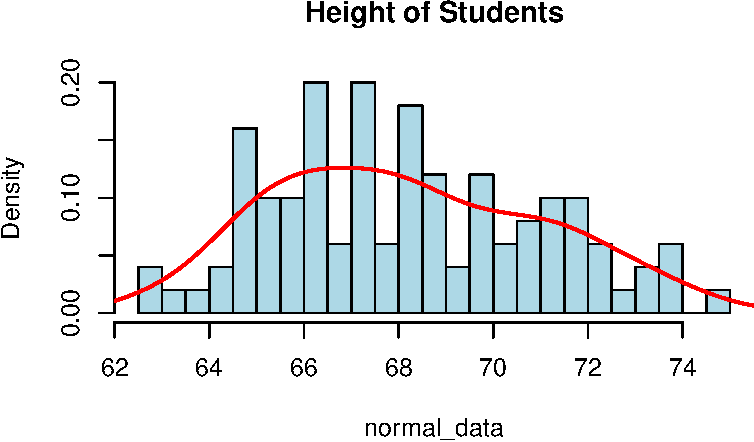
\includegraphics[keepaspectratio]{Lecture-10-Probability-Distributions_files/figure-pdf/unnamed-chunk-29-1.pdf}}

Once again, if we increase the sample size, it will look more and more
smooth due to the Law of Large Numbers (another very important and
influential theorem). There are a lot of neat properties that come from
the Normal Distribution, one of which is called the 68-95-99.7 Rule.
This states that roughly 68\% of our data falls within 1 standard
deviation of the mean, 95\% of our data falls within 2 standard
deviations of the mean, and 99.7\% of our data falls within 3 standard
deviations of the mean.

Given the normally distributed data that we created above, we could test
this idea and see if the 68-95-99.7 Rule does hold up. The following
code is an example of how we may see it. Note that you may get different
results due to the fact you will be generating a different random sample
than I have. I will increase the sample size to 1000 to get more
accurate results.

\begin{Shaded}
\begin{Highlighting}[]
\NormalTok{normal\_data }\OtherTok{\textless{}{-}} \FunctionTok{rnorm}\NormalTok{(}\DecValTok{1000}\NormalTok{, }\AttributeTok{mean=}\DecValTok{68}\NormalTok{, }\AttributeTok{sd=}\DecValTok{3}\NormalTok{)}
\FunctionTok{mean}\NormalTok{(normal\_data)}
\end{Highlighting}
\end{Shaded}

\begin{verbatim}
[1] 68.0472
\end{verbatim}

\begin{Shaded}
\begin{Highlighting}[]
\FunctionTok{sd}\NormalTok{(normal\_data)}
\end{Highlighting}
\end{Shaded}

\begin{verbatim}
[1] 3.007
\end{verbatim}

\begin{Shaded}
\begin{Highlighting}[]
\FunctionTok{hist}\NormalTok{(normal\_data, }\AttributeTok{col=}\StringTok{"lightblue"}\NormalTok{, }\AttributeTok{main=}\StringTok{"Height of Students"}\NormalTok{, }
     \AttributeTok{breaks=}\DecValTok{20}\NormalTok{, }\AttributeTok{freq=}\ConstantTok{FALSE}\NormalTok{)}
\FunctionTok{lines}\NormalTok{(}\FunctionTok{density}\NormalTok{(normal\_data), }\AttributeTok{col=}\StringTok{"red"}\NormalTok{)}
\end{Highlighting}
\end{Shaded}

\pandocbounded{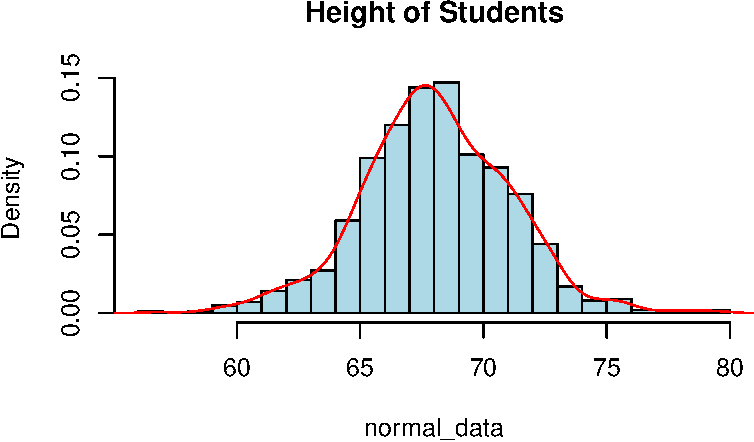
\includegraphics[keepaspectratio]{Lecture-10-Probability-Distributions_files/figure-pdf/unnamed-chunk-30-1.pdf}}

\begin{Shaded}
\begin{Highlighting}[]
\FunctionTok{sum}\NormalTok{(normal\_data }\SpecialCharTok{\textgreater{}} \FunctionTok{mean}\NormalTok{(normal\_data) }\SpecialCharTok{{-}} \FunctionTok{sd}\NormalTok{(normal\_data) }\SpecialCharTok{\&} 
\NormalTok{      normal\_data }\SpecialCharTok{\textless{}} \FunctionTok{mean}\NormalTok{(normal\_data) }\SpecialCharTok{+} \FunctionTok{sd}\NormalTok{(normal\_data))}\SpecialCharTok{/}\DecValTok{1000}
\end{Highlighting}
\end{Shaded}

\begin{verbatim}
[1] 0.706
\end{verbatim}

\begin{Shaded}
\begin{Highlighting}[]
\FunctionTok{sum}\NormalTok{(normal\_data }\SpecialCharTok{\textgreater{}} \FunctionTok{mean}\NormalTok{(normal\_data) }\SpecialCharTok{{-}} \DecValTok{2}\SpecialCharTok{*}\FunctionTok{sd}\NormalTok{(normal\_data) }\SpecialCharTok{\&} 
\NormalTok{      normal\_data }\SpecialCharTok{\textless{}} \FunctionTok{mean}\NormalTok{(normal\_data) }\SpecialCharTok{+} \DecValTok{2}\SpecialCharTok{*}\FunctionTok{sd}\NormalTok{(normal\_data))}\SpecialCharTok{/}\DecValTok{1000}
\end{Highlighting}
\end{Shaded}

\begin{verbatim}
[1] 0.947
\end{verbatim}

So with this, we can see that the 68-95-99.7 rule is pretty accurate in
telling us what percentage of the data is within so many standard
deviations of the mean. You should get similar, but slightly different
results. The more data in your sample the closer you will be to the true
proportion.

\begin{watch}{}{}
    \href{https://youtu.be/0C7qVM9wr3c}{Simulating a Normal Distribution}
\end{watch}

\bookmarksetup{startatroot}

\chapter{Describing a Distribution}\label{describing-a-distribution}

\section{Center Statistics}\label{center-statistics}

We have already done some Exploratory Data Analysis (EDA) in order to
become familiar with the data. We asked ourselves what the logical and
physical structure were, as well as if there were any ``issues'' with
the data concerning missing values. We also started to prepare the data
for future analysis by converting some columns to factors and
occasionally creating new factor columns using the \emph{cut()} function
on a column composed of quantitative data. We finished off our Goal 1 of
EDA by looking at a summary of the dataset and visualizing it in order
to get a better idea of what the data we were working with looks like.

Now that we are familiar with the dataset and know what it looks like,
we can move on to describing the data. To describe the data, we can use
\textbf{descriptive statistics}. The three of the big ways we will use
to describe a dataset are the center, the spread, and the shape of the
dataset. All of these will help us understand the data at a deeper
level.

\subsection{Measures of Central
Tendency}\label{measures-of-central-tendency}

Describing the center of a dataset can help give us insight into what
the data looks like, but we do lose some meaning when we reduce all of
the data values down to a single representative value. Because we lose
some meaning, multiple ``competing'' definitions of the center have
emerged. These different definitions will allow us to identify patterns
in the data that a single one by itself will not be able to tell us. We
already know that there are multiple different ways in which we can
describe the center of a dataset. We can do this with the \textbf{mean},
which is the average, the \textbf{median}, which is the middle of a
sorted list, and the \textbf{mode}, which is where the highest occurring
frequency happens.

The central tendency can give us insight into the shape of the
distribution. In order for a distribution to be symmetric, that is the
``left-hand'' side and the ``right-hand'' side look like mirror images,
the mean must equal the median. This is a necessary condition, but not
necessarily a sufficient condition. If the mean and median are equal
then do we have a symmetric distribution? We will investigate this
condition later after we look into the shape and spread of the
distribution a little bit more.

\begin{center}
\pandocbounded{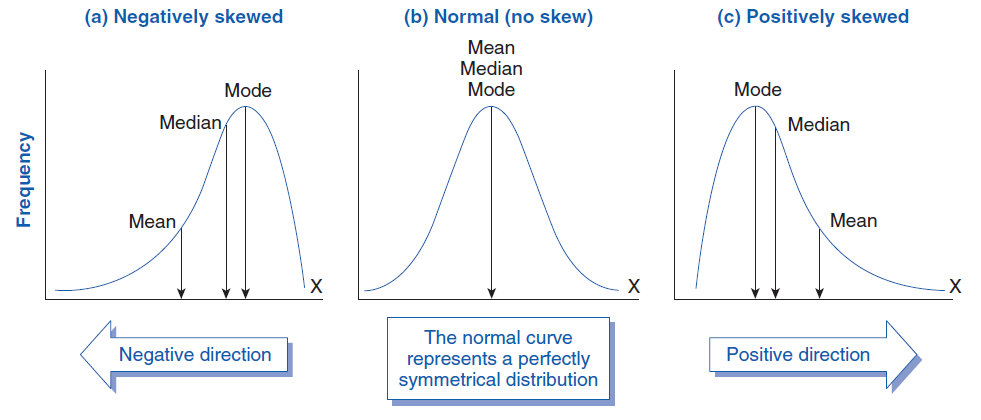
\includegraphics[keepaspectratio]{images/L11-skewed-distributions.png}}
\end{center}

\subsection{Quartile Analysis}\label{quartile-analysis}

Let's look at a quick example in order to see how the center can tell us
about the shape. The first thing that we will probably want to look at
is to see if the mean and median are close to each other. Then, another
thing we can do is look at the Quartiles of the dataset. We will want to
see if the range of the \(2^{\text{nd}}\) Quartile (2Q) and the
\(3^{\text{rd}}\) Quartile (3Q) are comparable as well as if the range
of the \(1^{\text{st}}\) Quartile (1Q) and \(4^{\text{th}}\) Quartile
(4Q) are comparable. If the range of the \(1^{\text{st}}\) Quartile is
much larger than the range of the \(4^{\text{th}}\) Quartile then it may
indicate that the distribution is negatively skewed. Now, remember that
the \(1^{\text{st}}\) Quartile is the first 25\% of the data, the
\(2^{\text{nd}}\) Quartile is the second 25\% of the data, and so on.

\begin{center}
\pandocbounded{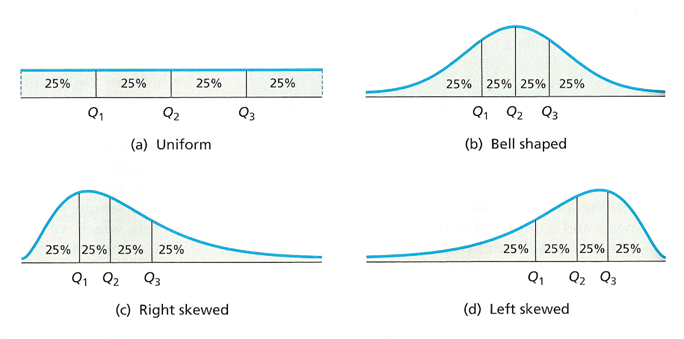
\includegraphics[keepaspectratio]{images/L11-skewed-quartiles.png}}
\end{center}

\begin{Shaded}
\begin{Highlighting}[]
\FunctionTok{summary}\NormalTok{(iris}\SpecialCharTok{$}\NormalTok{Sepal.Length)}
\end{Highlighting}
\end{Shaded}

\begin{verbatim}
   Min. 1st Qu.  Median    Mean 3rd Qu.    Max. 
  4.300   5.100   5.800   5.843   6.400   7.900 
\end{verbatim}

In the output above, we can see that the mean and median are comparable
to each other, which indicates we might have a symmetric distribution.
Looking at the range of the \(2^{\text{nd}}\) and \(3^{\text{rd}}\)
Quartiles we can see the range of the \(3^{\text{rd}}\) Quartile
(\(6.4-5.8=0.6\)) is slightly smaller than the range of the
\(2^{\text{nd}}\) Quartile (\(5.8-5.1=0.7\)). Additionally, looking at
the range of the \(1^{\text{st}}\) Quartile (\(0.8\)) and
\(4^{\text{th}}\) Quartile (\(1.5\)) we can see that we have a wider Q4
then we have with Q1. This might indicate a positive skew since the
larger range of Q4 might suggest we have outliers above the mean.

Looking at another example, our first impression may be that the data is
slightly negatively skewed due to outliers below the mean. This is
because while the mean and median are similar, the range of Q1 is larger
than the range of Q4.

\begin{Shaded}
\begin{Highlighting}[]
\FunctionTok{summary}\NormalTok{(cars}\SpecialCharTok{$}\NormalTok{speed)}
\end{Highlighting}
\end{Shaded}

\begin{verbatim}
   Min. 1st Qu.  Median    Mean 3rd Qu.    Max. 
    4.0    12.0    15.0    15.4    19.0    25.0 
\end{verbatim}

We should note that this method is only to give us an initial impression
of the skew of the data and is not meant to be a definitive statement.
We will see additional techniques later that we can employ to get a more
definitive answer.

\subsection{Trimmed Mean}\label{trimmed-mean}

Another technique we can use to measure the central tendency is to use
the trimmed mean. It is important to remember that the mean is affected
by outliers, meaning extreme values on either side may cause the mean to
be ``pulled'' one way or another. The idea behind the trimmed is to
remove a percentage of the top and bottom values and then calculate the
mean. This allows us to determine the average of the majority of the
values, so the extreme outlier will not have any influence. This method
of finding the mean is used in many Olympic competitions, most notably
in Figure Skating. The highest and lowest scores are discarded so a
single judge could not ``tank'' the score of an opposing country's
competitor.

After carrying out a trimmed mean, the shift in the mean will highlight
the effect and impact of extreme values. If there is an increase with
the trimmed mean then it indicates we have extreme values on the
left-side. If there is a decrease with the trimmed mean then we have
outliers on the right-side. And if there is only a slight change then
there is only a minimal impact from extreme values.

This can be done in R using the `trim' argument within the mean
function. Below are a few examples of trimming 10\% in total (which does
5\% from both sides). The first example indicates that there are a few
extreme outliers above the mean which ``pull'' the mean up:

\begin{Shaded}
\begin{Highlighting}[]
\FunctionTok{mean}\NormalTok{(mtcars}\SpecialCharTok{$}\NormalTok{disp)}
\end{Highlighting}
\end{Shaded}

\begin{verbatim}
[1] 230.7219
\end{verbatim}

\begin{Shaded}
\begin{Highlighting}[]
\FunctionTok{mean}\NormalTok{(mtcars}\SpecialCharTok{$}\NormalTok{disp, }\AttributeTok{trim=}\NormalTok{.}\DecValTok{1}\NormalTok{)}
\end{Highlighting}
\end{Shaded}

\begin{verbatim}
[1] 222.5231
\end{verbatim}

In this next example we can see that the mean and the trimmed mean are
close to each other. This indicates that there is minimal impact from
outliers. It does not indicate that there are no outliers though, as the
outliers could be ``counter-acting'' each other.

\begin{Shaded}
\begin{Highlighting}[]
\FunctionTok{mean}\NormalTok{(iris}\SpecialCharTok{$}\NormalTok{Sepal.Length)}
\end{Highlighting}
\end{Shaded}

\begin{verbatim}
[1] 5.843333
\end{verbatim}

\begin{Shaded}
\begin{Highlighting}[]
\FunctionTok{mean}\NormalTok{(iris}\SpecialCharTok{$}\NormalTok{Sepal.Length, }\AttributeTok{trim=}\NormalTok{.}\DecValTok{1}\NormalTok{)}
\end{Highlighting}
\end{Shaded}

\begin{verbatim}
[1] 5.808333
\end{verbatim}

Finally, in this last example we can see the effect of an outlier on the
``left-hand'' side. The combine function is used to calculate the mean
of the Sepal.Length vector and the value -100. Doing the trimmed mean
removes this outlier and calculates the mean again, which indicates this
outlier on the ``left-hand'' side was affecting the mean.

\begin{Shaded}
\begin{Highlighting}[]
\FunctionTok{mean}\NormalTok{(}\FunctionTok{c}\NormalTok{(iris}\SpecialCharTok{$}\NormalTok{Sepal.Length,}\SpecialCharTok{{-}}\DecValTok{100}\NormalTok{))}
\end{Highlighting}
\end{Shaded}

\begin{verbatim}
[1] 5.142384
\end{verbatim}

\begin{Shaded}
\begin{Highlighting}[]
\FunctionTok{mean}\NormalTok{(}\FunctionTok{c}\NormalTok{(iris}\SpecialCharTok{$}\NormalTok{Sepal.Length,}\SpecialCharTok{{-}}\DecValTok{100}\NormalTok{), }\AttributeTok{trim=}\NormalTok{.}\DecValTok{1}\NormalTok{)}
\end{Highlighting}
\end{Shaded}

\begin{verbatim}
[1] 5.8
\end{verbatim}

\subsection{Weighted Mean}\label{weighted-mean}

Another important way to calculate the mean is using a weighted average.
The idea behind this calculation is to assign a weight to each value and
then calculate the mean. This is commonly done with quantitative
discrete data. You have used the weighted mean before to calculate your
grade grades and your GPA. The weighted mean can be described with the
following formula:
\[ \frac{\sum_{i=1}^n w_i\cdot x_i}{\sum_{i=1}^n w_i} \] where \(x_i\)
is the value and \(w_i\) is the weight associated with it.

When every value has the same weight then we are calculating the mean.
Below is an example of this:

\begin{Shaded}
\begin{Highlighting}[]
\NormalTok{x }\OtherTok{\textless{}{-}} \FunctionTok{c}\NormalTok{(}\DecValTok{1}\NormalTok{, }\DecValTok{4}\NormalTok{, }\DecValTok{7}\NormalTok{, }\DecValTok{4}\NormalTok{, }\DecValTok{5}\NormalTok{, }\DecValTok{9}\NormalTok{)}
\NormalTok{w }\OtherTok{\textless{}{-}} \FunctionTok{c}\NormalTok{(}\DecValTok{1}\SpecialCharTok{/}\DecValTok{2}\NormalTok{, }\DecValTok{1}\SpecialCharTok{/}\DecValTok{2}\NormalTok{, }\DecValTok{1}\SpecialCharTok{/}\DecValTok{2}\NormalTok{, }\DecValTok{1}\SpecialCharTok{/}\DecValTok{2}\NormalTok{, }\DecValTok{1}\SpecialCharTok{/}\DecValTok{2}\NormalTok{, }\DecValTok{1}\SpecialCharTok{/}\DecValTok{2}\NormalTok{)}

\FunctionTok{sum}\NormalTok{(x}\SpecialCharTok{*}\NormalTok{w)}\SpecialCharTok{/}\FunctionTok{sum}\NormalTok{(w)}
\end{Highlighting}
\end{Shaded}

\begin{verbatim}
[1] 5
\end{verbatim}

\begin{Shaded}
\begin{Highlighting}[]
\FunctionTok{mean}\NormalTok{(x)}
\end{Highlighting}
\end{Shaded}

\begin{verbatim}
[1] 5
\end{verbatim}

If the weights are different then it may not result in the mean of the
values. Below is an example of the weighted mean when it comes to
calculating final grades in the class:

\begin{Shaded}
\begin{Highlighting}[]
\NormalTok{x }\OtherTok{\textless{}{-}} \FunctionTok{c}\NormalTok{(}\DecValTok{90}\NormalTok{, }\DecValTok{100}\NormalTok{, }\DecValTok{70}\NormalTok{, }\DecValTok{50}\NormalTok{, }\DecValTok{95}\NormalTok{)}
\NormalTok{w }\OtherTok{\textless{}{-}} \FunctionTok{c}\NormalTok{(.}\DecValTok{05}\NormalTok{, .}\DecValTok{10}\NormalTok{, .}\DecValTok{25}\NormalTok{, .}\DecValTok{25}\NormalTok{, .}\DecValTok{35}\NormalTok{)}
\FunctionTok{mean}\NormalTok{(x)}
\end{Highlighting}
\end{Shaded}

\begin{verbatim}
[1] 81
\end{verbatim}

\begin{Shaded}
\begin{Highlighting}[]
\FunctionTok{sum}\NormalTok{(x}\SpecialCharTok{*}\NormalTok{w)}\SpecialCharTok{/}\FunctionTok{sum}\NormalTok{(w)}
\end{Highlighting}
\end{Shaded}

\begin{verbatim}
[1] 77.75
\end{verbatim}

Finally, we will look at a financial based question. Assuming that we
own a store which sells only 3 products: A for \$6.50, B for \$7.00, and
C for \$12. We might want to ask ourselves what the average sale price
is? Well, if we just took the mean of the three products we would get
\$8.50. But this does not take into account the fact that we might sell
more of one product than another. If we sold 200 units of Product A, 100
units of Product B, and only 5 units of Product C, then the average sale
price would be vastly different.

\begin{Shaded}
\begin{Highlighting}[]
\NormalTok{price }\OtherTok{\textless{}{-}} \FunctionTok{c}\NormalTok{(}\FloatTok{6.50}\NormalTok{, }\FloatTok{7.00}\NormalTok{, }\FloatTok{12.00}\NormalTok{)}
\FunctionTok{mean}\NormalTok{(price)}
\end{Highlighting}
\end{Shaded}

\begin{verbatim}
[1] 8.5
\end{verbatim}

\begin{Shaded}
\begin{Highlighting}[]
\NormalTok{sold }\OtherTok{\textless{}{-}} \FunctionTok{c}\NormalTok{(}\DecValTok{200}\NormalTok{,}\DecValTok{100}\NormalTok{,}\DecValTok{5}\NormalTok{)}
\FunctionTok{sum}\NormalTok{(price}\SpecialCharTok{*}\NormalTok{sold)}\SpecialCharTok{/}\FunctionTok{sum}\NormalTok{(sold)}
\end{Highlighting}
\end{Shaded}

\begin{verbatim}
[1] 6.754098
\end{verbatim}

\subsection{Mode}\label{mode}

The mode is another descriptive statistic which might be useful in
summarizing the data. This tells us which value occurs most frequently
in a dataset. Unfortunately, there is no function in base R which
calculates this for us, as the `\(mode()\)' function deals with the
storage of an object and does not calculate the value occurring most
frequently. We could create our own function in R in order to calculate
it though:

\begin{Shaded}
\begin{Highlighting}[]
\NormalTok{MODE }\OtherTok{\textless{}{-}} \ControlFlowTok{function}\NormalTok{(x)\{}
\NormalTok{     tbl }\OtherTok{\textless{}{-}} \FunctionTok{table}\NormalTok{(x)}
     \FunctionTok{as.numeric}\NormalTok{(}\FunctionTok{names}\NormalTok{(tbl[tbl}\SpecialCharTok{==}\FunctionTok{max}\NormalTok{(tbl)]))}
\NormalTok{     \}}
\end{Highlighting}
\end{Shaded}

\textbf{Note}: We will introduce a few functions in R over the next few
sections. You should be focused on when to use them and how to interpret
the output, not the actual code.

What the function above is doing is allowing us to pass a vector into
the function and it is then creating a table of all of the different
values. It then identifies which value in the table is the largest and
searches the table for any values that are equal to this value (since
there can be multiple modes). It then selects all of them that are the
maximum value and prints out the names of the selected values. Below is
an example to see the function at work:

\begin{Shaded}
\begin{Highlighting}[]
\FunctionTok{table}\NormalTok{(mtcars}\SpecialCharTok{$}\NormalTok{cyl)}
\end{Highlighting}
\end{Shaded}

\begin{verbatim}

 4  6  8 
11  7 14 
\end{verbatim}

\begin{Shaded}
\begin{Highlighting}[]
\FunctionTok{MODE}\NormalTok{(mtcars}\SpecialCharTok{$}\NormalTok{cyl)}
\end{Highlighting}
\end{Shaded}

\begin{verbatim}
[1] 8
\end{verbatim}

Our function will also be able to determine the mode if there are
multiple occurrences of the largest value:

\begin{Shaded}
\begin{Highlighting}[]
\NormalTok{data\_example }\OtherTok{\textless{}{-}} \FunctionTok{c}\NormalTok{(}\DecValTok{10}\NormalTok{, }\DecValTok{10}\NormalTok{, }\DecValTok{10}\NormalTok{, }\DecValTok{12}\NormalTok{, }\DecValTok{13}\NormalTok{, }\DecValTok{13}\NormalTok{, }\DecValTok{14}\NormalTok{, }\DecValTok{15}\NormalTok{, }\DecValTok{15}\NormalTok{, }\DecValTok{15}\NormalTok{, }\DecValTok{16}\NormalTok{, }\DecValTok{16}\NormalTok{, }\DecValTok{17}\NormalTok{)}
\FunctionTok{table}\NormalTok{(data\_example)}
\end{Highlighting}
\end{Shaded}

\begin{verbatim}
data_example
10 12 13 14 15 16 17 
 3  1  2  1  3  2  1 
\end{verbatim}

\begin{Shaded}
\begin{Highlighting}[]
\FunctionTok{MODE}\NormalTok{(data\_example)}
\end{Highlighting}
\end{Shaded}

\begin{verbatim}
[1] 10 15
\end{verbatim}

The function that we created only works for quantitative discrete data
though. Continuous data has too few repeats due to the values being able
to be anything within a given interval. This would result in our
function identifying every value as the mode, which is not very helpful.
We could use our density function to estimate the mode though. This
would tell us which value on our density function is the highest. Below
is the code for that (again, it is not vital for us to understand how to
write functions in R right now):

\begin{Shaded}
\begin{Highlighting}[]
\NormalTok{estimate\_mode }\OtherTok{\textless{}{-}} \ControlFlowTok{function}\NormalTok{(x) \{}
\NormalTok{     from}\OtherTok{=}\FunctionTok{min}\NormalTok{(x, }\AttributeTok{na.rm=}\ConstantTok{TRUE}\NormalTok{)}
\NormalTok{     to}\OtherTok{=}\FunctionTok{max}\NormalTok{(x, }\AttributeTok{na.rm=}\ConstantTok{TRUE}\NormalTok{)}
\NormalTok{     d }\OtherTok{\textless{}{-}} \FunctionTok{density}\NormalTok{(x, }\AttributeTok{from=}\NormalTok{from, }\AttributeTok{to=}\NormalTok{to, }\AttributeTok{na.rm=}\ConstantTok{TRUE}\NormalTok{)}
\NormalTok{     d}\SpecialCharTok{$}\NormalTok{x[}\FunctionTok{which.max}\NormalTok{(d}\SpecialCharTok{$}\NormalTok{y)]}
\NormalTok{     \}}
\end{Highlighting}
\end{Shaded}

If we were to randomly generate 1,000 observations from the normal
distribution and plot it we could see the density plot is largest around
53. The estimated mode tells us the density line is the tallest around
52.8, which confirms our visualization. The black vertical line was
inputted to help show where 52.8 was in the graph. We should be careful
in using our function, as it only works for continuous data with a
single peak. If we have bi-modal data (with 2 peaks) then we would have
to create a new function.

\begin{Shaded}
\begin{Highlighting}[]
\NormalTok{x }\OtherTok{\textless{}{-}} \FunctionTok{rnorm}\NormalTok{(}\DecValTok{1000}\NormalTok{,}\DecValTok{50}\NormalTok{,}\DecValTok{8}\NormalTok{)}
\FunctionTok{estimate\_mode}\NormalTok{(x)}
\end{Highlighting}
\end{Shaded}

\begin{verbatim}
[1] 50.01535
\end{verbatim}

\begin{Shaded}
\begin{Highlighting}[]
\FunctionTok{hist}\NormalTok{(x, }\AttributeTok{col=}\StringTok{"lightblue"}\NormalTok{, }\AttributeTok{freq=}\ConstantTok{FALSE}\NormalTok{)}
\FunctionTok{lines}\NormalTok{(}\FunctionTok{density}\NormalTok{(x), }\AttributeTok{col=}\StringTok{"red"}\NormalTok{)}
\FunctionTok{abline}\NormalTok{(}\AttributeTok{v=}\FloatTok{52.81717}\NormalTok{, }\AttributeTok{col=}\StringTok{"black"}\NormalTok{, }\AttributeTok{lwd=}\DecValTok{2}\NormalTok{)}
\end{Highlighting}
\end{Shaded}

\pandocbounded{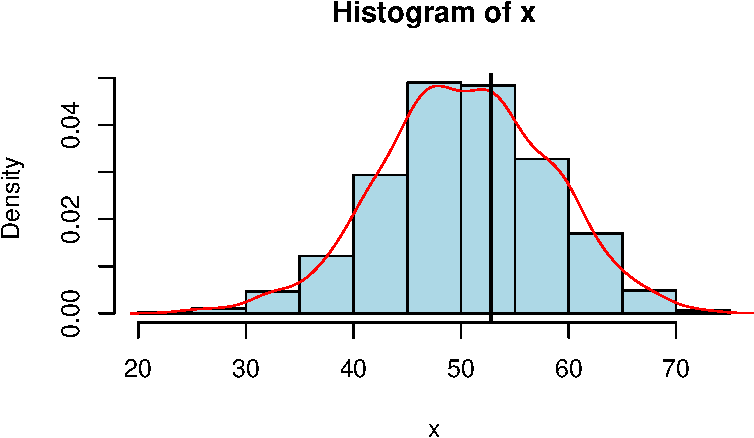
\includegraphics[keepaspectratio]{Lecture-11-Describing-a-Distribution_files/figure-pdf/unnamed-chunk-13-1.pdf}}

\subsection{Quartiles}\label{quartiles}

We have already talked some about the median and quartiles. We could
calculate the \(p^{\text{th}}\) quantile which is the value where
\(100\cdot p%
\) of the data is less than the value. This also means that
\(100\cdot (1-p)%
\) of the data is more than this value. If we are in the
\(90^\text{th}\) percentile for intelligence then we are really smart
since we score better than 90\% of people. But, if we are in the
\(17^\text{th}\) percentile for salary then we know we are only making
more money than 17\% of people (and we should probably ask for a raise).

In order to calculate different quantiles in R, we could use the
`\(quantile()\)' function. We need to pass a vector into it and tell it
where we want to set the breaks (as decimals). We can do this using the
sequence function. Below is an example of how we could do it with
quartiles and quintiles:

\begin{Shaded}
\begin{Highlighting}[]
\FunctionTok{seq}\NormalTok{(}\AttributeTok{from=}\DecValTok{0}\NormalTok{,}\AttributeTok{to=}\DecValTok{1}\NormalTok{,}\AttributeTok{by=}\FloatTok{0.25}\NormalTok{)}
\end{Highlighting}
\end{Shaded}

\begin{verbatim}
[1] 0.00 0.25 0.50 0.75 1.00
\end{verbatim}

\begin{Shaded}
\begin{Highlighting}[]
\FunctionTok{quantile}\NormalTok{(mtcars}\SpecialCharTok{$}\NormalTok{mpg, }\FunctionTok{seq}\NormalTok{(}\AttributeTok{from=}\DecValTok{0}\NormalTok{,}\AttributeTok{to=}\DecValTok{1}\NormalTok{,}\AttributeTok{by=}\FloatTok{0.25}\NormalTok{))}
\end{Highlighting}
\end{Shaded}

\begin{verbatim}
    0%    25%    50%    75%   100% 
10.400 15.425 19.200 22.800 33.900 
\end{verbatim}

\begin{Shaded}
\begin{Highlighting}[]
\FunctionTok{seq}\NormalTok{(}\AttributeTok{from=}\DecValTok{0}\NormalTok{,}\AttributeTok{to=}\DecValTok{1}\NormalTok{,}\AttributeTok{by=}\FloatTok{0.2}\NormalTok{)}
\end{Highlighting}
\end{Shaded}

\begin{verbatim}
[1] 0.0 0.2 0.4 0.6 0.8 1.0
\end{verbatim}

\subsection{Summarizing the Center and
Position}\label{summarizing-the-center-and-position}

Similar to the mode function we created earlier, we could create
functions in R to put all of the information in a single place for us.
Be careful though, as passing continuous data into it may result in
everything being outputted as a mode (you can always remove the MODE
function if you are dealing with continuous data):

\begin{Shaded}
\begin{Highlighting}[]
\NormalTok{center\_stats }\OtherTok{\textless{}{-}} \ControlFlowTok{function}\NormalTok{(x)\{}
    \FunctionTok{c}\NormalTok{(}\AttributeTok{mean=}\FunctionTok{round}\NormalTok{(}\FunctionTok{mean}\NormalTok{(x,}\AttributeTok{na.rm=}\ConstantTok{TRUE}\NormalTok{),}\DecValTok{2}\NormalTok{),}
         \AttributeTok{median=}\FunctionTok{round}\NormalTok{(}\FunctionTok{median}\NormalTok{(x,}\AttributeTok{na.rm=}\ConstantTok{TRUE}\NormalTok{),}\DecValTok{2}\NormalTok{),}
         \AttributeTok{trim25=}\FunctionTok{round}\NormalTok{(}\FunctionTok{mean}\NormalTok{(x,}\AttributeTok{trim=}\NormalTok{.}\DecValTok{25}\NormalTok{,}\AttributeTok{na.rm=}\ConstantTok{TRUE}\NormalTok{),}\DecValTok{2}\NormalTok{),}
         \AttributeTok{trim10=}\FunctionTok{round}\NormalTok{(}\FunctionTok{mean}\NormalTok{(x,}\AttributeTok{trim=}\NormalTok{.}\DecValTok{10}\NormalTok{,}\AttributeTok{na.rm=}\ConstantTok{TRUE}\NormalTok{),}\DecValTok{2}\NormalTok{),}
         \AttributeTok{mode=}\FunctionTok{round}\NormalTok{(}\FunctionTok{MODE}\NormalTok{(x),}\DecValTok{2}\NormalTok{),}
         \AttributeTok{est\_mode=}\FunctionTok{round}\NormalTok{(}\FunctionTok{estimate\_mode}\NormalTok{(x),}\DecValTok{2}\NormalTok{)}
\NormalTok{      )}
\NormalTok{\}}

\FunctionTok{center\_stats}\NormalTok{(iris}\SpecialCharTok{$}\NormalTok{Sepal.Length)}
\end{Highlighting}
\end{Shaded}

\begin{verbatim}
    mean   median   trim25   trim10     mode est_mode 
    5.84     5.80     5.80     5.81     5.00     5.72 
\end{verbatim}

\begin{Shaded}
\begin{Highlighting}[]
\FunctionTok{center\_stats}\NormalTok{(airquality}\SpecialCharTok{$}\NormalTok{Ozone)}
\end{Highlighting}
\end{Shaded}

\begin{verbatim}
    mean   median   trim25   trim10     mode est_mode 
   42.13    31.50    33.40    37.80    23.00    20.61 
\end{verbatim}

We could do something similar with our position summary as well and view
the quartiles and quantiles:

\begin{Shaded}
\begin{Highlighting}[]
\NormalTok{position\_stats }\OtherTok{\textless{}{-}} \ControlFlowTok{function}\NormalTok{(x) \{}
     \FunctionTok{list}\NormalTok{(}\AttributeTok{quint=}\FunctionTok{quantile}\NormalTok{(x,}\FunctionTok{seq}\NormalTok{(}\DecValTok{0}\NormalTok{,}\DecValTok{1}\NormalTok{,.}\DecValTok{2}\NormalTok{), }\AttributeTok{na.rm=}\ConstantTok{TRUE}\NormalTok{),}
          \AttributeTok{quart=}\FunctionTok{quantile}\NormalTok{(x,}\FunctionTok{seq}\NormalTok{(}\DecValTok{0}\NormalTok{,}\DecValTok{1}\NormalTok{,.}\DecValTok{25}\NormalTok{), }\AttributeTok{na.rm=}\ConstantTok{TRUE}\NormalTok{))}
\NormalTok{\}}

\FunctionTok{position\_stats}\NormalTok{(iris}\SpecialCharTok{$}\NormalTok{Sepal.Length)}
\end{Highlighting}
\end{Shaded}

\begin{verbatim}
$quint
  0%  20%  40%  60%  80% 100% 
4.30 5.00 5.60 6.10 6.52 7.90 

$quart
  0%  25%  50%  75% 100% 
 4.3  5.1  5.8  6.4  7.9 
\end{verbatim}

These center stats and position stats might indicate to use the the
Sepal Length of an iris is symmetric since the mean and median are
roughly the same, with no real differences in the mean and trimmed mean.
Additionally, the position stats do not show too much reason to be
concerned as the distance between the 25th and 50th percentile is
roughly the same as the distance between the 50th and 75th percentile.
We can make the same argument for the bottom half of the data and the
top half of the data and get similar results. We will see in future
sections how we can quantify the symmetry of the dataset using a
formula/number.

The last example we will look at in this section are the calculations
for the Ozone variable in the ``airquality'' dataset. The center stats
were carried out above and it indicates that this variable is not
symmetric since the mean and median are far apart along with the mean
and trimmed mean being different. Interpreting the position stats for
the variable give us similar results. We can see that the top half of
the dataset is much more spread out then the bottom half of the dataset,
indicating that we probably have a skewed distribution.

\begin{Shaded}
\begin{Highlighting}[]
\FunctionTok{position\_stats}\NormalTok{(airquality}\SpecialCharTok{$}\NormalTok{Ozone)}
\end{Highlighting}
\end{Shaded}

\begin{verbatim}
$quint
  0%  20%  40%  60%  80% 100% 
   1   14   23   39   73  168 

$quart
    0%    25%    50%    75%   100% 
  1.00  18.00  31.50  63.25 168.00 
\end{verbatim}

It is important to note that these outputs will not definitively prove
if the distribution is symmetric or not. We will need to utilize all of
the information we learn over the next few lectures along with a
visualization to make any determination. Because we will be utilizing
these functions that we have created throughout the rest of the course,
I encourage you to save them somewhere so that you can run them when
needed (like when you start a new session in R or if you need to use the
functions in an RMarkdown document).

\section{Spread Statistics}\label{spread-statistics}

There are a few descriptive statistics that we should look at in order
to gain more information about our data. The three big ones are the
center of the data, the spread of the data, and the skewness of the
data. We have already seen how central tendency can tell us about a
dataset in terms of the symmetry of the data. In this lecture, we will
look into what the spread of the data can tell and relate some of this
information back to the idea of symmetry.

Let's assume that we are given two different sets of data regarding
salaries at two different companies. If I told you that employees at
both companies earned an average of \$75,000 then might consider both
sets of data to be about the same. This is not quite true though, as
every employee at Company A could make exactly \$75,000 while most
employees at Company B make \$50,000 with a single outlier (probably the
CEO) making a ton of money, thus bringing the mean to \$75,000. This
example should show us that the central tendency of a dataset by itself
does not tell us the whole picture, we also need to provide the spread
of the data. There are a few different ways that we can describe the
spread of our data; the two simplest methods would be using our Range
Difference and our Standard Deviation (two methods we have already
discussed).

\subsection{Variance}\label{variance}

One way to describe the range of a dataset is to calculate the variance
of the data. This will tell us how far (on average) data varies from the
mean. This should sound extremely similar to our standard deviation,
which is expected since the two are related. In fact, the variance
(\(\sigma^2\)) is the standard deviation (\(\sigma\)) squared. Its exact
formula can be seen below:
\[ \text{variance } = \sigma^2 = \frac{\sum_{i=1}^n (x_1-\bar{x})^2}{n-1}\]

It should be noted that the units are squared for variance. This means
that if our data is measuring pounds then the variance will be in
pounds\(^2\). Taking the square root of the variance will give us the
standard deviation. The idea of variance and standard deviation allows
us to compare two sets of data that have the same units. Below, we can
see the calculation in R using a formula and the built-in function and
how it relates to standard deviation:

\begin{Shaded}
\begin{Highlighting}[]
\NormalTok{x }\OtherTok{\textless{}{-}} \FunctionTok{c}\NormalTok{(}\DecValTok{4}\NormalTok{, }\DecValTok{7}\NormalTok{, }\DecValTok{3}\NormalTok{, }\DecValTok{1}\NormalTok{, }\DecValTok{7}\NormalTok{, }\DecValTok{9}\NormalTok{, }\DecValTok{5}\NormalTok{, }\DecValTok{3}\NormalTok{, }\DecValTok{2}\NormalTok{, }\DecValTok{6}\NormalTok{, }\DecValTok{8}\NormalTok{)}
\FunctionTok{sum}\NormalTok{((x}\SpecialCharTok{{-}}\FunctionTok{mean}\NormalTok{(x))}\SpecialCharTok{\^{}}\DecValTok{2}\NormalTok{)}\SpecialCharTok{/}\NormalTok{(}\FunctionTok{length}\NormalTok{(x)}\SpecialCharTok{{-}}\DecValTok{1}\NormalTok{) }\CommentTok{\# Variance}
\end{Highlighting}
\end{Shaded}

\begin{verbatim}
[1] 6.8
\end{verbatim}

\begin{Shaded}
\begin{Highlighting}[]
\FunctionTok{var}\NormalTok{(x)}
\end{Highlighting}
\end{Shaded}

\begin{verbatim}
[1] 6.8
\end{verbatim}

\begin{Shaded}
\begin{Highlighting}[]
\FunctionTok{sqrt}\NormalTok{(}\FloatTok{6.8}\NormalTok{) }\CommentTok{\# Standard Deviation}
\end{Highlighting}
\end{Shaded}

\begin{verbatim}
[1] 2.607681
\end{verbatim}

\begin{Shaded}
\begin{Highlighting}[]
\FunctionTok{sd}\NormalTok{(x)}
\end{Highlighting}
\end{Shaded}

\begin{verbatim}
[1] 2.607681
\end{verbatim}

If we go back to our previous example about salary, we can compare the
two groups using both the mean and the standard deviation. If we found
the standard deviation of Company A to be \$5,000 and Company B to be
\$30,000 then we could say that the salaries at Company B are much more
spread out than at Company A. The mean and the standard deviation should
always be interpreted together, as just knowing one does not tell us the
full picture of the data.

\begin{watch}{}{}
    \href{https://youtu.be/8_7Qht9poF0}{Describing the Spread of Data using Variance}
\end{watch}

\subsection{Inter-Quartile Range (IQR)}\label{inter-quartile-range-iqr}

Another way that we can describe the spread of the data is through
quartiles. We touched on quartiles in the previous section and mentioned
that they break up the data into ``quarters''. In order to calculate the
different quartile values (First Quartile=Q1, Second Quartile=Median=Q2,
and Third Quartile=Q3) we will first need to order our data from
smallest to largest and then identify the middle value. This middle
value of the dataset will be the median, also known as Q2. This tells us
the value such that 50\% of the data is below it and 50\% of the data is
above it.

Once we have found the median, we can break our data up into a ``lower''
half and an ``upper'' half. We then find the median of each of those
groups and that tells us what our Q1 and Q3 are. The First Quartile (Q1)
will tell us the value such that 25\% of the data is below it (and thus
75\% of the data is above it). Likewise, the Third Quartile (Q3) will
tell us the value such that 75\% of the data is below is (and thus 25\%
of the data is above it). An example of this can be seen in the dataset
below:

\begin{center}
\pandocbounded{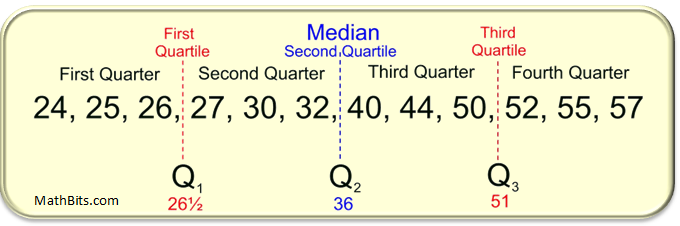
\includegraphics[keepaspectratio]{images/L11-Quartiles.png}}
\end{center}

It should probably be mentioned that R sometimes calculates quartiles a
little bit differently than you may expect. That is because there are
actually nine(!) different ways programmed in R. We can choose different
methods using the `type=' argument in our `quantile()' function. Below
is an example of carrying out the process in R and seeing that we get
different results than the picture above depending on the type we select
to caclulate the quartiles. Don't worry about the small differences or
the details as all of the results will give us similar values, and it
will not affect any calculations we do. I just wanted to point this out
in case we try finding it by hand or use an online calculator and then
compare it to R and notice that it is different.

\begin{Shaded}
\begin{Highlighting}[]
\NormalTok{x }\OtherTok{\textless{}{-}} \FunctionTok{c}\NormalTok{(}\DecValTok{24}\NormalTok{, }\DecValTok{25}\NormalTok{, }\DecValTok{26}\NormalTok{, }\DecValTok{27}\NormalTok{, }\DecValTok{30}\NormalTok{, }\DecValTok{32}\NormalTok{, }\DecValTok{40}\NormalTok{, }\DecValTok{44}\NormalTok{, }\DecValTok{50}\NormalTok{, }\DecValTok{52}\NormalTok{, }\DecValTok{55}\NormalTok{, }\DecValTok{57}\NormalTok{)}
\FunctionTok{summary}\NormalTok{(x)}
\end{Highlighting}
\end{Shaded}

\begin{verbatim}
   Min. 1st Qu.  Median    Mean 3rd Qu.    Max. 
  24.00   26.75   36.00   38.50   50.50   57.00 
\end{verbatim}

\begin{Shaded}
\begin{Highlighting}[]
\FunctionTok{quantile}\NormalTok{(x, }\FunctionTok{c}\NormalTok{(}\DecValTok{0}\NormalTok{,.}\DecValTok{25}\NormalTok{,.}\DecValTok{50}\NormalTok{,.}\DecValTok{75}\NormalTok{,}\DecValTok{1}\NormalTok{))}
\end{Highlighting}
\end{Shaded}

\begin{verbatim}
   0%   25%   50%   75%  100% 
24.00 26.75 36.00 50.50 57.00 
\end{verbatim}

\begin{Shaded}
\begin{Highlighting}[]
\FunctionTok{quantile}\NormalTok{(x, }\FunctionTok{c}\NormalTok{(}\DecValTok{0}\NormalTok{,.}\DecValTok{25}\NormalTok{,.}\DecValTok{50}\NormalTok{,.}\DecValTok{75}\NormalTok{,}\DecValTok{1}\NormalTok{), }\AttributeTok{type=}\DecValTok{5}\NormalTok{)}
\end{Highlighting}
\end{Shaded}

\begin{verbatim}
  0%  25%  50%  75% 100% 
24.0 26.5 36.0 51.0 57.0 
\end{verbatim}

\begin{Shaded}
\begin{Highlighting}[]
\FunctionTok{quantile}\NormalTok{(x, }\FunctionTok{c}\NormalTok{(}\DecValTok{0}\NormalTok{,.}\DecValTok{25}\NormalTok{,.}\DecValTok{50}\NormalTok{,.}\DecValTok{75}\NormalTok{,}\DecValTok{1}\NormalTok{), }\AttributeTok{type=}\DecValTok{6}\NormalTok{)}
\end{Highlighting}
\end{Shaded}

\begin{verbatim}
   0%   25%   50%   75%  100% 
24.00 26.25 36.00 51.50 57.00 
\end{verbatim}

We can use these quartiles to determine the spread of our data along
with if the data is possibly symmetric. Remember that when we do this
``Quartile Analysis'', we want to check that the Median-Minimum is
roughly the same size as the Maximum-Median. Additionally, we want to
check whether Q1-Minimum is roughly similar to Maximum-Q3 and if
Median-Q1 is roughly similar to Q3-Median. Going through this process,
we may see that data on one side of the median is more spread out, which
may indicate the data is skewed toward that side.

We can go a little bit further and introduce the idea of the
Inter-Quartile Range (IQR). This will be calculated as the middle 50\%
of the data (or Q3-Q1). This is important as it tells us how spread out
the middle part of our data is. Typically, it is said that data below
\(Q1-1.5\cdot IQR\) or above \(Q3+1.5\cdot IQR\) are considered
outliers.

\begin{center}
\pandocbounded{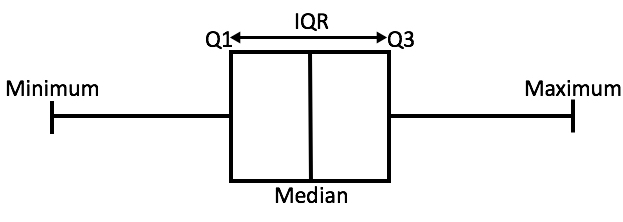
\includegraphics[keepaspectratio]{images/L11-IQR.png}}
\end{center}

We can calculate the Inter-Quartile Range, as well as our other quartile
ranges used in our ``Quartile Analysis'' using the quantile function in
R. We can see that the two halves are not the same ``size'', indicating
potential positive skew due to the ``right side'' being bigger then the
``left side''.

\begin{Shaded}
\begin{Highlighting}[]
\FunctionTok{median}\NormalTok{(mtcars}\SpecialCharTok{$}\NormalTok{mpg) }\SpecialCharTok{{-}} \FunctionTok{min}\NormalTok{(mtcars}\SpecialCharTok{$}\NormalTok{mpg)}
\end{Highlighting}
\end{Shaded}

\begin{verbatim}
[1] 8.8
\end{verbatim}

\begin{Shaded}
\begin{Highlighting}[]
\FunctionTok{max}\NormalTok{(mtcars}\SpecialCharTok{$}\NormalTok{mpg) }\SpecialCharTok{{-}} \FunctionTok{median}\NormalTok{(mtcars}\SpecialCharTok{$}\NormalTok{mpg)}
\end{Highlighting}
\end{Shaded}

\begin{verbatim}
[1] 14.7
\end{verbatim}

Looking at the different Quartile Ranges we can see that the middle
sections are fairly symmetric, which indicates that the tails may be the
thing causing the skew to occur.

\begin{Shaded}
\begin{Highlighting}[]
\FunctionTok{median}\NormalTok{(mtcars}\SpecialCharTok{$}\NormalTok{mpg) }\SpecialCharTok{{-}} \FunctionTok{quantile}\NormalTok{(mtcars}\SpecialCharTok{$}\NormalTok{mpg, .}\DecValTok{25}\NormalTok{)}
\end{Highlighting}
\end{Shaded}

\begin{verbatim}
  25% 
3.775 
\end{verbatim}

\begin{Shaded}
\begin{Highlighting}[]
\FunctionTok{quantile}\NormalTok{(mtcars}\SpecialCharTok{$}\NormalTok{mpg, .}\DecValTok{75}\NormalTok{) }\SpecialCharTok{{-}} \FunctionTok{median}\NormalTok{(mtcars}\SpecialCharTok{$}\NormalTok{mpg)}
\end{Highlighting}
\end{Shaded}

\begin{verbatim}
75% 
3.6 
\end{verbatim}

\begin{Shaded}
\begin{Highlighting}[]
\CommentTok{\# We have a symmetric middle since values are about the same}
\end{Highlighting}
\end{Shaded}

We can also calculate our IQR in R and we can see that 50\% of our data
only falls over a range of roughly 7.4 mpg.

\begin{Shaded}
\begin{Highlighting}[]
\FunctionTok{quantile}\NormalTok{(mtcars}\SpecialCharTok{$}\NormalTok{mpg, .}\DecValTok{75}\NormalTok{) }\SpecialCharTok{{-}} \FunctionTok{quantile}\NormalTok{(mtcars}\SpecialCharTok{$}\NormalTok{mpg, .}\DecValTok{25}\NormalTok{) }\CommentTok{\# This is our IQR}
\end{Highlighting}
\end{Shaded}

\begin{verbatim}
  75% 
7.375 
\end{verbatim}

Finally, looking at our quartile ranges for the tails we can see that
the skewness is on the right side due to the upper 25\% of the data
taking up more room than the lower 25\% of the data.

\begin{Shaded}
\begin{Highlighting}[]
\FunctionTok{quantile}\NormalTok{(mtcars}\SpecialCharTok{$}\NormalTok{mpg, .}\DecValTok{25}\NormalTok{) }\SpecialCharTok{{-}} \FunctionTok{min}\NormalTok{(mtcars}\SpecialCharTok{$}\NormalTok{mpg)}
\end{Highlighting}
\end{Shaded}

\begin{verbatim}
  25% 
5.025 
\end{verbatim}

\begin{Shaded}
\begin{Highlighting}[]
\FunctionTok{max}\NormalTok{(mtcars}\SpecialCharTok{$}\NormalTok{mpg)}\SpecialCharTok{{-}}\FunctionTok{quantile}\NormalTok{(mtcars}\SpecialCharTok{$}\NormalTok{mpg,.}\DecValTok{75}\NormalTok{)}
\end{Highlighting}
\end{Shaded}

\begin{verbatim}
 75% 
11.1 
\end{verbatim}

\begin{Shaded}
\begin{Highlighting}[]
\CommentTok{\# May indicate a positive skew since right{-}half is bigger than left{-}half}
\end{Highlighting}
\end{Shaded}

\begin{watch}{}{}
    \href{https://youtu.be/5GPioBqp2Og}{Discussing Quartiles and the Inter-Quartile Range}
\end{watch}

\subsection{Z-Score (Normalization)}\label{z-score-normalization}

If we wish to compare two sets of data, then we can Normalize the data.
What we are doing here is centering our data around the mean and then
dividing it by the standard deviation in order for us to have a unitless
value. Doing this will allow us to compare sets with either the same or
different units. It also allows us to not have to define what a ``big''
difference or a ``big'' range is like we did before to identify the
skew. It makes all of the data normalized and thus easier to read and
compare with differing groups. We have seen this idea before with the
idea of the \(z\)-score, which tells us how many standard deviations
above (or below) the mean a value is:

\[ z\text{-score} = \frac{\text{value} - \text{mean}}{\text{standard deviation}}\]

This idea of normalization often allows us to apply the z-score
technique to Normal Distributions. This will give us the Standard Normal
Distribution with a mean of 0 and a standard deviation of 1, denoted as
N(0,1). If we were to plot a standard normal distribution, it would look
like the figure below, with a z-score of 1 indicating a value of 1
standard deviation above the mean and a z-score of -2 indicating a value
of 2 standard deviations below the mean.

\begin{center}
\pandocbounded{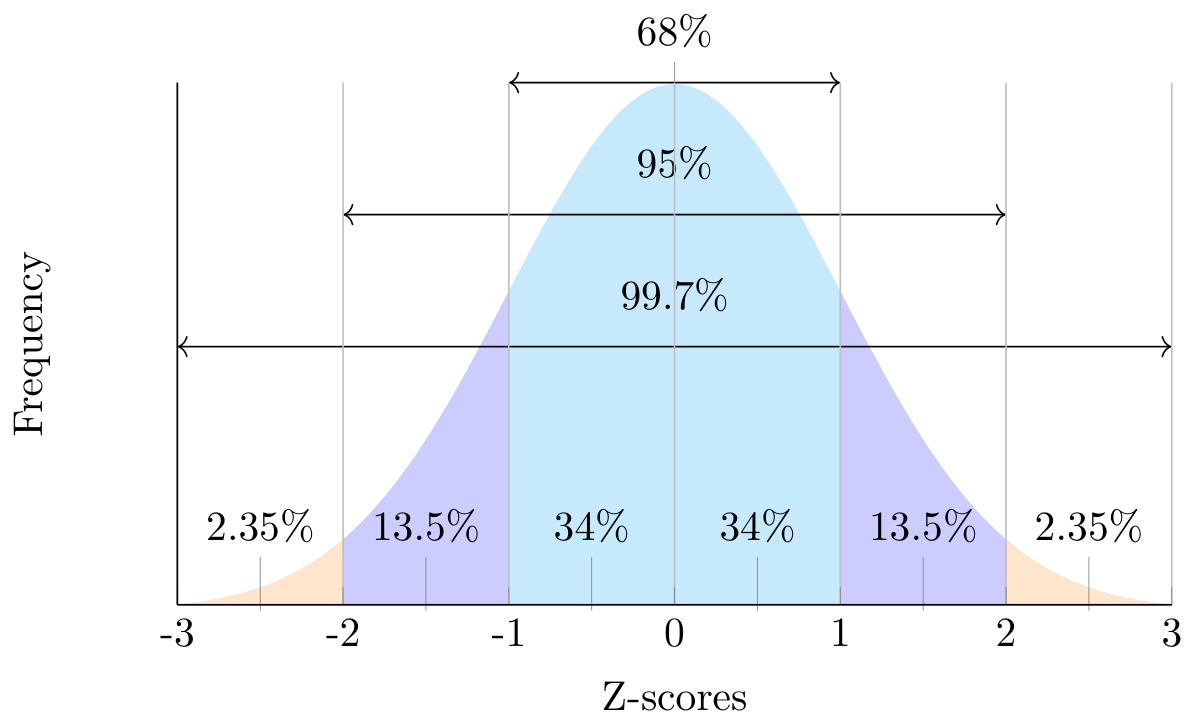
\includegraphics[keepaspectratio]{images/L11-Normal-Distribution.png}}
\end{center}

Note that the idea of normalized data can be carried out on any set of
data as well as descriptive statistics, allowing us to indicate the skew
of the data. Below is an example of standardizing the data in R making
it easier to see the right-skew:

\begin{Shaded}
\begin{Highlighting}[]
\FunctionTok{summary}\NormalTok{( (mtcars}\SpecialCharTok{$}\NormalTok{mpg}\SpecialCharTok{{-}}\FunctionTok{mean}\NormalTok{(mtcars}\SpecialCharTok{$}\NormalTok{mpg))}\SpecialCharTok{/}\FunctionTok{sd}\NormalTok{(mtcars}\SpecialCharTok{$}\NormalTok{mpg) )}
\end{Highlighting}
\end{Shaded}

\begin{verbatim}
   Min. 1st Qu.  Median    Mean 3rd Qu.    Max. 
-1.6079 -0.7741 -0.1478  0.0000  0.4495  2.2913 
\end{verbatim}

We could also compare the percentages within 1, 2, and 3 standard
deviations if we were to write a function. It will allow us to learn
about where the data lies as well as the thickness of the tails, which
we will discuss in the next section. Once again, we do not need to
understand how to write a function in R, we just need to know the
general idea of what it is doing.

\begin{Shaded}
\begin{Highlighting}[]
\NormalTok{pct }\OtherTok{\textless{}{-}} \ControlFlowTok{function}\NormalTok{(x,n) \{}
\NormalTok{     lbnd }\OtherTok{\textless{}{-}} \FunctionTok{mean}\NormalTok{(x,}\AttributeTok{na.rm=}\ConstantTok{TRUE}\NormalTok{) }\SpecialCharTok{{-}}\NormalTok{ n}\SpecialCharTok{*}\FunctionTok{sd}\NormalTok{(x,}\AttributeTok{na.rm=}\ConstantTok{TRUE}\NormalTok{)}
\NormalTok{     ubnd }\OtherTok{\textless{}{-}} \FunctionTok{mean}\NormalTok{(x,}\AttributeTok{na.rm=}\ConstantTok{TRUE}\NormalTok{) }\SpecialCharTok{+}\NormalTok{ n}\SpecialCharTok{*}\FunctionTok{sd}\NormalTok{(x,}\AttributeTok{na.rm=}\ConstantTok{TRUE}\NormalTok{)}
\NormalTok{     (pct }\OtherTok{\textless{}{-}} \FunctionTok{round}\NormalTok{(}\FunctionTok{length}\NormalTok{(x[x}\SpecialCharTok{\textgreater{}=}\NormalTok{lbnd }\SpecialCharTok{\&}\NormalTok{ x}\SpecialCharTok{\textless{}=}\NormalTok{ubnd])}\SpecialCharTok{/}\FunctionTok{length}\NormalTok{(x)}\SpecialCharTok{*}\DecValTok{100}\NormalTok{,}\DecValTok{2}\NormalTok{))}
\NormalTok{\}}
\end{Highlighting}
\end{Shaded}

We can use this function to see what percent of the data is within 1, 2,
and 3 standard deviations. We know that a normal distribution will
roughly follow the 68-95-99.7 rule in terms of the spread of the data.
If I were to do this in R I could get the following results:

\begin{Shaded}
\begin{Highlighting}[]
\FunctionTok{pct}\NormalTok{(mtcars}\SpecialCharTok{$}\NormalTok{mpg, }\DecValTok{1}\NormalTok{) }\CommentTok{\# Expecting 68}
\end{Highlighting}
\end{Shaded}

\begin{verbatim}
[1] 75
\end{verbatim}

\begin{Shaded}
\begin{Highlighting}[]
\FunctionTok{pct}\NormalTok{(mtcars}\SpecialCharTok{$}\NormalTok{mpg, }\DecValTok{2}\NormalTok{) }\CommentTok{\# Expecting 95}
\end{Highlighting}
\end{Shaded}

\begin{verbatim}
[1] 93.75
\end{verbatim}

\begin{Shaded}
\begin{Highlighting}[]
\FunctionTok{pct}\NormalTok{(mtcars}\SpecialCharTok{$}\NormalTok{mpg, }\DecValTok{3}\NormalTok{) }\CommentTok{\# Expecting 99.7}
\end{Highlighting}
\end{Shaded}

\begin{verbatim}
[1] 100
\end{verbatim}

The results above indicate that we have more data within 1 and 3
standard deviations than we would expect. This may indicate skewness in
our data along with a different tail thickness than a normal
distribution (but that will come next time)

\begin{watch}{}{}
    \href{https://youtu.be/9ckiM6PbICI}{Normalizing the Data and using the \textit{pct()} function}
\end{watch}

\subsection{Summarizing the Spread using
Functions}\label{summarizing-the-spread-using-functions}

We could build a function to help us summarize the spread of our data.
This function will calculate the standard deviation, IQR, the normalized
minimum, maximum, and range as well as the percentage of data within 1,
2, and 3 standard deviations:

\begin{Shaded}
\begin{Highlighting}[]
\NormalTok{spread\_stats }\OtherTok{\textless{}{-}} \ControlFlowTok{function}\NormalTok{(x)\{}
    \FunctionTok{c}\NormalTok{(}\AttributeTok{sd=}\FunctionTok{round}\NormalTok{(}\FunctionTok{sd}\NormalTok{(x,}\AttributeTok{na.rm=}\ConstantTok{TRUE}\NormalTok{),}\DecValTok{2}\NormalTok{),}
    \AttributeTok{iqr=}\FunctionTok{round}\NormalTok{(}\FunctionTok{IQR}\NormalTok{(x,}\AttributeTok{na.rm=}\ConstantTok{TRUE}\NormalTok{),}\DecValTok{2}\NormalTok{),}
    \AttributeTok{minz=}\FunctionTok{round}\NormalTok{(}\FunctionTok{range}\NormalTok{(}\FunctionTok{scale}\NormalTok{(x),}\AttributeTok{na.rm=}\ConstantTok{TRUE}\NormalTok{)[}\DecValTok{1}\NormalTok{],}\DecValTok{2}\NormalTok{),}
    \AttributeTok{maxz=}\FunctionTok{round}\NormalTok{(}\FunctionTok{range}\NormalTok{(}\FunctionTok{scale}\NormalTok{(x),}\AttributeTok{na.rm=}\ConstantTok{TRUE}\NormalTok{)[}\DecValTok{2}\NormalTok{],}\DecValTok{2}\NormalTok{),}
    \AttributeTok{diffz=}\FunctionTok{round}\NormalTok{(}\FunctionTok{diff}\NormalTok{(}\FunctionTok{range}\NormalTok{(}\FunctionTok{scale}\NormalTok{(x),}\AttributeTok{na.rm=}\ConstantTok{TRUE}\NormalTok{)),}\DecValTok{2}\NormalTok{),}
    \AttributeTok{prp1=}\FunctionTok{round}\NormalTok{(}\FunctionTok{pct}\NormalTok{(x,}\DecValTok{1}\NormalTok{),}\DecValTok{2}\NormalTok{),}
    \AttributeTok{prp2=}\FunctionTok{round}\NormalTok{(}\FunctionTok{pct}\NormalTok{(x,}\DecValTok{2}\NormalTok{),}\DecValTok{2}\NormalTok{),}
    \AttributeTok{prp3=}\FunctionTok{round}\NormalTok{(}\FunctionTok{pct}\NormalTok{(x,}\DecValTok{3}\NormalTok{),}\DecValTok{2}\NormalTok{))}
\NormalTok{\}}
\FunctionTok{spread\_stats}\NormalTok{(mtcars}\SpecialCharTok{$}\NormalTok{mpg)}
\end{Highlighting}
\end{Shaded}

\begin{verbatim}
    sd    iqr   minz   maxz  diffz   prp1   prp2   prp3 
  6.03   7.38  -1.61   2.29   3.90  75.00  93.75 100.00 
\end{verbatim}

\begin{watch}{}{}
    \href{https://youtu.be/6WKsAQJTPTE}{Summarizing the data using the \textit{spread\_stats()} function}
\end{watch}

\section{Skew Statistics}\label{skew-statistics}

So far we have discussed what the center and the spread of the data can
tell us about symmetry. Remember that for data to be symmetric the mean
has to equal the median. In this lecture, we will look into how we can
measure the shape of the distribution using symmetry, skewness, and the
tails of the data.

\subsection{Skewness}\label{skewness}

We have seen that extreme values have the potential to impact the mean.
This can cause the data to be skewed to either the right side or to the
left side. Extreme values above the mean make the tail longer on the
right while extreme values below the mean make the tail longer on the
left. We can quantify skew using the following formula:

\[ \text{skew}=\frac{\frac{1}{n}\sum_{i=1}^n (x_i - \bar{x})^3}{s^3} = \frac{1}{n} \sum_{i=1}^n z_i^3 \]

If the value of the skew is positive then the data will be right-skewed
and if the skew is negative then it will be left-skewed. A skew of 0
will indicate that we may have a symmetric distribution. Values between
-0.5 and 0.5 can probably be considered fairly symmetric. If the skew
lies between -0.5 and -1 or 0.5 and 1 then we can consider it moderately
skewed, and values more extreme will be considered highly skewed. We
have a formula in R that we can implement to calculate the skew for us:

\begin{Shaded}
\begin{Highlighting}[]
\NormalTok{skew }\OtherTok{\textless{}{-}} \ControlFlowTok{function}\NormalTok{(x) \{}
\NormalTok{            z }\OtherTok{\textless{}{-}}\NormalTok{ (x}\SpecialCharTok{{-}}\FunctionTok{mean}\NormalTok{(x,}\AttributeTok{na.rm=}\ConstantTok{TRUE}\NormalTok{))}\SpecialCharTok{/}\FunctionTok{sd}\NormalTok{(x,}\AttributeTok{na.rm=}\ConstantTok{TRUE}\NormalTok{)}
            \FunctionTok{mean}\NormalTok{(z}\SpecialCharTok{\^{}}\DecValTok{3}\NormalTok{,}\AttributeTok{na.rm=}\ConstantTok{TRUE}\NormalTok{)}
\NormalTok{\}}
\end{Highlighting}
\end{Shaded}

We can test this function out on data we have shown to be both skewed
and symmetric:

\begin{Shaded}
\begin{Highlighting}[]
\FunctionTok{skew}\NormalTok{(}\FunctionTok{rgamma}\NormalTok{(}\DecValTok{500}\NormalTok{,}\DecValTok{2}\NormalTok{,}\AttributeTok{scale=}\DecValTok{5}\NormalTok{)) }\CommentTok{\# Have shown this to be skewed}
\end{Highlighting}
\end{Shaded}

\begin{verbatim}
[1] 1.235291
\end{verbatim}

\begin{Shaded}
\begin{Highlighting}[]
\FunctionTok{skew}\NormalTok{(}\FunctionTok{rnorm}\NormalTok{(}\DecValTok{500}\NormalTok{,}\DecValTok{0}\NormalTok{,}\DecValTok{2}\NormalTok{)) }\CommentTok{\# Have shown this to be symmetric}
\end{Highlighting}
\end{Shaded}

\begin{verbatim}
[1] 0.03632744
\end{verbatim}

\begin{Shaded}
\begin{Highlighting}[]
\FunctionTok{skew}\NormalTok{(mtcars}\SpecialCharTok{$}\NormalTok{mpg) }\CommentTok{\# Have shown this to be moderately skewed}
\end{Highlighting}
\end{Shaded}

\begin{verbatim}
[1] 0.610655
\end{verbatim}

These values should validate the calculations we did earlier relating to
center and spread. We still want to go through the process of our
``Quartile Analysis'' and other steps to verify that we are skewed, as
we do not want to just rely on the visualization (though it can help
confirm) to determine symmetry/skew.

If we do happen to have extreme values or highly skewed data then we
will probably not want to use the mean and standard deviation. This is
because these statistics are highly influenced by outliers. Instead, we
will want to consider using the Median and IQR to give better measures
of the center and spread of the data.

\begin{watch}{}{}
    \href{https://youtu.be/_VHtL0hgaKA}{Describing the Skew of the Data}
\end{watch}

\subsection{Kurtosis}\label{kurtosis}

Another important thing to look at when it comes to the shape of the
distribution is the kurtosis. This tells us information about the tails
of our data, specifically if they are thinner or thicker than the tails
of a normal distribution. If there are extreme values then data is
``pulled'' into the tails, resulting in the ``thicker tails''. If our
data has thicker tails then we will call it ``leptokurtic''. If there is
less data in the tails (meaning the tails are ``thinner'') then there is
a minimal impact of extreme values. This will be called ``platykurtic''.
We can visualize what both of these look like (with mesokurtic being
normally distributed)

\begin{center}
\pandocbounded{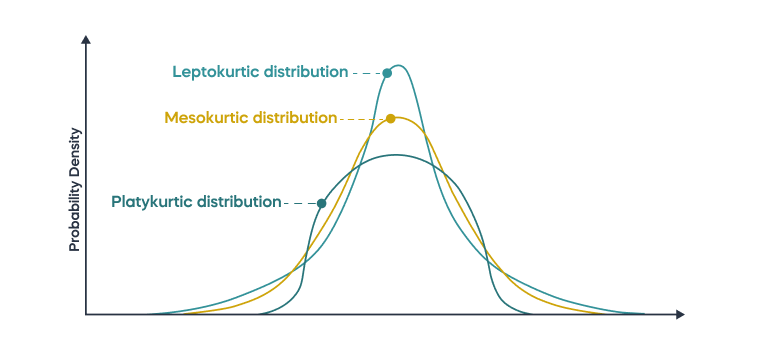
\includegraphics[keepaspectratio]{images/L11-kurtosis.png}}
\end{center}

This idea of looking at the tails is important in allowing us to compare
the data with a normal distribution. We know through the 68-95-99.7 rule
that if we have a normal distribution then roughly 68\% of the data is
within 1 standard deviation, 95\% of the data is within 2 standard
deviations, and 99.7\% of the data is within 3 standard deviations. So,
if we calculate the proportion of data within 1 standard deviation from
the mean and get a value less than 68\% then we have the potential for
thicker tails (and thus more extreme values), while a value greater than
68\% indicates that we have thinner tails (and thus fewer extreme
values).

We can also quantify the kurtosis with the formula below. If the
kurtosis is positive then we have more values in the tails (leptokurtic)
and if the kurtosis is negative then we have fewer values in the tails
than a normal distribution (platykurtic).

\[ \text{kurtosis} = \frac{1}{n} \sum_{i=1}^n z_i^4 - 3 \]

We can create a function in R that will calculate the kurtosis for us:

\begin{Shaded}
\begin{Highlighting}[]
\NormalTok{kurt }\OtherTok{\textless{}{-}} \ControlFlowTok{function}\NormalTok{(x) \{}
\NormalTok{            z }\OtherTok{\textless{}{-}}\NormalTok{ (x}\SpecialCharTok{{-}}\FunctionTok{mean}\NormalTok{(x,}\AttributeTok{na.rm=}\ConstantTok{TRUE}\NormalTok{))}\SpecialCharTok{/}\FunctionTok{sd}\NormalTok{(x,}\AttributeTok{na.rm=}\ConstantTok{TRUE}\NormalTok{)}
            \FunctionTok{mean}\NormalTok{(z}\SpecialCharTok{\^{}}\DecValTok{4}\NormalTok{,}\AttributeTok{na.rm=}\ConstantTok{TRUE}\NormalTok{) }\SpecialCharTok{{-}} \DecValTok{3}
\NormalTok{\}}
\end{Highlighting}
\end{Shaded}

We can then use this function to calculate the kurtosis for the `mpg'
vector in the `mtcars' dataset. In the previous lecture, we saw that
100\% of the data was within 3 standard deviations, implying that it has
thinner tails than a normal distribution. Therefore we would expect the
kurtosis to be negative.

\begin{Shaded}
\begin{Highlighting}[]
\FunctionTok{kurt}\NormalTok{(mtcars}\SpecialCharTok{$}\NormalTok{mpg)}
\end{Highlighting}
\end{Shaded}

\begin{verbatim}
[1] -0.372766
\end{verbatim}

We could also write a function to combine the skew and kurtosis
calculations into a single function to use. For instance, we can see in
the dataset `mlb\_teams' that the Wins column is moderately skewed left
and that it has thicker tails than the normal distribution.

\begin{Shaded}
\begin{Highlighting}[]
\NormalTok{shape\_stats }\OtherTok{\textless{}{-}} \ControlFlowTok{function}\NormalTok{(x) \{}
                    \FunctionTok{c}\NormalTok{(}\AttributeTok{skew=}\FunctionTok{round}\NormalTok{(}\FunctionTok{skew}\NormalTok{(x),}\DecValTok{2}\NormalTok{),}
                    \AttributeTok{kurt=}\FunctionTok{round}\NormalTok{(}\FunctionTok{kurt}\NormalTok{(x),}\DecValTok{2}\NormalTok{))}
\NormalTok{\}}
\end{Highlighting}
\end{Shaded}

\begin{Shaded}
\begin{Highlighting}[]
\FunctionTok{library}\NormalTok{(openintro)}
\end{Highlighting}
\end{Shaded}

\begin{Shaded}
\begin{Highlighting}[]
\FunctionTok{shape\_stats}\NormalTok{(mlb\_teams}\SpecialCharTok{$}\NormalTok{wins)}
\end{Highlighting}
\end{Shaded}

\begin{verbatim}
 skew  kurt 
-0.75  0.82 
\end{verbatim}

\begin{Shaded}
\begin{Highlighting}[]
\FunctionTok{shape\_stats}\NormalTok{(mtcars}\SpecialCharTok{$}\NormalTok{mpg)}
\end{Highlighting}
\end{Shaded}

\begin{verbatim}
 skew  kurt 
 0.61 -0.37 
\end{verbatim}

\begin{watch}{}{}
    \href{https://youtu.be/_WWocrj60bo}{Describing the Kurtosis of the Data}
\end{watch}

\subsection{Mode and Shape}\label{mode-and-shape}

The Mode of a distribution is directly related to the shape. If we have
symmetric data and it is uni-modal (one mode) then all of the values are
clustered around a single point. If data is bi-modal (two modes) then
the data is clustered around two points. We could extend this idea of
clustering to occur around multiple points. Typically, if there are
multiple modes then there are probably multiple populations included in
the dataset. This may be able to be ``broken'' apart using categorical
variables. An example of this would be the average height of students
may be bi-modal due to males and females having different average
heights.

\begin{center}
\pandocbounded{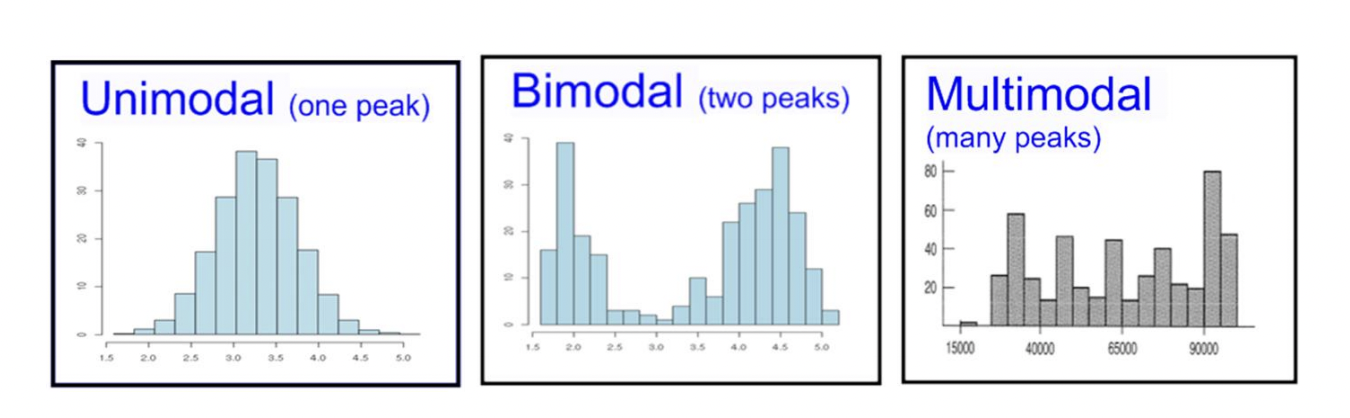
\includegraphics[keepaspectratio]{images/L11-Modals.png}}
\end{center}

\subsection{Assessing the Data}\label{assessing-the-data}

Now that we can look at the center, the spread, and the skew of the data
we can start talking about how to assess the data. We might ask
ourselves what relationships and patterns can be seen and what
transformations might help us gain a deeper understanding of the data.

Looking at the `babies' dataframe with a specific focus on the `bwt'
column, we can run through our exercises to learn about the center,
spread, and skew. We should be able to determine that this is unimodal
data which has a slight negative skew and slightly thicker tails than a
normal distribution. There is also a minimal impact from extreme values.
We can visualize this data and compare it to a normal distribution (the
red line) to see how it would compare:

\begin{Shaded}
\begin{Highlighting}[]
\FunctionTok{hist}\NormalTok{(babies}\SpecialCharTok{$}\NormalTok{bwt,}\AttributeTok{freq=}\ConstantTok{FALSE}\NormalTok{)}
\FunctionTok{lines}\NormalTok{(}\FunctionTok{density}\NormalTok{(babies}\SpecialCharTok{$}\NormalTok{bwt),}\AttributeTok{col=}\StringTok{"blue"}\NormalTok{)}
\NormalTok{xfit }\OtherTok{\textless{}{-}} \FunctionTok{seq}\NormalTok{(}\DecValTok{0}\NormalTok{,}\FunctionTok{max}\NormalTok{(babies}\SpecialCharTok{$}\NormalTok{bwt),.}\DecValTok{1}\NormalTok{)}
\NormalTok{yfit }\OtherTok{\textless{}{-}} \FunctionTok{dnorm}\NormalTok{(xfit,}\AttributeTok{mean=}\FunctionTok{mean}\NormalTok{(babies}\SpecialCharTok{$}\NormalTok{bwt), }\AttributeTok{sd=}\FunctionTok{sd}\NormalTok{(babies}\SpecialCharTok{$}\NormalTok{bwt,}\AttributeTok{na.rm=}\ConstantTok{TRUE}\NormalTok{))}
\FunctionTok{lines}\NormalTok{(xfit, yfit, }\AttributeTok{col=}\StringTok{"red"}\NormalTok{, }\AttributeTok{lwd=}\DecValTok{2}\NormalTok{)}
\end{Highlighting}
\end{Shaded}

\pandocbounded{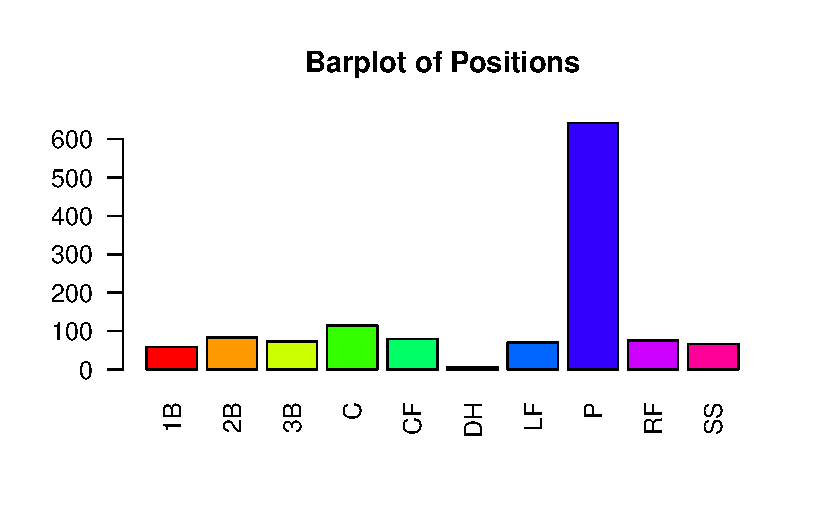
\includegraphics[keepaspectratio]{Lecture-11-Describing-a-Distribution_files/figure-pdf/unnamed-chunk-35-1.pdf}}

\begin{watch}{}{}
    \href{https://youtu.be/R20OrKJMHnc}{Putting it all together}
\end{watch}

\bookmarksetup{startatroot}

\chapter{Central Limit Theorem}\label{central-limit-theorem}

In this section, we will run through some simulations to see the Central
Limit Theorem in action. There will be a good amount of code and
outputs, but the majority of the code is virtually the same thing. You
are encouraged to run through the code yourself and play around with it
to see what each piece may do.

\section{Probability}\label{probability}

In order have have a solid grasp of statistics and data science, one
needs to understand probability. We will say that P(event), which is
read as ``the probability of an event'', tells us the likelihood of an
event occurring. For discrete data it might be a specific value and for
continuous data it may be a range of values. The probability must always
be between 0 and 1, that is \(0\leq P(\text{event})\leq 1\). The closer
the value is to 0 the less likely the event is to occur, and the closer
to 1 it is the more likely the event is to occur.

\section{Populations vs.~Samples}\label{populations-vs.-samples}

If we want to find the average height of people in Maryland then to get
the exact answer we would have to measure every person in the state.
But, since it is not feasible to do (since there are over 6 million
people!) we may just select 100 people and ask them. Now we should
mention that the groups have specific names. The \textbf{population} is
the entire collection of things being studied, in our example, this is
everyone in the state of Maryland. The \textbf{sample} is the subset of
our population that we can get our data from, which for us is the 100
people that we were able to ask.

This idea of the population and sample is also sometimes expanded to
possible values for measured observations and the actual values being
measured. For instance, the population could be the number of people
walking into the library could be any integer number between 0 and
infinity, but the sample would be the actual observed values. Another
thing worth mentioning is the idea of a \textbf{random variable}. This
is the value of an observation determined by chance event.

\section{Law of Large Numbers}\label{law-of-large-numbers}

We have seen the idea of the Law of Large Numbers in previous sections,
but it is worth mentioning again. This idea states that when we have
relatively few observations the relative frequency of the outcomes may
not necessarily look like the population distribution. But, as the
sample gets larger and larger then the relative frequency of outcomes
will converge on the probability of outcomes from the population
distribution. This is an important idea we will see later in this
section as we cannot ``guess'' what the distribution will be if we just
have 10 or 30 values, but if we increase the number of values then it
will look more like our population distribution.

\section{Statistics}\label{statistics}

Now when we look at data we can characterize it by its mean and standard
deviation. We will use different notations depending on whether we are
discussing the population mean and standard deviation or the sample mean
and standard deviation. The population mean will be written as \(\mu\)
(pronounced ``mu'') and the population standard deviation will be
written as \(\sigma\) (pronounced ``sigma''). Unfortunately, we rarely
know these population parameters and thus need to obtain a sample to
estimate what the population parameters are. The sample mean will be
written as \(\bar{x}\) (pronounced ``x-bar'') and the sample standard
deviation will be written as \(s\).

What we want to do now is generate random samples from a uniform
discrete distribution and then take the mean of the samples. So, we will
generate 30 random values between the numbers 1 and 20 and then we will
take the mean and record it.

\begin{Shaded}
\begin{Highlighting}[]
\NormalTok{x }\OtherTok{\textless{}{-}} \FunctionTok{sample}\NormalTok{(}\DecValTok{1}\SpecialCharTok{:}\DecValTok{20}\NormalTok{, }\DecValTok{30}\NormalTok{, }\AttributeTok{replace=}\ConstantTok{TRUE}\NormalTok{)}
\FunctionTok{mean}\NormalTok{(x)}
\end{Highlighting}
\end{Shaded}

\begin{verbatim}
[1] 11.23333
\end{verbatim}

\begin{Shaded}
\begin{Highlighting}[]
\FunctionTok{sd}\NormalTok{(x)}
\end{Highlighting}
\end{Shaded}

\begin{verbatim}
[1] 5.056122
\end{verbatim}

If you were to repeat the process over and over again then you may get
different values for each time you run it. Notice how the sample data is
discrete, but the mean is continuous. We can also notice that the
histogram does not particularly look like a uniform distribution like we
would expect since there are so few values.

Now, if you were to repeat this process for a total of 10 times and
record each mean then you may see something similar to the code below.
We will save this in the variable `xs' which will indicate the
\textbf{sampling distribution}. This is a sampling of the population
mean.

\begin{Shaded}
\begin{Highlighting}[]
\NormalTok{xs }\OtherTok{\textless{}{-}} \FunctionTok{c}\NormalTok{(}\FloatTok{11.23333}\NormalTok{, }\FloatTok{10.5}\NormalTok{, }\FloatTok{11.46667}\NormalTok{, }\FloatTok{10.56667}\NormalTok{, }\FloatTok{11.5}\NormalTok{, }\FloatTok{10.6}\NormalTok{,}
          \FloatTok{10.46667}\NormalTok{, }\FloatTok{8.533333}\NormalTok{, }\FloatTok{11.3}\NormalTok{, }\FloatTok{11.96667}\NormalTok{)}
\FunctionTok{mean}\NormalTok{(xs)}
\end{Highlighting}
\end{Shaded}

\begin{verbatim}
[1] 10.81333
\end{verbatim}

\begin{Shaded}
\begin{Highlighting}[]
\FunctionTok{sd}\NormalTok{(xs)}
\end{Highlighting}
\end{Shaded}

\begin{verbatim}
[1] 0.9524761
\end{verbatim}

It is important to differentiate the sample data distribution and the
sampling distribution (which represents the sample mean and is
calculated from different samples). In our example the sample data are
the actual values in the sample coming from a uniform discrete
distribution and the sampling distribution is the mean of each sample.
We can visualize both distributions below, and pay attention to the
ranges of both graphics.

\begin{Shaded}
\begin{Highlighting}[]
\FunctionTok{hist}\NormalTok{(x, }\AttributeTok{main=}\StringTok{"Histogram of Sample Data"}\NormalTok{, }\AttributeTok{freq=}\ConstantTok{FALSE}\NormalTok{)}
\FunctionTok{hist}\NormalTok{(xs, }\AttributeTok{main=}\StringTok{"Histogram of Sampling Distribution"}\NormalTok{, }\AttributeTok{freq=}\ConstantTok{FALSE}\NormalTok{)}
\end{Highlighting}
\end{Shaded}

\pandocbounded{\includegraphics[keepaspectratio]{Lecture-12-Central-Limit-Theorem_files/figure-pdf/unnamed-chunk-5-1.pdf}}

Neither of these visualizations look like any distribution that we know;
and this is due to the Law of Large numbers, as we only have 30 pieces
of data in the sample and only 10 pieces of data in the sampling
distribution. We can increase the number of samples we record the mean
for if we want. Let's see what happens when we record the mean for 100
samples that have a sample size of 30. To do this, we will use the
\emph{matrix()} function which will place our random samples in a matrix
of 30 rows. We will also utilize the \emph{apply()} function to find the
mean of each column (the 2 indicates finding the mean of the columns, a
1 would indicate the mean of the rows).

\begin{Shaded}
\begin{Highlighting}[]
\NormalTok{x }\OtherTok{\textless{}{-}} \FunctionTok{matrix}\NormalTok{(}\FunctionTok{sample}\NormalTok{(}\DecValTok{1}\SpecialCharTok{:}\DecValTok{20}\NormalTok{, }\DecValTok{3000}\NormalTok{, }\AttributeTok{replace=}\ConstantTok{TRUE}\NormalTok{), }\AttributeTok{nrow =} \DecValTok{30}\NormalTok{)}
\FunctionTok{dim}\NormalTok{(x) }\CommentTok{\# Showing we have a sample size of 30 for 100 different samples}
\end{Highlighting}
\end{Shaded}

\begin{verbatim}
[1]  30 100
\end{verbatim}

\begin{Shaded}
\begin{Highlighting}[]
\NormalTok{xs }\OtherTok{\textless{}{-}} \FunctionTok{apply}\NormalTok{(x, }\DecValTok{2}\NormalTok{, mean)}
\FunctionTok{mean}\NormalTok{(xs)}
\end{Highlighting}
\end{Shaded}

\begin{verbatim}
[1] 10.512
\end{verbatim}

\begin{Shaded}
\begin{Highlighting}[]
\FunctionTok{sd}\NormalTok{(xs)}
\end{Highlighting}
\end{Shaded}

\begin{verbatim}
[1] 0.9701669
\end{verbatim}

\begin{Shaded}
\begin{Highlighting}[]
\FunctionTok{hist}\NormalTok{(x[,}\DecValTok{1}\NormalTok{], }\AttributeTok{main=}\StringTok{"Histogram of Sample Data"}\NormalTok{, }\AttributeTok{freq=}\ConstantTok{FALSE}\NormalTok{)}
\FunctionTok{hist}\NormalTok{(xs, }\AttributeTok{main=}\StringTok{"Histogram of Sampling Distribution"}\NormalTok{, }\AttributeTok{freq=}\ConstantTok{FALSE}\NormalTok{)}
\end{Highlighting}
\end{Shaded}

\pandocbounded{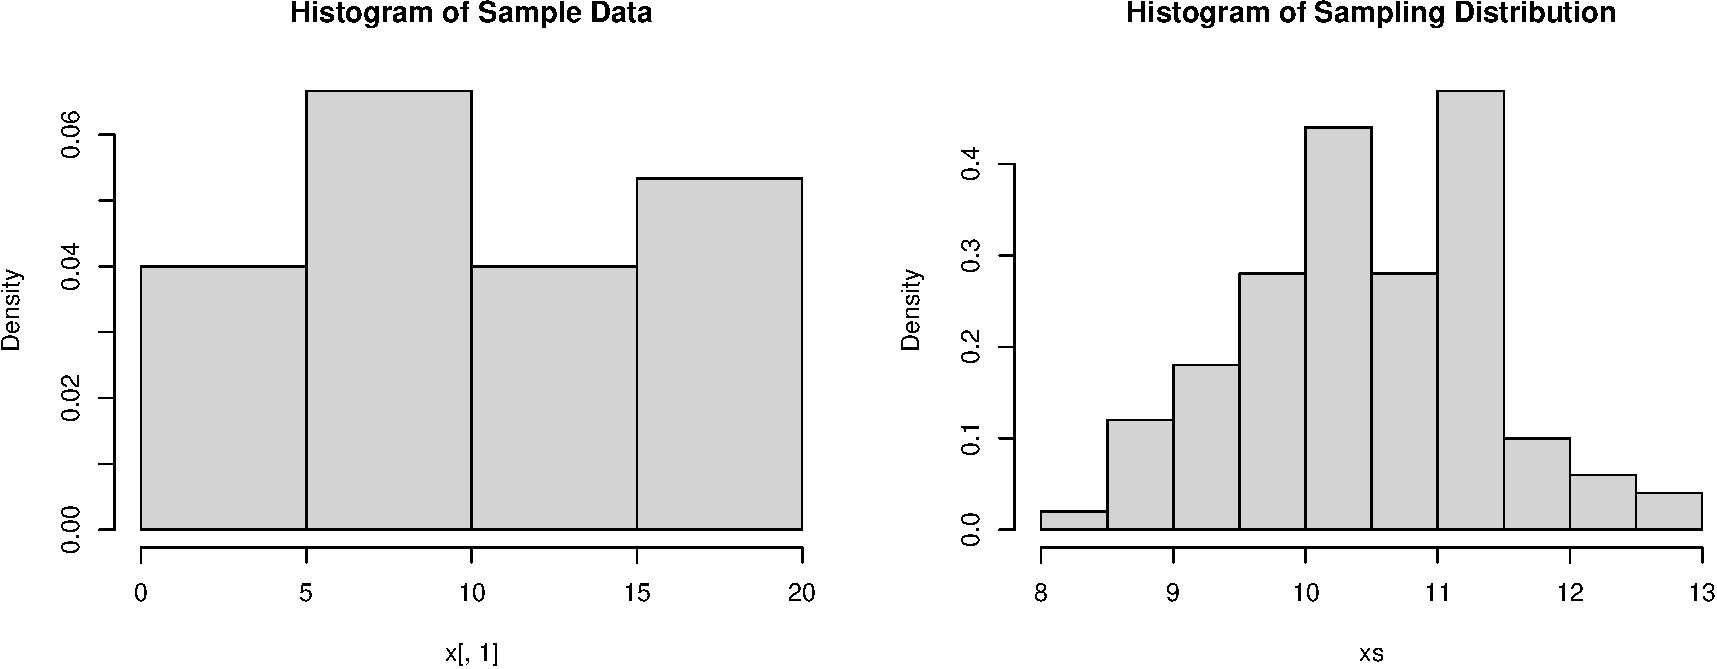
\includegraphics[keepaspectratio]{Lecture-12-Central-Limit-Theorem_files/figure-pdf/unnamed-chunk-8-1.pdf}}

When looking at the results above, it is still difficult to figure out
what distribution the sample data comes from. Even though we know that
it follows a uniform distribution, most of the time we are just given
the data with no knowledge of what distribution it came from. It is
obvious to us though that the sampling distribution is starting to take
shape since we now have 100 values in it. We might be able to see a
normal distribution starting to form. We can also notice that the mean
is roughly the same as the mean of our sample that we found at the very
beginning (10.2), but the standard deviation is much smaller than the
standard deviation of the sample (6.5).

We can repeat this process, but instead of having a sample size of 30 we
can see what happens when we increase the sample size to 100:

\begin{Shaded}
\begin{Highlighting}[]
\NormalTok{x }\OtherTok{\textless{}{-}} \FunctionTok{sample}\NormalTok{(}\DecValTok{1}\SpecialCharTok{:}\DecValTok{20}\NormalTok{, }\DecValTok{100}\NormalTok{, }\AttributeTok{replace=}\ConstantTok{TRUE}\NormalTok{)}
\FunctionTok{mean}\NormalTok{(x)}
\end{Highlighting}
\end{Shaded}

\begin{verbatim}
[1] 10.17
\end{verbatim}

\begin{Shaded}
\begin{Highlighting}[]
\FunctionTok{sd}\NormalTok{(x)}
\end{Highlighting}
\end{Shaded}

\begin{verbatim}
[1] 6.025292
\end{verbatim}

The sample data should look much more like a uniform distribution
(thanks to the Law of Large Numbers). We can see the sampling
distribution again when we take 30 samples with a sample size of 100 and
100 samples with a sample size of 100. When you look at the following
simulations, pay attention to how the standard deviation changes as well
as how the range changes for the sampling distribution.

\begin{Shaded}
\begin{Highlighting}[]
\NormalTok{x }\OtherTok{\textless{}{-}} \FunctionTok{matrix}\NormalTok{(}\FunctionTok{sample}\NormalTok{(}\DecValTok{1}\SpecialCharTok{:}\DecValTok{20}\NormalTok{, }\DecValTok{3000}\NormalTok{, }\AttributeTok{replace=}\ConstantTok{TRUE}\NormalTok{), }\AttributeTok{nrow =} \DecValTok{100}\NormalTok{)}
\NormalTok{xs }\OtherTok{\textless{}{-}} \FunctionTok{apply}\NormalTok{(x, }\DecValTok{2}\NormalTok{, mean)}
\FunctionTok{mean}\NormalTok{(xs)}
\end{Highlighting}
\end{Shaded}

\begin{verbatim}
[1] 10.70167
\end{verbatim}

\begin{Shaded}
\begin{Highlighting}[]
\FunctionTok{sd}\NormalTok{(xs)}
\end{Highlighting}
\end{Shaded}

\begin{verbatim}
[1] 0.4910375
\end{verbatim}

\begin{Shaded}
\begin{Highlighting}[]
\FunctionTok{hist}\NormalTok{(x[,}\DecValTok{1}\NormalTok{], }\AttributeTok{main=}\StringTok{"Histogram of Sample Data"}\NormalTok{, }\AttributeTok{freq=}\ConstantTok{FALSE}\NormalTok{)}
\FunctionTok{hist}\NormalTok{(xs, }\AttributeTok{main=}\StringTok{"Histogram of Sampling Distribution"}\NormalTok{, }\AttributeTok{freq=}\ConstantTok{FALSE}\NormalTok{)}
\end{Highlighting}
\end{Shaded}

\pandocbounded{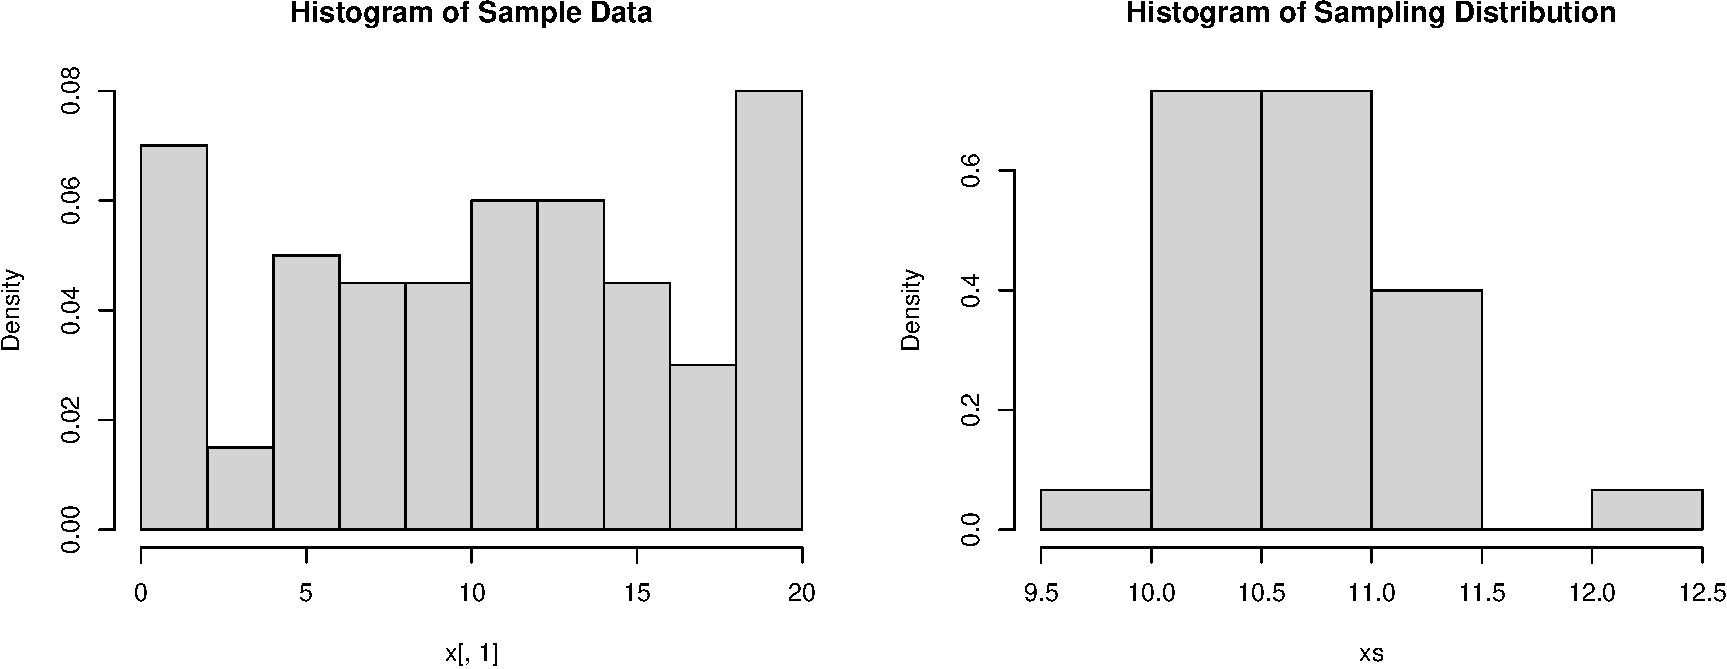
\includegraphics[keepaspectratio]{Lecture-12-Central-Limit-Theorem_files/figure-pdf/unnamed-chunk-12-1.pdf}}

\begin{Shaded}
\begin{Highlighting}[]
\NormalTok{x }\OtherTok{\textless{}{-}} \FunctionTok{matrix}\NormalTok{(}\FunctionTok{sample}\NormalTok{(}\DecValTok{1}\SpecialCharTok{:}\DecValTok{20}\NormalTok{, }\DecValTok{10000}\NormalTok{, }\AttributeTok{replace=}\ConstantTok{TRUE}\NormalTok{), }\AttributeTok{nrow =} \DecValTok{100}\NormalTok{)}
\NormalTok{xs }\OtherTok{\textless{}{-}} \FunctionTok{apply}\NormalTok{(x, }\DecValTok{2}\NormalTok{, mean)}
\FunctionTok{mean}\NormalTok{(xs)}
\end{Highlighting}
\end{Shaded}

\begin{verbatim}
[1] 10.4644
\end{verbatim}

\begin{Shaded}
\begin{Highlighting}[]
\FunctionTok{sd}\NormalTok{(xs)}
\end{Highlighting}
\end{Shaded}

\begin{verbatim}
[1] 0.5447329
\end{verbatim}

\begin{Shaded}
\begin{Highlighting}[]
\FunctionTok{hist}\NormalTok{(x[,}\DecValTok{1}\NormalTok{], }\AttributeTok{main=}\StringTok{"Histogram of Sample Data"}\NormalTok{, }\AttributeTok{freq=}\ConstantTok{FALSE}\NormalTok{)}
\FunctionTok{hist}\NormalTok{(xs, }\AttributeTok{main=}\StringTok{"Histogram of Sampling Distribution"}\NormalTok{, }\AttributeTok{freq=}\ConstantTok{FALSE}\NormalTok{)}
\end{Highlighting}
\end{Shaded}

\pandocbounded{\includegraphics[keepaspectratio]{Lecture-12-Central-Limit-Theorem_files/figure-pdf/unnamed-chunk-15-1.pdf}}

We can notice that the standard deviation is that the only statistic
that really changes each time is the standard deviation. It appears that
the mean of the sample and the mean of the sampling distribution remain
the same but the standard deviation decreases as the sample size gets
larger. We can see the same thing below as we increase the sample size
to 500.

\begin{Shaded}
\begin{Highlighting}[]
\NormalTok{x }\OtherTok{\textless{}{-}} \FunctionTok{sample}\NormalTok{(}\DecValTok{1}\SpecialCharTok{:}\DecValTok{20}\NormalTok{, }\DecValTok{500}\NormalTok{, }\AttributeTok{replace=}\ConstantTok{TRUE}\NormalTok{)}
\FunctionTok{mean}\NormalTok{(x)}
\end{Highlighting}
\end{Shaded}

\begin{verbatim}
[1] 10.514
\end{verbatim}

\begin{Shaded}
\begin{Highlighting}[]
\FunctionTok{sd}\NormalTok{(x)}
\end{Highlighting}
\end{Shaded}

\begin{verbatim}
[1] 5.858878
\end{verbatim}

\begin{Shaded}
\begin{Highlighting}[]
\NormalTok{x }\OtherTok{\textless{}{-}} \FunctionTok{matrix}\NormalTok{(}\FunctionTok{sample}\NormalTok{(}\DecValTok{1}\SpecialCharTok{:}\DecValTok{20}\NormalTok{, }\DecValTok{500}\SpecialCharTok{*}\DecValTok{10}\NormalTok{, }\AttributeTok{replace=}\ConstantTok{TRUE}\NormalTok{), }\AttributeTok{nrow =} \DecValTok{500}\NormalTok{)}
\NormalTok{xs }\OtherTok{\textless{}{-}} \FunctionTok{apply}\NormalTok{(x, }\DecValTok{2}\NormalTok{, mean)}
\FunctionTok{mean}\NormalTok{(xs)}
\end{Highlighting}
\end{Shaded}

\begin{verbatim}
[1] 10.3958
\end{verbatim}

\begin{Shaded}
\begin{Highlighting}[]
\FunctionTok{sd}\NormalTok{(xs)}
\end{Highlighting}
\end{Shaded}

\begin{verbatim}
[1] 0.2366215
\end{verbatim}

\begin{Shaded}
\begin{Highlighting}[]
\FunctionTok{hist}\NormalTok{(x[,}\DecValTok{1}\NormalTok{], }\AttributeTok{main=}\StringTok{"Histogram of Sample Data"}\NormalTok{, }\AttributeTok{freq=}\ConstantTok{FALSE}\NormalTok{)}
\FunctionTok{hist}\NormalTok{(xs, }\AttributeTok{main=}\StringTok{"Histogram of Sampling Distribution"}\NormalTok{, }\AttributeTok{freq=}\ConstantTok{FALSE}\NormalTok{)}
\end{Highlighting}
\end{Shaded}

\pandocbounded{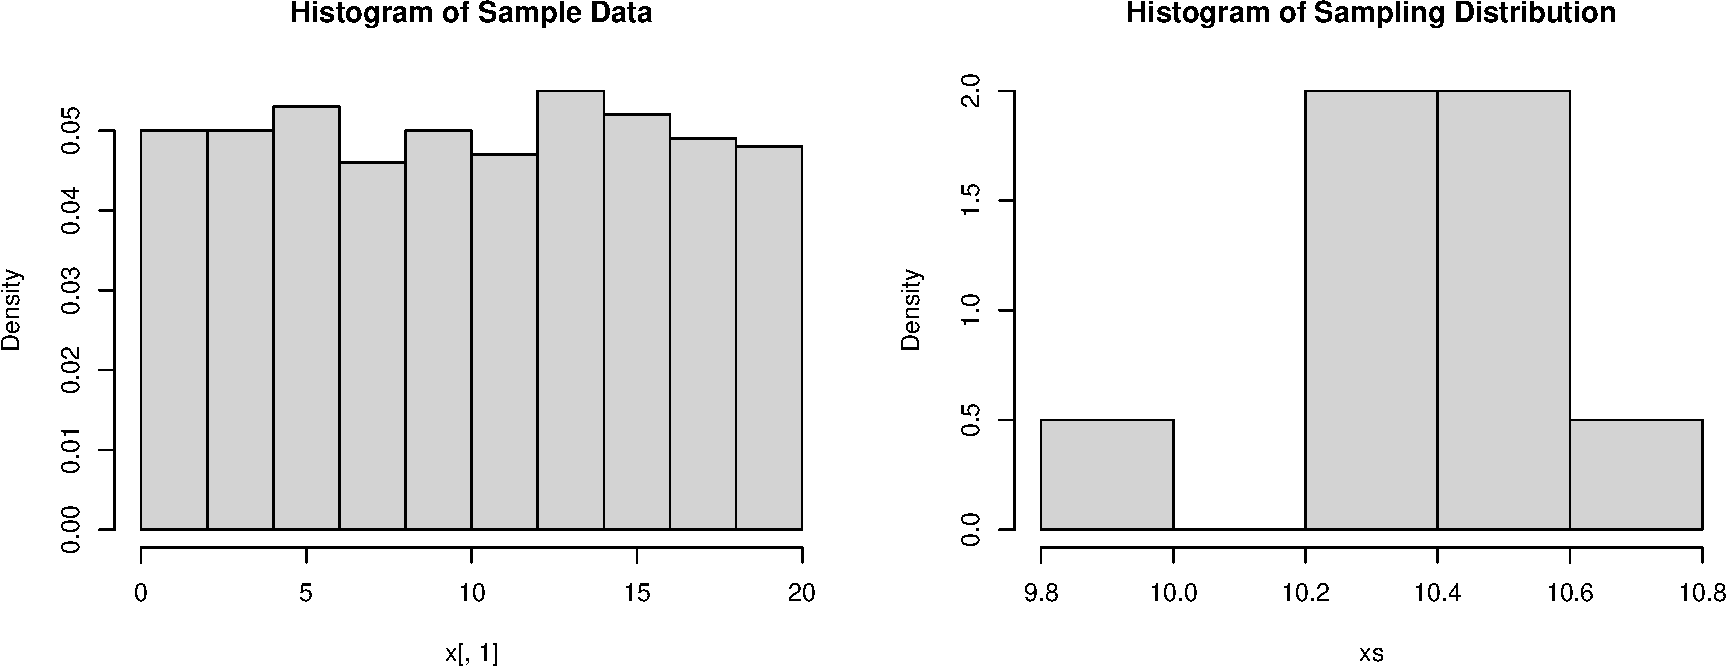
\includegraphics[keepaspectratio]{Lecture-12-Central-Limit-Theorem_files/figure-pdf/unnamed-chunk-19-1.pdf}}

\begin{Shaded}
\begin{Highlighting}[]
\NormalTok{x }\OtherTok{\textless{}{-}} \FunctionTok{matrix}\NormalTok{(}\FunctionTok{sample}\NormalTok{(}\DecValTok{1}\SpecialCharTok{:}\DecValTok{20}\NormalTok{, }\DecValTok{500}\SpecialCharTok{*}\DecValTok{100}\NormalTok{, }\AttributeTok{replace=}\ConstantTok{TRUE}\NormalTok{), }\AttributeTok{nrow =} \DecValTok{500}\NormalTok{)}
\NormalTok{xs }\OtherTok{\textless{}{-}} \FunctionTok{apply}\NormalTok{(x, }\DecValTok{2}\NormalTok{, mean)}
\FunctionTok{mean}\NormalTok{(xs)}
\end{Highlighting}
\end{Shaded}

\begin{verbatim}
[1] 10.43638
\end{verbatim}

\begin{Shaded}
\begin{Highlighting}[]
\FunctionTok{sd}\NormalTok{(xs)}
\end{Highlighting}
\end{Shaded}

\begin{verbatim}
[1] 0.2540353
\end{verbatim}

\begin{Shaded}
\begin{Highlighting}[]
\FunctionTok{hist}\NormalTok{(x[,}\DecValTok{1}\NormalTok{], }\AttributeTok{main=}\StringTok{"Histogram of Sample Data"}\NormalTok{, }\AttributeTok{freq=}\ConstantTok{FALSE}\NormalTok{)}
\FunctionTok{hist}\NormalTok{(xs, }\AttributeTok{main=}\StringTok{"Histogram of Sampling Distribution"}\NormalTok{, }\AttributeTok{freq=}\ConstantTok{FALSE}\NormalTok{)}
\end{Highlighting}
\end{Shaded}

\pandocbounded{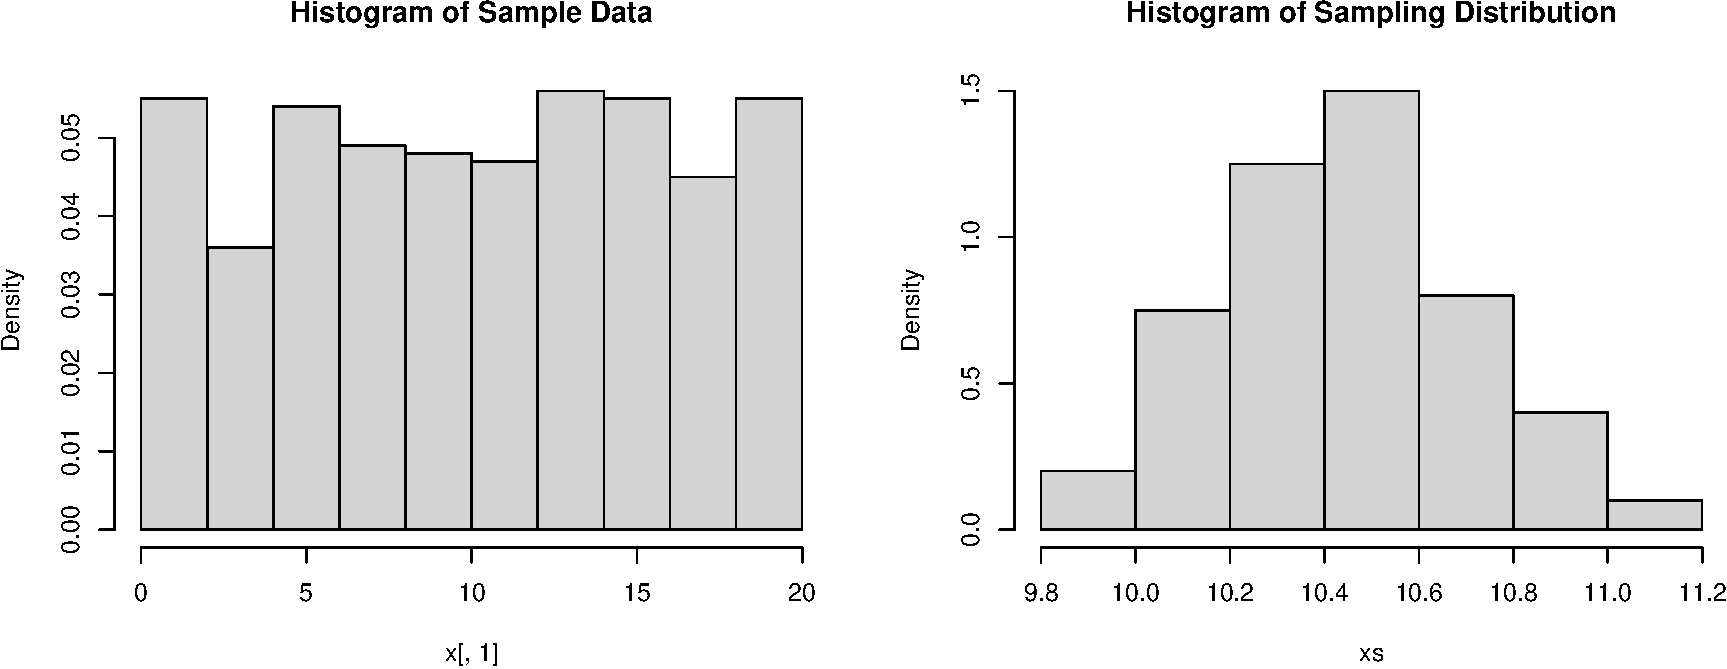
\includegraphics[keepaspectratio]{Lecture-12-Central-Limit-Theorem_files/figure-pdf/unnamed-chunk-22-1.pdf}}

After seeing all of the simulations, we are ready to discuss the
results. We know since we are dealing with a uniform distribution that
the population mean is \(\displaystyle \mu=\frac{1+20}{2}=10.5\) and the
population standard deviation is
\(\displaystyle \sigma = \frac{20-1}{\sqrt{12}}= 5.48\). We can see that
our samples tend to have these results, as the simulation with a sample
size of 500 shows a mean of 10.41 and a standard deviation of 5.78. But,
if you run it again you might get slightly different results.

Through all of the simulations, we can see that the mean of the sampling
distribution is the same as the mean of the population distribution.
With this, we could say that \(E(\bar{X})=\mu_X\). We can also see that
the standard deviation changes as the sample size gets larger. In fact,
we can say that \(\displaystyle SD(\bar{X})=\frac{\sigma}{\sqrt{n}}\).
We can also see that as the sample size increases, the values cluster
more around the mean and we have less variability.

\section{Central Limit Theorem}\label{central-limit-theorem-1}

In fact, this is what the \textbf{Central Limit Theorem} tells us the
distribution of sampling means approximates a normal distribution as the
sample size becomes larger, regardless of the shape of the population
distribution. It also tells us the mean stays the same while the
standard deviation changes based on the size of the sample. This is an
important idea as it shows us that if we have a sample of at least 30,
then no matter what distribution it comes from, the mean of the sample
will follow a normal distribution. This is important in statistics and
data science as the normal distribution is the gold standard which has
very nice properties and is easy to do analysis with.

The Central Limit Theorem even works with highly skewed data. Below is
an example of the gamma distribution. The sample data will be extremely
skewed right, but the sampling distribution of means will exhibit a
normal distribution.

\begin{Shaded}
\begin{Highlighting}[]
\NormalTok{x }\OtherTok{\textless{}{-}} \FunctionTok{matrix}\NormalTok{(}\FunctionTok{rgamma}\NormalTok{(}\DecValTok{500}\SpecialCharTok{*}\DecValTok{1000}\NormalTok{, }\DecValTok{1}\NormalTok{, }\DecValTok{1}\NormalTok{), }\AttributeTok{nrow =} \DecValTok{500}\NormalTok{)}
\NormalTok{xs }\OtherTok{\textless{}{-}} \FunctionTok{apply}\NormalTok{(x, }\DecValTok{2}\NormalTok{, mean)}
\FunctionTok{mean}\NormalTok{(xs)}
\end{Highlighting}
\end{Shaded}

\begin{verbatim}
[1] 1.001284
\end{verbatim}

\begin{Shaded}
\begin{Highlighting}[]
\FunctionTok{sd}\NormalTok{(xs)}
\end{Highlighting}
\end{Shaded}

\begin{verbatim}
[1] 0.04373685
\end{verbatim}

\begin{Shaded}
\begin{Highlighting}[]
\FunctionTok{hist}\NormalTok{(x[,}\DecValTok{1}\NormalTok{], }\AttributeTok{main=}\StringTok{"Histogram of Sample Data"}\NormalTok{, }\AttributeTok{freq=}\ConstantTok{FALSE}\NormalTok{)}
\FunctionTok{hist}\NormalTok{(xs, }\AttributeTok{main=}\StringTok{"Histogram of Sampling Distribution"}\NormalTok{, }\AttributeTok{freq=}\ConstantTok{FALSE}\NormalTok{)}
\end{Highlighting}
\end{Shaded}

\pandocbounded{\includegraphics[keepaspectratio]{Lecture-12-Central-Limit-Theorem_files/figure-pdf/unnamed-chunk-25-1.pdf}}

You might be wondering why it matters still. Well, the Central Limit
Theorem essentially tells us that with a large \(n\), the sampling
distribution of \(\bar{X}\) is normally distributed as
\(\displaystyle N(\mu, \frac{\sigma}{\sqrt{n}})\). This will allow us to
find probabilities easier since
\(\displaystyle P\left( \frac{\bar{X}-\mu}{\sigma/\sqrt{n}}\right) \leq b\)
is \(\displaystyle P(z\leq b)\). We will also see in future lessons that
this makes finding confidence intervals easier as well, whether the
population standard deviations are known or unknown.

\bookmarksetup{startatroot}

\chapter{Confidence Intervals}\label{confidence-intervals}

When we were showing the Central Limit Theorem through simulations, we
were able to generate random samples over and over again to see that the
sampling distribution did follow a normal distribution when the sample
size was sufficiently large. But, in the ``real world'' we are not able
to generate an infinite number of samples, rather we are given a single
sample and told to analyze it and try to figure out what the population
mean is. We will want to come up with a way to state how confident we
are about our estimation of the population mean.

\section{Estimating Parameters}\label{estimating-parameters}

Often we are interested in determining the population mean, and to do
this we have to estimate the population mean (\(\mu\)) with the sample
mean (\(\overline{x}\)). We can see an example of this by generating 10
values from a normal distribution with a mean of 50 and a standard
deviation of 4 and noticing that the sample mean is never exactly the
population mean (50).

\begin{Shaded}
\begin{Highlighting}[]
\FunctionTok{mean}\NormalTok{(}\FunctionTok{rnorm}\NormalTok{(}\DecValTok{10}\NormalTok{,}\DecValTok{50}\NormalTok{,}\DecValTok{4}\NormalTok{))}
\end{Highlighting}
\end{Shaded}

\begin{verbatim}
[1] 48.52402
\end{verbatim}

\begin{Shaded}
\begin{Highlighting}[]
\FunctionTok{mean}\NormalTok{(}\FunctionTok{rnorm}\NormalTok{(}\DecValTok{10}\NormalTok{,}\DecValTok{50}\NormalTok{,}\DecValTok{4}\NormalTok{))}
\end{Highlighting}
\end{Shaded}

\begin{verbatim}
[1] 50.72837
\end{verbatim}

We have seen though that our sample mean will not be the same as our
population mean, so we might want to ask ourselves how confident we are
that the sample mean is the same or close to the population mean. This
is the idea of the confidence interval, as it will allow us to account
for variability and say something like: ``We don't know what the actual
population mean is, but we are pretty sure it is somewhere in between
these two values''.

\section{Central Limit Theorem}\label{central-limit-theorem-2}

In a previous section we saw that the Central Limit Theorem (CLT) says
that as the sample size gets sufficiently large, the sampling
distribution will begin to follow a normal distribution with the
parameters \(N(\mu, \frac{\sigma}{\sqrt{n}})\). The issue is when we are
given a sample is that we don't know what \(\mu\) is, so we have to
estimate it using the sample mean. We will also need to account for the
variability of our estimate, which can be done using the standard error.

To estimate it and give ourselves a little ``buffer room'', we will need
to create an interval that allows for some variability with our sample.
Since the sampling distribution will follow a normal distribution, we
can use the \(68-95-99,7\) rule to assist us. If we remember correctly,
\(68\%\) of the data will be within 1 standard deviation, \(95\%\) of
the data will be within 2 standard deviations, and \(99.7\%\) of the
data will be within 3 standard deviations. Since we know that \(68\%\)
of the data is within one standard deviation of the mean, we can
essentially infer that the population mean lies within 1 standard
deviation of the sample \(68\%\) of the time. And since we are
discussing the sampling distribution, we know the standard deviation is
scaled to \(\frac{\sigma}{\sqrt{n}}\), which we will call the standard
error (SE).

\section{\texorpdfstring{Creating Confidence Intervals when \(\sigma\)
is
known}{Creating Confidence Intervals when \textbackslash sigma is known}}\label{creating-confidence-intervals-when-sigma-is-known}

We can create a confidence interval using this idea. For instance, if we
wanted to create a 68\% Confidence Interval then since we know 68\% of
the data will lie within 1 standard error we could write it as:

\[ \overline{x} \pm \text{SE} = (\overline{x} - \text{SE}, \overline{x} + \text{SE}) \]

For instance, if we had a sample mean of 50 and a standard error of 5,
then the 68\% Confidence Interval would be \((45,55)\). If we wanted a
95\% Confidence Interval then we would need to multiply the standard
error by 2, giving us \((40,60)\). It should be mentioned that the
standard error relies on both the population standard deviation
(\(\sigma\)) and the sample size (\(n\)). If one is altered then the
standard error will change and will either ``widen'' the confidence
interval or cause it to become more ``narrow''.

Now we can easily create \(68\%\), \(95\%\), and \(99,7\%\) Confidence
Intervals by multiplying the standard error by 1, 2, and 3 respectively.
But, what if we want some other level of confidence instead? Well, we
could find the \(z-\)score associated with the particular level of
confidence by drawing ourselves a picture. This will allow us to scale
the standard error by the correct value. If we wanted to create a
\(90\%\) Confidence Interval then we need to find the \(z-\)score where
\(90\%\) of the data is between it.

\begin{center}
\pandocbounded{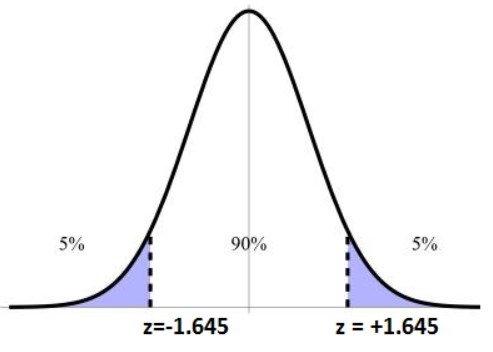
\includegraphics[keepaspectratio]{images/L13-z-score.png}}
\end{center}

To find these values, we can use the \(qnorm()\) function which will
find the \(z-\)score which has the inputted value of data to the left of
the point. So, if we wanted to find the \(z-\)score for the \(90\%\)
confidence interval then we would want to find the value where \(95\%\)
of the data is to the left of it:

\begin{Shaded}
\begin{Highlighting}[]
\FunctionTok{qnorm}\NormalTok{(.}\DecValTok{95}\NormalTok{)}
\end{Highlighting}
\end{Shaded}

\begin{verbatim}
[1] 1.644854
\end{verbatim}

With this, we can officially define the confidence interval as:

\[ \overline{x} \pm z_{*} \frac{\sigma}{\sqrt{n}} = \left(\overline{x} -  z_{*} \frac{\sigma}{\sqrt{n}} ,\overline{x} +  z_{*} \frac{\sigma}{\sqrt{n}} \right) \]

where \(z_*\) changes based on the level of confidence one wants.

\subsection{An Example of Confidence
Intervals}\label{an-example-of-confidence-intervals}

Let's create a single sample coming from a normal distribution with the
sample size being 30, a mean of 10, and a standard deviation of 5. We
can create a \(95\%\) confidence interval as follows:

\begin{Shaded}
\begin{Highlighting}[]
\NormalTok{x }\OtherTok{\textless{}{-}} \FunctionTok{rnorm}\NormalTok{(}\DecValTok{30}\NormalTok{, }\DecValTok{10}\NormalTok{, }\DecValTok{5}\NormalTok{)}
\NormalTok{se }\OtherTok{\textless{}{-}} \DecValTok{5}\SpecialCharTok{/}\FunctionTok{sqrt}\NormalTok{(}\DecValTok{30}\NormalTok{)}
\NormalTok{z }\OtherTok{\textless{}{-}} \FunctionTok{qnorm}\NormalTok{(.}\DecValTok{975}\NormalTok{)}
\FunctionTok{mean}\NormalTok{(x) }\SpecialCharTok{+} \FunctionTok{c}\NormalTok{(}\SpecialCharTok{{-}}\DecValTok{1}\NormalTok{,}\DecValTok{1}\NormalTok{)}\SpecialCharTok{*}\NormalTok{z}\SpecialCharTok{*}\NormalTok{se}
\end{Highlighting}
\end{Shaded}

\begin{verbatim}
[1]  7.975287 11.553675
\end{verbatim}

In the code above we got a 95\% confidence interval of (7.975, 11.554).
If we were to repeat the process, we might get something that looks
completely different:

\begin{Shaded}
\begin{Highlighting}[]
\NormalTok{x }\OtherTok{\textless{}{-}} \FunctionTok{rnorm}\NormalTok{(}\DecValTok{30}\NormalTok{, }\DecValTok{10}\NormalTok{, }\DecValTok{5}\NormalTok{)}
\NormalTok{se }\OtherTok{\textless{}{-}} \DecValTok{5}\SpecialCharTok{/}\FunctionTok{sqrt}\NormalTok{(}\DecValTok{30}\NormalTok{)}
\NormalTok{z }\OtherTok{\textless{}{-}} \FunctionTok{qnorm}\NormalTok{(.}\DecValTok{975}\NormalTok{)}
\FunctionTok{mean}\NormalTok{(x) }\SpecialCharTok{+} \FunctionTok{c}\NormalTok{(}\SpecialCharTok{{-}}\DecValTok{1}\NormalTok{,}\DecValTok{1}\NormalTok{)}\SpecialCharTok{*}\NormalTok{z}\SpecialCharTok{*}\NormalTok{se}
\end{Highlighting}
\end{Shaded}

\begin{verbatim}
[1]  9.102498 12.680886
\end{verbatim}

If you repeat this process 100 times in total, then 95\% of your
confidence intervals will contain the true population mean (of 10).
Normally though, we don't know the true population mean. Below is
another example which we might encounter:

Suppose you are interested in determining the weekly average price of
groceries for a family of 4. You collect a sample of 40 families and
determine the average price is \$125 and you know from an earlier study
that the population standard deviation is \$55. Construct a 90\% CI and
a 95\% CI.

\begin{Shaded}
\begin{Highlighting}[]
\NormalTok{xbar }\OtherTok{\textless{}{-}} \DecValTok{125}
\NormalTok{se }\OtherTok{\textless{}{-}} \DecValTok{55}\SpecialCharTok{/}\FunctionTok{sqrt}\NormalTok{(}\DecValTok{40}\NormalTok{)}
\NormalTok{z }\OtherTok{\textless{}{-}} \FunctionTok{qnorm}\NormalTok{(.}\DecValTok{95}\NormalTok{) }\CommentTok{\# z{-}score for 90\% CI}
\NormalTok{xbar }\SpecialCharTok{+} \FunctionTok{c}\NormalTok{(}\SpecialCharTok{{-}}\DecValTok{1}\NormalTok{,}\DecValTok{1}\NormalTok{)}\SpecialCharTok{*}\NormalTok{z}\SpecialCharTok{*}\NormalTok{se}
\end{Highlighting}
\end{Shaded}

\begin{verbatim}
[1] 110.6959 139.3041
\end{verbatim}

\begin{Shaded}
\begin{Highlighting}[]
\NormalTok{z }\OtherTok{\textless{}{-}} \FunctionTok{qnorm}\NormalTok{(.}\DecValTok{975}\NormalTok{) }\CommentTok{\# z{-}score for 95\% CI}
\NormalTok{xbar }\SpecialCharTok{+} \FunctionTok{c}\NormalTok{(}\SpecialCharTok{{-}}\DecValTok{1}\NormalTok{,}\DecValTok{1}\NormalTok{)}\SpecialCharTok{*}\NormalTok{z}\SpecialCharTok{*}\NormalTok{se}
\end{Highlighting}
\end{Shaded}

\begin{verbatim}
[1] 107.9556 142.0444
\end{verbatim}

This shows us that, while we don't know what the true population mean
is, we can be 90\% confident that the population mean is somewhere
between (\$110.70, \$139.30) and 95\% confident it is between (\$107.96,
\$142.04). We should note that we do not want to say that the
probability is 90\% or 95\%, but rather if we were to repeat the sample
100 times, then 90\% and 95\% of the confidence intervals should contain
the population mean.

\section{\texorpdfstring{Creating Confidence Intervals when \(\sigma\)
is
unknown}{Creating Confidence Intervals when \textbackslash sigma is unknown}}\label{creating-confidence-intervals-when-sigma-is-unknown}

In the examples above, we were able to assume that we knew the
population standard deviation, but often we don't know that. We are
usually just given the sample without knowing anything about the
population mean or standard deviation, so we have to estimate both of
those to infer things about the sample. But, estimating both of these
parameters gives us more chances to be wrong. Therefore, we want to give
ourselves a little wider confidence interval in order to account for
this. Since we have more chances of being wrong, we will want to pull
the \(z-\)score from something that stretches out a little further than
a normal distribution. This will allow us to scale the standard error by
a slightly larger number to account for the chances of being wrong. To
do this, we will use what is called a Student's t-distribution. This
looks very much like a normal distribution but has thicker tails. As the
sample size increases the distribution becomes more and more like a
normal distribution.

\begin{center}
\pandocbounded{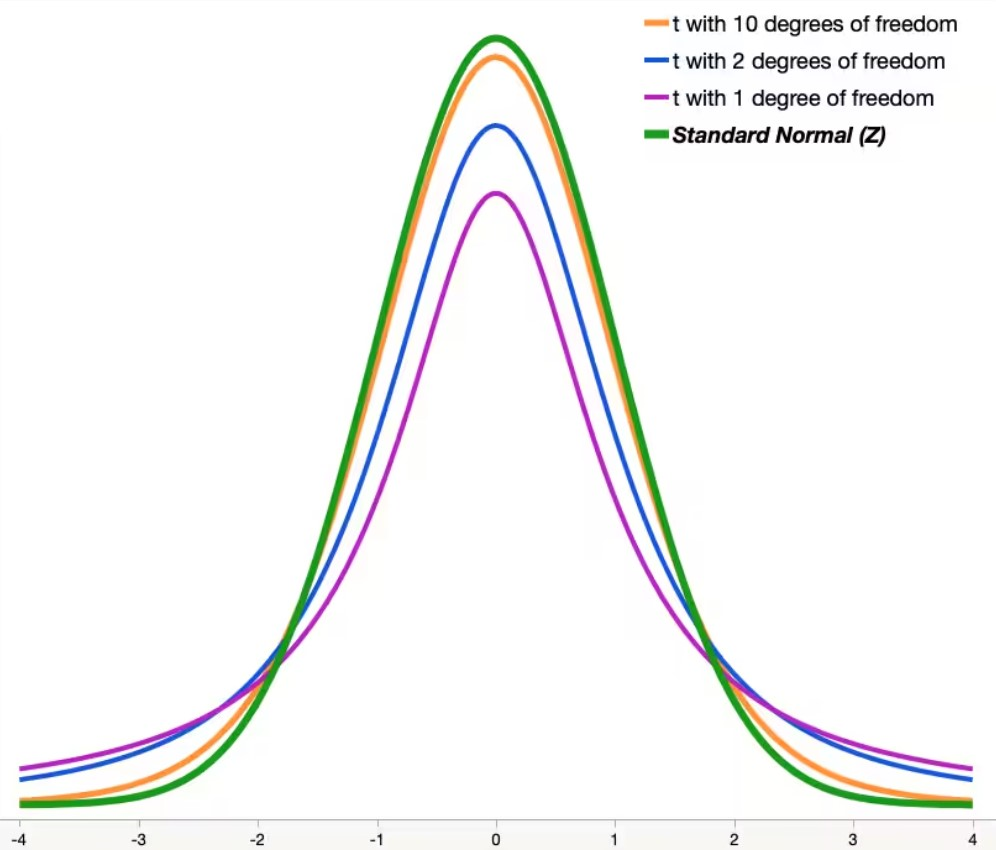
\includegraphics[keepaspectratio]{images/L13-t-distribution.png}}
\end{center}

The degree of freedom is the sample size minus 1 (\(df=n-1\)). In the
picture above we can see that when the degrees of freedom are small then
we have thicker tails than a normal distribution, this will cause the
quantiles for a confidence interval to be larger than a normal
distribution. We can see this in action if we use the \(qt()\) function
instead of the \(qnorm()\) function. Notice how the amount we will scale
the standard error by gets closer to the normal distribution as the
sample size (and degrees of freedom) gets large.

\begin{Shaded}
\begin{Highlighting}[]
\FunctionTok{qt}\NormalTok{(.}\DecValTok{95}\NormalTok{, }\AttributeTok{df=}\DecValTok{2}\NormalTok{)}
\end{Highlighting}
\end{Shaded}

\begin{verbatim}
[1] 2.919986
\end{verbatim}

\begin{Shaded}
\begin{Highlighting}[]
\FunctionTok{qt}\NormalTok{(.}\DecValTok{95}\NormalTok{, }\AttributeTok{df=}\DecValTok{10}\NormalTok{)}
\end{Highlighting}
\end{Shaded}

\begin{verbatim}
[1] 1.812461
\end{verbatim}

\begin{Shaded}
\begin{Highlighting}[]
\FunctionTok{qt}\NormalTok{(.}\DecValTok{95}\NormalTok{, }\AttributeTok{df=}\DecValTok{1000}\NormalTok{)}
\end{Highlighting}
\end{Shaded}

\begin{verbatim}
[1] 1.646379
\end{verbatim}

\begin{Shaded}
\begin{Highlighting}[]
\FunctionTok{qnorm}\NormalTok{(.}\DecValTok{95}\NormalTok{)}
\end{Highlighting}
\end{Shaded}

\begin{verbatim}
[1] 1.644854
\end{verbatim}

When creating the confidence interval, everything is the same as before
except now we will use the sample standard deviation (\(s\)) to estimate
the population standard deviation (\(\sigma\)) and we will use the
\(t-\)score instead of the \(z-\)score. Below is the general form:

\[ \overline{x} \pm t_*\frac{s}{\sqrt{n}} = \left(\overline{x} - t_*\frac{s}{\sqrt{n}},\overline{x} + t_*\frac{s}{\sqrt{n}}\right) \]

Let's look at an example of when we take a sample of size 10 from a
normal distribution with a mean of 10 and a standard deviation of 5. If
we know the population standard deviation then we can do the confidence
interval like we have before, but if we do not know the population
standard deviation then we need to use the methods just discussed

\begin{Shaded}
\begin{Highlighting}[]
\NormalTok{x }\OtherTok{\textless{}{-}} \FunctionTok{rnorm}\NormalTok{(}\DecValTok{10}\NormalTok{,}\DecValTok{10}\NormalTok{,}\DecValTok{5}\NormalTok{)}

\CommentTok{\# Assuming we know the population standard deviation}
\NormalTok{se }\OtherTok{\textless{}{-}} \DecValTok{5}\SpecialCharTok{/}\FunctionTok{sqrt}\NormalTok{(}\DecValTok{10}\NormalTok{)}
\NormalTok{z }\OtherTok{\textless{}{-}} \FunctionTok{qnorm}\NormalTok{(.}\DecValTok{975}\NormalTok{)}
\FunctionTok{mean}\NormalTok{(x) }\SpecialCharTok{+} \FunctionTok{c}\NormalTok{(}\SpecialCharTok{{-}}\DecValTok{1}\NormalTok{,}\DecValTok{1}\NormalTok{)}\SpecialCharTok{*}\NormalTok{z}\SpecialCharTok{*}\NormalTok{se}
\end{Highlighting}
\end{Shaded}

\begin{verbatim}
[1]  7.516443 13.714394
\end{verbatim}

\begin{Shaded}
\begin{Highlighting}[]
\CommentTok{\# Assuming we do not know the population standard deviation}
\NormalTok{se }\OtherTok{\textless{}{-}} \FunctionTok{sd}\NormalTok{(x)}\SpecialCharTok{/}\FunctionTok{sqrt}\NormalTok{(}\DecValTok{10}\NormalTok{)}
\NormalTok{t }\OtherTok{\textless{}{-}} \FunctionTok{qt}\NormalTok{(.}\DecValTok{975}\NormalTok{, }\AttributeTok{df=}\DecValTok{10{-}1}\NormalTok{)}
\FunctionTok{mean}\NormalTok{(x) }\SpecialCharTok{+} \FunctionTok{c}\NormalTok{(}\SpecialCharTok{{-}}\DecValTok{1}\NormalTok{,}\DecValTok{1}\NormalTok{)}\SpecialCharTok{*}\NormalTok{t}\SpecialCharTok{*}\NormalTok{se}
\end{Highlighting}
\end{Shaded}

\begin{verbatim}
[1]  7.266145 13.964692
\end{verbatim}

In this case, we can see that the new confidence interval is more narrow
than the first confidence interval. And that is because the standard
deviation fluctuates greatly since we have so few observations. Here we
can see that the standard deviation of the data is roughly half what we
would expect it to be, causing the SE to be smaller and thus a more
narrow confidence interval. But if we do it again then the confidence
interval might be wider.

\begin{Shaded}
\begin{Highlighting}[]
\FunctionTok{sd}\NormalTok{(x)}
\end{Highlighting}
\end{Shaded}

\begin{verbatim}
[1] 4.681961
\end{verbatim}

\begin{Shaded}
\begin{Highlighting}[]
\NormalTok{x }\OtherTok{\textless{}{-}} \FunctionTok{rnorm}\NormalTok{(}\DecValTok{10}\NormalTok{,}\DecValTok{10}\NormalTok{,}\DecValTok{5}\NormalTok{)}
\FunctionTok{sd}\NormalTok{(x)}
\end{Highlighting}
\end{Shaded}

\begin{verbatim}
[1] 4.977537
\end{verbatim}

\begin{Shaded}
\begin{Highlighting}[]
\FunctionTok{mean}\NormalTok{(x) }\SpecialCharTok{+} \FunctionTok{c}\NormalTok{(}\SpecialCharTok{{-}}\DecValTok{1}\NormalTok{,}\DecValTok{1}\NormalTok{)}\SpecialCharTok{*}\NormalTok{t}\SpecialCharTok{*}\FunctionTok{sd}\NormalTok{(x)}\SpecialCharTok{/}\FunctionTok{sqrt}\NormalTok{(}\DecValTok{10}\NormalTok{)}
\end{Highlighting}
\end{Shaded}

\begin{verbatim}
[1]  4.624695 11.746127
\end{verbatim}

Now we know that the sampling distribution will approach a normal
distribution as the sample size gets sufficiently large. This allows us
to use the \(z-\)score to scale the standard error when we know the
population standard deviation. But, since we are using the
\(t-\)distribution then we can't quite use the Central Limit Theorem
exactly. For our purposes, we will say that we can use the
\(t-\)distribution when the absolute value of the skew is as follows:
\textbf{(a)} \(|\text{skew}|< 0.5\) then \(n>15\), \textbf{(b)}
\(|\text{skew}|< 1.0\) then \(n>30\), and \(|\text{skew}|> 1.0\) then
\(n>60\). This is because we know that we require larger sample sizes
for the sampling distribution to look symmetrical when the data is
heavily skewed.

Let's look at an example of something we might encounter while working
on a problem. We will use the `absenteeism' dataset in the `openintro'
library and construct a \(95\%\) confidence interval for the mean number
of days missed. We can also see that a function exists in R that will
virtually calculate it for us, though we want to only use it to verify
our results for now:

\begin{Shaded}
\begin{Highlighting}[]
\FunctionTok{library}\NormalTok{(openintro)}
\end{Highlighting}
\end{Shaded}

\begin{verbatim}
Warning: package 'openintro' was built under R version 4.3.3
\end{verbatim}

\begin{verbatim}
Loading required package: airports
\end{verbatim}

\begin{verbatim}
Loading required package: cherryblossom
\end{verbatim}

\begin{verbatim}
Loading required package: usdata
\end{verbatim}

\begin{verbatim}
Warning: package 'usdata' was built under R version 4.3.3
\end{verbatim}

\begin{Shaded}
\begin{Highlighting}[]
\NormalTok{x }\OtherTok{\textless{}{-}}\NormalTok{ absenteeism}\SpecialCharTok{$}\NormalTok{days }\CommentTok{\# Just so I dont have to keep rewriting it}
\FunctionTok{mean}\NormalTok{(x) }\SpecialCharTok{+} \FunctionTok{c}\NormalTok{(}\SpecialCharTok{{-}}\DecValTok{1}\NormalTok{,}\DecValTok{1}\NormalTok{)}\SpecialCharTok{*}\FunctionTok{qt}\NormalTok{(.}\DecValTok{975}\NormalTok{, }\AttributeTok{df=}\FunctionTok{length}\NormalTok{(x)}\SpecialCharTok{{-}}\DecValTok{1}\NormalTok{)}\SpecialCharTok{*}\FunctionTok{sd}\NormalTok{(x)}\SpecialCharTok{/}\FunctionTok{sqrt}\NormalTok{(}\FunctionTok{length}\NormalTok{(x))}
\end{Highlighting}
\end{Shaded}

\begin{verbatim}
[1] 13.80032 19.11749
\end{verbatim}

\begin{Shaded}
\begin{Highlighting}[]
\FunctionTok{t.test}\NormalTok{(x, }\AttributeTok{conf.level =}\NormalTok{ .}\DecValTok{95}\NormalTok{)}\SpecialCharTok{$}\NormalTok{conf.int}
\end{Highlighting}
\end{Shaded}

\begin{verbatim}
[1] 13.80032 19.11749
attr(,"conf.level")
[1] 0.95
\end{verbatim}

\section{Confidence Intervals for Categorical
Data}\label{confidence-intervals-for-categorical-data}

So far we have seen how we can make confidence intervals for
quantitative data, but what if we have qualitative data instead? Well,
it turns out that the Central Limit Theorem applies to that as well. If
we have categorical data that can be written as Success and Failure then
the proportion of successes will be
\(\hat{p}=\frac{\# \text{ of successes}}{\# \text{ of total values}}\).
The standard error cannot be found by taking the standard deviation,
rather it will be \(\text{SE}=\sqrt{\frac{p(1-p)}{n}}\). This will work
as long as our observations are independent of each other and as long as
\(np\geq 5\) and \(n(1-p)\geq 5\). When the population proportion
(\(p\)) is not known then we will use \(\hat{p}\) to estimate it.

The general form of the confidence interval will use the normal
distribution to scale the standard error and it will be of the following
form:

\[ \hat{p} \pm z_* \sqrt{\frac{\hat{p}(1-\hat{p})}{n}} = \left(\hat{p} - z_* \sqrt{\frac{\hat{p}(1-\hat{p})}{n}}, \hat{p} + z_* \sqrt{\frac{\hat{p}(1-\hat{p})}{n}}\right) \]

To see this in practice we will look at the same `absenteeism' dataset
in the `openintro' library. We will want to create a \(95\%\) confidence
interval for the proportion of males classified as having chronic
absences. There are functions in R that will calculate it for us similar
to the \(t.test()\) but we will just write it out for now.

\begin{Shaded}
\begin{Highlighting}[]
\FunctionTok{table}\NormalTok{(absenteeism}\SpecialCharTok{$}\NormalTok{sex)}
\end{Highlighting}
\end{Shaded}

\begin{verbatim}

 F  M 
80 66 
\end{verbatim}

\begin{Shaded}
\begin{Highlighting}[]
\NormalTok{phat }\OtherTok{\textless{}{-}} \DecValTok{66}\SpecialCharTok{/}\FunctionTok{length}\NormalTok{(absenteeism}\SpecialCharTok{$}\NormalTok{sex)}
\NormalTok{se }\OtherTok{\textless{}{-}} \FunctionTok{sqrt}\NormalTok{(phat}\SpecialCharTok{*}\NormalTok{(}\DecValTok{1}\SpecialCharTok{{-}}\NormalTok{phat)}\SpecialCharTok{/}\FunctionTok{length}\NormalTok{(absenteeism}\SpecialCharTok{$}\NormalTok{sex))}
\NormalTok{phat }\SpecialCharTok{+} \FunctionTok{c}\NormalTok{(}\SpecialCharTok{{-}}\DecValTok{1}\NormalTok{,}\DecValTok{1}\NormalTok{)}\SpecialCharTok{*}\FunctionTok{qnorm}\NormalTok{(.}\DecValTok{975}\NormalTok{)}\SpecialCharTok{*}\NormalTok{se}
\end{Highlighting}
\end{Shaded}

\begin{verbatim}
[1] 0.3713246 0.5327849
\end{verbatim}

\bookmarksetup{startatroot}

\chapter{Hypothesis Testing}\label{hypothesis-testing}

Confidence Intervals and Hypothesis Testing both allow us to make
inferences about a population using just the sample. With this, we can
predict the likelihood of population values and state confidence in our
results. We have seen that the confidence interval lets us say something
along the lines of: ``We are pretty certain the population mean is
within this interval''. Hypothesis testing will allow us to do something
similar, but instead, we will be able to compare our sample value to the
claimed population value.

\section{Hypothesis Testing}\label{hypothesis-testing-1}

To perform a hypothesis test, we first have to make a claim about the
population. This is what we will call the hypothesis. The null
hypothesis (written as \(H_0\)) means there is no difference in the data
while the alternative hypothesis (written as \(H_A\)) indicates there is
a difference in the data. For instance, if we are interested in seeing
if the mean is different than 7 then our starting assumption will be
\(H_0: \mu= 82.3\) while the alternative hypothesis will be
\(H_A: \mu \neq 82.3\). Another example is the judicial system in the
United States. The idea is built on the premise that all suspects are
innocent unless proven guilty. So, the starting assumption is that the
client is innocent and it is the prosecutor's job to convince us
otherwise. Therefore, the null hypothesis will be
\(H_0: \text{Innocent}\) while the alternative hypothesis will be
\(H_A: \text{Guilty}\).

It is vital to realize that there are only 2 conclusions we can make in
hypothesis testing. The first is that we can reject the null hypothesis
in favor of the alternative hypothesis and the second is that we can
fail to reject the null hypothesis. Failing to reject the null
hypothesis means that there is no evidence to suggest the initial claim
is wrong. What we can never do though is to accept the null hypothesis.
Going back to our court example might help us realize this. When the
jury comes back after deliberations they either proclaim the defendant
is guilty (they have rejected the null hypothesis and said that there is
enough evidence to say they are not innocent) or the defendant is not
guilty (they have failed to reject the null hypothesis and said they do
not have enough evidence to say the defendant is guilty). What they do
not do is accept the null hypothesis, that is they do not proclaim the
defendant innocent (as they can never be 100\% sure), all they can do is
say that enough evidence has been produced to show them guilty or enough
evidence has not been produced to show them guilty.

The way we will do hypothesis testing is similar to confidence
intervals, and they are both interconnected. Let's look at a normal
distribution centered around the population mean (which is usually the
null hypothesis). We know from the previous sections that if we take a
bunch of samples from the population, \(95\%\) of the sample means will
fall in the ``white'' region while \(5\%\) of the sample means will fall
in the ``blue'' region. If our sample mean falls in the ``blue'' region
and is far away from the population mean, we will usually pause and
question whether our sample actually came from the same population or
not, as it is unlikely to be far away from \(\mu\). We could just have
an unlucky sample, as it does fall in the blue region \(5\%\) of the
time though.

\begin{center}
\pandocbounded{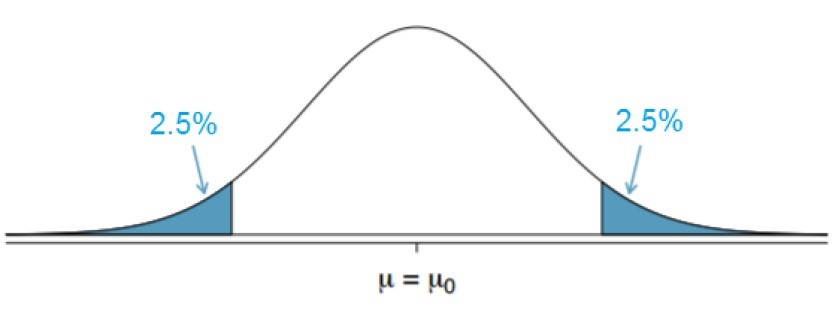
\includegraphics[keepaspectratio]{images/L14-95-conf-int.png}}
\end{center}

There are a few pieces of information that should be addressed before
actually carrying out our hypothesis test. The first is the significance
level (\(\alpha\)), and this will identify the region where the
probability of observing values under the null hypothesis is \(\alpha\).
In this class we will have the significance level be \(5\%\), meaning
\(\alpha/2 = 2.5\%\) is on each side. The ``blue'' sections are the area
beyond the quantile associated with specified significance levels and we
will call this the rejection region. If our value falls in the rejection
region then we will reject the null hypothesis. Since we normally deal
with the standard normal distribution, we will want to normalize our
value, and we will call this our test statistic. The test statistic can
be found in the following way:

\[ \text{test statistic} = \frac{\text{observed - hypothesis}}{\text{standard error}} \]

The last important piece of the puzzle for us is the idea of the
\(p-\)value. This \(p-\)value is the probability of observing a data
value as or more extreme than the test statistic if the null hypothesis
was true at the time. This will help us see if the sample mean occurred
by chance or if it was highly unlikely to occur by chance then we might
say the null hypothesis was not true. Particularly, if the \(p-\)value
\(<\) significance level then we will reject the null hypothesis, and if
the \(p-\)value \(>\) significance level then we will fail to reject the
null hypothesis.

There are different types of hypothesis tests out there. In this class
we will just be looking at the two-sided tests, meaning \(\alpha/2\) is
on each side. This will also result in the null hypothesis always having
equality and the alternative hypothesis being not equal to. You may wish
to do a one-sided test and have the alternative hypothesis be less than
or greater than some value, in which you will have to alter your
rejection region to have \(\alpha\) on one side. But, to find the
\(p-\)value we can use the \(pnorm()\) and the \(pt()\) functions
similar to how we used the \(qnorm()\) and the \(qt()\) in previous
lessons. The general steps for hypothesis testing can be found below,
with it working the same way for means and proportions:

\begin{enumerate}
\def\labelenumi{\arabic{enumi}.}
\tightlist
\item
  Formulate your Hypothesis
\item
  Validate assumptions similar to confidence intervals
\item
  Calculate the Standard Error
\item
  Calculate the Test Statistic
\item
  Calculate the \(p-\)value
\item
  Compare the \(p-\)value to the significance level
\end{enumerate}

Let's look at a few examples and run through the process of hypothesis
testing. The nutrition label on a bag of potato chips says that a
one-ounce (28-grams) serving of potato chips has 130 calories with a
standard deviation of 17. A random sample of 35 bags yielded a sample
mean of 134 calories. Is there evidence that the nutrition label does
not provide an accurate measure of calories in the bags of potato chips?

Our first step is to formulate our hypothesis, and since we want to see
if the calories are correct on the bag then we will want to use that.
The starting assumption is that there are 130 calories in the bag and we
want to test this claim. This gives us the following setup:

\[ H_0: \mu = 130 \\ H_A: \mu \neq 130\]

Now we will want to calculate the standard error. Since we know the
population standard deviation (\(\sigma = 17\)) then we can use
\(\text{SE}=\frac{\sigma}{\sqrt{n}}\), where \(n\) is the sample size.
This gives us: \[ \text{SE} = \frac{17}{\sqrt{35}} \approx 2.874 \]

We can see how many standard errors our observation was off by
calculating the test statistic. We observed the sample mean to be 134,
so we can find the test statistic as:
\[ \text{test statistic} = t = \frac{\text{observed - hypothesis}}{\text{SE}} = \frac{134-130}{2.874} \approx 1.392\]

So, our test statistic is 1.392 standard errors above the mean. If we
were to draw a picture we could visualize the rejection regions to
determine what the outcome of our hypothesis test would be. Since we
have a known population standard deviation then the rejection region
would be less than \(qnorm(.025)=-1.96\) and greater than
\(qnorm(0.975)=1.96\). Since the test statistic does not fall in the
rejection region then we will fail to reject the null hypothesis. But
lets look at the \(p-\)value to confirm this thought process.

To do this, going back to our picture might help. We will want to see
the probability of being more extreme than the test statistic. So, we
will need to see the probability of being greater than 1.392 and less
than -1.392. To do this we will use the \(pnorm()\) function. This will
tell us the probability of being less than a value, so if we want to
find the probability of being greater than the value then we will need
to do \(1 - pnorm()\). We can then double this value since it is
symmetric to get the p-value.

\begin{Shaded}
\begin{Highlighting}[]
\NormalTok{(}\DecValTok{1}\SpecialCharTok{{-}}\FunctionTok{pnorm}\NormalTok{(}\FloatTok{1.392}\NormalTok{))}\SpecialCharTok{*}\DecValTok{2}
\end{Highlighting}
\end{Shaded}

\begin{verbatim}
[1] 0.1639224
\end{verbatim}

Because the \(p-\)value of 0.164 \(> alpha\) (0.05) we will fail to
reject the null hypothesis. That is, we do not have enough evidence to
suggest that the mean number of calories is different than 130. We are
not saying the mean is 130, just that we don't have enough evidence to
suggest it isn't 130.

Let's look at another example. In the 1990s, doctors claimed the mean
birth weight of babies was 7.3 pounds (don't quote me on this as I made
it up). Using the `births' dataset in the `openintro' library run a
hypothesis test to see if the mean weight is different than 7.3 pounds.
So, when we formulate our hypothesis we are told that the mean weight is
7.3 pounds, so this is our starting assumption. This gives us the
following setup:

\[ H_0: \mu = 7.3 \\ H_A: \mu \neq 7.3\]

We can then check our assumptions by visualizing the data and seeing
that it is not terribly skewed. Since we are not told the population
standard deviation then we will need to estimate it using our sample.
Since we are doing this, we will instead need to use the
\(t-\)distribution instead of the normal distribution. This will give us
a little extra buffer room to be wrong.

Next, we can calculate our standard error and the test statistic as
follows:

\begin{Shaded}
\begin{Highlighting}[]
\FunctionTok{library}\NormalTok{(openintro)}
\end{Highlighting}
\end{Shaded}

\begin{Shaded}
\begin{Highlighting}[]
\NormalTok{se }\OtherTok{\textless{}{-}} \FunctionTok{sd}\NormalTok{(births}\SpecialCharTok{$}\NormalTok{weight)}\SpecialCharTok{/}\FunctionTok{sqrt}\NormalTok{(}\FunctionTok{length}\NormalTok{(births}\SpecialCharTok{$}\NormalTok{weight))}
\NormalTok{t }\OtherTok{\textless{}{-}}\NormalTok{ (}\FunctionTok{mean}\NormalTok{(births}\SpecialCharTok{$}\NormalTok{weight)}\SpecialCharTok{{-}}\FloatTok{7.3}\NormalTok{)}\SpecialCharTok{/}\NormalTok{se}
\NormalTok{t}
\end{Highlighting}
\end{Shaded}

\begin{verbatim}
[1] -2.077765
\end{verbatim}

This shows us that our test statistic is -2.078 standard errors below
the hypothesized mean. Drawing a picture will be helpful for us to
determine our rejection regions and our \(p-\)values. Since we are
dealing with the \(t-\)distribution then we need to find the rejection
region to be less than
\(qt(.025, df=\text{length(births\$weight)}-1)=-1.98\) and greater than
\(qt(.975, df=\text{length(births\$weight)}-1)=1.98\). So, based on this
we will reject the null hypothesis because our test statistic falls in
the rejection regions. But lets look at the \(p-\)value to confirm this
thought process.

We can calculate the \(p-\)value in a similar way to how we did it in
the prior example, except now we do not need the ``1-'' part since the
test statistic is negative. So, the \(p-\)value will be calculated as:

\begin{Shaded}
\begin{Highlighting}[]
\FunctionTok{pt}\NormalTok{(t, }\AttributeTok{df=}\FunctionTok{length}\NormalTok{(births}\SpecialCharTok{$}\NormalTok{weight)}\SpecialCharTok{{-}}\DecValTok{1}\NormalTok{)}\SpecialCharTok{*}\DecValTok{2}
\end{Highlighting}
\end{Shaded}

\begin{verbatim}
[1] 0.03944668
\end{verbatim}

With this, we can see that the \(p-\)value (0.039) \(<\) the level of
significance (0.05) so we will reject the null hypothesis. What this
means is that we have evidence to suggest that the mean is not 7.3
pounds.

There are functions in R that will allow us to run hypothesis tests if
we pass it the data. In the last section, we saw the function
\(t.test()\) which will create confidence intervals for us, but it will
also calculate \(p-\)values and let us set up our hypothesis tests.
Below is an example of how we could do it, and notice that I put the
hypothesized mean in the function:

\begin{Shaded}
\begin{Highlighting}[]
\FunctionTok{t.test}\NormalTok{(births}\SpecialCharTok{$}\NormalTok{weight, }\AttributeTok{mu=}\FloatTok{7.3}\NormalTok{)}
\end{Highlighting}
\end{Shaded}

\begin{verbatim}

    One Sample t-test

data:  births$weight
t = -2.0778, df = 149, p-value = 0.03945
alternative hypothesis: true mean is not equal to 7.3
95 percent confidence interval:
 6.804439 7.287561
sample estimates:
mean of x 
    7.046 
\end{verbatim}

You can notice that we get the exact same test statistic and \(p-\)value
as we did when we did it manually. It is vital to know how to do it
manually though, as we will not always be able to pass our information
into a function to do it for us.

\bookmarksetup{startatroot}

\chapter{Visualizations}\label{visualizations}

\section{Quantitative Visualizations}\label{quantitative-visualizations}

Creating visualizations may help one to assess and describe the data
more thoroughly. Doing so will allow one to potentially see new
relationships and patterns that were not noticed in the initial summary.
Luckily for us, R has several powerful tools to generate graphics. In
this course, we will be using the Base graphics library, but in future
courses, we will introduce the more powerful ggplot2 library.

\subsection{Dot Plots}\label{dot-plots}

A simple way to visualize quantitative data would be to produce a dot
plot. In this type of plot, we use a dot to represent one variable. The
number of dots at a value represents the frequency at that value. This
idea is similar to a bar plot/histogram in that the height of the bars
represents the frequency of the category. For the dot plot though, the
y-axis does not have any meaning. A benefit of this visualization
technique is that it allows us to identify the mode and median if we are
working with smaller datasets. A downside though is that it is difficult
to read with large quantities of data. Below is an example of using a
dot plot to visualize both discrete and continuous data:

\begin{Shaded}
\begin{Highlighting}[]
\FunctionTok{dotchart}\NormalTok{(mtcars}\SpecialCharTok{$}\NormalTok{cyl, }\AttributeTok{main=}\StringTok{"Dot Plot: Discrete Data"}\NormalTok{, }\AttributeTok{xlab=}\StringTok{"Cylinders"}\NormalTok{)}
\end{Highlighting}
\end{Shaded}

\pandocbounded{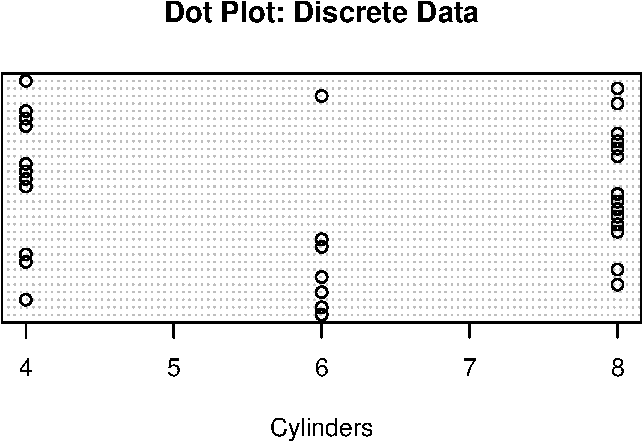
\includegraphics[keepaspectratio]{Lecture-15-Visualizations_files/figure-pdf/unnamed-chunk-1-1.pdf}}

In the visualization above we can see the number of occurrences for each
category. We can also see that 8 cylinders is the most common category
since it has the most dots. We could do something similar with
continuous data as well, but the only difference is that we will not be
able to tell which value occurs the most. We will be able to identify
where the values cluster though. For instance, in the visualization
below, I can see that the majority of the values are between 15 and 25.
Again, the y-axis does not provide any information.

\begin{Shaded}
\begin{Highlighting}[]
\FunctionTok{dotchart}\NormalTok{(mtcars}\SpecialCharTok{$}\NormalTok{mpg, }\AttributeTok{main=}\StringTok{"Dot Plot: Continuous Data"}\NormalTok{, }\AttributeTok{xlab=}\StringTok{"MPG"}\NormalTok{)}
\end{Highlighting}
\end{Shaded}

\pandocbounded{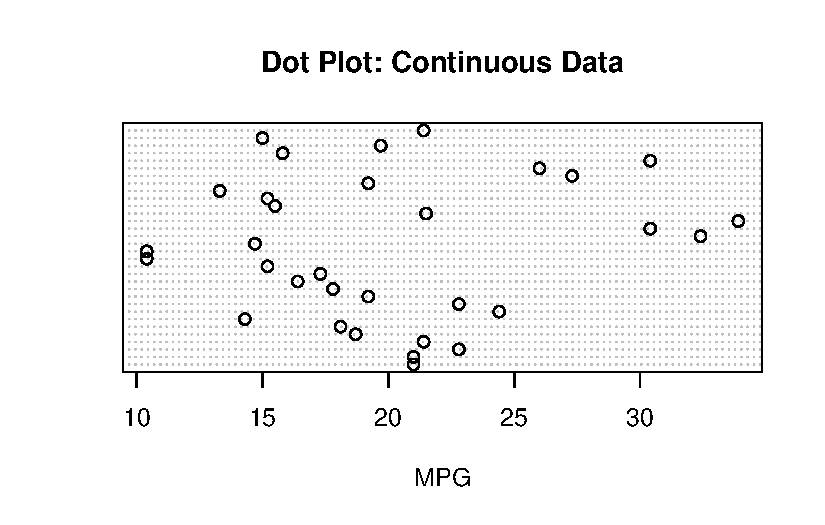
\includegraphics[keepaspectratio]{Lecture-15-Visualizations_files/figure-pdf/unnamed-chunk-2-1.pdf}}

\subsection{Histograms}\label{histograms}

We have already seen how we can visualize quantitative data with
histograms, but now we want to see the arguments we can include to
improve the visualizations. One thing we might consider doing is
altering the color of the boxes (``col'') or altering the color of the
border (``border''). We can also change the title of the plot (``main'')
and the label of the x and y-axis (``xlab'' and ``ylab''). Below is an
example of a few things we can do:

\begin{Shaded}
\begin{Highlighting}[]
 \FunctionTok{hist}\NormalTok{(mtcars}\SpecialCharTok{$}\NormalTok{mpg, }\AttributeTok{col=}\StringTok{"lightblue"}\NormalTok{, }\AttributeTok{border=}\StringTok{"red"}\NormalTok{, }
      \AttributeTok{main=}\StringTok{"Histogram of MPG"}\NormalTok{, }\AttributeTok{xlab=}\StringTok{"MPG"}\NormalTok{)}
\end{Highlighting}
\end{Shaded}

\pandocbounded{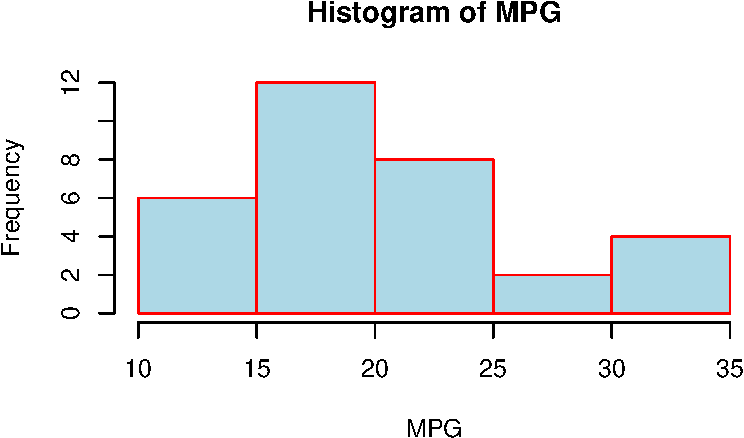
\includegraphics[keepaspectratio]{Lecture-15-Visualizations_files/figure-pdf/unnamed-chunk-3-1.pdf}}

As we have discussed before, the histograms allow us to visualize
quantitative continuous variables (or quantitative discrete if there are
a large number of possibilities) with the height of the bar representing
the number of values within the range. R will automatically choose the
number of bins and the width of the bins, but we could alter that on our
own if we wanted using the ``breaks'' argument. Passing it the number of
categories we want will be considered a suggestion and it will choose a
value near there to make the numbers work out nicely. If we pass it a
vector (just like the \emph{cut()} function) then it adhere to the cuts:

\begin{Shaded}
\begin{Highlighting}[]
\FunctionTok{hist}\NormalTok{(mtcars}\SpecialCharTok{$}\NormalTok{mpg, }\AttributeTok{breaks=}\DecValTok{10}\NormalTok{, }\AttributeTok{col=}\StringTok{"lightblue"}\NormalTok{, }
                   \AttributeTok{border=}\StringTok{"red"}\NormalTok{, }\AttributeTok{main=}\StringTok{"Histogram of MPG"}\NormalTok{, }\AttributeTok{xlab=}\StringTok{"MPG"}\NormalTok{)}
\end{Highlighting}
\end{Shaded}

\pandocbounded{\includegraphics[keepaspectratio]{Lecture-15-Visualizations_files/figure-pdf/unnamed-chunk-4-1.pdf}}

\begin{Shaded}
\begin{Highlighting}[]
\FunctionTok{hist}\NormalTok{(mtcars}\SpecialCharTok{$}\NormalTok{mpg, }\AttributeTok{breaks=}\FunctionTok{c}\NormalTok{(}\DecValTok{10}\NormalTok{,}\DecValTok{14}\NormalTok{,}\DecValTok{22}\NormalTok{,}\DecValTok{25}\NormalTok{,}\DecValTok{34}\NormalTok{), }\AttributeTok{col=}\StringTok{"lightblue"}\NormalTok{, }
                 \AttributeTok{border=}\StringTok{"red"}\NormalTok{, }\AttributeTok{main=}\StringTok{"Histogram of MPG"}\NormalTok{, }\AttributeTok{xlab=}\StringTok{"MPG"}\NormalTok{)}
\end{Highlighting}
\end{Shaded}

\pandocbounded{\includegraphics[keepaspectratio]{Lecture-15-Visualizations_files/figure-pdf/unnamed-chunk-5-1.pdf}}

\subsection{Density Plots}\label{density-plots}

Another useful plotting mechanism is the density plot. This plot will
represent the distribution of the data as a continuous function. R is
essentially telling us what distribution it thinks the data is from. We
have seen before how we can draw a density line over a histogram using
the \emph{lines()} command, but we can also just plot the density line
by itself:

\begin{Shaded}
\begin{Highlighting}[]
\FunctionTok{plot}\NormalTok{(}\FunctionTok{density}\NormalTok{(mtcars}\SpecialCharTok{$}\NormalTok{mpg))}
\end{Highlighting}
\end{Shaded}

\pandocbounded{\includegraphics[keepaspectratio]{Lecture-15-Visualizations_files/figure-pdf/unnamed-chunk-6-1.pdf}}

We could add some new elements to the visualization by changing the
limits of the x and y-axis (``xlim'' and ``ylim'') as well as using the
\emph{polygon()} function to ``fill-in'' the color below the density
line:

\begin{Shaded}
\begin{Highlighting}[]
\FunctionTok{plot}\NormalTok{(}\FunctionTok{density}\NormalTok{(mtcars}\SpecialCharTok{$}\NormalTok{mpg), }\AttributeTok{xlim=}\FunctionTok{c}\NormalTok{(}\DecValTok{5}\NormalTok{,}\DecValTok{38}\NormalTok{), }\AttributeTok{ylim=}\FunctionTok{c}\NormalTok{(}\DecValTok{0}\NormalTok{,.}\DecValTok{08}\NormalTok{), }\AttributeTok{main=}\StringTok{"Density Plot"}\NormalTok{)}
\FunctionTok{polygon}\NormalTok{(}\FunctionTok{density}\NormalTok{(mtcars}\SpecialCharTok{$}\NormalTok{mpg), }\AttributeTok{col=}\StringTok{"lightblue"}\NormalTok{, }\AttributeTok{border=}\StringTok{"red"}\NormalTok{)}
\end{Highlighting}
\end{Shaded}

\pandocbounded{\includegraphics[keepaspectratio]{Lecture-15-Visualizations_files/figure-pdf/unnamed-chunk-7-1.pdf}}

\subsection{Combining Histograms with Density
Plots}\label{combining-histograms-with-density-plots}

We have seen how we can add the density line on top of the histogram
before. Remember that when combining the histogram and the density line,
we need to specify in the histogram that frequency is false. In this
section, we will introduce a few other arguments which will assist us in
presenting the data.

\begin{Shaded}
\begin{Highlighting}[]
\FunctionTok{hist}\NormalTok{(mtcars}\SpecialCharTok{$}\NormalTok{mpg, }\AttributeTok{breaks=}\DecValTok{10}\NormalTok{, }\AttributeTok{col=}\StringTok{"lightblue"}\NormalTok{, }\AttributeTok{freq=}\ConstantTok{FALSE}\NormalTok{)}
\FunctionTok{lines}\NormalTok{(}\FunctionTok{density}\NormalTok{(mtcars}\SpecialCharTok{$}\NormalTok{mpg), }\AttributeTok{col=}\StringTok{"red"}\NormalTok{)}
\end{Highlighting}
\end{Shaded}

\pandocbounded{\includegraphics[keepaspectratio]{Lecture-15-Visualizations_files/figure-pdf/unnamed-chunk-8-1.pdf}}

We should note that whenever we start to plot something in R we will
need to create the ``canvas'' first. Essentially, we need to use a
\emph{plot(), hist(), barplot()}, or other function to make this canvas.
Then we can use \emph{lines()} to create a visualization on top of it.
So, if you were to clear the ``Plot'' pane and tried to do
``lines(density(mtcars\$mpg))'' you would get an error since there is no
canvas for it to draw this on.

We can add an additional element to the visualization called a ``rug''.
What this will do is put a line at the bottom of the graphic wherever a
data value lines on the x-axis. This will allow us to better see where
the data values are. But, if multiple values are at the same spot then
we might not be able to tell how many values are there. So, we normally
also add a ``jitter'' to it, which just adds or subtracts a small number
to it so that we can see how many values are at a single spot.

\begin{Shaded}
\begin{Highlighting}[]
\FunctionTok{hist}\NormalTok{(mtcars}\SpecialCharTok{$}\NormalTok{mpg, }\AttributeTok{breaks=}\DecValTok{10}\NormalTok{, }\AttributeTok{col=}\StringTok{"lightblue"}\NormalTok{, }\AttributeTok{freq=}\ConstantTok{FALSE}\NormalTok{)}
\FunctionTok{rug}\NormalTok{(}\FunctionTok{jitter}\NormalTok{(mtcars}\SpecialCharTok{$}\NormalTok{mpg))}
\FunctionTok{lines}\NormalTok{(}\FunctionTok{density}\NormalTok{(mtcars}\SpecialCharTok{$}\NormalTok{mpg), }\AttributeTok{col=}\StringTok{"red"}\NormalTok{)}
\end{Highlighting}
\end{Shaded}

\pandocbounded{\includegraphics[keepaspectratio]{Lecture-15-Visualizations_files/figure-pdf/unnamed-chunk-9-1.pdf}}

\subsection{Combining Histograms with Normal
Curves}\label{combining-histograms-with-normal-curves}

We can also plot the Normal Distribution over the histogram, which will
allow us to compare the data to data from a normal distribution. We will
use the same idea as the density line, except we will first need to
generate a sequence of values on the x-axis and then find the
corresponding y-value using the density of the normal distribution. As I
have said before, it is OK if we don't fully understand the code for
this part, but we should know how to use it (by altering the variables
to the variable we want to plot).

\begin{Shaded}
\begin{Highlighting}[]
\FunctionTok{hist}\NormalTok{(mtcars}\SpecialCharTok{$}\NormalTok{mpg, }\AttributeTok{breaks=}\DecValTok{10}\NormalTok{, }\AttributeTok{col=}\StringTok{"lightblue"}\NormalTok{, }\AttributeTok{freq=}\ConstantTok{FALSE}\NormalTok{)}
\NormalTok{xfit }\OtherTok{\textless{}{-}} \FunctionTok{seq}\NormalTok{(}\DecValTok{0}\NormalTok{,}\FunctionTok{max}\NormalTok{(mtcars}\SpecialCharTok{$}\NormalTok{mpg),}\AttributeTok{length=}\DecValTok{100}\NormalTok{)}
\NormalTok{yfit }\OtherTok{\textless{}{-}} \FunctionTok{dnorm}\NormalTok{(xfit,}\AttributeTok{mean=}\FunctionTok{mean}\NormalTok{(mtcars}\SpecialCharTok{$}\NormalTok{mpg),}\AttributeTok{sd=}\FunctionTok{sd}\NormalTok{(mtcars}\SpecialCharTok{$}\NormalTok{mpg))}
\FunctionTok{lines}\NormalTok{(xfit, yfit, }\AttributeTok{col=}\StringTok{"red"}\NormalTok{, }\AttributeTok{lwd=}\DecValTok{2}\NormalTok{)}
\end{Highlighting}
\end{Shaded}

\pandocbounded{\includegraphics[keepaspectratio]{Lecture-15-Visualizations_files/figure-pdf/unnamed-chunk-10-1.pdf}}

We can combine everything together and plot the histogram, the rug, the
density line, and the normal distribution all on the same plot. We can
see an example of this below, where ``lwd='' signifies the thickness of
the line and ``lty='' signifies the type of line:

\begin{Shaded}
\begin{Highlighting}[]
\FunctionTok{hist}\NormalTok{(mtcars}\SpecialCharTok{$}\NormalTok{mpg, }\AttributeTok{breaks=}\DecValTok{10}\NormalTok{, }\AttributeTok{col=}\StringTok{"lightblue"}\NormalTok{, }\AttributeTok{freq=}\ConstantTok{FALSE}\NormalTok{)}
\FunctionTok{rug}\NormalTok{(}\FunctionTok{jitter}\NormalTok{(mtcars}\SpecialCharTok{$}\NormalTok{mpg))}
\FunctionTok{lines}\NormalTok{(}\FunctionTok{density}\NormalTok{(mtcars}\SpecialCharTok{$}\NormalTok{mpg), }\AttributeTok{col=}\StringTok{"blue"}\NormalTok{, }\AttributeTok{lty=}\DecValTok{2}\NormalTok{, }\AttributeTok{lwd=}\DecValTok{2}\NormalTok{)}
\NormalTok{xfit }\OtherTok{\textless{}{-}} \FunctionTok{seq}\NormalTok{(}\DecValTok{0}\NormalTok{,}\FunctionTok{max}\NormalTok{(mtcars}\SpecialCharTok{$}\NormalTok{mpg),}\AttributeTok{length=}\DecValTok{100}\NormalTok{)}
\NormalTok{yfit }\OtherTok{\textless{}{-}} \FunctionTok{dnorm}\NormalTok{(xfit,}\AttributeTok{mean=}\FunctionTok{mean}\NormalTok{(mtcars}\SpecialCharTok{$}\NormalTok{mpg),}\AttributeTok{sd=}\FunctionTok{sd}\NormalTok{(mtcars}\SpecialCharTok{$}\NormalTok{mpg))}
\FunctionTok{lines}\NormalTok{(xfit, yfit, }\AttributeTok{col=}\StringTok{"red"}\NormalTok{, }\AttributeTok{lwd=}\DecValTok{2}\NormalTok{)}
\end{Highlighting}
\end{Shaded}

\pandocbounded{\includegraphics[keepaspectratio]{Lecture-15-Visualizations_files/figure-pdf/unnamed-chunk-11-1.pdf}}

In the plot above, we can see the density of the data with the dashed
blue line and compare it to the red line which is the normal
distribution.

\subsection{Box Plots}\label{box-plots}

Box Plots will allow us to visualize the data using the quantiles and
the IQR. This type of visualization is also called a ``Box and Whisker''
plot. The ``whiskers'' will extend out to Q1-1.5*IQR and Q3+1.5*IQR.
This will allow us to identify any outliers which may be present. The
outliers will be represented as circles if any exist. We can also use
the ``horizontal'' argument if we wish for the boxplot to be aligned
horizontally. Like all of the other visualizations, we can alter the
color and the labels using similar commands.

\begin{Shaded}
\begin{Highlighting}[]
\FunctionTok{boxplot}\NormalTok{(mtcars}\SpecialCharTok{$}\NormalTok{mpg, }\AttributeTok{col=}\StringTok{"lightblue"}\NormalTok{, }\AttributeTok{horizontal =} \ConstantTok{TRUE}\NormalTok{)}
\end{Highlighting}
\end{Shaded}

\pandocbounded{\includegraphics[keepaspectratio]{Lecture-15-Visualizations_files/figure-pdf/unnamed-chunk-12-1.pdf}}

\subsection{Quantile-Quantile Plots (QQ
Plot)}\label{quantile-quantile-plots-qq-plot}

finally, the last big visualization we want to consider is the
Quantile-Quantile Plot. This is often abbreviated as QQ Plot. This will
allow us to compare two different distribution's quantiles. We will
normally do this when we want to compare data to the normal distribution
to see if the data looks to be normal. The code below shows this
example, and what we are looking for is the data to follow the 45-degree
line. If it adheres to the line then we have even more proof of
normality.

\begin{Shaded}
\begin{Highlighting}[]
\NormalTok{data }\OtherTok{\textless{}{-}} \FunctionTok{rnorm}\NormalTok{(}\DecValTok{100}\NormalTok{,}\DecValTok{52}\NormalTok{,}\DecValTok{3}\NormalTok{)}
\FunctionTok{qqnorm}\NormalTok{(data)}
\FunctionTok{qqline}\NormalTok{(data)}
\end{Highlighting}
\end{Shaded}

\pandocbounded{\includegraphics[keepaspectratio]{Lecture-15-Visualizations_files/figure-pdf/unnamed-chunk-13-1.pdf}}

In the plot above we can see that it follows the line fairly well (which
is good since it is a normal distribution!). If it has a concave-up C
(backward C) then it would indicate a right-skewed distribution. If it
has a concave-down C (upside down C) then it would indicate a
left-skewed distribution. And finally, if it has an S pattern then the
data might be bi-modal. We will see a few of these examples below.

\subsection{Plotting Layouts}\label{plotting-layouts}

We can combine different plots using the \emph{layout()} function. This
will allow us to see multiple different plots at the same time. We will
indicate where plot 1, plot 2, etc. will go. These will then be filled
in whenever we use a plotting command.

\begin{Shaded}
\begin{Highlighting}[]
\FunctionTok{layout}\NormalTok{(}\FunctionTok{matrix}\NormalTok{(}\DecValTok{1}\SpecialCharTok{:}\DecValTok{2}\NormalTok{, }\AttributeTok{nrow=}\DecValTok{1}\NormalTok{))}
\FunctionTok{layout.show}\NormalTok{(}\DecValTok{2}\NormalTok{)}
\end{Highlighting}
\end{Shaded}

\pandocbounded{\includegraphics[keepaspectratio]{Lecture-15-Visualizations_files/figure-pdf/unnamed-chunk-14-1.pdf}}

Now we will see how we can use 2 different plots at the same time. We
should also notice how the QQ plot looks when our data is symmetrical or
skewed.

\begin{Shaded}
\begin{Highlighting}[]
\FunctionTok{library}\NormalTok{(openintro)}
\end{Highlighting}
\end{Shaded}

\begin{Shaded}
\begin{Highlighting}[]
\FunctionTok{hist}\NormalTok{(babies}\SpecialCharTok{$}\NormalTok{bwt, }\AttributeTok{col=}\StringTok{"lightblue"}\NormalTok{, }\AttributeTok{main=}\StringTok{"Symmetric Data"}\NormalTok{)}
\FunctionTok{qqnorm}\NormalTok{(babies}\SpecialCharTok{$}\NormalTok{bwt)}
\FunctionTok{qqline}\NormalTok{(babies}\SpecialCharTok{$}\NormalTok{bwt, }\AttributeTok{col=}\StringTok{"red"}\NormalTok{, }\AttributeTok{lwd=}\DecValTok{2}\NormalTok{)}
\end{Highlighting}
\end{Shaded}

\pandocbounded{\includegraphics[keepaspectratio]{Lecture-15-Visualizations_files/figure-pdf/unnamed-chunk-17-1.pdf}}

\begin{Shaded}
\begin{Highlighting}[]
\FunctionTok{hist}\NormalTok{(mlb\_teams}\SpecialCharTok{$}\NormalTok{triples, }\AttributeTok{main=}\StringTok{"Right Skewed"}\NormalTok{, }\AttributeTok{col=}\StringTok{"lightblue"}\NormalTok{)}
\FunctionTok{qqnorm}\NormalTok{(mlb\_teams}\SpecialCharTok{$}\NormalTok{triples)}
\FunctionTok{qqline}\NormalTok{(mlb\_teams}\SpecialCharTok{$}\NormalTok{triples, }\AttributeTok{col=}\StringTok{"red"}\NormalTok{, }\AttributeTok{lwd=}\DecValTok{2}\NormalTok{)}
\end{Highlighting}
\end{Shaded}

\pandocbounded{\includegraphics[keepaspectratio]{Lecture-15-Visualizations_files/figure-pdf/unnamed-chunk-19-1.pdf}}

\begin{Shaded}
\begin{Highlighting}[]
\FunctionTok{hist}\NormalTok{(mlb\_teams}\SpecialCharTok{$}\NormalTok{hits, }\AttributeTok{main=}\StringTok{"Left Skewed"}\NormalTok{, }\AttributeTok{col=}\StringTok{"lightblue"}\NormalTok{)}
\FunctionTok{qqnorm}\NormalTok{(mlb\_teams}\SpecialCharTok{$}\NormalTok{hits)}
\FunctionTok{qqline}\NormalTok{(mlb\_teams}\SpecialCharTok{$}\NormalTok{hits, }\AttributeTok{col=}\StringTok{"red"}\NormalTok{, }\AttributeTok{lwd=}\DecValTok{2}\NormalTok{)}
\end{Highlighting}
\end{Shaded}

\pandocbounded{\includegraphics[keepaspectratio]{Lecture-15-Visualizations_files/figure-pdf/unnamed-chunk-21-1.pdf}}

\begin{Shaded}
\begin{Highlighting}[]
\FunctionTok{hist}\NormalTok{(mlb\_teams}\SpecialCharTok{$}\NormalTok{homeruns, }\AttributeTok{main=}\StringTok{"Left Skewed"}\NormalTok{, }\AttributeTok{col=}\StringTok{"lightblue"}\NormalTok{)}
\FunctionTok{qqnorm}\NormalTok{(mlb\_teams}\SpecialCharTok{$}\NormalTok{homeruns)}
\FunctionTok{qqline}\NormalTok{(mlb\_teams}\SpecialCharTok{$}\NormalTok{homeruns, }\AttributeTok{col=}\StringTok{"red"}\NormalTok{, }\AttributeTok{lwd=}\DecValTok{2}\NormalTok{)}
\end{Highlighting}
\end{Shaded}

\pandocbounded{\includegraphics[keepaspectratio]{Lecture-15-Visualizations_files/figure-pdf/unnamed-chunk-23-1.pdf}}

We can alter the plot even more if we want to include another type of
plot as well. We could have as many as we would want really, but it is
typical to only plot between 1 and 4 things in a single window. The
example below plots it as a single thing on the top and 2 things on the
bottom:

\begin{Shaded}
\begin{Highlighting}[]
\FunctionTok{layout}\NormalTok{(}\FunctionTok{matrix}\NormalTok{(}\FunctionTok{c}\NormalTok{(}\DecValTok{1}\NormalTok{,}\DecValTok{1}\NormalTok{,}\DecValTok{2}\NormalTok{,}\DecValTok{3}\NormalTok{),}\DecValTok{2}\NormalTok{,}\DecValTok{2}\NormalTok{,}\AttributeTok{byrow=}\ConstantTok{TRUE}\NormalTok{))}
\FunctionTok{hist}\NormalTok{(mtcars}\SpecialCharTok{$}\NormalTok{mpg, }\AttributeTok{breaks=}\DecValTok{10}\NormalTok{, }\AttributeTok{col=}\StringTok{"lightblue"}\NormalTok{, }\AttributeTok{main=}\StringTok{"Historgram of MPG"}\NormalTok{, }
     \AttributeTok{xlab=}\StringTok{"MPG"}\NormalTok{, }\AttributeTok{freq=}\ConstantTok{FALSE}\NormalTok{)}
\FunctionTok{rug}\NormalTok{(}\FunctionTok{jitter}\NormalTok{(mtcars}\SpecialCharTok{$}\NormalTok{mpg))}
\FunctionTok{lines}\NormalTok{(}\FunctionTok{density}\NormalTok{(mtcars}\SpecialCharTok{$}\NormalTok{mpg), }\AttributeTok{col=}\StringTok{"blue"}\NormalTok{, }\AttributeTok{lty=}\DecValTok{2}\NormalTok{, }\AttributeTok{lwd=}\DecValTok{2}\NormalTok{)}
\NormalTok{xfit }\OtherTok{\textless{}{-}} \FunctionTok{seq}\NormalTok{(}\DecValTok{0}\NormalTok{,}\FunctionTok{max}\NormalTok{(mtcars}\SpecialCharTok{$}\NormalTok{mpg),}\AttributeTok{length=}\DecValTok{100}\NormalTok{)}
\NormalTok{yfit }\OtherTok{\textless{}{-}} \FunctionTok{dnorm}\NormalTok{(xfit,}\AttributeTok{mean=}\FunctionTok{mean}\NormalTok{(mtcars}\SpecialCharTok{$}\NormalTok{mpg),}\AttributeTok{sd=}\FunctionTok{sd}\NormalTok{(mtcars}\SpecialCharTok{$}\NormalTok{mpg))}
\FunctionTok{lines}\NormalTok{(xfit, yfit, }\AttributeTok{col=}\StringTok{"red"}\NormalTok{, }\AttributeTok{lwd=}\DecValTok{2}\NormalTok{)}
\FunctionTok{boxplot}\NormalTok{(mtcars}\SpecialCharTok{$}\NormalTok{mpg, }\AttributeTok{col=}\StringTok{"lightblue"}\NormalTok{, }\AttributeTok{horizontal =} \ConstantTok{TRUE}\NormalTok{)}
\FunctionTok{qqnorm}\NormalTok{(mtcars}\SpecialCharTok{$}\NormalTok{mpg)}
\FunctionTok{qqline}\NormalTok{(mtcars}\SpecialCharTok{$}\NormalTok{mpg, }\AttributeTok{col=}\StringTok{"red"}\NormalTok{, }\AttributeTok{lwd=}\DecValTok{2}\NormalTok{)}
\end{Highlighting}
\end{Shaded}

\pandocbounded{\includegraphics[keepaspectratio]{Lecture-15-Visualizations_files/figure-pdf/unnamed-chunk-24-1.pdf}}

We can get back to the original plotting window by using the following
command:

\begin{Shaded}
\begin{Highlighting}[]
\FunctionTok{par}\NormalTok{(}\AttributeTok{mfrow=}\FunctionTok{c}\NormalTok{(}\DecValTok{1}\NormalTok{,}\DecValTok{1}\NormalTok{))}
\end{Highlighting}
\end{Shaded}

\section{Qualitative Visualizations}\label{qualitative-visualizations}

We have seen several ways we can visualize quantitative data with dot
plots, histograms, density plots, and box plots. However, we have to use
a different approach if we wish to visualize qualitative data since
these are categories and not necessarily numbers. One of the easiest
(and potentially the best) ways to describe categorical data is to
either use counts or proportions. Since it does not necessarily make
sense to find the mean of categorical data, we just want to count the
number of observations in the category

\subsection{Frequency Tables}\label{frequency-tables}

We can calculate the number of values in each category relatively easily
using the \emph{table()} function. We have already seen this command
before, and have used it to summarize categories (and quantitative
discrete when there are relatively few possible outcomes). Below is an
example of this function using the `mlb\_players\_18' dataset from the
`openintro' library:

\begin{Shaded}
\begin{Highlighting}[]
\FunctionTok{table}\NormalTok{(mlb\_players\_18}\SpecialCharTok{$}\NormalTok{position)}
\end{Highlighting}
\end{Shaded}

\begin{verbatim}

 1B  2B  3B   C  CF  DH  LF   P  RF  SS 
 59  83  73 115  79   6  70 642  76  67 
\end{verbatim}

We can place the table function within the \emph{addmargins()} function
to print out the total of all of the counts.

\begin{Shaded}
\begin{Highlighting}[]
\FunctionTok{addmargins}\NormalTok{(}\FunctionTok{table}\NormalTok{(mlb\_players\_18}\SpecialCharTok{$}\NormalTok{position))}
\end{Highlighting}
\end{Shaded}

\begin{verbatim}

  1B   2B   3B    C   CF   DH   LF    P   RF   SS  Sum 
  59   83   73  115   79    6   70  642   76   67 1270 
\end{verbatim}

If instead of counts we wanted to calculate the proportion of values in
each category, we can do that by dividing the table by the number of
observations we have. This can easily be done since everything in R is a
vector. I have included the \emph{round()} function and selected 3
decimal places since we do not need to be too precise:

\begin{Shaded}
\begin{Highlighting}[]
\FunctionTok{round}\NormalTok{(}\FunctionTok{table}\NormalTok{(mlb\_players\_18}\SpecialCharTok{$}\NormalTok{position)}\SpecialCharTok{/}\FunctionTok{length}\NormalTok{(mlb\_players\_18}\SpecialCharTok{$}\NormalTok{position),}\DecValTok{3}\NormalTok{)}
\end{Highlighting}
\end{Shaded}

\begin{verbatim}

   1B    2B    3B     C    CF    DH    LF     P    RF    SS 
0.046 0.065 0.057 0.091 0.062 0.005 0.055 0.506 0.060 0.053 
\end{verbatim}

Likewise, if we wanted the percentage of values in each category we
could multiply the expression above by 100 and it will convert the
values from proportions to percentages. Another way we could carry out
this same task would be to use the \emph{prop.table()} function. It may
be hard to memorize all of these functions, but just remember that there
are multiple ways to do things in R, so we can use whatever we are most
comfortable with:

\begin{Shaded}
\begin{Highlighting}[]
\FunctionTok{round}\NormalTok{(}\FunctionTok{prop.table}\NormalTok{(}\FunctionTok{table}\NormalTok{(mlb\_players\_18}\SpecialCharTok{$}\NormalTok{position)),}\DecValTok{3}\NormalTok{)}
\end{Highlighting}
\end{Shaded}

\begin{verbatim}

   1B    2B    3B     C    CF    DH    LF     P    RF    SS 
0.046 0.065 0.057 0.091 0.062 0.005 0.055 0.506 0.060 0.053 
\end{verbatim}

\begin{Shaded}
\begin{Highlighting}[]
\FunctionTok{addmargins}\NormalTok{(}\FunctionTok{round}\NormalTok{(}\FunctionTok{prop.table}\NormalTok{(}\FunctionTok{table}\NormalTok{(mlb\_players\_18}\SpecialCharTok{$}\NormalTok{position)),}\DecValTok{3}\NormalTok{))}
\end{Highlighting}
\end{Shaded}

\begin{verbatim}

   1B    2B    3B     C    CF    DH    LF     P    RF    SS   Sum 
0.046 0.065 0.057 0.091 0.062 0.005 0.055 0.506 0.060 0.053 1.000 
\end{verbatim}

\begin{Shaded}
\begin{Highlighting}[]
\FunctionTok{addmargins}\NormalTok{(}\FunctionTok{round}\NormalTok{(}\FunctionTok{prop.table}\NormalTok{(}\FunctionTok{table}\NormalTok{(mlb\_players\_18}\SpecialCharTok{$}\NormalTok{position)),}\DecValTok{3}\NormalTok{))}\SpecialCharTok{*}\DecValTok{100}
\end{Highlighting}
\end{Shaded}

\begin{verbatim}

   1B    2B    3B     C    CF    DH    LF     P    RF    SS   Sum 
  4.6   6.5   5.7   9.1   6.2   0.5   5.5  50.6   6.0   5.3 100.0 
\end{verbatim}

\subsection{Pie Chart}\label{pie-chart}

One common way to visualize categorical data is through the use of a pie
chart. This type of visualization allows us to compare the percentages
across categories. While this is the most popular method, it is often
hard to compare categories, especially when there are a large number of
levels. Doing a pie chart in R is a little challenging, as the user must
pass the function the percentage of each category and not just the
table. Additionally, to get meaningful labels, the user must create
those as well:

\begin{Shaded}
\begin{Highlighting}[]
\NormalTok{table\_cat }\OtherTok{\textless{}{-}} \FunctionTok{table}\NormalTok{(mlb\_players\_18}\SpecialCharTok{$}\NormalTok{position)}
\NormalTok{percent\_cat }\OtherTok{\textless{}{-}} \FunctionTok{round}\NormalTok{(}\FunctionTok{prop.table}\NormalTok{(table\_cat),}\DecValTok{3}\NormalTok{)}\SpecialCharTok{*}\DecValTok{100}
\NormalTok{my\_labels }\OtherTok{\textless{}{-}} \FunctionTok{paste0}\NormalTok{(}\FunctionTok{names}\NormalTok{(percent\_cat), }\StringTok{": "}\NormalTok{, percent\_cat, }\StringTok{"\%"}\NormalTok{)}
\FunctionTok{pie}\NormalTok{(table\_cat, }\AttributeTok{labels=}\NormalTok{my\_labels, }\AttributeTok{main=}\StringTok{"Pie Chart of Positions Played"}\NormalTok{, }
    \AttributeTok{col=}\FunctionTok{rainbow}\NormalTok{(}\FunctionTok{length}\NormalTok{(table\_cat)))}
\end{Highlighting}
\end{Shaded}

\pandocbounded{\includegraphics[keepaspectratio]{Lecture-15-Visualizations_files/figure-pdf/unnamed-chunk-30-1.pdf}}

As we can see from the visualization above, it is hard to read a pie
chart when there are a lot of different categories. We could try to
simplify it though by making a new column and combining a few
categories:

\begin{Shaded}
\begin{Highlighting}[]
\NormalTok{mlb\_players\_18 }\OtherTok{\textless{}{-}} \FunctionTok{data.frame}\NormalTok{(mlb\_players\_18)}
\NormalTok{mlb\_players\_18}\SpecialCharTok{$}\NormalTok{position\_cat }\OtherTok{\textless{}{-}} \ConstantTok{NA}

\NormalTok{mlb\_players\_18[mlb\_players\_18}\SpecialCharTok{$}\NormalTok{position }\SpecialCharTok{\%in\%} 
                 \FunctionTok{c}\NormalTok{(}\StringTok{"1B"}\NormalTok{, }\StringTok{"2B"}\NormalTok{, }\StringTok{"3B"}\NormalTok{, }\StringTok{"SS"}\NormalTok{) ,]}\SpecialCharTok{$}\NormalTok{position\_cat }\OtherTok{\textless{}{-}} \StringTok{"Infield"}

\NormalTok{mlb\_players\_18[mlb\_players\_18}\SpecialCharTok{$}\NormalTok{position }\SpecialCharTok{\%in\%} 
                 \FunctionTok{c}\NormalTok{(}\StringTok{"LF"}\NormalTok{, }\StringTok{"CF"}\NormalTok{, }\StringTok{"RF"}\NormalTok{) ,]}\SpecialCharTok{$}\NormalTok{position\_cat }\OtherTok{\textless{}{-}} \StringTok{"Outfield"}

\NormalTok{mlb\_players\_18[mlb\_players\_18}\SpecialCharTok{$}\NormalTok{position}\SpecialCharTok{==}\StringTok{"P"}\NormalTok{,]}\SpecialCharTok{$}\NormalTok{position\_cat }\OtherTok{\textless{}{-}} \StringTok{"Pitcher"}

\NormalTok{mlb\_players\_18[mlb\_players\_18}\SpecialCharTok{$}\NormalTok{position }\SpecialCharTok{\%in\%} 
                 \FunctionTok{c}\NormalTok{(}\StringTok{"C"}\NormalTok{, }\StringTok{"DH"}\NormalTok{),]}\SpecialCharTok{$}\NormalTok{position\_cat }\OtherTok{\textless{}{-}} \StringTok{"Other"}

\NormalTok{table\_cat }\OtherTok{\textless{}{-}} \FunctionTok{table}\NormalTok{(mlb\_players\_18}\SpecialCharTok{$}\NormalTok{position\_cat)}
\NormalTok{table\_cat}
\end{Highlighting}
\end{Shaded}

\begin{verbatim}

 Infield    Other Outfield  Pitcher 
     282      121      225      642 
\end{verbatim}

\begin{Shaded}
\begin{Highlighting}[]
\NormalTok{percent\_cat }\OtherTok{\textless{}{-}} \FunctionTok{round}\NormalTok{(}\FunctionTok{prop.table}\NormalTok{(table\_cat),}\DecValTok{3}\NormalTok{)}\SpecialCharTok{*}\DecValTok{100}
\NormalTok{my\_labels }\OtherTok{\textless{}{-}} \FunctionTok{paste0}\NormalTok{(}\FunctionTok{names}\NormalTok{(percent\_cat), }\StringTok{": "}\NormalTok{, percent\_cat, }\StringTok{"\%"}\NormalTok{)}
\FunctionTok{pie}\NormalTok{(table\_cat, }\AttributeTok{labels=}\NormalTok{my\_labels, }\AttributeTok{main=}\StringTok{"Pie Chart of Positions Played"}\NormalTok{, }
    \AttributeTok{col=}\FunctionTok{rainbow}\NormalTok{(}\FunctionTok{length}\NormalTok{(table\_cat)))}
\end{Highlighting}
\end{Shaded}

\pandocbounded{\includegraphics[keepaspectratio]{Lecture-15-Visualizations_files/figure-pdf/unnamed-chunk-31-1.pdf}}

\subsection{Fan Plots}\label{fan-plots}

Another way we can visualize categorical data is to use a Fan Plot. This
method is comparable to the pie chart as the size of the sections
relates to the percentage of values in the category. The main difference
though is that it overlays the visualizations, allowing one to easily
compare the sizes of the different categories. The function relies on
the `plotrix' package, which may need to be installed before using it if
is the first time using it.

\begin{Shaded}
\begin{Highlighting}[]
\FunctionTok{library}\NormalTok{(plotrix)}
\NormalTok{table\_cat }\OtherTok{\textless{}{-}} \FunctionTok{table}\NormalTok{(mlb\_players\_18}\SpecialCharTok{$}\NormalTok{position\_cat)}
\NormalTok{percent\_cat }\OtherTok{\textless{}{-}} \FunctionTok{round}\NormalTok{(}\FunctionTok{prop.table}\NormalTok{(table\_cat),}\DecValTok{3}\NormalTok{)}\SpecialCharTok{*}\DecValTok{100}
\NormalTok{my\_labels }\OtherTok{\textless{}{-}} \FunctionTok{paste0}\NormalTok{(}\FunctionTok{names}\NormalTok{(percent\_cat), }\StringTok{": "}\NormalTok{, percent\_cat, }\StringTok{"\%"}\NormalTok{)}
\FunctionTok{fan.plot}\NormalTok{(table\_cat, }\AttributeTok{labels=}\NormalTok{my\_labels, }
         \AttributeTok{main=}\StringTok{"Fan Plot of Positions Played"}\NormalTok{, }\AttributeTok{col=}\FunctionTok{rainbow}\NormalTok{(}\FunctionTok{length}\NormalTok{(table\_cat)))}
\end{Highlighting}
\end{Shaded}

\pandocbounded{\includegraphics[keepaspectratio]{Lecture-15-Visualizations_files/figure-pdf/unnamed-chunk-32-1.pdf}}

\subsection{Bar Plots}\label{bar-plots}

While histograms are used for quantitative data, bar plots can be used
for qualitative data. We have seen this process before, as we have to
pass a table into the \emph{barplot()} function.

\begin{Shaded}
\begin{Highlighting}[]
\FunctionTok{barplot}\NormalTok{(}\FunctionTok{table}\NormalTok{(mlb\_players\_18}\SpecialCharTok{$}\NormalTok{position\_cat), }
        \AttributeTok{col=}\FunctionTok{c}\NormalTok{(}\StringTok{"red"}\NormalTok{, }\StringTok{"blue"}\NormalTok{, }\StringTok{"green"}\NormalTok{, }\StringTok{"purple"}\NormalTok{), }
        \AttributeTok{main=}\StringTok{"Barplot of Positions"}\NormalTok{, }\AttributeTok{xlab=}\StringTok{"Positions"}\NormalTok{)}
\end{Highlighting}
\end{Shaded}

\pandocbounded{\includegraphics[keepaspectratio]{Lecture-15-Visualizations_files/figure-pdf/unnamed-chunk-33-1.pdf}}

If there are a large number of categories, the visualization might not
print out all of the category names. On the plot below, notice how all
of the category's names are not printed out under the columns due to
spacing issues:

\begin{Shaded}
\begin{Highlighting}[]
\FunctionTok{barplot}\NormalTok{(}\FunctionTok{table}\NormalTok{(mlb\_players\_18}\SpecialCharTok{$}\NormalTok{position), }
        \AttributeTok{col=}\FunctionTok{rainbow}\NormalTok{(}\DecValTok{10}\NormalTok{), }\AttributeTok{main=}\StringTok{"Barplot of Positions"}\NormalTok{)}
\end{Highlighting}
\end{Shaded}

\pandocbounded{\includegraphics[keepaspectratio]{Lecture-15-Visualizations_files/figure-pdf/unnamed-chunk-34-1.pdf}}

If this happens, we could try making the plot region bigger or
condensing our categories (if it makes sense to do so). Another solution
would be to include the `las=2' argument, which formats the labels to be
perpendicular to the x-axis. This will allow us to see each category
name a little easier.

\begin{Shaded}
\begin{Highlighting}[]
\FunctionTok{barplot}\NormalTok{(}\FunctionTok{table}\NormalTok{(mlb\_players\_18}\SpecialCharTok{$}\NormalTok{position), }\AttributeTok{col=}\FunctionTok{rainbow}\NormalTok{(}\DecValTok{10}\NormalTok{), }
        \AttributeTok{las=}\DecValTok{2}\NormalTok{, }\AttributeTok{main=}\StringTok{"Barplot of Positions"}\NormalTok{)}
\end{Highlighting}
\end{Shaded}

\pandocbounded{\includegraphics[keepaspectratio]{Lecture-15-Visualizations_files/figure-pdf/unnamed-chunk-35-1.pdf}}

\subsection{Waffle Plot}\label{waffle-plot}

The Waffle Plot is similar to the pie chart but it creates little
squares for each category. The more squares a category has the more
observations there are. This easily allows one to compare different
groups. It should be mentioned that the squares are scaled by a vector
of values (we can decide how much each square is ``worth''). For this
graphic, we will need the `waffle' package, which may need to be
installed before using it if is the first time using it.

\begin{Shaded}
\begin{Highlighting}[]
\FunctionTok{library}\NormalTok{(waffle)}
\NormalTok{bcnt }\OtherTok{\textless{}{-}} \FunctionTok{as.vector}\NormalTok{(}\FunctionTok{table}\NormalTok{(mlb\_players\_18}\SpecialCharTok{$}\NormalTok{position))}
\FunctionTok{names}\NormalTok{(bcnt) }\OtherTok{\textless{}{-}} \FunctionTok{names}\NormalTok{(}\FunctionTok{table}\NormalTok{(mlb\_players\_18}\SpecialCharTok{$}\NormalTok{position))}
\FunctionTok{waffle}\NormalTok{(bcnt}\SpecialCharTok{/}\DecValTok{10}\NormalTok{, }\AttributeTok{rows=}\DecValTok{8}\NormalTok{, }\AttributeTok{col=}\FunctionTok{rainbow}\NormalTok{(}\DecValTok{10}\NormalTok{), }
       \AttributeTok{title=}\StringTok{"Waffle Plot of Position Players"}\NormalTok{, }
       \AttributeTok{xlab=}\StringTok{"1 square=10 players"}\NormalTok{)}
\end{Highlighting}
\end{Shaded}

\pandocbounded{\includegraphics[keepaspectratio]{Lecture-15-Visualizations_files/figure-pdf/unnamed-chunk-36-1.pdf}}

\subsection{Pareto Chart}\label{pareto-chart}

The last visualization type we will discuss in this section is the
Pareto Chart. This is a chart that is very similar to the bar chart,
except the categories are sorted in order from largest to smallest. This
allows for the comparison of similarly sized groups. An additional
element typically included is the cumulative percentage of occurrences.
This will allow you to see what percentage of the observations are in
the category or the categories that have come before it. This graphic
relies on the `qcc' package, which may need to be installed before using
it if is the first time using it.

\begin{Shaded}
\begin{Highlighting}[]
\FunctionTok{library}\NormalTok{(qcc)}
\NormalTok{bcnt }\OtherTok{\textless{}{-}} \FunctionTok{as.vector}\NormalTok{(}\FunctionTok{table}\NormalTok{(mlb\_players\_18}\SpecialCharTok{$}\NormalTok{position))}
\FunctionTok{names}\NormalTok{(bcnt) }\OtherTok{\textless{}{-}} \FunctionTok{names}\NormalTok{(}\FunctionTok{table}\NormalTok{(mlb\_players\_18}\SpecialCharTok{$}\NormalTok{position))}
\NormalTok{y }\OtherTok{\textless{}{-}} \FunctionTok{pareto.chart}\NormalTok{(bcnt,}\AttributeTok{main=}\StringTok{"Pareto Chart Positions"}\NormalTok{,}
                  \AttributeTok{xlab=}\StringTok{"Alignment"}\NormalTok{)}
\end{Highlighting}
\end{Shaded}

\pandocbounded{\includegraphics[keepaspectratio]{Lecture-15-Visualizations_files/figure-pdf/unnamed-chunk-37-1.pdf}}

We can see this with fewer categories as well and can see the amount in
each category plus the percentage of observations in the category and
the categories before it.

\begin{Shaded}
\begin{Highlighting}[]
\NormalTok{bcnt }\OtherTok{\textless{}{-}} \FunctionTok{as.vector}\NormalTok{(}\FunctionTok{table}\NormalTok{(mlb\_players\_18}\SpecialCharTok{$}\NormalTok{position\_cat))}
\FunctionTok{names}\NormalTok{(bcnt) }\OtherTok{\textless{}{-}} \FunctionTok{names}\NormalTok{(}\FunctionTok{table}\NormalTok{(mlb\_players\_18}\SpecialCharTok{$}\NormalTok{position\_cat))}
\FunctionTok{pareto.chart}\NormalTok{(bcnt,}\AttributeTok{main=}\StringTok{"Pareto Chart Positions"}\NormalTok{,}
             \AttributeTok{xlab=}\StringTok{"Alignment"}\NormalTok{)}
\end{Highlighting}
\end{Shaded}

\pandocbounded{\includegraphics[keepaspectratio]{Lecture-15-Visualizations_files/figure-pdf/unnamed-chunk-38-1.pdf}}

\begin{verbatim}
          
Pareto chart analysis for bcnt
             Frequency   Cum.Freq.  Percentage Cum.Percent.
  Pitcher   642.000000  642.000000   50.551181    50.551181
  Infield   282.000000  924.000000   22.204724    72.755906
  Outfield  225.000000 1149.000000   17.716535    90.472441
  Other     121.000000 1270.000000    9.527559   100.000000
\end{verbatim}




\end{document}
